%%%%%%%%%%%%%%%%%%%%%%%%%%%%%%%%%%%%%%%%%%%%%%%%%%%%%%%%%%%%%%%
%% OXFORD THESIS TEMPLATE

% Use this template to produce a standard thesis that meets the Oxford University requirements for DPhil submission
%
% Originally by Keith A. Gillow (gillow@maths.ox.ac.uk), 1997
% Modified by Sam Evans (sam@samuelevansresearch.org), 2007
% Modified by John McManigle (john@oxfordechoes.com), 2015
%
% This version Copyright (c) 2015-2023 John McManigle
%
% Broad permissions are granted to use, modify, and distribute this software
% as specified in the MIT License included in this distribution's LICENSE file.
%

% I've (John) tried to comment this file extensively, so read through it to see how to use the various options.  Remember
% that in LaTeX, any line starting with a % is NOT executed.  Several places below, you have a choice of which line to use
% out of multiple options (eg draft vs final, for PDF vs for binding, etc.)  When you pick one, add a % to the beginning of
% the lines you don't want.


%%%%% CHOOSE PAGE LAYOUT
% The most common choices should be below.  You can also do other things, like replacing "a4paper" with "letterpaper", etc.

% This one will format for two-sided binding (ie left and right pages have mirror margins; blank pages inserted where needed):
%\documentclass[a4paper,twoside]{ociamthesis}
% This one will format for one-sided binding (ie left margin > right margin; no extra blank pages):
%\documentclass[a4paper]{ociamthesis}
% This one will format for PDF output (ie equal margins, no extra blank pages):
\documentclass[a4paper,nobind]{ociamthesis} 



%%%%% SELECT YOUR DRAFT OPTIONS
% Three options going on here; use in any combination.  But remember to turn the first two off before
% generating a PDF to send to the printer!

% This adds a "DRAFT" footer to every normal page.  (The first page of each chapter is not a "normal" page.)
%\fancyfoot[C]{\emph{DRAFT Printed on \today}}  

% This highlights (in blue) corrections marked with (for words) \mccorrect{blah} or (for whole
% paragraphs) \begin{mccorrection} . . . \end{mccorrection}.  This can be useful for sending a PDF of
% your corrected thesis to your examiners for review.  Turn it off, and the blue disappears.
%\correctionstrue


%%%%% BIBLIOGRAPHY SETUP
% Note that your bibliography will require some tweaking depending on your department, preferred format, etc.
% The options included below are just very basic "sciencey" and "humanitiesey" options to get started.
% If you've not used LaTeX before, I recommend reading a little about biblatex/biber and getting started with it.
% If you're already a LaTeX pro and are used to natbib or something, modify as necessary.
% Either way, you'll have to choose and configure an appropriate bibliography format...

% The science-type option: numerical in-text citation with references in order of appearance.
\usepackage[style=numeric-comp, sorting=none, backend=biber, doi=false, isbn=false]{biblatex}
\newcommand*{\bibtitle}{References}

% The humanities-type option: author-year in-text citation with an alphabetical works cited.
%\usepackage[style=authoryear, sorting=nyt, backend=biber, maxcitenames=2, useprefix, doi=false, isbn=false]{biblatex}
%\newcommand*{\bibtitle}{Works Cited}

% This makes the bibliography left-aligned (not 'justified') and slightly smaller font.
\renewcommand*{\bibfont}{\raggedright\small}

% Change this to the name of your .bib file (usually exported from a citation manager like Zotero or EndNote).
\addbibresource{references.bib}


% Uncomment this if you want equation numbers per section (2.3.12), instead of per chapter (2.18):
%\numberwithin{equation}{subsection}



%%%%% THESIS / TITLE PAGE INFORMATION
% Everybody needs to complete the following:
\title{Next-Generation Neutrino Interaction Measurements and Beyond-Standard-Model Physics with the Upgraded T2K Near Detector}
\author{Weijun Li}
\college{The Queen's College}

% Master's candidates who require the alternate title page (with candidate number and word count)
% must also un-comment and complete the following three lines:
%\masterssubmissiontrue
%\candidateno{933516}
%\wordcount{28,815}

% Uncomment the following line if your degree also includes exams (eg most masters):
%\renewcommand{\submittedtext}{Submitted in partial completion of the}
% Your full degree name.  (But remember that DPhils aren't "in" anything.  They're just DPhils.)
\degree{Doctor of Philosophy}
% Term and year of submission, or date if your board requires (eg most masters)
\degreedate{Hilary 2025}


%%%%% YOUR OWN PERSONAL MACROS
% This is a good place to dump your own LaTeX macros as they come up.

% To make text superscripts shortcuts
	\renewcommand{\th}{\textsuperscript{th}} % ex: I won 4\th place
	\newcommand{\nd}{\textsuperscript{nd}}
	\renewcommand{\st}{\textsuperscript{st}}
	\newcommand{\rd}{\textsuperscript{rd}}

%%%%% THE ACTUAL DOCUMENT STARTS HERE
\begin{document}



%%%%% CHOOSE YOUR LINE SPACING HERE
% This is the official option.  Use it for your submission copy and library copy:
\setlength{\textbaselineskip}{22pt plus2pt}
% This is closer spacing (about 1.5-spaced) that you might prefer for your personal copies:
%\setlength{\textbaselineskip}{18pt plus2pt minus1pt}

% You can set the spacing here for the roman-numbered pages (acknowledgements, table of contents, etc.)
\setlength{\frontmatterbaselineskip}{17pt plus1pt minus1pt}

% Leave this line alone; it gets things started for the real document.
\setlength{\baselineskip}{\textbaselineskip}


%%%%% CHOOSE YOUR SECTION NUMBERING DEPTH HERE
% You have two choices.  First, how far down are sections numbered?  (Below that, they're named but
% don't get numbers.)  Second, what level of section appears in the table of contents?  These don't have
% to match: you can have numbered sections that don't show up in the ToC, or unnumbered sections that
% do.  Throughout, 0 = chapter; 1 = section; 2 = subsection; 3 = subsubsection, 4 = paragraph...

% The level that gets a number:
\setcounter{secnumdepth}{2}
% The level that shows up in the ToC:
\setcounter{tocdepth}{2}


%%%%% ABSTRACT SEPARATE
% This is used to create the separate, one-page abstract that you are required to hand into the Exam
% Schools.  You can comment it out to generate a PDF for printing or whatnot.
\begin{abstractseparate}
	Your abstract text goes here.  Check your departmental regulations, but generally this should be less than 300 words.  See the beginning of Chapter~\ref{ch:2-litreview} for more.

Worked on upgrade, new physics potential

Did a few analyses based on the upgrade:
    - ESC
    - TL pi
    - COM
    - TKI

However, not enough time to look at data, hence did a tuning project and a sens extraction. % Create an abstract.tex file in the 'text' folder for your abstract.
\end{abstractseparate}


% JEM: Pages are roman numbered from here, though page numbers are invisible until ToC.  This is in
% keeping with most typesetting conventions.
\begin{romanpages}

% JEM: By default, this template uses the traditional Oxford "Belt Crest". Un-comment the following
% line to use the newer, "Blue Square" logo:
% \renewcommand{\crest}{{\includegraphics[width=4.2cm, height=4.2cm]{figures/newlogo.pdf}}}

% Title page is created here
\maketitle

%%%%% DEDICATION -- If you'd like one, un-comment the following.
%\begin{dedication}
%This thesis is dedicated to\\
%someone\\
%for some special reason\\
%\end{dedication}

%%%%% ACKNOWLEDGEMENTS -- Nothing to do here except comment out if you don't want it.
\begin{acknowledgements}
 	\subsection*{Personal}

Thank you!!!!!

% \subsection*{Institutional}

% If you want to separate out your thanks for funding and institutional support, I don't think there's any rule against it.  Of course, you could also just remove the subsections and do one big traditional acknowledgement section.

% Lorem ipsum dolor sit amet, consectetur adipiscing elit. Ut luctus tempor ex at pretium. Sed varius, mauris at dapibus lobortis, elit purus tempor neque, facilisis sollicitudin felis nunc a urna. Morbi mattis ante non augue blandit pulvinar. Quisque nec euismod mauris. Nulla et tellus eu nibh auctor malesuada quis imperdiet quam. Sed eget tincidunt velit. Cras molestie sem ipsum, at faucibus quam mattis vel. Quisque vel placerat orci, id tempor urna. Vivamus mollis, neque in aliquam consequat, dui sem volutpat lorem, sit amet tempor ipsum felis eget ante. Integer lacinia nulla vitae felis vulputate, at tincidunt ligula maximus. Aenean venenatis dolor ante, euismod ultrices nibh mollis ac. Ut malesuada aliquam urna, ac interdum magna malesuada posuere.
\end{acknowledgements}

%%%%% ABSTRACT -- Nothing to do here except comment out if you don't want it.
\begin{abstract}
	Your abstract text goes here.  Check your departmental regulations, but generally this should be less than 300 words.  See the beginning of Chapter~\ref{ch:2-litreview} for more.

Worked on upgrade, new physics potential

Did a few analyses based on the upgrade:
    - ESC
    - TL pi
    - COM
    - TKI

However, not enough time to look at data, hence did a tuning project and a sens extraction.
\end{abstract}

%%%%% MINI TABLES
% This lays the groundwork for per-chapter, mini tables of contents.  Comment the following line
% (and remove \minitoc from the chapter files) if you don't want this.  Un-comment either of the
% next two lines if you want a per-chapter list of figures or tables.
\dominitoc % include a mini table of contents
%\dominilof  % include a mini list of figures
%\dominilot  % include a mini list of tables

% This aligns the bottom of the text of each page.  It generally makes things look better.
\flushbottom

% This is where the whole-document ToC appears:
\tableofcontents

\listoffigures
	\mtcaddchapter
% \mtcaddchapter is needed when adding a non-chapter (but chapter-like) entity to avoid confusing minitoc

% Uncomment to generate a list of tables:
%\listoftables
%	\mtcaddchapter

%%%%% LIST OF ABBREVIATIONS
% This example includes a list of abbreviations.  Look at text/abbreviations.tex to see how that file is
% formatted.  The template can handle any kind of list though, so this might be a good place for a
% glossary, etc.
% First parameter can be changed eg to "Glossary" or something.
% Second parameter is the max length of bold terms.
\begin{mclistof}{List of Abbreviations}{3.2cm}

\item[1-D, 2-D] One- or two-dimensional, referring in this thesis to spatial dimensions in an image.

\item[TKI] Transverse Kinematic Imbalance
\item[COM] Centre-of-momentum

\end{mclistof} 


% The Roman pages, like the Roman Empire, must come to its inevitable close.
\end{romanpages}


%%%%% CHAPTERS
% Add or remove any chapters you'd like here, by file name (excluding '.tex'):
\flushbottom
\begin{savequote}[8cm]
\textlatin{Neque porro quisquam est qui dolorem ipsum quia dolor sit amet, consectetur, adipisci velit...}

There is no one who loves pain itself, who seeks after it and wants to have it, simply because it is pain...
  \qauthor{--- Cicero's \textit{de Finibus Bonorum et Malorum}}
\end{savequote}

\chapter{\label{ch:1-intro}Introduction} 

\minitoc

\section{Motivation}
   One of the big mysteries of modern physics is the matter-antimatter asymmetry observed in our universe. A key ingredient to a possible answer to this asymmetry is the charge-parity (CP) violation. However, the CP violation in weak interaction of the quark sector is measured to be insufficient for the observed matter-antimatter asymmetry and the CP violation in strong interaction of the quarks is surprisingly infinitesimal, which is considered by many a puzzle on its own - the Strong CP Problem. Hence, the only remaining source of CP violation in the Standard Model (SM) of particle physics lies in the weak interaction of leptons, which is quantified by a complex phase, $\dcp$, in the lepton mixing matrix, the Pontecorvo–Maki–Nakagawa–Sakata (PMNS) matrix. If CP is violated in leptons, i.e. $\sin{\dcp}\neq0$ neutrino and anti-neutrino would oscillate differently, allowing the possibility of asymmetric production of matter and anti-matter. Hence, a precise measurement of $\dcp$ would be a big step toward solving this problem. 
   
   More specifically, $\dcp$ can be measured in long-baseline neutrino experiments, for example, the Tokai-to-Kamioka (T2K) experiment\cite{T2KEXP}. T2K is a long-baseline neutrino experiment located in Japan. The neutrino source is generated in J-PARC in Tokai. A near detector, ND280, is placed at $280\textrm{m}$ from the generation point, and a far detector, the Super Kamiokande (SK), is situated 296km away. As neutrinos interact extremely weakly, direct measurement is not yet possible. These detectors measure the neutrino energy spectra from the product particles from the interaction between neutrinos and hydrocarbons in ND280 and water molecules in SK. The difference between neutrino oscillation and anti-neutrino oscillation can be measured by comparing the neutrino energy spectra observed at the far and near detectors in the neutrino mode and the anti-neutrino mode. In 2020, the Tokai-to-Kamioka (T2K) experiment\cite{T2KEXP} has made the first measurement of $\dcp$\cite{T2Knature}, which ruled out CP conservation at the $95\%$ confidence level. It is an impressive first step, but it is still limited both by statistical and systematic uncertainties. 

   SK will be replaced by Hyper-Kamiokande (Hyper-K) in 2027, which is much larger than SK and would increase statistics many-fold. 
   The uncertainties in the measurement of $\dcp$ will be systematics dominant. One of the most significant systematic uncertainties lies in the neutrino-nucleus interaction modelling. Although the neutrino source beam energy spectrum is well studied, the energy reconstruction of each neutrino is not directly measurable as it leaves no visible track in detectors. Thus, we have to rely on approximate neutrino-nucleus interaction models to reconstruct its energy from the interaction products, of which the hadrons and leptons could be detected and their energy could be measured if energetic enough. Hence, reducing particle energy measurement uncertainty and developing a more sophisticated neutrino-nucleus interaction model is crucial for the future $\dcp$ measurement. The ND280 has been upgraded to achieve this goal and the research of my thesis centres around this upgrade. 

   This report is structured as follows: Sec.~\ref{sec:ndup} briefly describes the hardware upgrade. 
   The improvement on physical measurements are investigated based on Monte Carlo (MC) simulation, and the results for single particle kinematics and derived observables, such as the Transverse Kinematic Imbalance (TKI) Variables, are presented in Sec.~\ref{sec:spk} and Sec.~\ref{sec:derobs}. 
   The following section, Sec.~\ref{sec:app}, showcases how these improvements could benefit physical analyses. Lastly, Sec.~\ref{sec:summary} summarises the states of my analyses and proposes a plan for the required work. A draft thesis plan is also included in the appendix.
\section{\label{sec:ndup} ND280 Upgrade}
   In the upgrade, the $\piz$ detector is replaced by a suite of sophisticated new sub-detectors, namely the Time-of-flight detector (TOF), two high angle TPCs and the Super Fine Grained Detector (SFGD). 
   The TOF consists of 6 planes of scintillation bars, providing excellent sub-nano second timing resolution. 
   It can effectively veto trespassing particles, thus improving the sample purity.
   The high angle TPCs (HAT) have a new field cage design and new Micromegas, leading to a larger tracking volume and better resolution than the existing vertical TPCs in ND280. 
   The SFGD is the new active target, consisting of about 2 million scintillation cubes, each with a size of $1~\textrm{cm}^3$. 
   The granularity of SFGD improves the high-angle acceptance significantly and thus leads to better phase space matching between the ND and the FD. 
   Moreover, the tracking capabilities are also enhanced by the more precise measurement of energy deposited along the particle track. 
   Hence, detection thresholds are lowered and resolution improved, opening up avenues for novel reconstruction techniques, such as trackless pion reconstruction, and creative construction of variables, like COM variables. 
   The upgrade has finished in April 2024 and the upgraded detector has started taking data in June 2024. An example event display is shown in Fig.~\ref{fig:ndup-evedis}. 

    \begin{figure}[!htb]
        \centering
        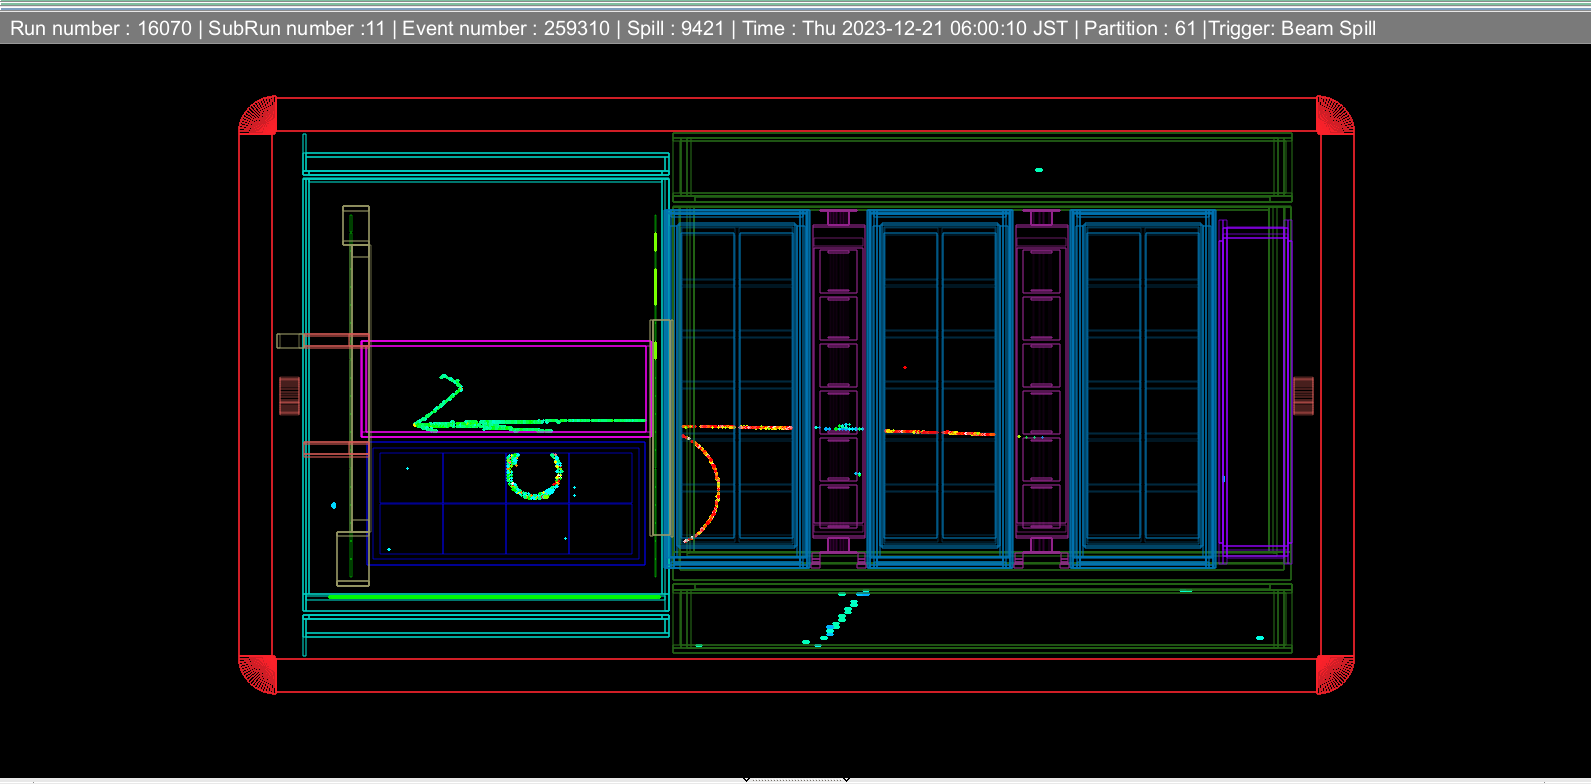
\includegraphics[width=0.5\linewidth]{fig/upgradeEvtDis.png}
        \caption{Event display of a possible $\pi^+$ event.}
        \label{fig:ndup-evedis}
    \end{figure}
\begin{savequote}[8cm]
Leider kann ich nicht persoenlich in Tuebingen ercscheinen, \\
da ich infolge eines in der Nacht vom 6. zum 7 Des. in Zuerich stattfindenden Balles hier unabkoemmlich bin.

  Unfortunately, I cannot personally appear in Tübingen since I am indispensable here in Zürich \\ because of a ball on the night from December 6 to 7.
  \qauthor{--- Wolfgang Pauli~\cite{Pauli:1930pc}, translation: Kurt Riesselmann}

\end{savequote}

\chapter{\label{ch:nu-hist}The History of Neutrinos}
\minitoc

The field of neutrino physics is relatively young and has developed rapidly over the years.
This chapter will go back in time to the birth of neutrino physics and note some of the important milestones.
As this only serves as a prologue to the thesis, it is by no means a complete historical account.
Let us dive into the fruitful history of the field.

\section{The Past}
The field of neutrino physics has a dramatic opening that many know of—in a letter~\cite{Pauli:1930pc} from Wolfgang Pauli to the Radioactivity Conference in 1930, which he did not attend in person as he was indispensable at a ball in Zuerich. 
The letter proposed a solution to the then very puzzling problem of $\beta$ decay.
It was thought of as a two-body decay, where the heavier nucleus decays to a lighter nucleus and an electron, which carries away a well-defined amount of energy due to the mass difference between the parent and daughter nucleus.  
However, the measured electron energy spectrum was a wide distribution rather than the fixed value expected. 
In his letter, Pauli postulated a third, but undetected, particle in the decay that shared the energy budget with the electron so that the sum of the third particle's energy and the electron's energy is equal to the fixed value expected, but not the electron energy alone. 
Originally, he coined this particle the ``neutron'', but this name did not stick and was given to the now-known neutron discovered by James Chadwick in 1932.
The present name, ``neutrino'', was later coined by Edoardo Amaldi in a conversation with Enrico Fermi, who later published the seminal paper on his theory of beta decay in 1934~\cite{Fermi:1934hr}, laying the theoretical foundation for subsequent experimental work.
However, the cross-section for neutrino interaction is estimated to be so small, making it extremely difficult to detect.
Even Pauli lamented, ``I have done a terrible thing. I have postulated a particle that cannot be detected.''

It was such a formidable task that Frederick Reines even proposed using the atomic bomb as the neutrino source to have an intense source of neutrinos for detection.
Fortunately, Reines and his collaborator, Clyde Cowan, discovered that the delay between the signal of neutron capture and the signal of annihilation between electron and positron, the product of the antineutrino interaction, is distinct and could be utilised to significantly reduce backgrounds, allowing a less intense (and less dangerous) source of antineutrinos to be used.
It was not until about 26 years after the postulation of the neutrino that it was directly detected in the Cowan-Reines experiment at the Savannah River Plant in 1956~\cite{Cowan:1956rrn}. 
The detector was mainly composed of $1400$ litres of liquid scintillator and $200$ litres of cadmium-loaded water as target and neutron capturer.
This remarkable achievement was recognised with a Nobel Prize in 1995.

After the Cowan-Reines experiment, the existence of the neutrino was beyond doubt, and the field of neutrino physics developed rapidly. 

There were two naturally complementary directions for development.
One was to build larger and more advanced detectors to measure the existing neutrino sources, for example, solar neutrinos, reactor neutrinos, atmospheric neutrinos, and others.
The other was to include neutrino production as part of the experiment, which became the field of accelerator neutrinos.

Roughly about the same time, Raymond Davis was also working at the Savannah River Plant, using the inverse beta decay of chlorine to argon, suggested by Pontecorvo~\cite{Pontecorvo:1946mv}, to detect neutrinos.
His experiment measured a $20$ times smaller cross-section for antineutrinos than for neutrinos in the inverse beta decay turning chlorine into argon, providing evidence for neutrinos and antineutrinos being different particles~\cite{Davis:1959pba}.
Later, he applied the same technique to measure the solar neutrino flux with a detector of the size of $378,000$ litres at the Homestake Mine~\cite{Davis:1964zz}, sufficient to detect solar neutrinos based on the Standard Solar Model calculation done by John Bahcall~\cite{Bahcall:1964ya}.
It was to everyone's surprise that the Homestake experiment only observed about one-third of the expected flux~\cite{Davis:1968}, a discrepancy known as the solar neutrino problem.
Davis and Bahcall did meticulous checks on their results and found no errors large enough to explain the discrepancy.
This phenomenon sparked many efforts, both experimentally and theoretically, to resolve the observed discrepancy.
The idea of neutrino oscillation was actually proposed even before the solar neutrino problem by Pontecorvo in 1957~\cite{Pontecorvo:1957qd} and completed by Maki, Nakagawa, and Sakata in 1962~\cite{Maki:1962mu}.
However, it was just one of the possible solutions back then among many other theories.
Papers on the other piece of the solution, the MSW effect, were published in the 1980s.
The combined solution, the large-mixing-angle MSW solution, provided an attractive answer to the solar neutrino problem.
Subsequent experiments, such as Kamiokande, a $3,000,000$-litre water Cherenkov experiment led by Masatoshi Koshiba~\cite{Kamiokande-II:1989hkh}, GALLEX~\cite{GALLEX:1998kcz}, and SAGE~\cite{SAGE:1999nng}, confirmed the solar neutrino deficit.
The definitive evidence came in 2001, when the Sudbury Neutrino Observatory (SNO) experiment, with a $1,000,000$-litre heavy water Cherenkov detector, published its result~\cite{SNO:2001kpb}, directly showing that the observed deficit of electron neutrinos was due to oscillation into other flavours.
The following year, Davis and Koshiba promptly received a Nobel Prize in Physics.
Meanwhile, in 1998, the upgrade of Kamiokande, the Super-Kamiokande ($50,000,000$-tonne water Cherenkov detector), reported the observation of neutrino oscillation in atmospheric neutrinos~\cite{Super-Kamiokande:1998kpq}.
Takaaki Kajita (Super-Kamiokande) and Arthur McDonald (SNO) shared a Nobel Prize for their work on neutrino oscillation in 2015.

Along the other development route, Pontecorvo suggested the possibility of using accelerated protons hitting targets to produce mesons that decay to produce a beam of neutrinos in 1959~\cite{Pontecorvo:1959sn}.
A year later, a similar proposal was made independently by Mark Schwartz~\cite{Schwartz:1960hg} to use accelerator-produced neutrinos to address another puzzle at that time, whether the muon neutrino is the same as the electron neutrino.
Schwartz and his collaborators, which included Leon Lederman and Jack Steinberger, used the Alternating Gradient Synchrotron at the Brookhaven National Laboratory to perform the first accelerator neutrino beam.
The neutrino interaction was recorded by a $10$-tonne spark chamber, which was able to reconstruct clear muon tracks from the interaction.
In 1962, the collected data proved that muon neutrinos are distinct from electron neutrinos~\cite{Danby:1962nd}.
Schwartz, Lederman, and Steinberger were awarded the Nobel Prize in 1988.
For the subsequent decades, accelerator neutrinos were used to help progress the more general field of particle physics due to the unique nature of neutrino scattering.
For instance, neutral current interaction was first observed by the Gargamelle bubble chamber at CERN using a beam of neutrinos~\cite{GargamelleNeutrino:1973jyy}.
High-energy neutrino beams were also deployed to test the electroweak theory and study the nucleon structure by the CDHS experiment at CERN~\cite{Schlatter:2015nxk}.

The field has entered a phase of precision measurement that will be illustrated in the next subsection.
The two complementary development routes in the past have combined in long-baseline experiments to elucidate the few remaining questions in the field.

% To better appreciate the historical progress of neutrino physics, it is clearer to put it in the perspective of the overall development of particle physics.

% Electron was discovered by J.J. Thomson in 1897.
% Proton was discovered by Rutherford in 1917.
% Neutron was discovered by Chadwick in 1932.
% Paul Dirac published the famous Dirac equation in 1928, predicting the existence of the positron, the anti-particle of the electron, which was discovered by Carl Anderson in 1932.
% Beta decay was discovered by Lise Meitner and Otto Hahn in 1938 to be a weak interaction process, where a neutron decays to a proton, an electron and an anti-neutrino.
% The muon was discovered by Carl Anderson in 1936, which was initially thought to be the Yukawa particle responsible for the strong nuclear force.

% ``Weak interaction'' is first coined by Enrico Fermi in 1933 to describe the force responsible for beta decay. <CHECK>
% On the theoretical front, Fermi proposed a theoretical solution to the beta decay in 1934.

% In 1954, CN Yang and Robert Mills published the seminal paper on non-abelian gauge theory, laying the foundation for the Standard Model.
% In 1960s and 1970s, rapid progress was made in the unifications of the electromagnetic and weak interactions, leading to the Glashow-Salam-Weinberg (GSW) model, who shared the Nobel Prize in Physics in 1979. 
% The discovery of the W and Z bosons at CERN in 1983.

% It was suggested by Markov [65], Pontecorvo [66], and Schwartz [67] to use proton accelerators to produce high energy
% neutrino beam from pion decays to perform experiments like:
% nu+n->mu+n
% etc
% The experiments performed at the Brookhaven National Laboratory (BNL) by Danby et al. [71] and later at
% CERN by Bienlein et al. [72] 
% observed only muon but never elec tron, confirming numu and nue are different (1962)

% 1965 BNL introducted the POT idea as a measure of the neutrino flux

% Tau in 1975
% the existence of a new flavor of
% neutrinos ντ was proposed, which was observed much later in the DONUT experiment [74,75] in 2000 at the Fermilab

% It was Fermi [3,4] and Perrin [5] who first discussed the determination of the neutrino mass from the study of the end-point spectrum of beta decay.

\section{The Present}
With neutrino oscillation finally confirmed, the field of neutrino physics has a fruitful past and a clear theoretical framework laid out.
The present task for the field is the precise measurement of the parameters in the theoretical framework, namely the neutrino masses and the PMNS matrix elements.
The measurements given in this section follow from the latest Particle Data Group release~\cite{ParticleDataGroup:2024cfk}.

The mass of the electron neutrino can be studied by investigating the shape of the high-energy tail of the electron spectrum in tritium beta decay, a method proposed in Fermi's theory paper on $\beta$-decay~\cite{Fermi:1934hr} and independently by Francis Perrin~\cite{Perrin1933}.
The KATRIN experiment employs this method and produces one of the most stringent upper bounds, $0.8~\ev$ with $90\%$ confidence level~\cite{KATRIN:2021uub}.
There are other methods to extract the neutrino mass, such as from cosmological observations~\cite{Brieden:2022lsd}, but as this thesis focuses on neutrino oscillation, these will not be elaborated for conciseness.

As neutrino oscillation depends on the mass difference squared as well, oscillation experiments are able to measure the neutrino masses indirectly through the mass differences in addition to the PMNS matrix elements.
Contrary to the electron neutrino mass measured from $\beta$-decay, the mass differences measured in oscillation experiments are the differences between the neutrino mass eigenstates.
The general structure of the mass eigenstates is that there is a small difference between $m_2$ and $m_1$, but $m_3$ is either much smaller or larger than $m_2$ and $m_1$.
The relation between $m_3$ and the others is the mass hierarchy problem.
The case where $m_3$ is the largest is called the Normal Ordering (NO), and the case where $m_3$ is the smallest is the Inverted Ordering (IO).
The KamLAND collaboration performed a global fit of data sets across several types of neutrino experiments in 2013, leading to the measurement of $\delmtwoo=7.53\pm0.18~\times 10^{-5}~\ev$~\cite{KamLAND:2013rgu}.
Note that this difference is not the absolute value as it is known that $m_2>m_1$.
As for $\delmthro$, the estimation is produced from a global fit of accelerator, reactor, and atmospheric data by PDG, giving $\delmthro=2.455^\pm0.028~\times 10^{-3}~\ev^2$ (NO) and $\delmthro=-2.455^\pm0.028~\times 10^{-3}~\ev^2$ (IO).

The specific meaning of the parameters in the PMNS matrix will be illustrated later in Sec.~\ref{sec:oscillaltion}, while the respective measurements are first given here without breaking the flow.
The PMNS matrix can be parameterised by three mixing angles, namely $\totwo$, $\tothr$ and $\ttthr$, and a CP violation phase, $\dcp$.
The current best estimate of $\totwo$ is given by a fit of the KamLAND measurement and solar measurements in 2016, producing $\sin^2(\totwo)=0.307^{+0.013}_{-0.012}$.
The estimation of $\ttthr$ is done by the PDG using accelerator and atmospheric neutrino data~\cite{ParticleDataGroup:2024cfk}, leading to $\sin^2(\ttthr)=0.553^{+0.016}_{-0.024}$ (IO) and $\sin^2(\ttthr)=0.558^{+0.015}_{-0.021}$ (NO).
The last mixing angle, the average of $\tothr$, is obtained by PDG using accelerator and reactor data, giving $\sin^2(\tothr)=2.19\pm0.07$.
The last parameter, $\dcp$, is the least well measured.
The PDG average of existing accelerator and atmospheric data gives $\dcp=1.19\pm0.22$ in radians.

From being completely unknown to precisely measured, neutrino oscillation is now a well-understood phenomenon except for the mass ordering and the extent of CP violation, which is the pressing goal of the present and future LBL neutrino experiments.
 
\section{The Plans}
To elucidate the remaining questions in neutrino physics, new experiments are planned or under construction and existing experiments are undergoing upgrades.
This sub-section will only briefly describe some of them and it is not meant to be an exhaustive review.

The successor of the Daya Bay experiment, which produced one of the most precise measurements of $\tothr$, the Jiangmen Underground Neutrino Observatory (JUNO), is set to start operation in summer 2025~\cite{ScienceNews2025}.
Located near the Yangjiang and Taishan nuclear power plants, JUNO has a $20,000$-tonne liquid scintillator.
It is projected to determine the mass ordering with $3~(3.1)\sigma$ significance for NO (IO) in $6.7$ years of data taking~\cite{Paoloni:2024atc}.

The successor of the Super-K experiment, the Hyper-Kamiokande (Hyper-K)~\cite{Hyper-Kamiokande:2018ofw}, is under construction and is expected to operate in 2027.
Hyper-K is a $258,000$-ton water Cherenkov detector, about $8$ times the size of its predecessor, Super-K.
It uses the same beamline as the T2K experiment and measures the electron neutrino appearance to determine $\dcp$.
With $10$ years of data taking, it is projected to exclude CP conservation to $5\sigma$ for more than $60\%$ of true $\dcp$ values and to $3\sigma$ for $75\%$ of $\delta_{CP}$ values assuming the systematic uncertainties are controlled at $2.7\%$~\cite{Jesus-Valls:2024ady}.

Another large-scale LBL neutrino experiment is the Deep Underground Neutrino Experiment (DUNE)~\cite{DUNE:2016hlj,DUNE:2015lol,DUNE:2016evb,DUNE:2016rla,DUNE:2021tad}.
Its far detector consists of four $17,000$-ton Liquid Argon Time Projection Chambers (LArTPC) and it has a beamline of $1300$~km, which enables it to be highly sensitive to the mass ordering as well.
With the novel LArTPC technology, it is expected to reach $5\sigma$ for the mass ordering with 3 years of data taking and reach $3\sigma$ for $75~\%$ of $\delta_{CP}$ values with about 15 years of data taking~\cite{Gil-Botella:2024duf}.
There is no clear estimation of the starting time for DUNE yet, but the test experiment for its far detector, the ProtoDUNE experiment, has operated for more than 2 years at CERN.

In the projected sensitivity of these future experiments, the importance of reducing systematic uncertainties cannot be over-emphasised as results obtainable with years of data taking would need decades instead if the systematic uncertainties do not reach the required level.
This is exactly why T2K is upgrading its near detector to better understand neutrino interactions to reduce systematics, which is exactly what this thesis is about.

Besides the measurement of the known parameters, there are also a plethora of beyond the Standard Model searches both at existing and future experiments.
Moreover, there has been impressive progress on utilising neutrinos for cosmological observation by experiments, such as IceCUBE.
Although they are not elaborated in this thesis, they represent the highly exciting development of the field.
From the $1400$-litre liquid scintillator detector in the Cowan-Reines experiment to the $1,000,000$-litre heavy water Cherenkov detector of SNO and to the $258,000,000$-litre water Cherenkov detector of Hyper-K, the field of neutrino physics has grown rapidly.
From being the most elusive particle, which was thought never possible to detect, to a sophisticated understanding of neutrino oscillation, our understanding of the properties of neutrinos has improved drastically.
With the incredible experiments in plan and running, it is promising that a definitive measurement of all the neutrino properties is reachable, and its results will be profound and shed light on new physics directions.

\begin{savequote}[8cm]
Well, you shouldn’t believe
everything you read in the papers.

  \qauthor{--- Hans Bethe \textit{F. Reienes, Nobel Lecture 1995}}

\end{savequote}

\chapter{\label{ch:nu-theo}The Theory of Neutrinos}
\minitoc
The main goal of neutrino experiments is to measure all neutrino properties, including the mass, mixing angles, and the CP violation parameter, $\dcp$. 
The mixing angles and $\dcp$ fully describes neutrino oscillation, while the mass is the reason why neutrino oscillation occurs.
Hence, these parameters will be better illustrated in Sec.~\ref{sec:oscillation} in the context of the theoretical framework of neutrino oscillation.
As only products from neutrino interactions are detected in experiments, achieving this goal requires a good understanding of neutrino interactions.
Hence, a brief overview of neutrino interactions is given in Sec.~\ref{sec:interaction}.

\section{Oscillation}
\label{sec:oscillation}
Neutrinos come in three flavours: the electron neutrino ($\nu_e$), the muon neutrino ($\nu_\mu$), and the tau neutrino ($\nu_\tau$).
The different flavours of neutrinos will only produce the corresponding lepton in weak interactions, so they are eigenstates of the weak interaction.
However, neutrinos propagate through space as mass eigenstates, $\nu_1$, $\nu_2$, and $\nu_3$.
The reason for neutrino oscillation to occur is twofold.
One is because the mass eigenstates do not have a simple one-to-one correspondence with the weak eigenstates. 
They are superpositions of the weak eigenstates.
The other reason is that these mass eigenstates have different masses.
Neutrinos are created as flavour eigenstates in weak interactions, but they propagate as a linear combination of mass eigenstates, which propagate with different phase velocities due to their different masses.
Hence, throughout the propagation, the linear combination of mass eigenstates continually changes, leading to a varying superposition of flavour eigenstates, and thus, neutrino oscillation.

To be more specific, the matrix describing the mixing of mass eigenstates into flavour eigenstates is the PMNS matrix.
It is conventionally parametrised as 
\begin{equation}
U_{\text{PMNS}} = 
\begin{pmatrix}
1 & 0 & 0 \\
0 & c_{23} & s_{23} \\
0 & -s_{23} & c_{23}
\end{pmatrix}
\begin{pmatrix}
c_{13} & 0 & s_{13} e^{-i\dcp} \\
0 & 1 & 0 \\
-s_{13} e^{i\dcp} & 0 & c_{13}
\end{pmatrix}
\begin{pmatrix}
c_{12} & s_{12} & 0 \\
-s_{12} & c_{12} & 0 \\
0 & 0 & 1
\end{pmatrix},
\end{equation}
where $c_{ij} = \cos\theta_{ij}$ and $s_{ij} = \sin\theta_{ij}$, and $\dcp$ is the CP violation phase.
The angles $\theta_{ij}$ are the mixing angles. 
Using the PMNS matrix, the flavour eigenstates can be expressed in terms of the mass eigenstates as 
\begin{equation}
\begin{pmatrix}
\nu_e \\
\nu_\mu \\
\nu_\tau
\end{pmatrix}
=
U_{\text{PMNS}}
\begin{pmatrix}
\nu_1 \\
\nu_2 \\
\nu_3
\end{pmatrix}.
\end{equation}
The derivations of the following results can be obtained readily with pen and paper, so 
to keep a close focus on the development of the theoretical idea, detailed derivations are not included here. 
Due to the small neutrino masses, a mass eigenstate with mass $m_i$ acquires the following phase approximately:
\begin{equation}
  \ket{\nu_i(L)} = e^{-i \frac{m_i^2 L}{2E}} \ket{\nu_i(0)},
\end{equation}
after travelling a distance $L$ with energy $E$.
Hence, the probability that a neutrino of flavour $\alpha$ created at the source is detected as a neutrino of flavour $\beta$ after travelling a distance $L$ is given by
\begin{align}
  P_{(\alpha \to \beta)} &= \left|\braket{\nu_\beta | \nu_\alpha(L)} \right|^2 = \left| \sum_i U_{\alpha i} U^*_{\beta i} e^{-i \frac{m_i^2 L}{2E}} \right|^2 \\
  &= \delta_{\alpha\beta} - 4 \sum_{i>j} \text{Re} \bigl( U_{\alpha i} U^*_{\beta i} U^*_{\alpha j} U_{\beta j} \bigr) \,\sin^2 \!\Bigl( \frac{\Delta m^2_{ij} L}{4E} \Bigr) \\
  &\quad + 2 \sum_{i>j} \text{Im} \bigl( U_{\alpha i} U^*_{\beta i} U^*_{\alpha j} U_{\beta j} \bigr) \,\sin \!\Bigl( \frac{\Delta m^2_{ij} L}{2E} \Bigr),
\end{align}
where $\delta_{\alpha\beta}$ is the Kronecker delta, $U_{\alpha i}$ is the element of the PMNS matrix, and $\Delta m^2_{ij} = m_i^2 - m_j^2$.
This result shows that the oscillation probability depends on the mixing angle through the PMNS matrix elements and on the mass difference and neutrino energy through the sine terms.
For brevity, the dependence on the sine terms can be characterised by a phase angle,
\begin{equation}
  \label{eq:osc-phase}
  \Delta_{ij} = \frac{\Delta m^2_{ij} L}{2E} \approx 1.27 \frac{\Delta m^2_{ij} [\text{eV}^2] L [\text{km}]}{E [\text{GeV}]},
\end{equation}
where the oscillation is maximal when $\Delta_{ij} = \pi / 2$.
These results can be used to better understand how the various parameters are measured in different types of neutrino experiments.
The different sensitivities of these experiments arise from the relatively large differences in both the mixing angles and the mass differences.
The latest values for the neutrino parameters based on Ref.~\cite{Capozzi:2021fjo,ParticleDataGroup:2024cfk} are provided in Table~\ref{tab:neutrino-parameters}, which shows that the magnitude of $\delmtwoo$ is much smaller than that of $\delmthro$.
Unlike the CKM matrix, where all mixing angles are small, only $\theta_{13}$ is small here, while the other two angles are considerably larger, giving rise to significant mixing.

\begin{table}[h]
  \centering
  \begin{tabular}{c|c|c}
    Parameter & Value & Sensitive Experiment\\
    \hline
    \hline
    $\Delta m^2_{21}~(\text{eV}^2)$ & $7.36^{+0.16}_{-0.15} \times 10^{-5}$ & Reactor and solar \\
    $|\Delta m^2_{31}|~(\ev^2)$ & $2.448^{+0.023}_{-0.031} \times 10^{-3}$ & Atmospheric \\
    $\theta_{12}$ ($^\circ$) & $33.40^{+0.80}_{-0.82}$ & Reactor and solar \\
    $\theta_{23}$ ($^\circ$)       & $42.4^{+1.0}_{-0.9}$ & Atmospheric\\
    $\theta_{13}$ ($^\circ$)       & $8.59^{+0.13}_{-0.12}$ & Reactor and solar \\
    $\dcp$ ($^\circ$) & $223^{+32}_{-23}$   & Accelerator and atmospheric \\
    \hline
  \end{tabular}
  \caption{The latest values for the neutrino parameters.}
  \label{tab:neutrino-parameters}
\end{table}

\subsection{Atmospheric neutrinos}
Atmospheric neutrinos are mostly muon neutrinos produced from the decay of mesons created by cosmic rays interacting with the atmosphere.
The neutrino energy is typically of the order of $1~\gev$, while the distance travelled ranges from $O(10^2)$ to $O(10^4)~\km$.
Substituting these numbers into Eq.~\ref{eq:osc-phase}, $\Delta_{23}$ is of the order of $O(10^{-2})$ to $O(1)$, whereas $\Delta_{21}$ is of the order of $O(10^{-3})$ to $O(10^{-1})$.
Hence, oscillation is much more prominent in the $\nu_\mu \to \nu_\tau$ channel than in the $\nu_\mu \to \nu_e$ channel.
This is why atmospheric neutrino experiments are sensitive to $\theta_{23}$ and $\Delta m^2_{32}$, sometimes referred to as the atmospheric mixing angle and mass difference, respectively.

\subsection{Reactor neutrinos}
Reactor neutrinos are mostly electron antineutrinos produced from nuclear fission in power plants.
Their energy is typically of the order of $1~\mev$.
Unlike atmospheric neutrino measurements, detectors can be placed at various locations to measure different parameters.
Thus, it is more convenient to discuss reactor neutrino oscillation by introducing the oscillation length variable given as:
\begin{equation}
  \label{eq:osc-length}
  L_{\text{osc}} = \frac{4\pi E}{\Delta m^2} = 2.48 \frac{E [\text{MeV}]}{\Delta m^2 [\text{eV}^2]} \text{m},
\end{equation}
which corresponds to one complete period of neutrino oscillation.
Substituting the reactor neutrino energy into Eq.~\ref{eq:osc-length}, one obtains $L_{\text{osc}} = O(10^2)~\km$ for $\delmtwoo$ and $L_{\text{osc}} = O(1)~\km$ for $\delmthro$. 
Hence, by placing detectors kilometres away from the power plants, reactor neutrino experiments offer the unique opportunity to measure $\theta_{13}$ and $\delmthro$, sometimes referred to as the reactor mixing angle and mass difference, respectively.
Additionally, placing detectors at about $O(100)~\km$ from the power plants allows measurements of $\delmtwoo$.

\subsection{Solar neutrinos}
Solar neutrinos are mostly electron neutrinos produced from nuclear fusion in the Sun.
Most solar neutrinos have energies below $1~\mev$, except those from $^8$B decay, which can reach $15~\mev$.
The distance travelled by solar neutrinos is of the order of $O(10^8)~\km$.
Substituting these values into Eq.~\ref{eq:osc-length}, one obtains $L_{\text{osc}} = O(10^4)~\m$ for $\delmtwoo$ and $L_{\text{osc}} = O(10^3)~\m$ for $\delmthro$.
Both are much smaller than the average distance travelled, so observing the clear oscillatory pattern (as in other neutrino experiments) would require knowing each neutrino’s travel distance and starting position with extremely high precision, which is beyond current detection capabilities.
Fortunately, the average oscillation result can still be measured by the total survival rate of electron neutrinos.

Beyond the usual neutrino oscillation, there is another important phenomenon in solar neutrino measurements: the Mikheyev–Smirnov–Wolfenstein (MSW) matter effect~\cite{Wolfenstein:1977ue,Mikheyev:1985zog}.
A detailed discussion of the MSW effect is beyond the scope of this thesis.
In short, the MSW effect modifies the mixing parameters due to the presence of electrons in matter.
This modification can enhance or suppress the oscillation probability depending on the mass difference and the electron density.
Roughly speaking, the required electron density is proportional to the mass difference squared and inversely proportional to the neutrino energy.
Hence, lower neutrino energy or a larger mass difference necessitates a higher electron density to modify the oscillation probability.
Because $\delmthro$ is considerably larger, for nearly all solar neutrino energies, the electron density in the Sun is insufficient to modify the mixing between $\nu_1$ and $\nu_3$ significantly.
As for the relatively smaller $\delmtwoo$, the electron density is high enough to substantially modify the mixing between $\nu_1$ and $\nu_2$ for the high-energy neutrinos from $^8$B decay.
The outcome for these high-energy electron neutrinos is a rearrangement of their mass-eigenstate composition such that, upon leaving the Sun’s surface, they are mostly $\nu_2$, a considerably greater fraction than in the unmodified scenario for the low-energy electron neutrinos.
The MSW effect is seen when different experiments measure solar neutrinos at different energies and observe varying electron-neutrino survival rates.
Hence, the absolute survival rates are particularly sensitive to $\theta_{12}$, which is often referred to as the solar mixing angle. 

\subsection{Accelerator neutrinos}
In accelerator neutrino experiments, there is relatively greater flexibility than in other types of neutrino experiments because both the neutrino source and the detector can be designed to optimise oscillation studies.
This section uses T2K as an example, but the underlying principles apply to all LBL experiments.
More details about the T2K experiment are presented in Chapter~\ref{ch:t2k}.

Neutrinos are produced in accelerators by bombarding protons onto a target (carbon in T2K), creating numerous mesons.
The charged mesons can be steered to point in the required direction using sophisticated magnetic horns.
Besides directionality, the magnetic horns can also select mesons of a desired charge.
For instance, positive (negative) pions can be focused if a beam of muon (anti)neutrinos is needed.
It is this control over the neutrino source that enables accelerator experiments to measure $\delta_{CP}$.
Since the neutrino energy from meson decay depends on the emission angle, varying the angle between the detector and the beam direction yields different energy distributions.
T2K places its detectors $2.5^\circ$ off-axis to obtain a neutrino beam with a narrow energy peak at about $0.6~\gev$.
According to Eq.~\ref{eq:osc-phase}, for maximal oscillation with the larger mass difference (i.e.\ $\delmthro \approx 2.5 \times 10^{-3}~\ev^2$), the far detector should be placed around $300$~km from the source.
Hence, accelerator measurements are sensitive to $\theta_{13}$.
Furthermore, by analysing muon neutrino disappearance, accelerator experiments can also measure $\theta_{23}$ and $\delmthrt$.
By analysing oscillations in neutrino and antineutrino modes, T2K can extract a best-fit value of $\delta_{CP}$ that describes the observed data~\cite{T2K:2019bcf}.
However, the current measurement is severely limited by statistics and thus suffers large uncertainties.
Due to the significant increase in the fiducial volume of Hyper-K, statistics are expected to increase significantly, and reducing systematic uncertainties proportionally will be paramount for fully exploiting that potential.
This leads naturally to the discussion of one of the major sources of systematic uncertainty in neutrino experiments: neutrino interactions.

\section{Interaction}
\label{sec:interaction}
The underlying theory for neutrino oscillation is straightforward, and the parameters to be measured are clear, but the experimental determination of these parameters is challenging.
Due to the weak interaction of neutrinos, they cannot be detected directly.
All neutrino measurements are based on detecting the particles produced in neutrino interactions.
Hence, to extract the desired neutrino oscillation parameters with high precision, a good understanding of neutrino interactions is crucial.
This chapter provides the basic understanding of neutrino interactions necessary for interpreting the analyses presented in the subsequent chapters.

\subsection{$\nu$-quark}
The most fundamental interaction between a neutrino and matter is the weak interaction between the neutrino and a quark, whose Feynman diagrams are shown in Fig.~\ref{fig:nu-q-feyn}.

\begin{figure}[h]
  \centering
  \begin{subfigure}[b]{0.45\textwidth}
    \centering
    \begin{tikzpicture}
      \begin{feynman}
        \vertex (a) {\(\nu_\ell\)};
        \vertex [right=of a] (b);
        \vertex [right=of b] (c) {\(\ell\)};
        \vertex [below=of b] (d);
        \vertex [left=of d] (e) {\(q\)};
        \vertex [right=of d] (f) {\(q'\)};
        
        \diagram* {
          (a) -- [fermion] (b) -- [fermion] (c),
          (b) -- [boson, edge label=\(W\)] (d),
          (e) -- [fermion] (d) -- [fermion] (f),
        };
      \end{feynman}
    \end{tikzpicture}
    \caption{Charge current interaction.}
    \label{fig:cc-interaction}
  \end{subfigure}
  \hfill
  \begin{subfigure}[b]{0.45\textwidth}
    \centering
    \begin{tikzpicture}
      \begin{feynman}
        \vertex (a) {\(\nu_\ell\)};
        \vertex [right=of a] (b);
        \vertex [right=of b] (c) {\(\nu_\ell\)};
        \vertex [below=of b] (d);
        \vertex [left=of d] (e) {\(q\)};
        \vertex [right=of d] (f) {\(q\)};
        
        \diagram* {
          (a) -- [fermion] (b) -- [fermion] (c),
          (b) -- [boson, edge label=\(Z\)] (d),
          (e) -- [fermion] (d) -- [fermion] (f),
        };
      \end{feynman}
    \end{tikzpicture}
    \caption{Neutral current interaction.}
    \label{fig:nc-interaction}
  \end{subfigure}
  \caption{Feynman diagrams for neutrino interactions with a quark.}
  \label{fig:nu-q-feyn}
\end{figure}
More specifically, the interaction shown in Fig.~\ref{fig:cc-interaction} is mediated by the $W$ boson, and the neutrino is converted into a charged lepton, while Fig.~\ref{fig:nc-interaction} is mediated by the $Z$ boson, and the neutrino remains a neutrino.
The former is the charged current (CC) interaction, while the latter is the neutral current (NC) interaction.
Following the Feynman diagram, it is straightforward to write down the amplitude for the interaction.
The amplitude for the CC interaction is given by:
\begin{equation}
  \mathcal{M}_{\text{CC}} = \frac{g^2}{2} \bar{u}_\ell(p') \gamma^\mu (1 - \gamma^5) u_\nu(p) \frac{-i g_{\mu\nu}}{q^2 - M_W^2} \bar{u}_q(k') \gamma^\nu (1 - \gamma^5) u_q(k),
\end{equation}
where $g$ is the weak coupling constant, $u_\ell$ and $u_\nu$ are the spinors for the outgoing lepton and incoming neutrino respectively, $u_q$ are the spinors for the quarks, $q$ is the momentum transfer, and $M_W$ is the mass of the $W$ boson.
Due to confinement, this interaction does not occur freely in nature.
Instead, this interaction occurs only when the neutrino has sufficiently high energy to probe inside the nucleon and interact with the quarks.
The product quark will hadronise, producing a jet of particles.
This type of interaction is referred to as deep inelastic scattering (DIS).
DIS is highly complicated and not so relevant for this thesis, so it will not be discussed further.
More details can be found in reviews such as Ref.~\cite{SajjadAthar:2022pjt}.

\subsection{$\nu$-nucleon}
At the T2K beam energy, most neutrinos do not have enough energy to probe within the nucleon but rather interact with the nucleon as a whole.
Depending on the specific neutrino energy, the interaction can be classified as quasi-elastic (QE), resonance, or deep inelastic scattering (DIS).

\subsubsection{QE}
Although at the quark level the interaction appears the same as in Fig.~\ref{fig:nu-q-feyn}, the interacted quark cannot be treated as independent but rather as part of a nucleon.
Hence, the effective $\nu$-nucleon interaction Feynman diagram is shown in Fig.~\ref{fig:nu-n-feyn}.

\begin{figure}[h]
  \centering
  \begin{subfigure}[b]{0.45\textwidth}
    \centering
    \begin{tikzpicture}
      \begin{feynman}
        \vertex (a) {\(\nu_\ell\)};
        \vertex [right=of a] (b);
        \vertex [right=of b] (c) {\(\ell\)};
        \vertex [below=of b] (d);
        \vertex [left=of d] (e) {\(N\)};
        \vertex [right=of d] (f) {\(N'\)};
        
        \diagram* {
          (a) -- [fermion] (b) -- [fermion] (c),
          (b) -- [boson, edge label=\(W\)] (d),
          (e) -- [fermion] (d) -- [fermion] (f),
        };
      \end{feynman}
    \end{tikzpicture}
    \caption{Charge current interaction.}
    \label{fig:cc-interaction-n}
  \end{subfigure}
  \hfill
  \begin{subfigure}[b]{0.45\textwidth}
    \centering
    \begin{tikzpicture}
      \begin{feynman}
        \vertex (a) {\(\nu_\ell\)};
        \vertex [right=of a] (b);
        \vertex [right=of b] (c) {\(\nu_\ell\)};
        \vertex [below=of b] (d);
        \vertex [left=of d] (e) {\(N\)};
        \vertex [right=of d] (f) {\(N\)};
        
        \diagram* {
          (a) -- [fermion] (b) -- [fermion] (c),
          (b) -- [boson, edge label=\(Z\)] (d),
          (e) -- [fermion] (d) -- [fermion] (f),
        };
      \end{feynman}
    \end{tikzpicture}
    \caption{Neutral current interaction.}
    \label{fig:nc-interaction-n}
  \end{subfigure}
  \caption{Feynman diagrams for neutrino interactions with a nucleon.}
  \label{fig:nu-n-feyn}
\end{figure}
The leptonic current remains the same, but the hadronic current is now a nucleon current instead of a quark current.
Hence, the hadronic current is much more complicated, comprising several form factors that parametrise our understanding of the nucleon structure.
For instance, the amplitude for the CC interaction in Fig.~\ref{fig:cc-interaction-n} is given by:
\begin{align}
  \mathcal{M}_{\text{CC}} =& \frac{G_F}{\sqrt{2}} \,\bar{u}_\ell(p')\,\gamma^\mu (1 - \gamma^5)\,u_\nu(p) \\
   &\times \,\bar{u}_N(k')\,\left[ F_1(q^2)\,\gamma_\mu + F_2(q^2)\,\frac{i\,\sigma_{\mu\nu}\,q^\nu}{2M} + F_A(q^2)\,\gamma_\mu\,\gamma^5 + F_P(q^2)\,\frac{q_\mu\,\gamma^5}{m_\pi} \right]\,u_N(k),
\end{align}
where $G_F$ is the Fermi constant, $M$ is the nucleon mass, $m_\pi$ is the pion mass, and the hadronic current is parametrised by the form factors, $F_1$, $F_2$, $F_A$, and $F_P$.
More details can be found in Ref.~\cite{LlewellynSmith:1978te}.
It is important to note that $F_1$ and $F_2$ are the vector form factors, which can be extracted from electron scattering measurements, and $F_P$ is the pseudoscalar form factor, which can be related to $F_A$, the axial form factor, through the Partially Conserved Axial Current (PCAC) hypothesis.
Hence, the axial form factor is unique to neutrino experiments and can only be extracted from past measurements.
Fig.~\ref{fig:cc0pi} shows an event display of a candidate $\cczpi$ event, likely a QE event, in the upgraded ND280 during the beam run in June 2024.

\begin{figure}[!htb] 	
    \centering 		
    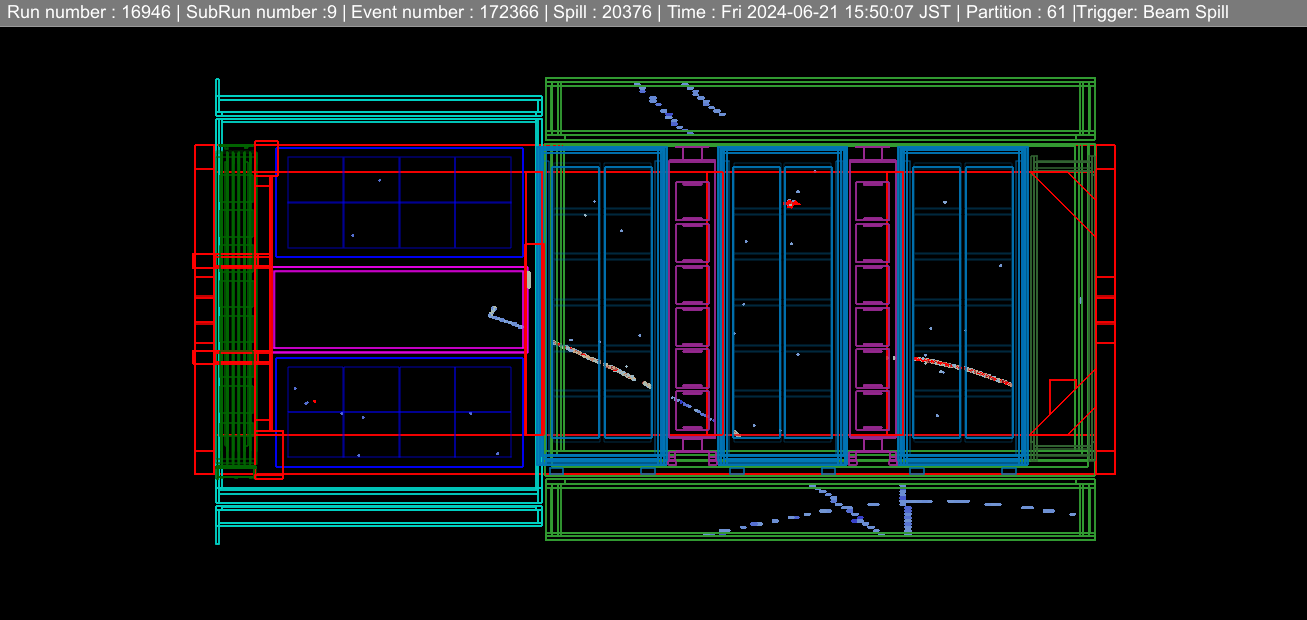
\includegraphics[width=\sgfigwid\textwidth]{figures/cc0pi.png}
    \caption{\label{fig:cc0pi} A $\cczpi$ candidate event in upgraded ND280, where the long track is the primary muon and the short track is the primary proton.} 
\end{figure}

\subsubsection{Resonance}
When the neutrino energy is high enough to excite the nucleon to a higher energy state (e.g.\ $\Delta(1232)$), the interaction is classified as a resonance interaction.
The excited nucleon decays to produce a pion. 
Hence, resonance modelling is sometimes called single pion production modelling.
One of the most common models used today is the Berger–Sehgal model, which is an improvement on the earlier Rein–Sehgal model by accounting for the effect of the lepton mass.
The Rein–Sehgal model is based on the approximate relativistic quark model in Ref.~\cite{Feynman:1971wr}.
Subsequent developments, such as the MK model~\cite{Kabirnezhad:2017jmf,Kabirnezhad:2020wtp,Kabirnezhad:2022znc}, provide more sophisticated calculations.

Fig.~\ref{fig:cc1pi} shows an event display of a candidate $\ccopi$ event, likely a resonance event, in the upgraded ND280 during the beam run in June 2024.

\begin{figure}[!htb] 	
    \centering 		
    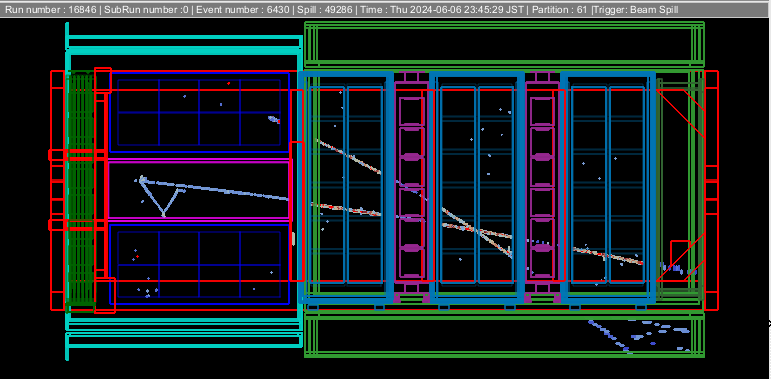
\includegraphics[width=\sgfigwid\textwidth]{figures/shortME.png}
    \caption{\label{fig:cc1pi} A $\ccopi$ candidate event in upgraded ND280, where the long track is the primary muon and the V-shaped track is identified as a pion track by the short delayed track, identified as the Michel electron, attached to its end.} 
\end{figure}

\subsection{$\nu$-nucleus}
\label{sec:nuint-nucleus}
Modern neutrino experiments use heavier elements, such as hydrocarbon and argon, to increase event rates.
This further complicates the neutrino interaction.
In the simplest case (relatively high neutrino energy), the Impulse Approximation (IA) can be applied.
The neutrino sees each nucleon as independent, so the interaction reduces to the $\nu$-N interaction.
Even in this simplest case, the presence of the nuclear medium still affects the interaction in two ways: the initial state (IS) effect and the final state interaction (FSI).

As the neutrino energy decreases, IA is no longer valid, and the nucleus can only be resolved as a whole.
In this case, Random Phase Approximation (RPA) corrections are needed.
Interested readers can refer to Ref.~\cite{SajjadAthar:2022pjt} for more details.
Instead, the two nuclear effects are elaborated below.

\subsubsection{Initial state}
Nuclear effects manifest in two ways.
Firstly, the nucleon in the interaction is in a bound state, meaning it cannot have arbitrary energy and momentum as a free nucleon would.
Instead, the nucleon’s energy distribution is parameterised by the so-called Spectral Function (SF).
The simplest form of SF is the Fermi gas model, which treats nucleons as a Fermi gas.
Hence, the nucleon momentum is filled up to the Fermi momentum, given by
\begin{equation}
    k_F = \bigl(3\pi^2 \rho/2\bigr)^{1/3},
\end{equation}
where $\rho$ is the nuclear density, approximately $2.3\times 10^{-17}~\textrm{kg}/\m^3$, leading to a Fermi momentum of about $250~\mevc$.
This model oversimplifies the nuclear structure.
A more realistic approach is the local Fermi gas (LFG) model, which accounts for the varying nuclear density.
Further improvements include short-range correlations between nucleons, which increase the fraction at high momentum~\cite{Benhar:1994hw}.

\subsubsection{Final state interactions}
\label{sec:nuint-fsi}
The second nuclear effect is the final state interactions (FSI).
Regardless of how the neutrino interacts with the nucleon, the products remain inside the nucleus and must propagate through the nuclear medium to be detected.
These interactions with the nuclear medium are classified as FSI.
They are more pronounced for hadrons than for leptons, as the latter are less likely to interact in the nuclear medium.
There are several types of FSI, including elastic scattering, charge exchange, and absorption.
\begin{enumerate}
  \item 
  Charge exchange (CEX) involves changing the charge of the participating particles; for example,
  \begin{equation}
      \pi^+ + n \rightarrow \pi^0 + p,
  \end{equation}
  or vice versa. This rescattering type is crucial for event topologies requiring the presence of a pion; depending on the signal pion’s charge, CEX could migrate events between signal and background. 

  \item 
  Inelastic scattering (INEL) is the case where the nucleus is left in an excited state after rescattering. This category applies only to situations where a single additional nucleon is emitted or knocked out after rescattering. Since it does not affect the number of pions, it will not convert a pionless topology into a pion-production topology. However, it can change the number of final-state nucleons and affect the kinematics of the leading particle.

  \item 
  Absorption (ABS) refers to processes where the pion is effectively absorbed. For instance, $\pi^+$ can interact with multiple nucleons, initially forming a baryon resonance that subsequently emits multiple nucleons rather than a pion. Thus, the $\pi^+$ no longer emerges from the nucleus.

  \item 
  Pion production (PIPD) can occur for energetic particles where an extra pion is generated through rescattering, for example:
  \begin{equation}
      p + p \rightarrow p + n + \pi^+.
  \end{equation}
  Such an interaction significantly alters the event topology, adding an extra pion.
\end{enumerate}

\subsubsection{Transverse Kinematic Imbalance}
\label{sec:nuint-tki}
Due to the heavy target nucleus in current neutrino experiments, nuclear effects are almost inextricable from conventional single-particle kinematic measurements.
This greatly impedes model development because nuclear effects can mimic different underlying $\nu$-N processes.
For instance, if the proton from a QE $\nu$-N interaction has sufficient energy to produce an additional pion during FSI, that pion may emerge from the nucleus.
Thus, a QE event could mimic resonance production.
Hence, accurate descriptions of nuclear effects are crucial to reduce model systematic uncertainties.

To gain insights into nuclear effects, observables that are sensitive to these effects must be measured.
Transverse Kinematic Imbalance (TKI) variables are exactly such observables~\cite{Lu:2015hea, Lu:2015tcr}.
The TKI variables are illustrated in Fig.~\ref{fig:stki}.

\begin{figure}[!htb] 	
    \centering 		
    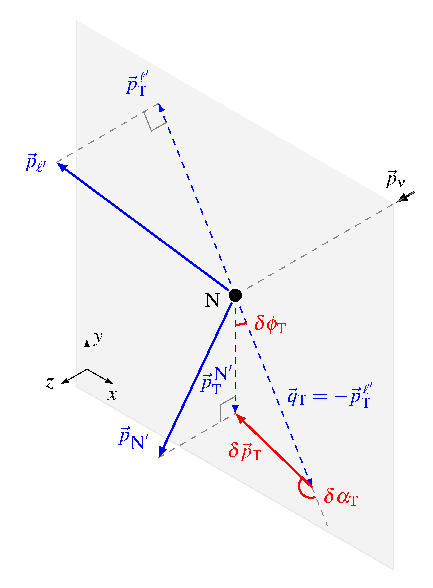
\includegraphics[width=0.35\textwidth]{figures/stki.eps}
    \caption{\label{fig:stki} Schematic illustration of the TKI variables. Diagram taken from Ref.~\cite{Lu:2015tcr}.} 
\end{figure}

In the simplest case, there are only two final particles after the neutrino–nucleon interaction: a muon and a proton. 
Without nuclear effects, these two particles should have momenta of equal magnitude but opposite direction in the plane transverse to the neutrino beam.
The TKI variables quantify the deviation from this ideal scenario, thereby probing nuclear effects. 
Because of the initial state (IS), the nucleon’s momentum distribution causes the sum of the muon and proton transverse momenta to deviate from zero, quantified by $\dpt$, and their directions need not be precisely opposite, quantified by $\dphit$.
Moreover, if the nucleus is initially at rest and no additional particles (beyond the muon and proton) are knocked out, the nucleon initial momentum $\pn$ can be estimated with an $\mathcal{O}(20\%)$ correction~\cite{Yang:2023dxk} following methods in Refs.~\cite{Furmanski:2016wqo, Lu:2019nmf}. 
Hence, $\dpt$ and $\pn$ serve as good probes of IS models.
While FSI tends to smear these distributions, the general shape and peak location mainly reflect the IS model.
Since most IS models assume no preferred direction for nucleon motion, one expects a uniform distribution in $\dat$, the angle between the initial nucleon momentum and the lepton momentum in the transverse plane.
Any deviation from flatness in $\dat$ is thus attributed to FSI, making it an excellent probe of FSI. 

In pion-production events, a double-transverse variable, $\dptt$, can be constructed by projecting $\vecdpt$ onto the axis perpendicular to the lepton scattering plane, defined by $\vecpl$ and $\vecpnu$ (see Fig.~\ref{fig:dtki}).
\begin{figure}[!htb] 	
    \centering 		
    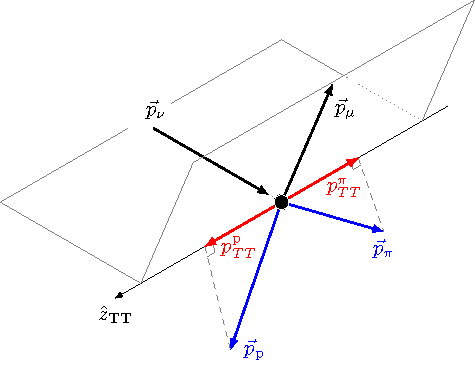
\includegraphics[width=0.35\textwidth]{figures/dptt.pdf}
    \caption{\label{fig:dtki} Schematic illustration of the double TKI variable. Diagram taken from Ref.~\cite{T2K:2021naz}.} 
\end{figure}

In the absence of nuclear effects, $\dptt$ should be zero.
Its distribution width reveals the role of nuclear effects in pion production~\cite{MINERvA:2020anu, T2K:2021naz}.
Analogous variables, $\dptx$ and $\dpty$, have been proposed and studied in MINERvA~\cite{MINERvA:2019ope} for pionless channels.
Additionally, Refs.~\cite{Lu:2015tcr,Hamacher-Baumann:2020ogq} suggest using $\dptt$ to isolate a hydrogen sample.  
More details on hydrogen selections will be given in Sec.~\ref{sec:mc-hydrogen}.

There has been a wealth of TKI-based measurements from multiple neutrino experiments, including T2K~\cite{T2K:2018rnz, T2K:2021naz}, MINERvA~\cite{MINERvA:2018hba, MINERvA:2019ope, MINERvA:2020anu, MINERvA:2021csy}, and MicroBooNE~\cite{MicroBooNE:2022emb, MicroBooNE:2023cmw, MicroBooNE:2023tzj, MicroBooNE:2023wzy, MicroBooNE:2024tmp}.
Because the TKI concept applies equally to electron scattering, experiments such as CLAS~\cite{CLAS:2021neh} have also produced TKI measurements, demonstrating the wide applicability of TKI.

% \begin{savequote}[8cm]
Alles Gescheite ist schon gedacht worden.\\
Man muss nur versuchen, es noch einmal zu denken.

All intelligent thoughts have already been thought;\\
what is necessary is only to try to think them again.
  \qauthor{--- Johann Wolfgang von Goethe \cite{von_goethe_wilhelm_1829}}

Dancing is more important. --- Pauli
\end{savequote}

\chapter{\label{ch:2-neutrinos}The Field of Neutrinos}

\minitoc

\section{The Past}
\section{The Present}
\section{The Plans}


This document introduction won't serve as a complete primer on \LaTeX.  There are plenty of those online, and googling your questions will often get you answers, especially from \url{http://tex.stackexchange.com}.

Instead, let's talk a little about a few of the features and packages lumped into this template situation.  The \verb|savequote| environment at the beginning of chapters can add some wittiness to your thesis.  If you don't like the quotes, just remove that block.

For when it comes time to do corrections, there are two useful commands here.  First, the \verb|mccorrect| command allows you to highlight a short correction \mccorrect{like this one}.  When the thesis is typeset normally, the correction will just appear as part of the text.  However, when you declare \verb|\correctionstrue| in the main \verb|Oxford_Thesis.tex| file, that correction will be highlighted in blue.  That might be useful for submitting a post-viva, corrected copy to your examiners so they can quickly verify you've completed the task.

\begin{mccorrection}
For larger chunks, like this paragraph or indeed entire figures, you can use the \verb|mccorrection| environment.  This environment highlights paragraph-sized and larger blocks with the same blue colour.
\end{mccorrection}

Read through the \verb|Oxford_Thesis.tex| file to see the various options for one- and two-sided printing, including or excluding the separate abstract page, and turning corrections and draft footer on or off, and the separate option to centre your text on the page (for PDF submission) or offset it (for binding).  There is also a separate option for master's degree submissions, which changes identifying information to candidate number and includes a word count.  (Unfortunately, \LaTeX has a hard time doing word counts automatically, so you'll have to enter the count manually if you require this.)

\section{Cardiac Imaging}\label{app:imaging}

Within months of Röntgen's discovery of the X-ray in \mccorrect{1895}\cite{gagliardi_rontgen_1996}, cardiac pathology was being investigated via non-invasive imaging \cite{gagliardi_cardiac_1996}.  Over the intervening years, cardiac imaging modalities and techniques have advanced significantly.  Clinically, cardiac imaging is used for two broad purposes: diagnosis of pathophysiology and guidance of interventional procedures.  These applications impose different requirements on imaging equipment, image acquisition time, computational complexity, spatial and temporal resolution, and tissue discrimination.  The common diagnostic and interventional cardiac imaging techniques in current clinical practice are reviewed below.  An accessible introduction to the physics of medical imaging can be found in Webb's \textit{Introduction to Biomedical Imaging} \cite{webb_introduction_2002}.  A comprehensive overview of the use of imaging in clinical cardiology is presented in Leeson's \textit{Cardiovascular Imaging} \cite{leeson_cardiovascular_2011}.

\subsection{Diagnostic Imaging}
\label{sub:diagnostic}

Beyond the chest X-ray (`plain film'), the key non-invasive imaging modalities in diagnostic cardiology are echocardiography, magnetic resonance imaging, and X-ray computed tomography, which are reviewed below.  Nuclear medicine, including positron emission tomography (PET) and single-photon emission computed tomography (SPECT), are not discussed here, as they do not play a role in the chapters to follow.

\subsubsection{Echocardiography}

\begin{figure}
\centering\includegraphics[width=0.7\textwidth]{figures/sample/Gray498.png} 
\caption[Four-chamber illustration of the human heart.]{Four-chamber illustration of the human heart.  Clockwise from upper-left: right atrium, left atrium, left ventricle, right ventricle.}
\label{fig:fourchamber}\end{figure}

The use of acoustic waves for medical diagnosis, inspired by naval sonar, was initially developed in the 1940s \cite{gagliardi_ultrasonography_1996}.  By 1954, the first clinically useful cardiac ultrasound -- examining motion of the mitral valve in stenosis -- was reported \cite{edler_ultrasonic_1957}.  These early scans were one-dimensional images (`A-mode'), sometimes repeated to generate a time axis (`M-mode').   The sector-scanning probe was developed in the 1970s \cite{bom_ultrasonic_1971,griffith_sector_1974}, leading to the `B-mode' that a modern cardiologist would recognise as an echocardiogram.

% \begin{savequote}[8cm]
\textlatin{Neque porro quisquam est qui dolorem ipsum quia dolor sit amet, consectetur, adipisci velit...}

There is no one who loves pain itself, who seeks after it and wants to have it, simply because it is pain...
  \qauthor{--- Cicero's \textit{de Finibus Bonorum et Malorum}}
\end{savequote}

\chapter{\label{ch:35-nuint}Neutrino interactions} 
\minitoc

\section{nu-quark}
From QFT, write down Fenynman's rule explicitly

\section{nu-nucleon}
However, due to confinement and the relatively low energy, nu usually is interacting with the nucleon as a whole.
require form factors to paramterize the interaction with a nucleon.

\section{nu-nucleus}
Nuclear effect. 
The simplest case is for the relatively high energy nu, for wthich Impulse Approximation (IA) can be used.
Nu sees the nucleon as independent from other nucleons.
The interaction approaches the nu-nucleon interaction.

When the energy drops, IA is no longer valid and see the nucleus as a whole.
RPA correction is needed, beyond the scope of this thesis, will not ellaborate but interest reader can refer to REFXXX for more details.

  \subsection{Initial state}
  In addition to the different modes that the neutrino ineteract with the nucleus, the presence of the nuclear medium also affects the interaction.
  The nuclear effects manifest in two ways.
  Firstly, the nucleon in the interaction is in a bound state, i.e. it cannot have arbitrary energy and momentum like a free nucleon.
  Instead, the energy distribution of the nucleon is parameterised by the so-called Spectral Function (SF).
  The simplest form of SF is the Fermi Gas model, which treats the nucleons as freely moving Fermi gas.
  Hence, the nucleon momentum is filled up to the Fermi momentum, which is given as:
  <CHECK>
  \begin{equation}
      k_F = (3\pi^2 \rho/2)^{1/3},
  \end{equation}
  where $\rho$ is the nuclear density.
  <How is the fermi momentum determined?>
  This model oversimplifies the nuclear structure.
  A more realistic model is the local Fermi gas (LFG) model, which accounts for the varying nuclear density, leading to an SF of the form:
  (CHECK)
  \begin{equation}
      S(k, E) = \int \rho(\vec{r}) \delta(E - \sqrt{k^2 + m^2}) d^3r,
  \end{equation}
  where $m$ is the nucleon mass.

  Further improvement, such as the short-range correlation between nucleons that increases the high momentum fraction.
  There are also effective SFs. Fit to data?

  \subsection{FSI}
  \label{sec:nuint-fsi}
  The second nuclear effect is the Final State Interaction (FSI).
  Regardless of how the neutrino interacts with the nucleon, the interaction products are still inside the nucleus.
  They have to propagate through the nuclear medium to be detectable.
  The interactions with the nuclear medium are classified as FSI.
  They are more pronounced for hadrons than leptons, as the former are more likely to interact with the nuclear medium.
  There are several types of FSI, such as the elastic scattering, charge exchange, and absorption.
  \begin{enumerate}
      \item 
  CEX involves changing the charge of the participating particles; for example,
  \begin{equation}
      \pip + \n \rightarrow \piz + \p,
  \end{equation}
  or vice versa. This rescattering type is crucial for event topologies requiring the presence of a pion;  depending on the signal pion charge, CEX could migrate events between signal and background. 

  \item 
  INEL is the case where the nucleus is left in an excited state after the rescattering. This category only contains the situation where a single additional nucleon is emitted/knocked-out after rescattering. Since it does not affect the number of pions produced, it will not convert an event from a pionless topology to a pion-production topology. The effects on nucleons are two-fold. Firstly, it can alter the number of signal events within each event topology. If the inelastic rescattering leads to two low-momentum protons below the detection threshold as opposed to a high-momentum proton, this signal event will be discarded as no protons are observed. Secondly, INEL invariably changes the kinematics of the rescattering particle. Be it the leading proton or the leading pion, based on which the TKI observables are calculated, the TKI distribution shape will be affected. Hence, while $\ninel$ would affect all four data sets, $\piinel$ would only affect \ttkpip and \minpiz. 

  \item 
  ABS refers to the case where the particle undergoes an interaction so that it does not emerge as a final particle. For example, $\pi^+$ can interact with two or more nucleons, initially forming a baryon resonance that subsequently interacts with other nucleons, emitting multiple nucleons rather than pions. Hence, the $\pi^+$ would not emerge from the nucleus anymore.

  \item 
  PIPD happens for energetic particles where an extra pion emerges as a result of the rescattering, such as
  \begin{equation}
      \p + \p \rightarrow \p + \n + \pip.
  \end{equation}
  Such an interaction significantly alters the event topology. 

  \end{enumerate}


\section{\label{sec:1-intro}Introduction}

Neutrinos play a central role in advancing our understanding of physics and addressing fundamental inquiries in contemporary science. The Hyper-Kamiokande experiment~\cite{Hyper-Kamiokande:2018ofw} aims to conduct precise measurements of charge parity violation within the neutrino sector, a phenomenon believed to be closely linked to the observed matter-antimatter asymmetry in the universe. Similarly, the Deep Underground Neutrino Experiment (DUNE)~\cite{DUNE:2016hlj,DUNE:2015lol,DUNE:2016evb,DUNE:2016rla,DUNE:2021tad}  promises the same, in addition to elucidating the neutrino mass ordering. Whether seeking to ascertain Standard Model parameters or probing for exotic phenomena, significant enhancements in both theoretical frameworks and computational simulations of neutrino-nucleus interactions are imperative. As neutrinos interact mainly with nucleons inside the nucleus, the interaction is subject to nuclear effects, namely the nucleon initial state and final-state interactions (FSIs). These effects are difficult to calculate and can alter the final event topology by changing the number of final state pions with respect to the interactions on free nucleons. Notably, the neutrino flux at DUNE yields a comparable proportion of events with and without pions in the final state, highlighting the pressing need for a generator capable of accurately describing both event topologies.

The large data samples and superb imaging capabilities of modern neutrino experiments offer us a detailed new look at neutrino interaction physics.
Recently, the GENIE~\cite{Andreopoulos:2009rq, GENIE:2021npt} Collaboration has made substantial progress towards a global tuning using neutrino, charged lepton and hadron scattering data, in an attempt to integrate new experimental constraints with state-of-the-art theories and construct robust and comprehensive simulations of neutrino interactions with matter. 
Cross-experiment and cross-topology analyses are challenging tasks as each measurement features its unique selection criteria and various other  aspects, such as the neutrino flux. \genie has built an advanced tuning framework that enables the validation and tuning of comprehensive interaction models using an extensive curated database of measurements of neutrino, charged lepton and hadron scattering off nucleus and nuclei. So far, the non-resonant backgrounds~\cite{GENIE:2021zuu}, hadronization~\cite{GENIE:2021wox} and the quasielastic (QE) and 2-particle-2-hole (2p2h)  components~\cite{GENIE:2022qrc} of the neutrino-nucleus interaction have been tuned with $\nu_\mu$ and $\bar{\nu}_\mu$ charged-current (CC) pionless (0$\pi$) data from MiniBooNE, T2K and MINERvA. A partial tune was performed for each experiment, highlighting the neutrino energy dependence on the QE and 2p2h tuned cross sections. Even though post-tune predictions enhanced the data description for each experiment, the added degrees of freedom were not sufficient to fully describe all CC0$\pi$ data and exhibited tensions with some proton observables~\cite{GENIE:2022qrc}. More exclusive measurements result in additional model constraints. In addition, observables that are sensitive to targeted aspects of the complex dynamics of neutrino interactions are invaluable for model tuning. The transverse kinematic imbalance (TKI)~\cite{Lu:2015hea, Lu:2015tcr}, a final-state correlation between the CC lepton and the handronic system, is a good example since it is sensitive to the initial-state nuclear environment and hadronic FSI. Our next step is to incorporate TKI data from experiments where various exclusive topologies at different energies are considered. This marks the first combined tuning on TKI data with and without pions in the final states and serves as the starting point of a more comprehensive tuning effort in the energy region most relevant for future accelerator-based neutrino experiments.  


\section{TKI}
\label{sec:nuint-tki}

\begin{figure}[!htb] 	
    \centering 		
    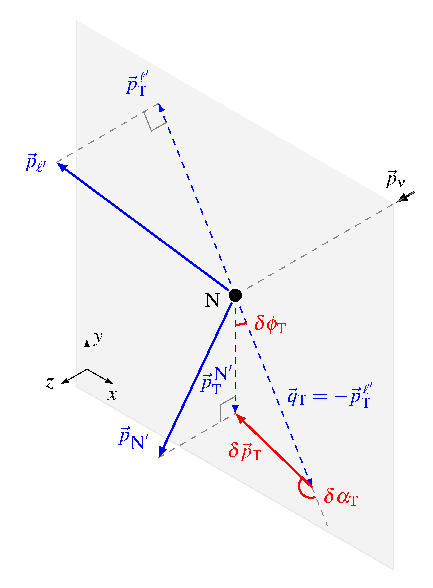
\includegraphics[width=0.35\textwidth]{figures/stki.eps}
    \caption{\label{fig:stki} Schematic illustration of the TKI variables. Diagram taken from Ref.~\cite{Lu:2015tcr}.} 
\end{figure}

The TKI variables are shown in Fig.~\ref{fig:stki}. They are cleverly constructed such that they are most sensitive to IS and FSI. 
In the simplest case, there are only two final particles after the neutrino-nucleon interaction, a muon and a proton. 
If the initial momentum of the struck nucleon has no component transverse to the neutrino's incoming direction, the products, i.e. the muon and the proton, should not have a net transverse component either, unless the struck nucleon has a non-zero initial transverse component or the final particles have undergone FSI.
Suppose there is no FSI, the net transverse component, $\dpt$, corresponds exactly to the magnitude of the transverse component of the struck nucleon, and the angle, $\dat$, represents the direction of the initial nucleon motion projected on the transverse plane. 
Assuming the nucleons are moving isotropically, the $\dat$ distribution should be flat. 
All current nuclear models do not have a preferential direction for initial nuclear motion, so it is only natural to assume the nucleons move in random directions. 
Thus, the deviation from flatness for $\dat$ can only be due to FSI, thereby making it an excellent probe for FSI. 
As for $\dpt$, it reflects the magnitude of the initial nucleon momentum transverse to the neutrino direction compounded by FSI. 
Furthermore, if the nucleus is assumed to be at rest and no other particles are knocked out other than the muon and the proton, the initial nucleon momentum, $\pn$, can also be derived following the steps outlined in \cite{pnpaper}. 
 

\section{TKI measurements}\label{sec:tki}


TKI is a methodology based on the conservation of momentum in neutrino interactions. In essence, it involves quantifying the imbalance between the observed transverse momentum of the final-state particles and the expected transverse momentum from neutrino interactions with free nucleons~\cite{Lu:2015hea, Lu:2015tcr}. This ``kinematic mismatch'' together with its longitudinal and three-dimensional variations~\cite{Furmanski:2016wqo, Lu:2019nmf}, and the derived asymmetry~\cite{Cai:2019jzk}, has been a crucial set of observables, establishing a pathway to extract valuable information about the participating particles and the underlying nuclear processes. Recent experimental results from neutrino experiments such as  T2K~\cite{T2K:2018rnz, T2K:2021naz}, MINERvA~\cite{MINERvA:2018hba, MINERvA:2019ope, MINERvA:2020anu, MINERvA:2021csy}, and MicroBooNE~\cite{MicroBooNE:2022emb, MicroBooNE:2023cmw, MicroBooNE:2023tzj, MicroBooNE:2023wzy, MicroBooNE:2024tmp}, as well as electron scattering experiments such as  CLAS~\cite{CLAS:2021neh}, highlight the efficacy of TKI. 

\begin{figure}[!htb] 	
    \centering 		
    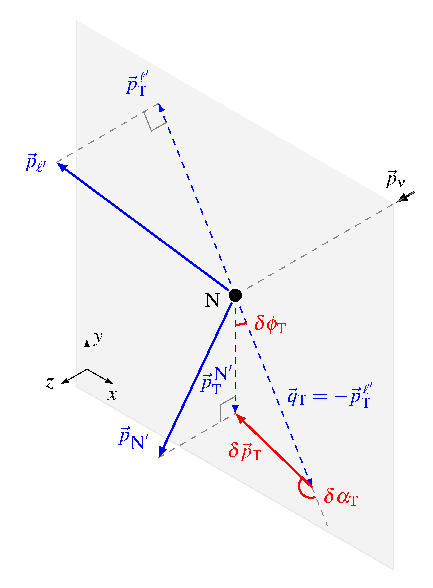
\includegraphics[width=0.35\textwidth]{figures/stki.eps}
    \caption{\label{fig:stki} Schematic illustration of the TKI variables. Diagram taken from Ref.~\cite{Lu:2015tcr}.} 
\end{figure}

In neutrino scattering off a free nucleon, the sum of the transverse components of the final products is expected to be zero, visualized through a back-to-back configuration between the final-state lepton and hadronic system in the  plane transverse to the neutrino direction. Hence, in a neutrino interaction with a nucleus, the transverse momentum imbalance, $\dpt$~\cite{Lu:2015tcr}, results from intranuclear dynamics, including Fermi motion and FSIs  as shown in Fig.~\ref{fig:stki}. The deviation from being back-to-back is quantified by the  coplanarity angle $\dphit$~\cite{Lu:2015tcr}, while the transverse boosting angle, $\dat$~\cite{Lu:2015tcr}, represents the direction of $\dpt$ within the transverse plane. Furthermore, analyzing the energy and longitudinal momentum budget~\cite{Furmanski:2016wqo, Lu:2019nmf} enables the conversion of $\dpt$ to the emulated (initial) nucleon momentum, $\pn$,  providing further insight into the Fermi motion; this conversion amounts to a correction on the order of $\mathcal{O}(20\%)$~\cite{Yang:2023dxk}. 
With one-body currents in the absence of FSIs, $\dat$ remains uniform (except for second-order effects, such as variations in the center-of-mass energy), given the isotropic nature of the initial nucleon motion. However, as the final products propagate through the nuclear medium, they experience FSIs, thereby disturbing the isotropy and the Fermi motion peak of the $\dat$ and $\pn$ ($\dpt$) distributions, respectively. Hence, $\dpt$ and $\pn$ elucidate the Fermi motion details, while $\dat$  characterizes the FSI strength---crucial for understanding medium effects in neutrino interactions. A notable advantage of these observables is their minimal dependence on neutrino energy~\cite{Lu:2015tcr}. Moreover, the double TKI variable, $\dptt$~\cite{Lu:2015hea}, is the projection of $\vecdpt$ along the axis perpendicular to the lepton scattering plane (hence ``double''). In addition to its use for extracting neutrino-hydrogen interactions~\cite{Lu:2015hea, Hamacher-Baumann:2020ogq}, it has also been applied to study nuclear effects in neutrino pion productions~\cite{MINERvA:2020anu, T2K:2021naz}. Its equivalent in pionless production, $\dptx$, has been proposed and studied together with its orthogonal companion, $\dpty$, in MINERvA~\cite{MINERvA:2019ope}. 
\begin{savequote}[8cm]
\begin{CJK*}{UTF8}{min}
おれは海賊王になる男だ!!!
\end{CJK*}

I'll be the one to measure $\dcp$.
  \qauthor{--- Monkey D. Luffy}
\end{savequote}

\chapter{\label{ch:t2k}The T2K Experiment} 

\minitoc
The T2K experiment is a long-baseline neutrino experiment with the aim of measuring CP violation in the lepton sector through neutrino oscillation measurements.  
This chapter begins by describing the experimental setup and then provides a concise overview of the software, thereby laying the groundwork for the subsequent analyses.

\section{Hardware}
As a long-baseline experiment, T2K encompasses a near detector (ND280) and a far detector (Super-Kamiokande, often referred to as Super-K).  
Both detectors must discriminate between \(\numu\) and \(\nue\) to measure neutrino oscillations.  
Naturally, detecting neutrinos directly is impossible.  
Instead, each detector must be able to identify the different particles produced when neutrinos interact with its active material.  
Most commonly, such neutrino–nucleus interactions generate the corresponding leptons (i.e., electrons or muons) and various hadrons, including protons, neutrons, and light mesons such as pions.

The far detector, SK, is a large water Cherenkov detector.  
It detects particles by collecting the Cherenkov light emitted when they travel faster than the speed of light in water.  
Hadrons resulting from neutrino interactions typically lack sufficient energy to emit Cherenkov radiation, whereas leptons often exceed this threshold.  
Consequently, SK primarily observes electrons and muons, whose Cherenkov radiation forms ring-like patterns transverse to their direction of flight.  
Because the electron is lighter than the muon, its path is more prone to scattering, causing the electron’s Cherenkov ring to appear more diffuse than the muon’s, as illustrated in Fig.~\ref{fig:sk-e-mu}.

\begin{figure}
    \centering
    \begin{subfigure}[b]{\dbfigwid\textwidth}
        \centering
        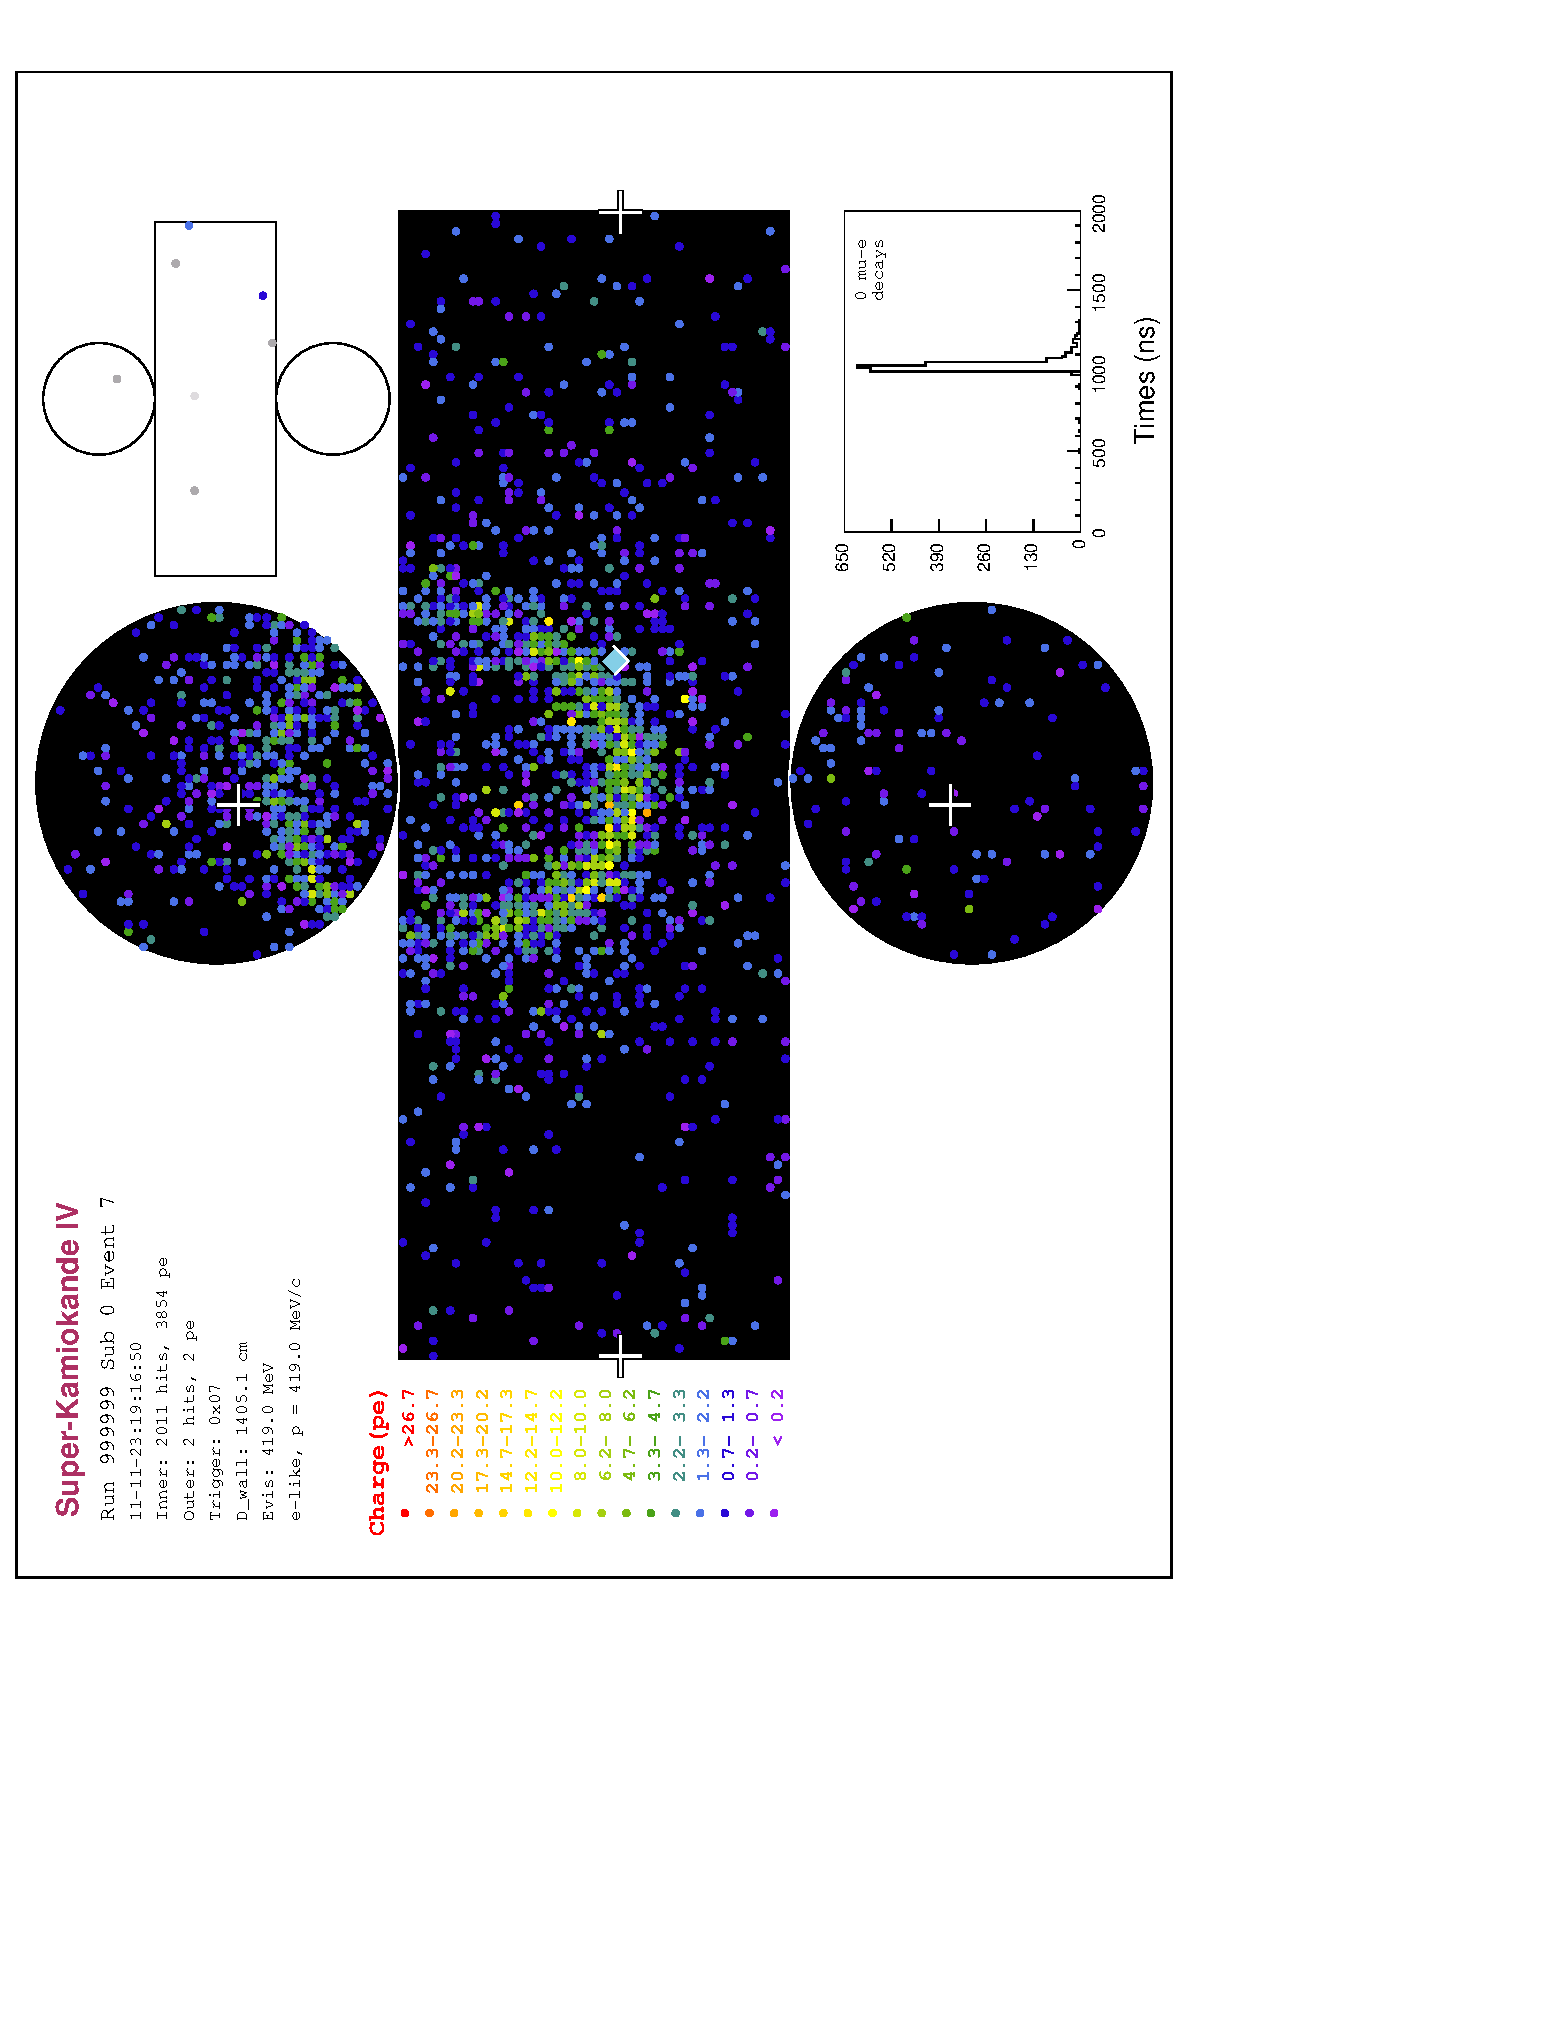
\includegraphics[width=\textwidth]{figures/t2k/sk-nue.eps}
        \caption{\(\nu_e\)}
        \label{subfig:sk-nue}
    \end{subfigure}
    \begin{subfigure}[b]{\dbfigwid\textwidth}
        \centering
        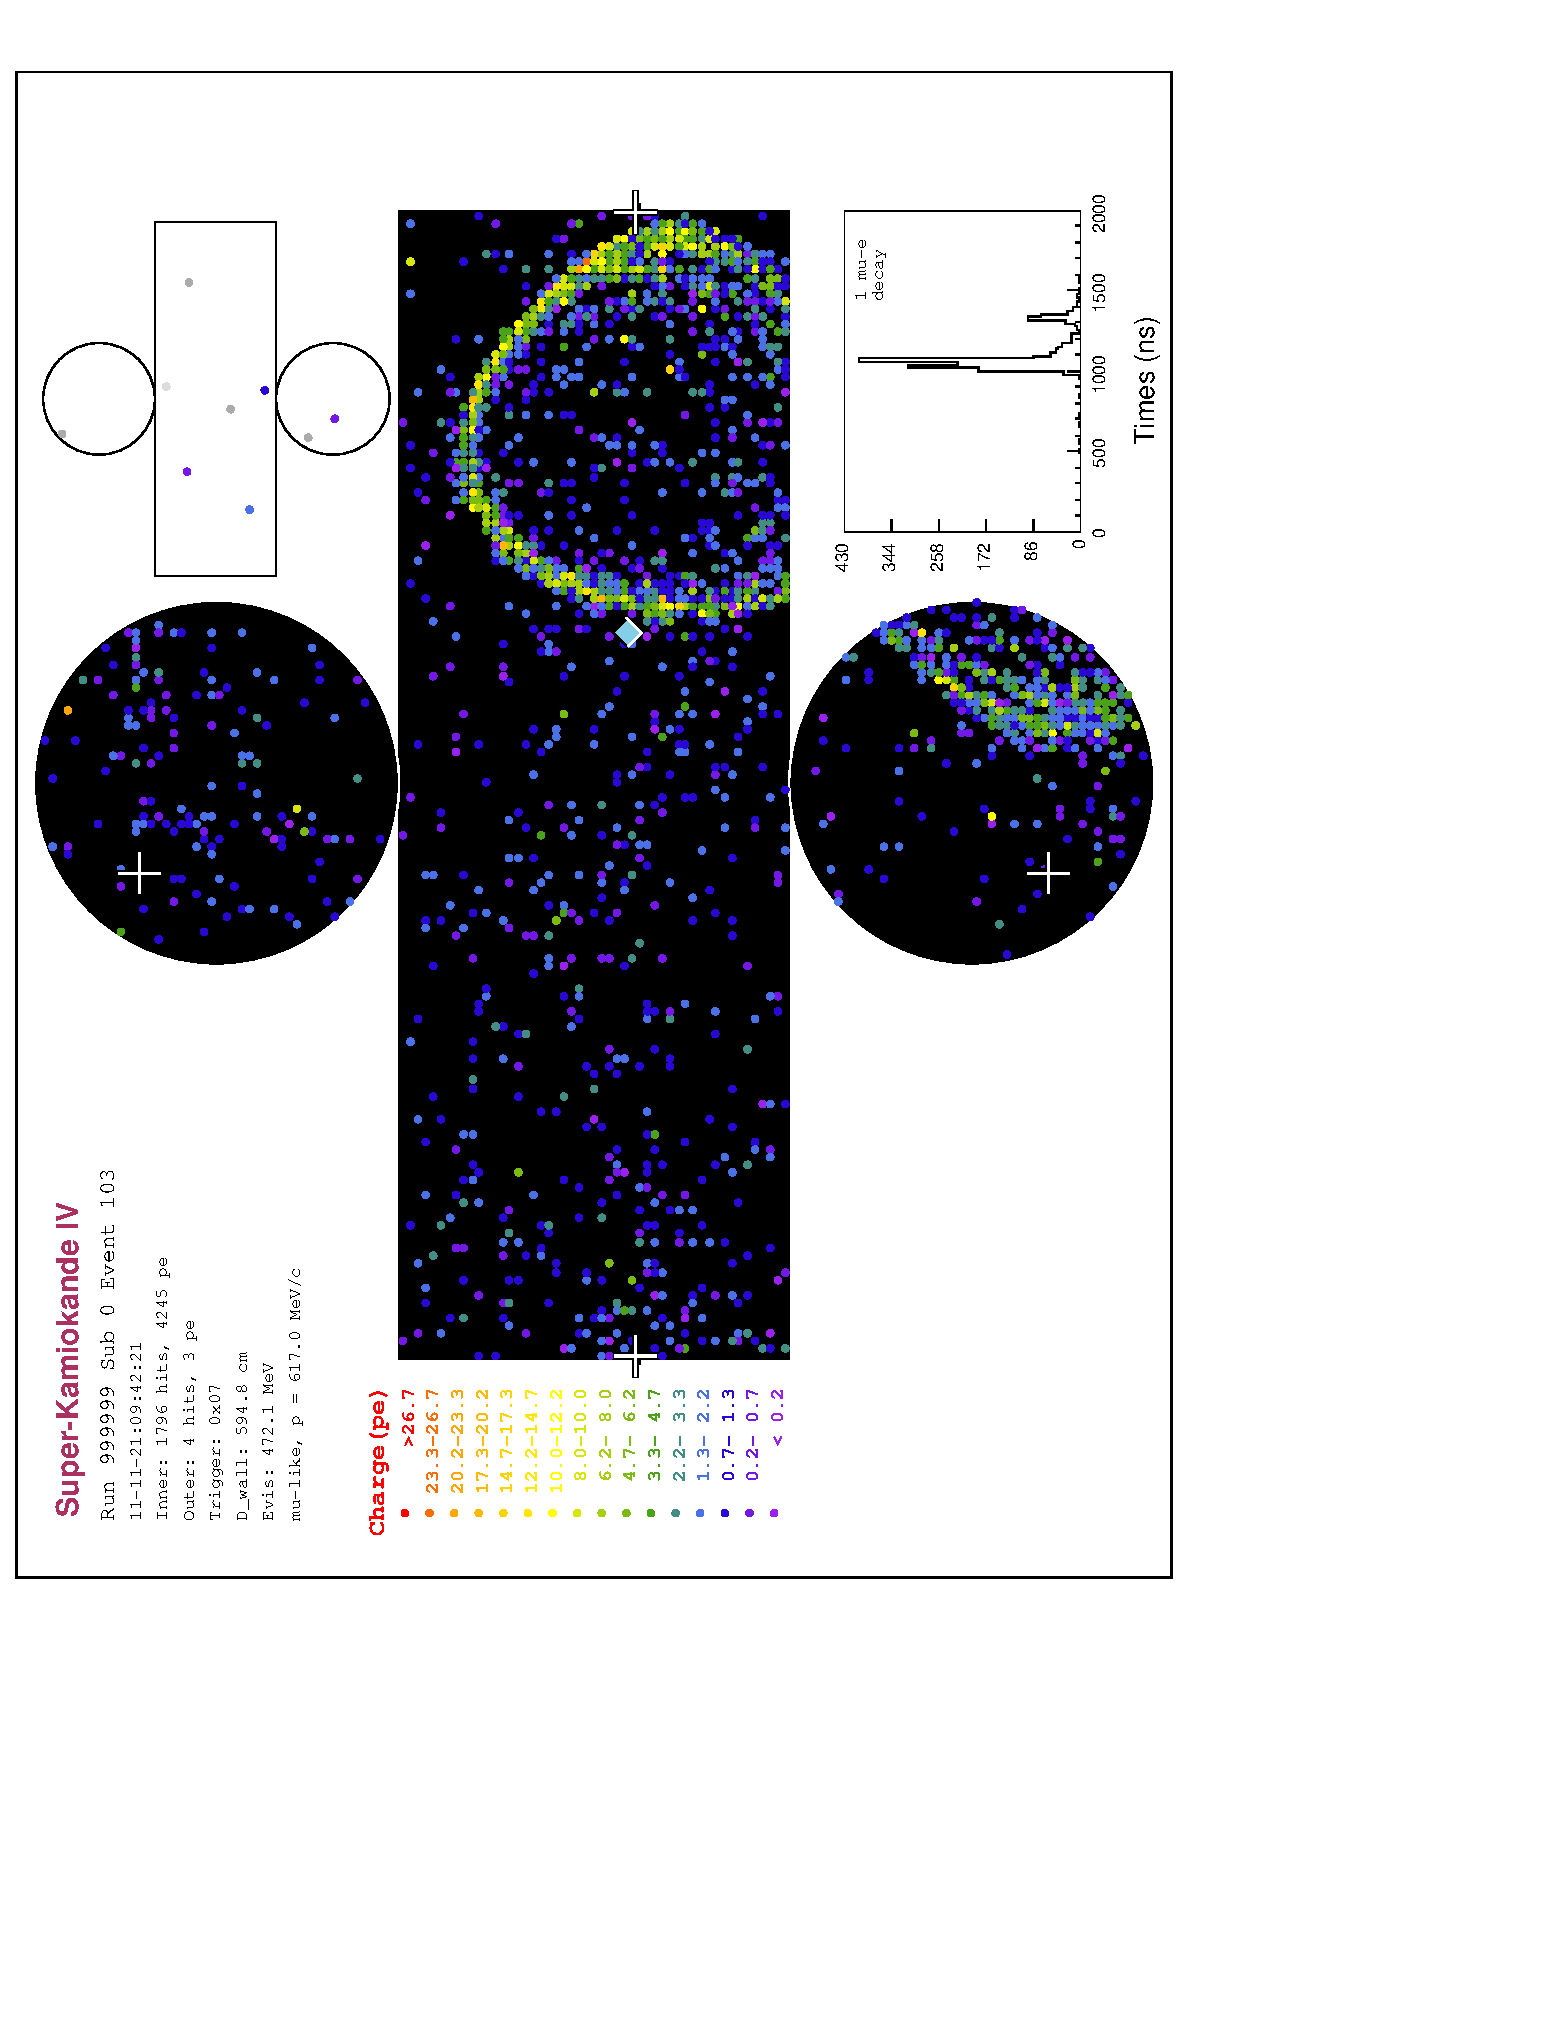
\includegraphics[width=\textwidth]{figures/t2k/sk-numu.eps}
        \caption{\(\nu_\mu\)}
        \label{subfig:sk-numu}
    \end{subfigure}
    \caption{SK event displays.}
    \label{fig:sk-e-mu}
\end{figure}

In contrast, the near detector, ND280, consists of multiple specialized subdetectors designed to measure hadrons.  
The classic ND280 configuration is shown in Fig.~\ref{subfig:nd280-classic}.  
Its central detector assembly contains a \(\piz\)-detector (P0D), three vertical Time Projection Chambers (TPCs), and two Fine Grained Detectors (FGDs) positioned between the TPCs.  
Surrounding these devices are various electromagnetic calorimeters (ECALs)—the P0D ECAL, the Barrel ECAL, the Upstream ECAL, and the Downstream ECAL—all enclosed by the UA1 magnet comprising a solenoid coil and a yoke.

\begin{figure}
    \centering
    \begin{subfigure}[b]{\dbfigwid\textwidth}
        \centering
        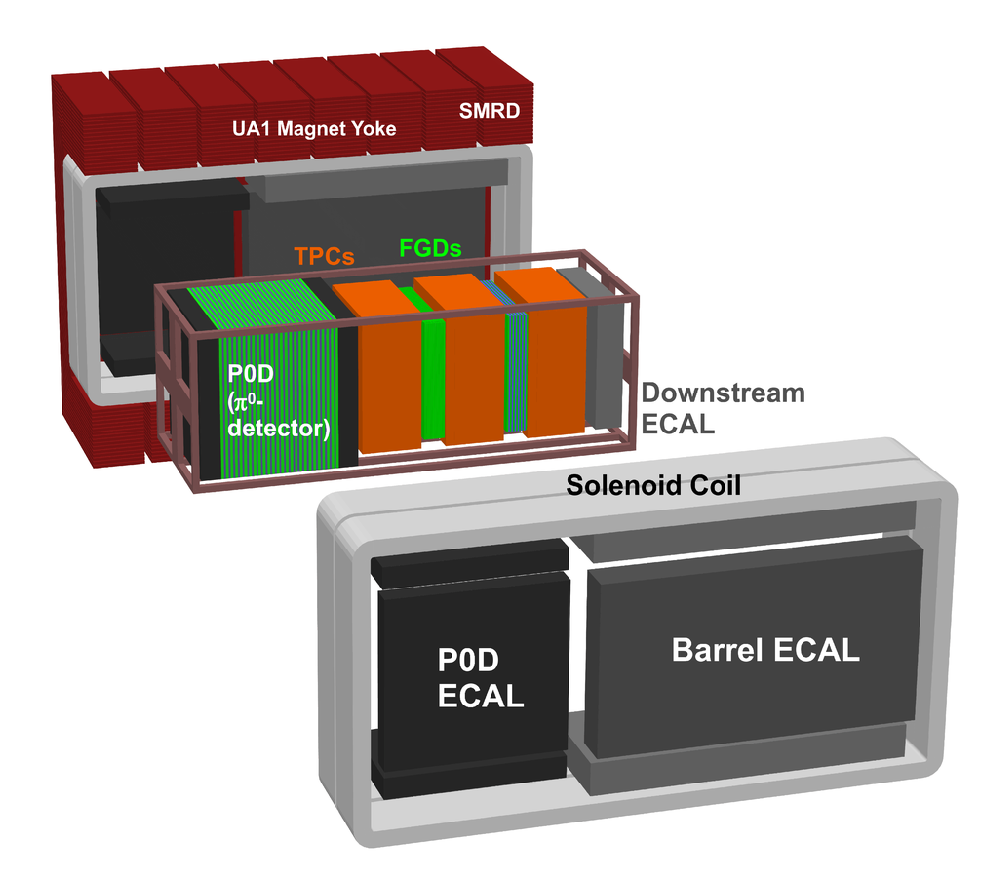
\includegraphics[width=\textwidth]{figures/t2k/ND280-classic.eps}
        \caption{Classic}
        \label{subfig:nd280-classic}
    \end{subfigure}
    \begin{subfigure}[b]{\dbfigwid\textwidth}
        \centering
        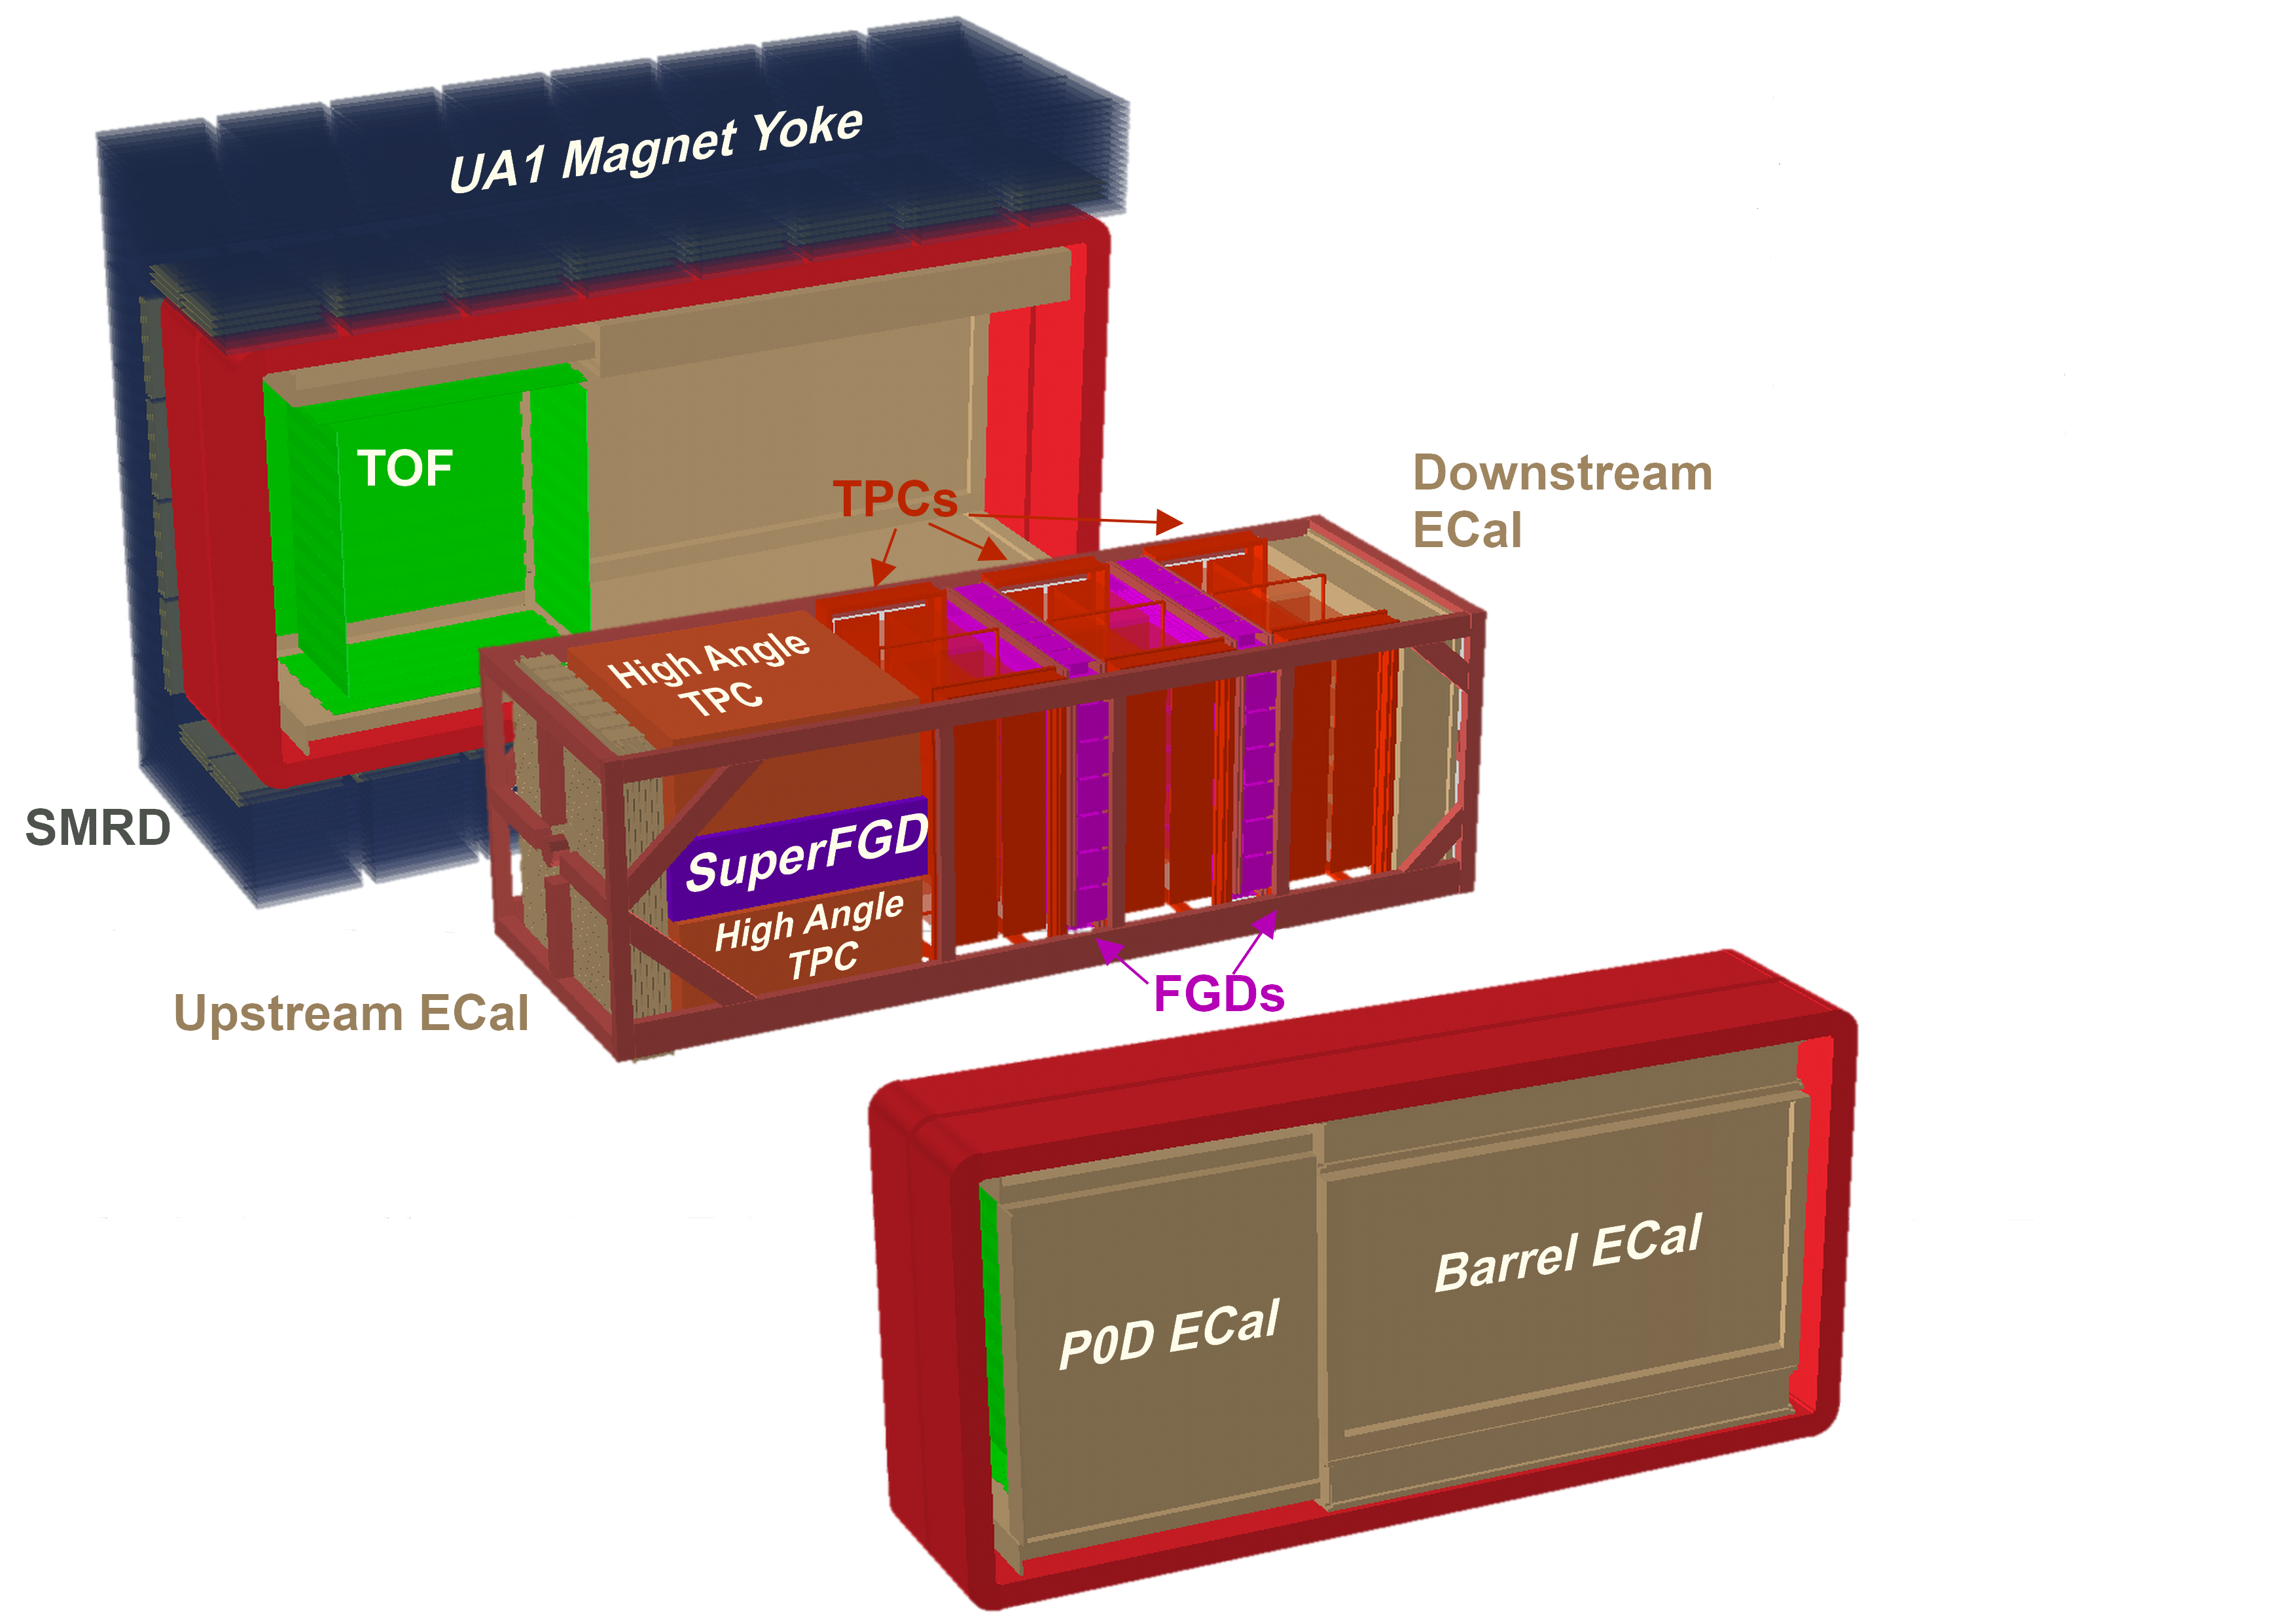
\includegraphics[width=\textwidth]{figures/t2k/ND280-up.png}
        \caption{Upgrade}
        \label{subfig:nd280-up}
    \end{subfigure}
    \caption{ND280 detector diagram.}
    \label{fig:nd280-diagram}
\end{figure}

The neutrino beam passes through the P0D, TPCs, and FGDs.  
Each FGD consists of scintillator bars with a cross section of \(1.0~\mathrm{cm} \times 1.0~\mathrm{cm}\).  
Every layer of bars is oriented orthogonally to the layer above it.  
As a particle traverses these layers, it excites photons in the scintillator; these photons are collected by wavelength-shifting fibers embedded in each bar and ultimately read out by end electronics.  
Hence, the bar recording the signal determines the track position transverse to the neutrino beam, while the layer index specifies the longitudinal position of the energy deposition.

Originally, FGDs served as the active target for neutrino interactions.  
However, their bar geometry offers limited acceptance for particles traveling at large angles to the beam direction—i.e., along the bar’s long axis—because such particles intersect only a few bars, making them difficult to reconstruct.  
This mismatch in phase space between the near and far detectors increases uncertainties in oscillation analyses.  
Moreover, having sparse signals along the particle trajectory degrades reconstruction resolution.  
These limitations motivated the ND280 upgrade.

In the upgraded ND280, the \(\piz\)-detector is replaced by several new subsystems (Fig.~\ref{subfig:nd280-up}): the Time-of-Flight detector (TOF), two High-Angle TPCs (HATs), and the Super Fine Grained Detector (SFGD).  
The TOF comprises six layers of scintillator bars with sub-nanosecond timing resolution, which help veto crossing particles and enhance sample purity.  
The HATs incorporate a redesigned field cage and new Micromegas detectors, expanding the tracking volume and improving resolution relative to the original vertical TPCs.  
Serving as the new active target, the SFGD consists of about two million \(1\,\mathrm{cm}^3\) scintillator cubes.  
Its finer segmentation markedly increases acceptance for high-angle tracks, better aligning with the near-isotropic acceptance at the far detector.  
Additionally, the improved tracking, enabled by enhanced energy deposition measurements, lowers detection thresholds and sharpens resolution, facilitating new reconstruction strategies (e.g., trackless pion reconstruction) and innovative variables (e.g., center-of-mass variables), which will be introduced in the next chapter.  
Construction for the upgrade was completed in April 2024, and data taking with the upgraded ND280 commenced in June 2024.

\section{Software}
\label{sec:t2k-sw}
This thesis focuses primarily on improving reconstruction performance; thus, the following overview of the software used for ND280’s upgraded system aims to clarify and contextualize the methodologies employed in later chapters.

Each scintillator cube in the SFGD contains an optical fiber, forming an electronic signal channel.  
As a charged particle traverses these cubes, scintillation photons are collected by readout boards located on three orthogonal faces of the SFGD.  
After calibration, these signals are digitized and assembled into three-dimensional “Hits,” each corresponding to a specific cube position and including a measure of deposited charge.  
The reconstruction software then sorts these Hits into either clusters or tracks using clustering and track-fitting algorithms.  
Clusters consist of fewer than three Hits, whereas tracks typically contain many more.  
Additionally, due to imperfect optical isolation between cubes, light may leak into neighboring cubes not actually traversed by the particle.  
To account for this, the reconstruction merges nearby Hits into “Nodes,” which more accurately capture the particle’s trajectory.  
Energy deposition at each Node is then estimated from the associated Hits and refined according to the expected continuous energy loss along the path.  
Finally, a Boosted Decision Tree (BDT), trained on Particle Gun simulations, uses these smoothed energy values and other measured parameters for particle identification and momentum estimation.  
\begin{savequote}[8cm]
\begin{CJK*}{UTF8}{gbsn}
  银鞍照白马,飒沓如流星。
\end{CJK*}

With great techniques come great measurements.
  \qauthor{--- Bai Li \textit{Xia Ke Xing}}

\end{savequote}

\chapter{\label{ch:techniques}New Techniques in Selection Development} 
\minitoc

The upgraded detector has enhanced measuring capabilities, which is especially important for hadrons,
As hadrons tend to have much shorter tracks and are conventionally harder to reconstruct in scintillator detectors compared to muons, the previously explored hadronic kinematic phase space has been relatively restricted, and the reconstructed hadronic variables have relatively large uncertainties.
Since more exclusive event topologies, such as $\numuccopiop$, allow the measurement of high-level variables like the Transverse Kinematic Imbalance (TKI) variables, which provide invaluable insights on neutrino-nucleus interactions, it is highly desirable to reconstruct hadrons, measure their kinematic properties as precisely as possible, and explore their phase space as extensively as possible.

Two of the most common product hadrons from neutrino-nucleus interactions are protons and pions. 
The default particle identification and momentum reconstruction have been developed by colleagues at T2K using the Boosted Decision Tree (BDT) algorithm, which is a machine learning algorithm that takes the energy deposit as the input and outputs the particle identity and momentum. 
The BDT algorithm has good performance, but it is still lacking in some aspects.
For instance, as it uses only single-track information, it cannot effectively distinguish between pions and muons. 
It can reconstruct proton momentum with an excellent resolution of about $3.5\%$, but it is insufficient for TKI analysis, which is highly sensitive to hadron kinematics. 

To address these gaps, I have developed and implemented new techniques for both hadrons, exploiting the precise position and $\dedx$ measurements and timing resolution.
For pions, I have invented the pion trackless reconstruction, a novel technique to reconstruct pions without requiring the presence of a reconstructed track, thereby lowering the detection threshold and significantly increasing reconstruction efficiency for low-momentum pions. 
As for protons, I have adapted the Elastically Scattered and Contained (ESC) protons technique~\cite{Lu:2016mjf} to SFGD, showing significant improvement in proton momentum reconstruction resolution,  
These new techniques are applied in the development of two signal sample selections, namely the $\numucczpiop$-ESC selection and the $\numuccopi$-TL selection, where the ``TL'' refers to the use of the trackless reconstruction technique.
Additionally, to prepare for the data-MC comparisons and future cross-section analysis, I have also developed a stopping pion control sample selection.

\section{$\numucczpiop$-ESC}
\label{sec:sel-esc}
     % The $\numucczpiop$-ESC adds an additional ESC selection step to the $\numucczpiop$ selection developed by a T2K colleague.
     % The details of the ESC step are elaborated below.
   %------------------- ESC ----------------%
    \subsection{Working Principles of the ESC technique}
    \label{sec:sel-esc-wp}
     The subsection elaborates on the underlying principles of the ESC selection technique.
     Protons coming to rest deposit a large amount of energy within a short distance just before stopping.
     Hence, for these protons, if the energy deposited per distance, $\dedx$, is plotted along the particle trajectory, a peak, the so-called Bragg Peak, appears near the track end.
     This feature can be exploited to select protons that come to rest without undergoing secondary interactions, which are thus called "elastically scattered" protons by the original developer of the technique~\cite{Lu:2016mjf}.
     To identify the Bragg peak, the entire proton track must be contained within the scintillation detector such that the $\dedx$ can be measured at the end of the track.
     Thus, this technique is called the elastically scattered and contained technique.
     These ESC protons are of particular interest because their range is strongly correlated with their momentum, which could be exploited by the machine learning algorithm.
     Hence, even though all proton momenta are reconstructed by the BDT algorithm, the ESC protons tend to better momentum reconstruction resolution.

     In the SFGD, having the Bragg peak implies large $\dedx$ for the last few nodes of the proton track.
     For illustration, the fractional difference between the reconstructed and true proton momentum is plotted against the energy deposited at the third last node of the proton track in Fig.~\ref{fig:dedx-pprres-eg} with column normalization.
     More specifically, all bins with the same $x$ value are considered to be in the same column, and the bin height is normalized by the largest bin height in the column.
     Thus, the maximum value in each column is $1$, thereby visualising the comparison between columns.
     For instance, in Fig.~\ref{fig:dedx-pprres-eg}, the red bins (the bin with the largest value) concentrate around $y=0$, i.e. small differences between reconstructed and true proton momentum, for columns having $\dedx$ above $1000$ arbitrary units\footnote{ 
     The energy deposit output from the SFGD reconstruction does not have a physical unit, but its magnitude is an algorithmic estimate of the energy deposited by the particle at each node.}, while for columns with $\dedx$ below $1000$, the red bins deviate from $y=0$ with larger fluctuations.
     Thus, selecting protons with large $\dedx$ for the last few nodes of the proton track can produce a sample with good proton momentum reconstruction resolution.
     This is the underlying principle of the ESC technique.
    \begin{figure}[htb]
        \centering
     %    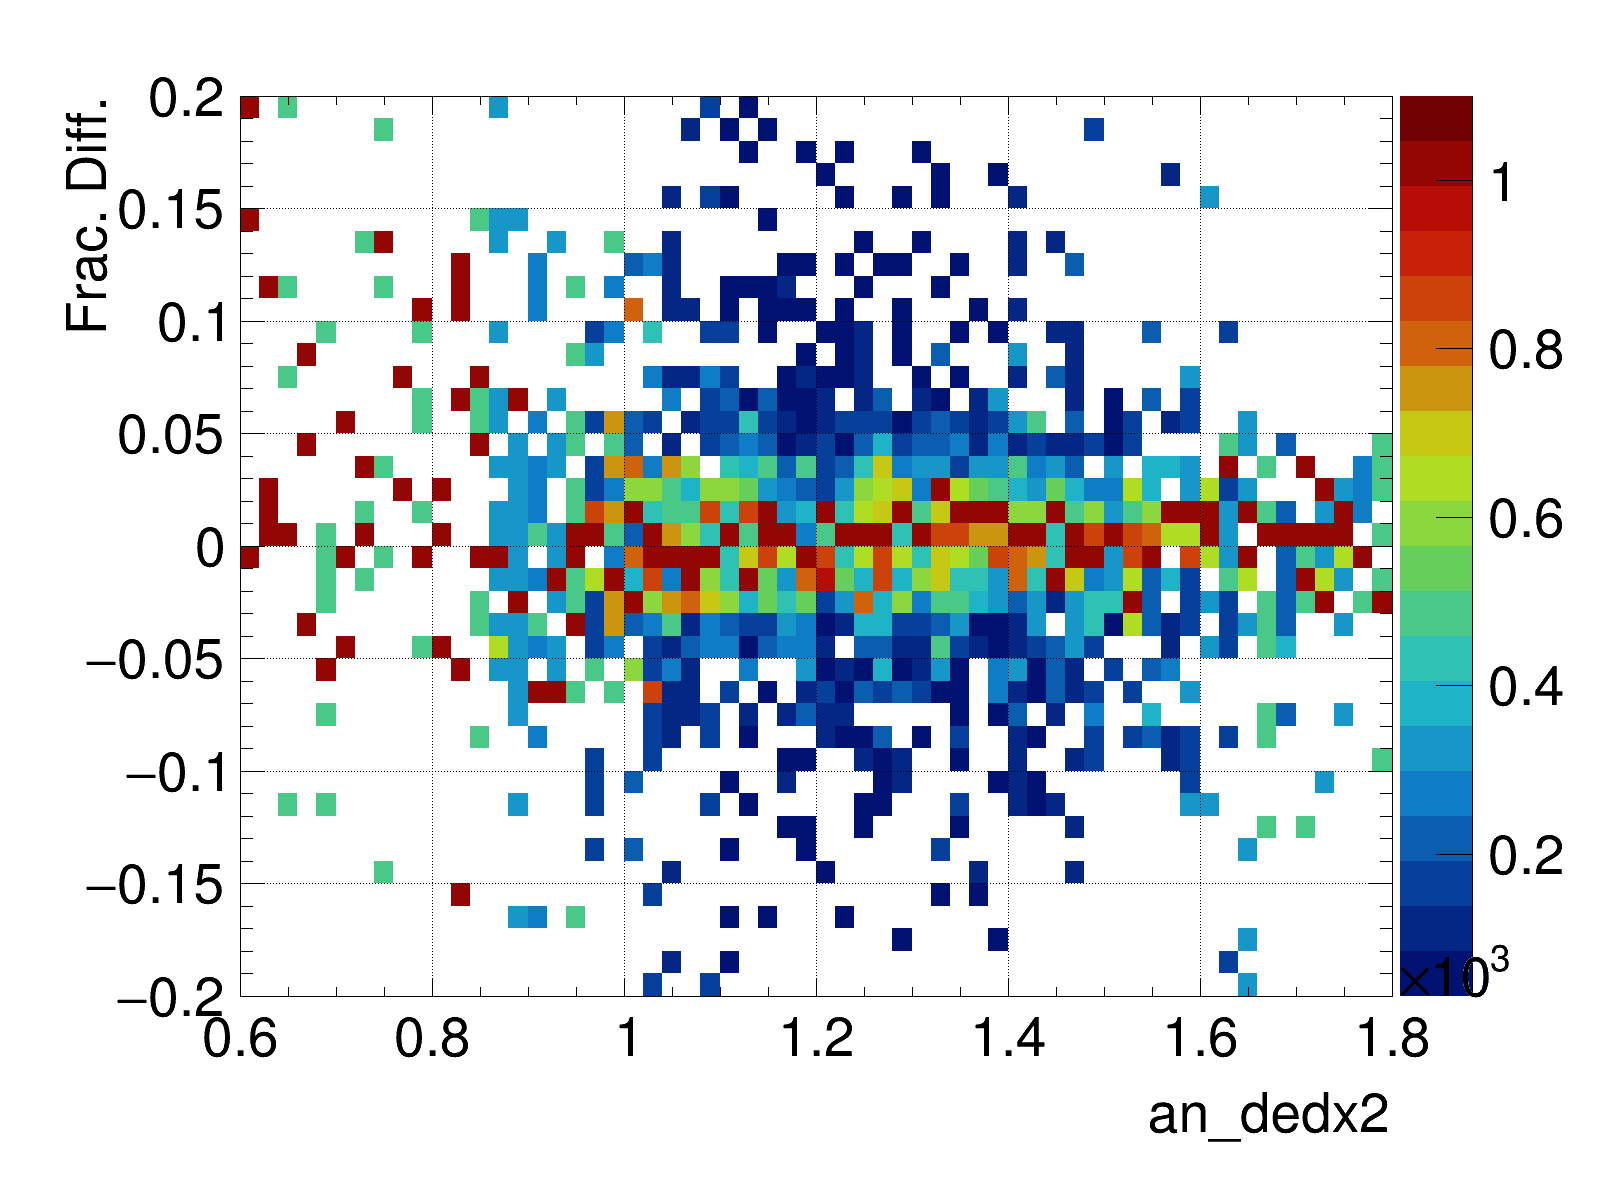
\includegraphics[width=\sgfidwid\linewidth]{figures/sel/an_dedx2_colnor_vs_p_pr_res_hist2d_al12_zoom.png}
        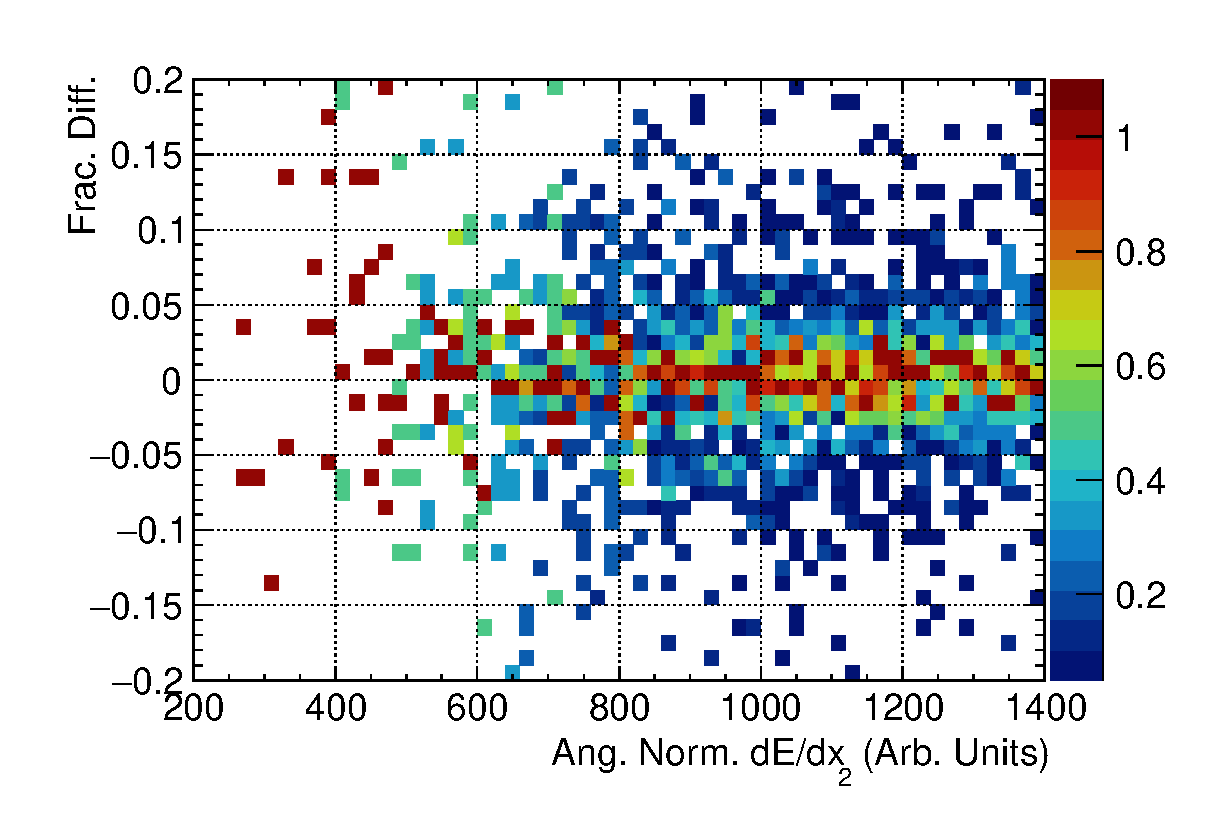
\includegraphics[width=\sgfidwid\linewidth]{figures/sel/fig51.eps}
        \caption{Proton momentum fractional difference against angular normalized $\dedx$ (detailed explanation of this quantity is given in the next subsection) at the second last node. Considerable fluctuations occur when the }
        \label{fig:dedx-pprres-eg}
    \end{figure}
    
   \subsection{Implementation}
   \label{sec:sel-esc-imp}
	As the ESC selection is based on $\dedx$ at the end of the proton track, accurate reconstruction of $\dedx$ must first be obtained.
     The ND280 reconstruction software provides a smoothed energy deposit at each node as an estimate of $\dedx$.
	To investigate the quality of this estimate of $\dedx$, I have simulated multiple particle gun (PGUN) samples with protons travelling in different directions in the SFGD.
	More specifically, three samples travel along the $x$-, $y$-, and $z$-axes, and five other samples travel at $15^\circ$, $30^\circ$, $45^\circ$, $60^\circ$, and $75^\circ$ to the $x$-axis in the $x$-$z$ plane.
	As the proton direction should not affect its energy deposition, distinct characteristics of $\dedx$ along the proton trajectory should be consistent for the different proton samples.
     This consistency can be an indicator of the quality of the reconstructed $\dedx$.

     The first feature is the Bragg peak due to the ESC protons as elaborated in Sec.~\ref{sec:sel-esc-wp}.
	Another distinct feature of $\dedx$ is the minimal ionizing particle (MIP) region, where particles at high momentum traverse the scintillator depositing a minimal amount of energy, $E_{\textrm{MIP}}$, per unit distance.
     This is due to the fact that the energy loss of a particle travelling through matter is proportional to the square of its charge and inversely proportional to its velocity, as described by the Bethe-Bloch formula~\cite{Bethe:1930zza}.
     For protons, which are charged particles, the $\dedx$ is relatively constant at high momentum, as they are fast enough that their energy loss per unit distance is dominated by ionization losses rather than other processes like nuclear interactions or radiation losses.
     Hence, for protons travelling at high momentum, the $\dedx$ remains at a relatively constant and small value for all such particles.
	Hence, the $\dedx$ remains at a relatively constant and small value for all such particles.
     When a proton undergoes a secondary interaction while still possessing high momentum, its track ends prematurely, and the $\dedx$ values near the end of this track would be close to $E_{\textrm{MIP}}$ per distance.
	Thus, when the $\dedx$ values for each node near the end of the proton tracks are plotted, besides the Bragg peak at large $\dedx$ corresponding to ESC protons, there should be another peak at smaller $\dedx$ corresponding to protons that undergo secondary interactions, which will be referred to as the MIP peak for subsequent discussion.

	Fig.~\ref{subfig:esc-smooth-e} plots the smoothed energy deposits for the third to sixth nodes from the end for all PGUN samples travelling at non-orthogonal angles.
	It is reassuring to indeed observe the two peaks, the MIP peak and the Bragg peak, as hypothesized. 
     \begin{figure}[htb]
        \centering
        \begin{subfigure}{\dbfigwid\textwidth}
             \centering
             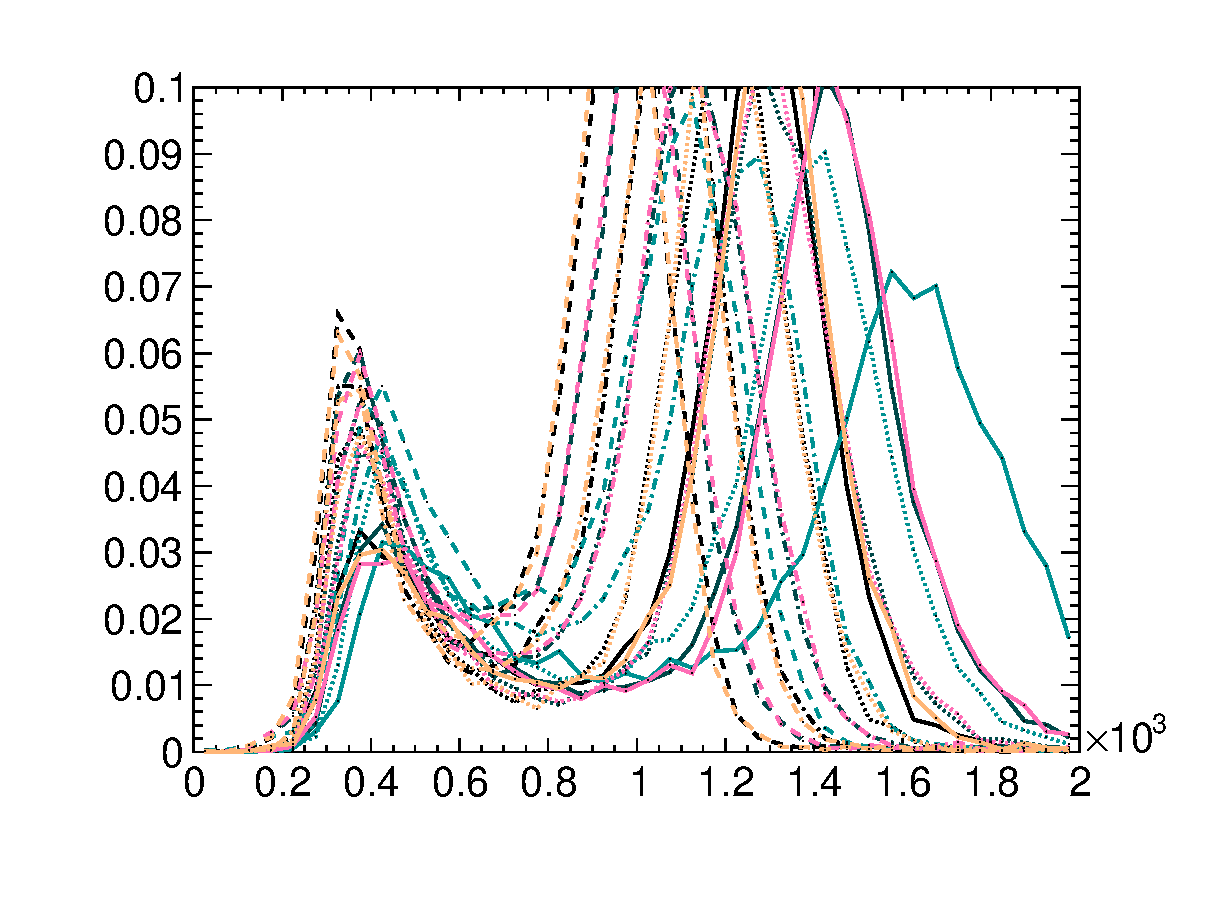
\includegraphics[width=\textwidth]{figures/sel/dedx5_pdf_skew_smooth.eps}
             \caption{Smoothed energy}
             \label{subfig:esc-smooth-e}
        \end{subfigure}
        \begin{subfigure}{\dbfigwid\textwidth}
             \centering
             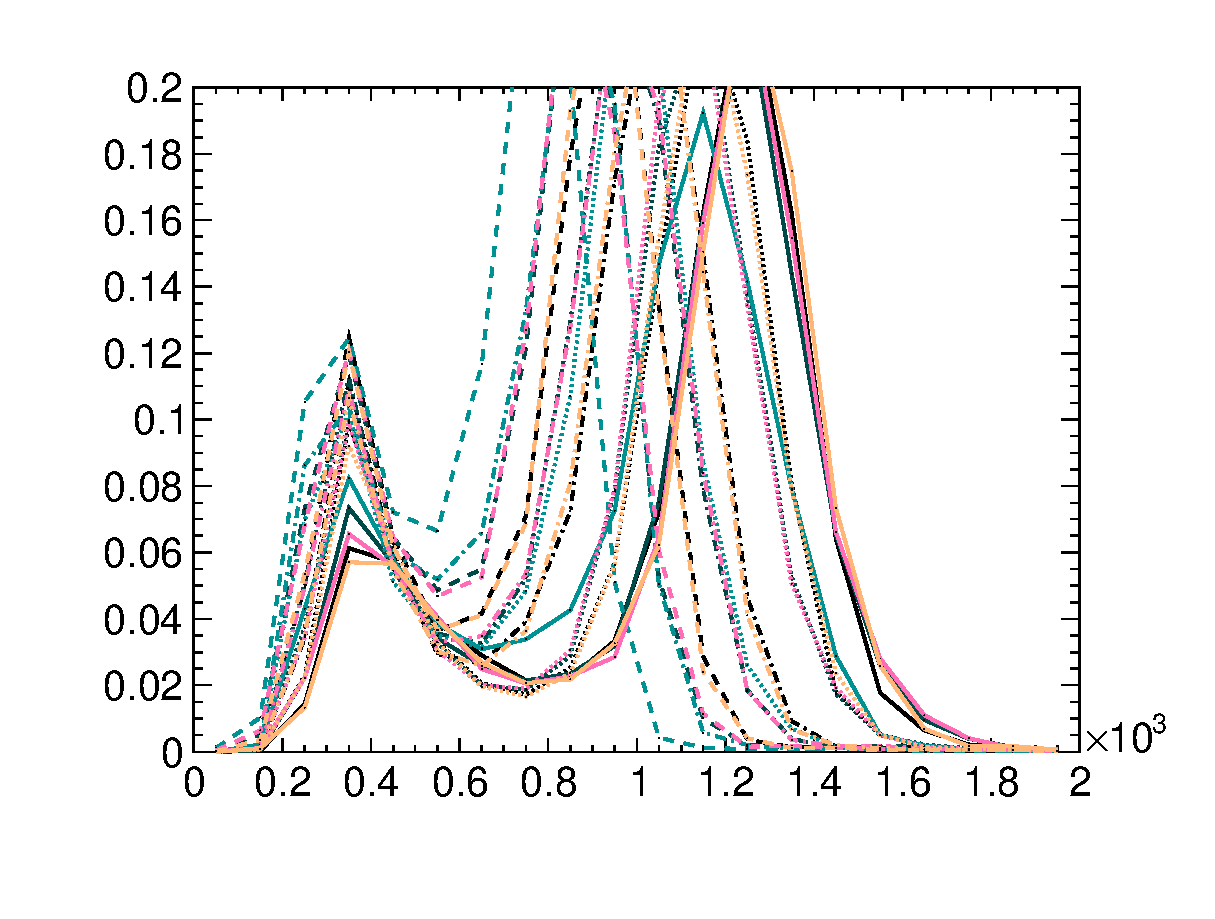
\includegraphics[width=\textwidth]{figures/sel/an_dedx5_pdf_skew_smooth_angnorm.eps}
             \caption{Angle-normalized smoothed energy}
             \label{subfig:esc-an-smooth-e}
        \end{subfigure}
        \caption{$\dedx$ estimation. Each colour represents a proton sample going in different directions. Each line style represents a different node from the end of the track. Altogether, there are 5 samples, each plotting for 4 nodes, resulting in 20 curves. Due to the large number of curves, the legend is omitted. The individual differences between the curves are not of interest here, but rather the overall agreement of the MIP peak positions across all curves can validate the quality of the estimation of $\dedx$. Fig.~\ref{subfig:esc-smooth-e} shows considerable spread in the MIP peak positions across different curves, while the MIP peak positions in Fig.~\ref{subfig:esc-an-smooth-e} are much closer across different curves. Therefore, the angle-normalized smoothed energy is a better estimate of $\dedx$ than the smoothed energy.}
        \label{fig:esc-angnorm}
     \end{figure}
     However, there are still some discrepancies.
     The MIP peaks are close to each other, but their positions differ noticeably.
     This is due to the different grouping of hits into nodes for protons travelling in different directions.
     The different numbers of hits in a node lead to different distances between nodes, so using the smoothed energy deposited per node as an estimation of $\dedx$ is not strictly valid.
     To account for the different propagation directions, I divided the energy by the sine of the angle between the trajectory and the $z$-axis.
     The angle-normalized energy is plotted in Fig.~\ref{subfig:esc-an-smooth-e}, which demonstrates that the angle-normalization step has achieved its goal—all MIP peaks have the similar position.
     Hence, the angle-normalized energy is used as a good reconstruction of $\dedx$ for the ESC selection, and it will be referred to as $\dedx$ in the following discussion.

     While the MIP peaks serve as a validation of the quality of the $\dedx$ estimation, the Bragg peaks are used to determine specific $\dedx$ thresholds for the ESC selection.
     To have a larger sample for threshold determination, the multiple PGUN samples are combined into one large sample.
     While plots like Fig.~\ref{fig:dedx-pprres-eg} show the underlying idea of the ESC selection, profile plots are better suited for determining proper thresholds.
     Hence, the profile plots of $\dedx$ for the last six nodes at the end of the proton track are collected in Fig.~\ref{fig:esc-andedx-slice}.
     To simplify the discussion, the $\dedx$ at the last node is referred to as $\dedx_1$, the second last node as $\dedx_2$, and so on, up to the sixth last node as $\dedx_6$.
     For example, Fig.~\ref{subfig:ans-dedx0-ppr-slice} shows considerably larger fluctuations in reconstruction quality when $\dedx_1$ falls below $200$, where a cut should be placed to exclude these events.
     Similarly, the threshold values from $\dedx_2$ to $\dedx_6$ are extracted to be $500$, $1000$, $900$, $840$, and $740$ respectively.

  \begin{figure}[!htb]
      \centering
      \begin{subfigure}[!htb]{\dbfigwid\textwidth}
          %  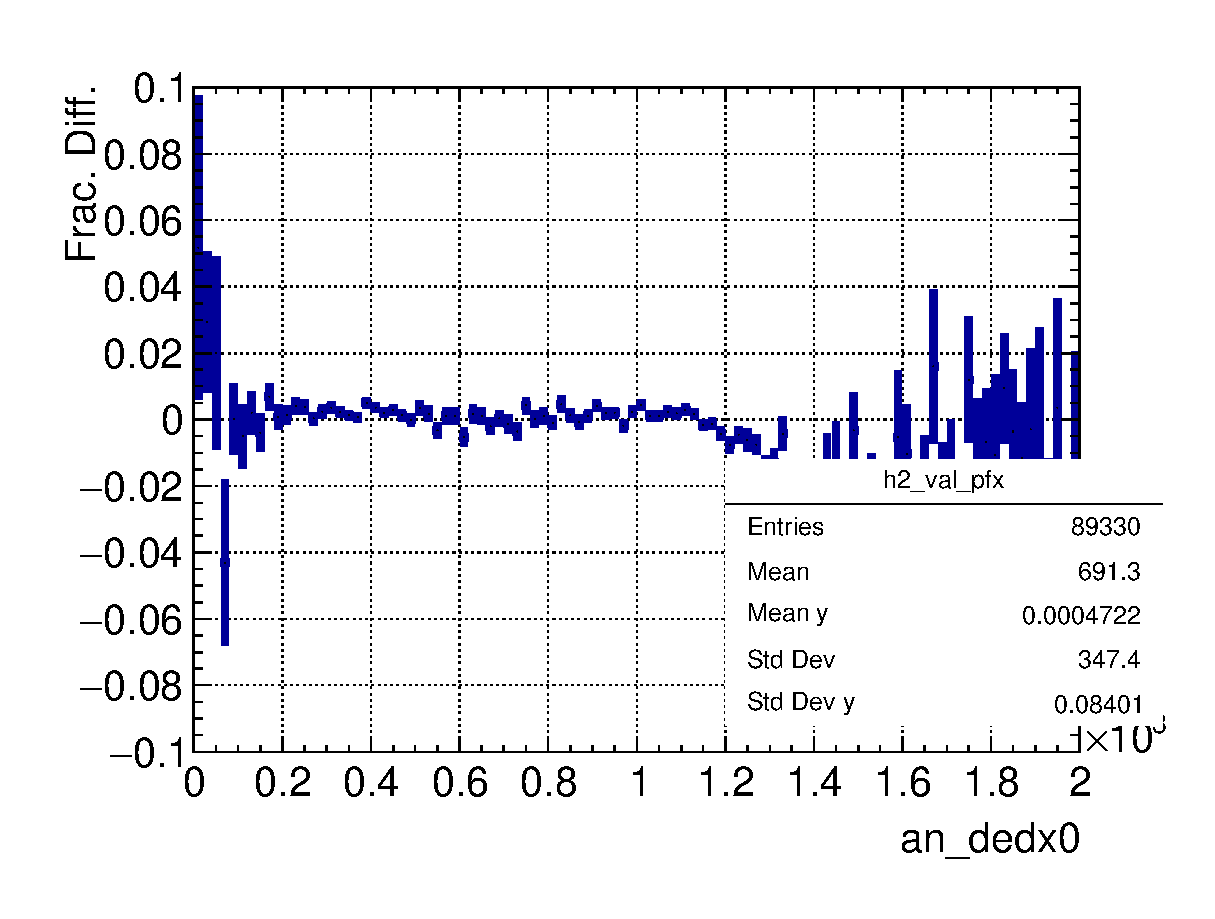
\includegraphics[width=\textwidth]{figures/sel/ans_dedx0_vs_p_pr_res_hist2d_al2_selpr_con_slice.eps}
           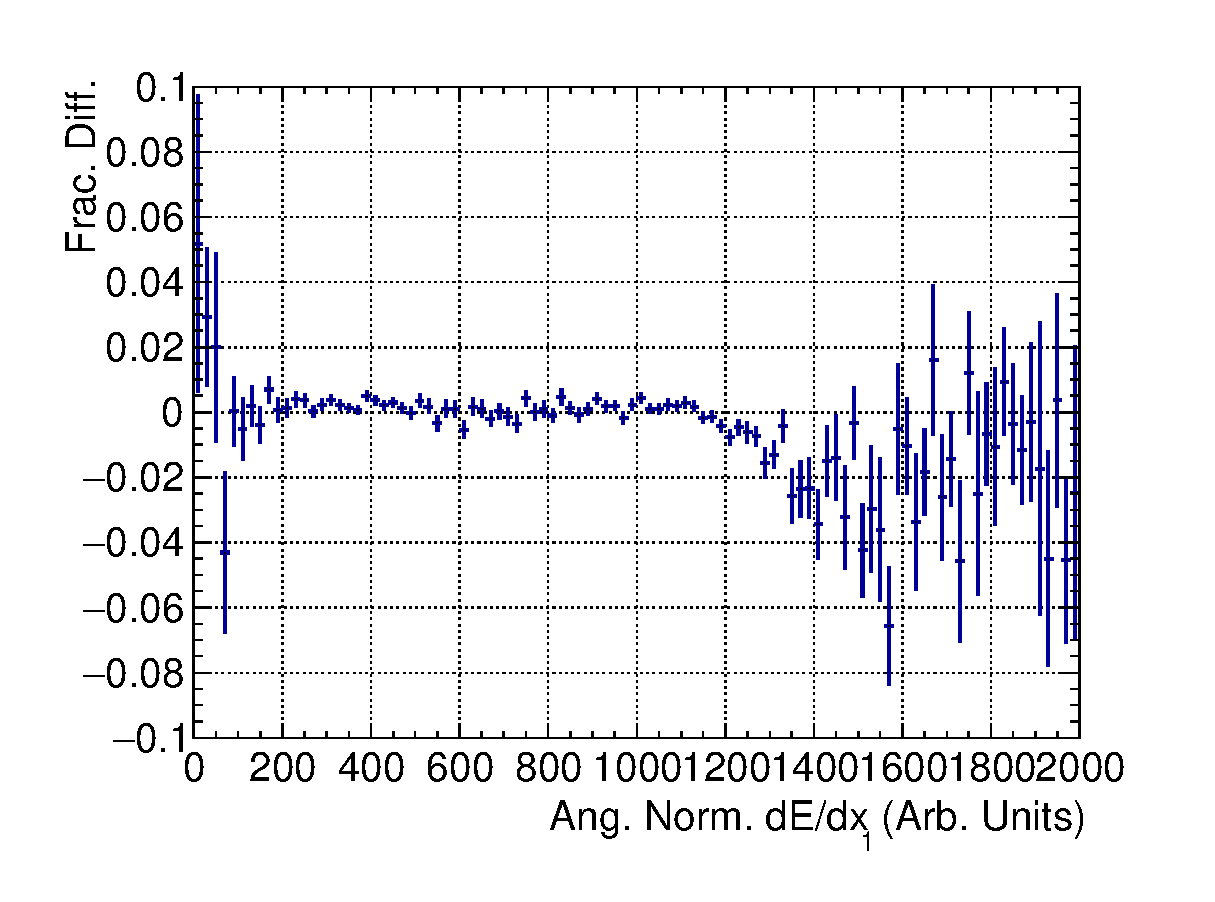
\includegraphics[width=\textwidth]{figures/sel/fig53a.eps}
           \caption{$\dedx_1$, considerably larger fluctuations in reconstruction quality when $\dedx_1$ falls below $200$.}
           \label{subfig:ans-dedx0-ppr-slice}
      \end{subfigure}
      \begin{subfigure}[!htb]{\dbfigwid\textwidth}
          %  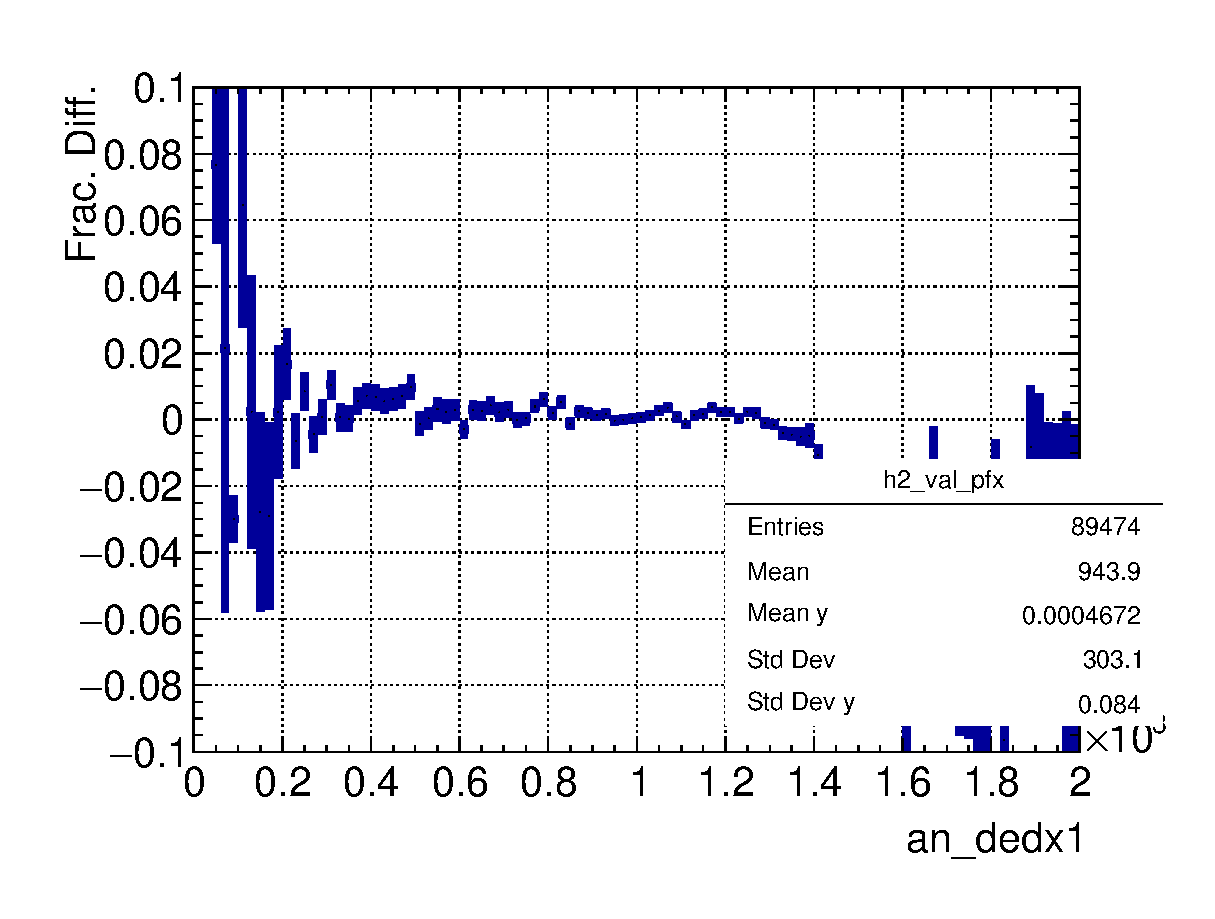
\includegraphics[width=\textwidth]{figures/sel/ans_dedx1_vs_p_pr_res_hist2d_al2_selpr_con_slice.eps}
           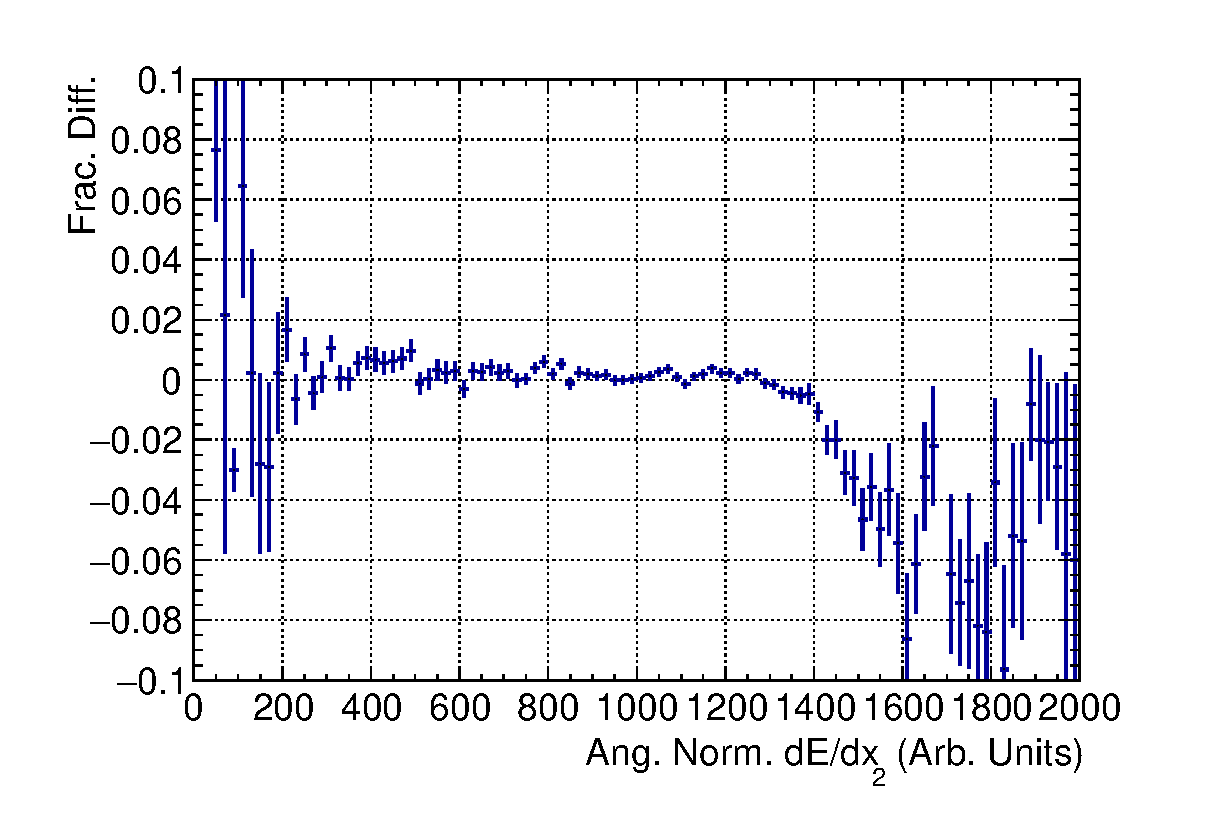
\includegraphics[width=\textwidth]{figures/sel/fig53b.eps}
           \caption{$\dedx_2$, considerably larger fluctuations in reconstruction quality when $\dedx_2$ falls below $500$.}
           \label{subfig:dedx1}
      \end{subfigure}
      \\
      \begin{subfigure}[!htb]{\dbfigwid\textwidth}
           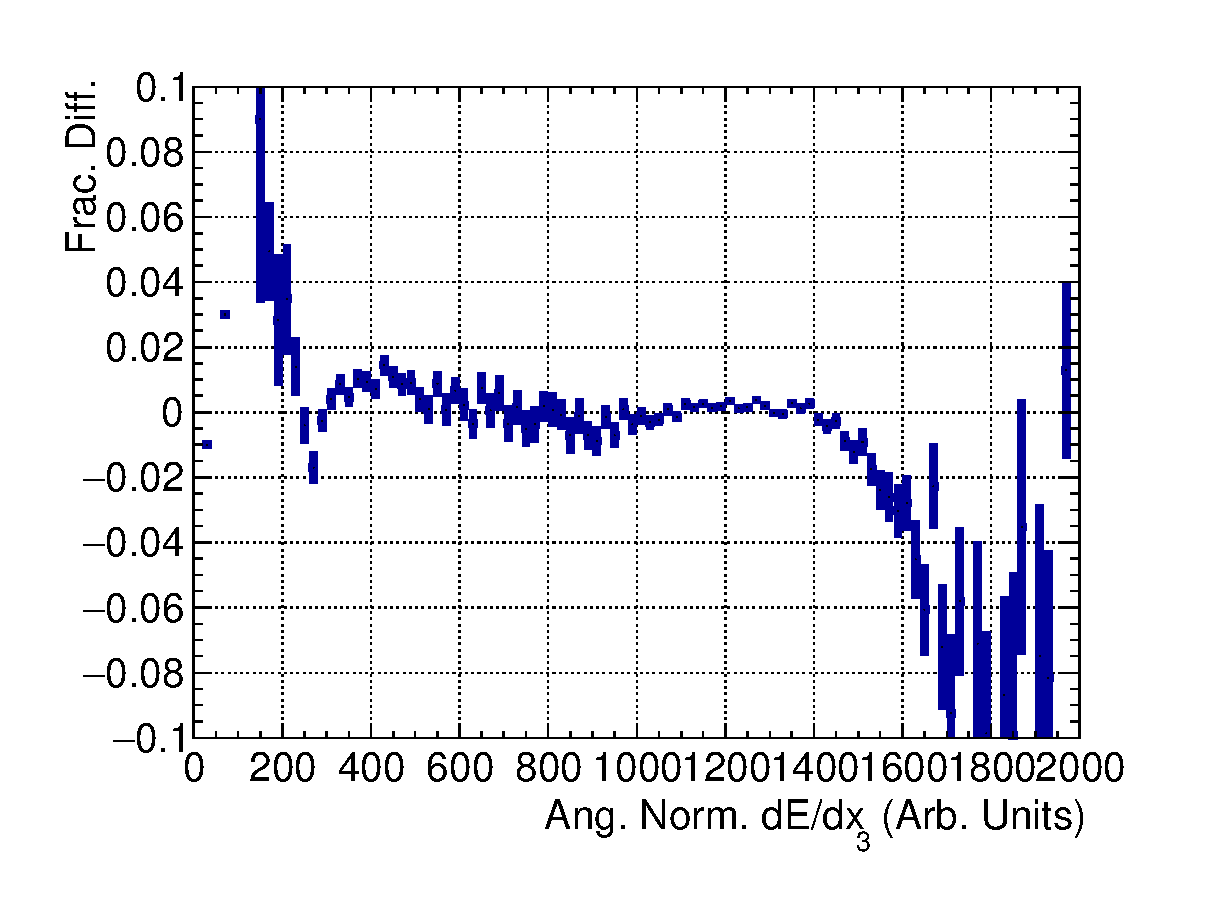
\includegraphics[width=\textwidth]{figures/sel/fig53c.eps}
          %  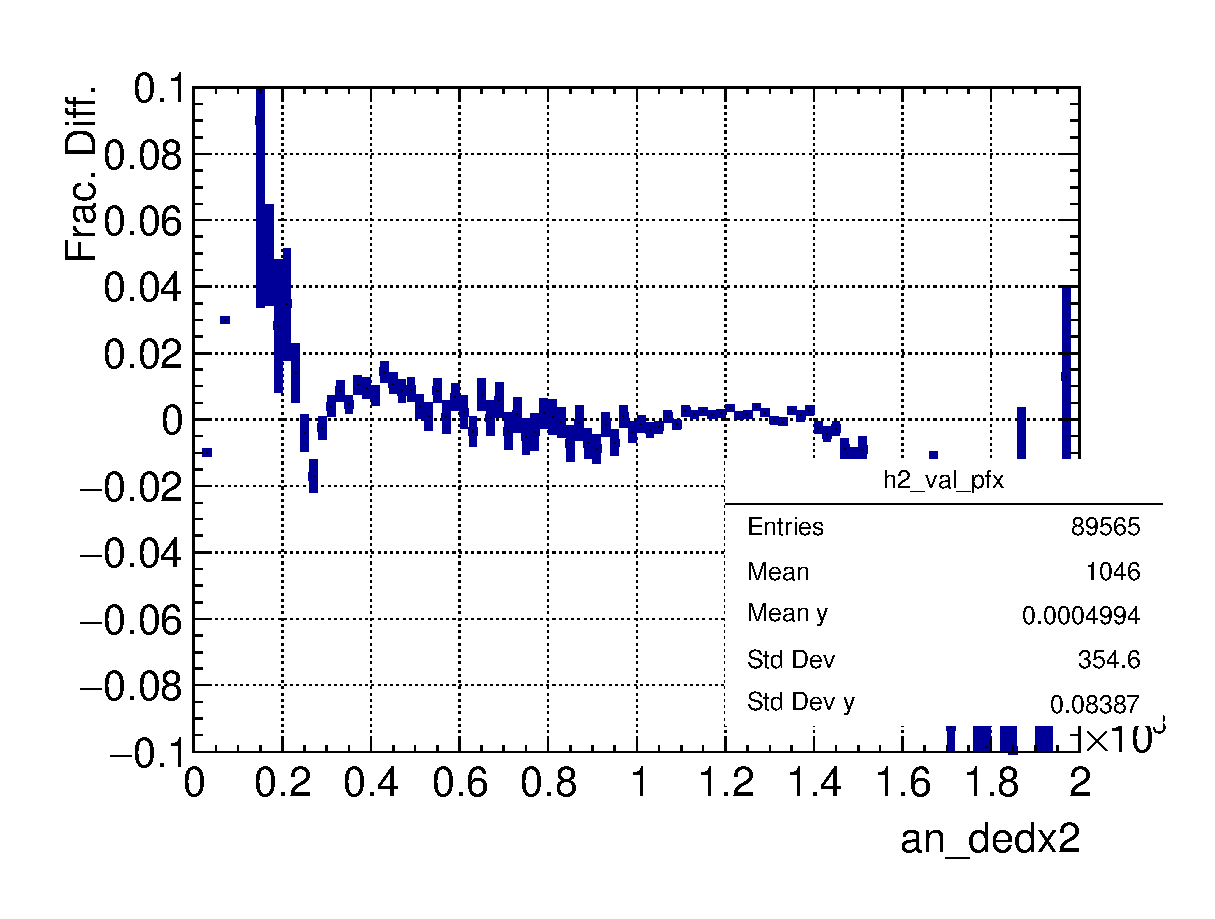
\includegraphics[width=\textwidth]{figures/sel/ans_dedx2_vs_p_pr_res_hist2d_al2_selpr_con_slice.eps}
           \caption{$\dedx_3$, considerably larger fluctuations in reconstruction quality when $\dedx_3$ falls below $1000$.}
           \label{subfig:dedx2}
      \end{subfigure}
      \begin{subfigure}{\dbfigwid\textwidth}
          %  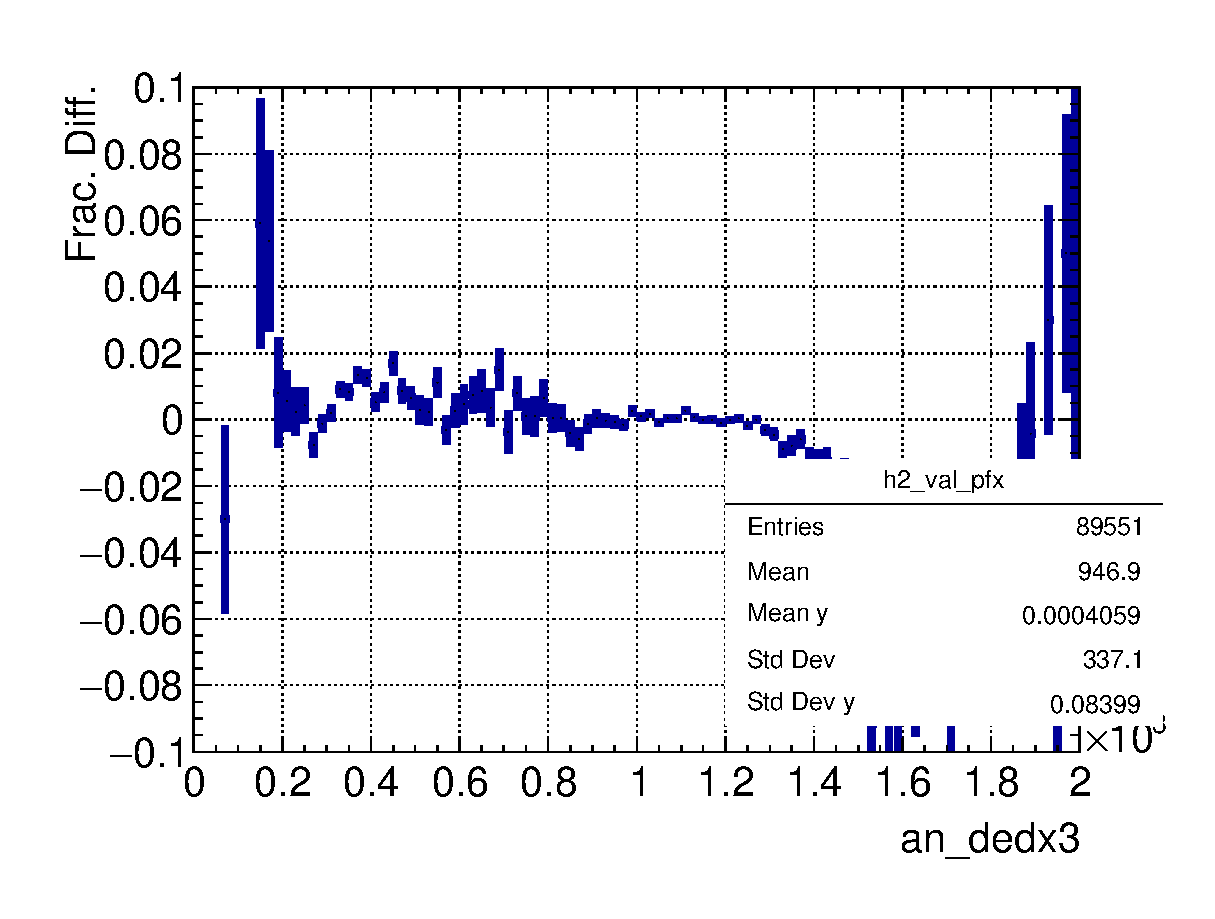
\includegraphics[width=\textwidth]{figures/sel/ans_dedx3_vs_p_pr_res_hist2d_al2_selpr_con_slice.eps}
           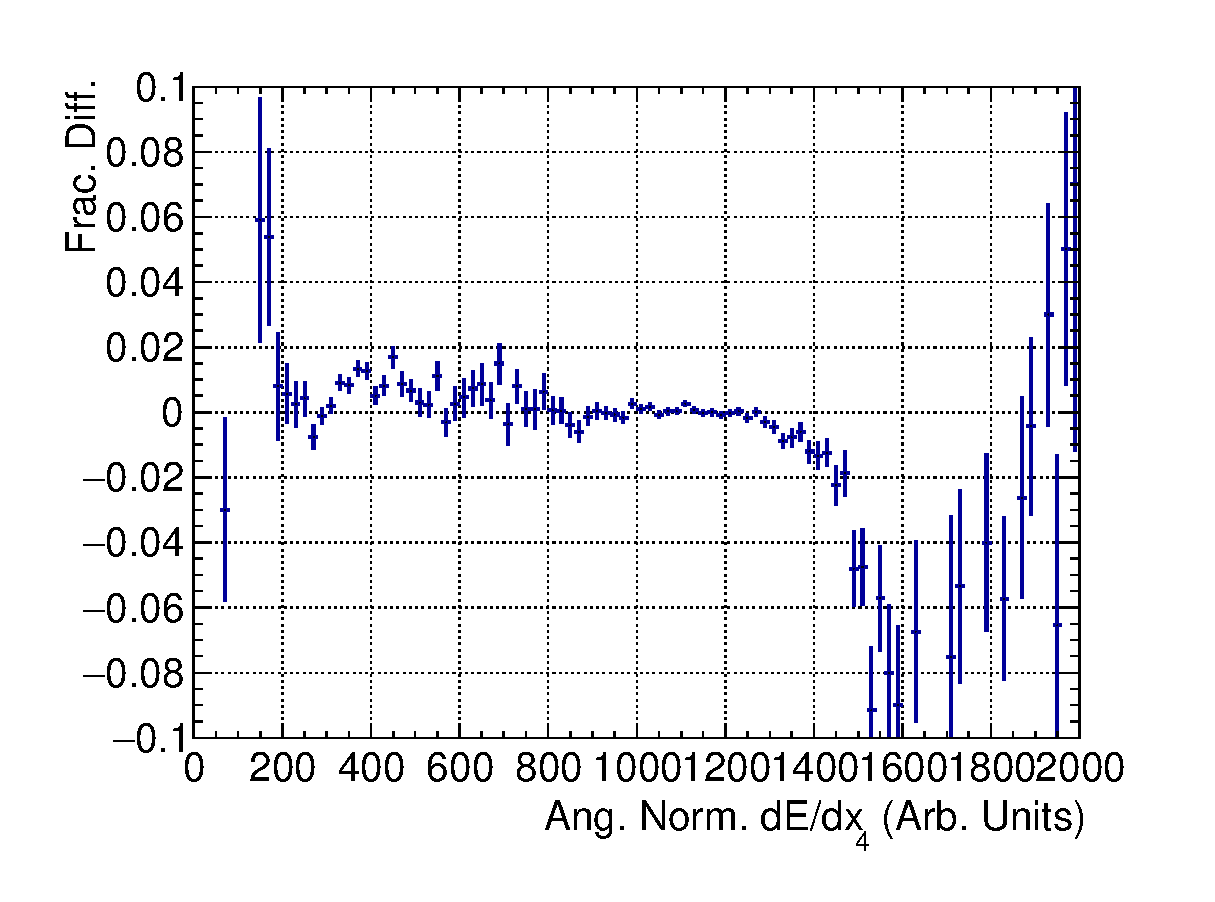
\includegraphics[width=\textwidth]{figures/sel/fig53d.eps}
           \caption{$\dedx_4$, considerably larger fluctuations in reconstruction quality when $\dedx_4$ falls below $900$.}
           \label{subfig:dedx3}
      \end{subfigure}
      \\
      \begin{subfigure}[!htb]{\dbfigwid\textwidth}
          %  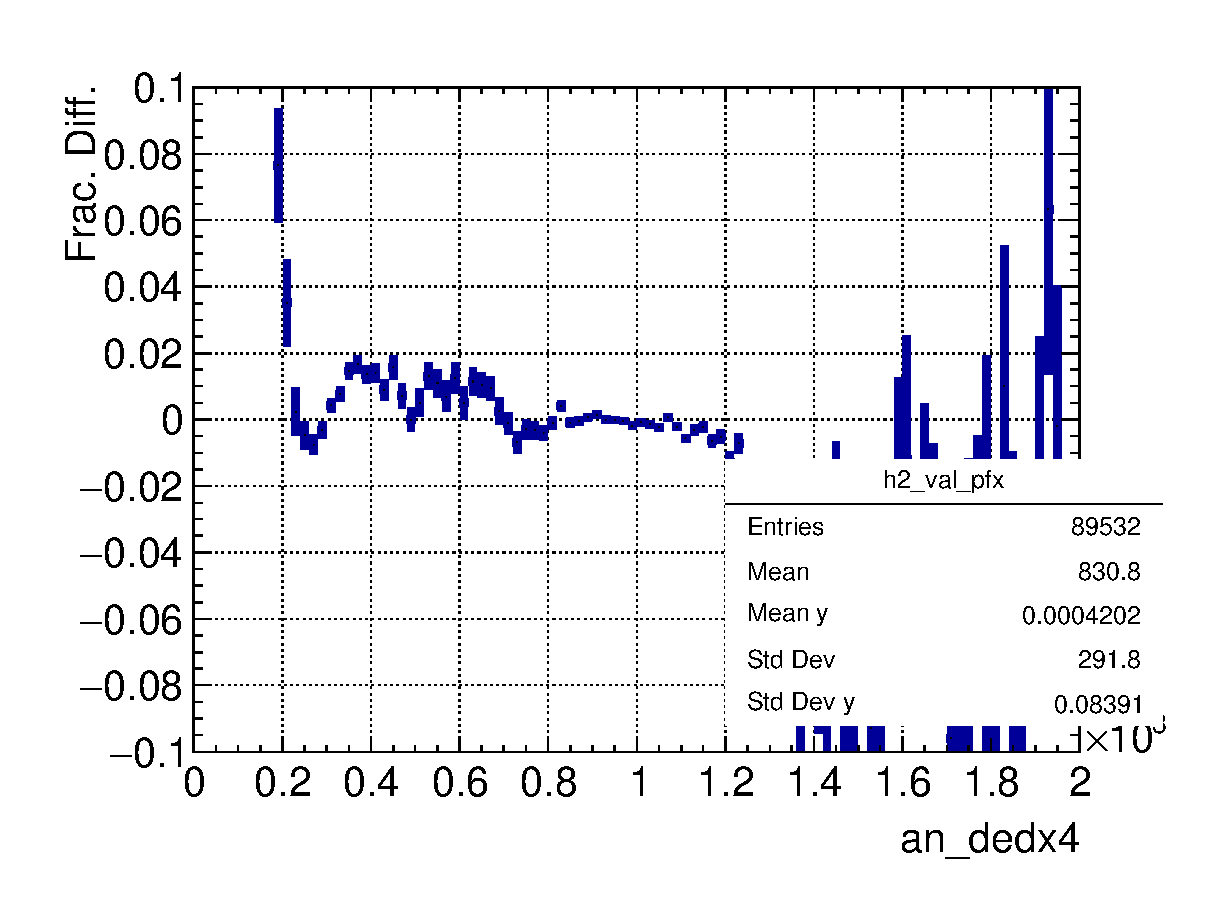
\includegraphics[width=\textwidth]{figures/sel/ans_dedx4_vs_p_pr_res_hist2d_al2_selpr_con_slice.eps}
           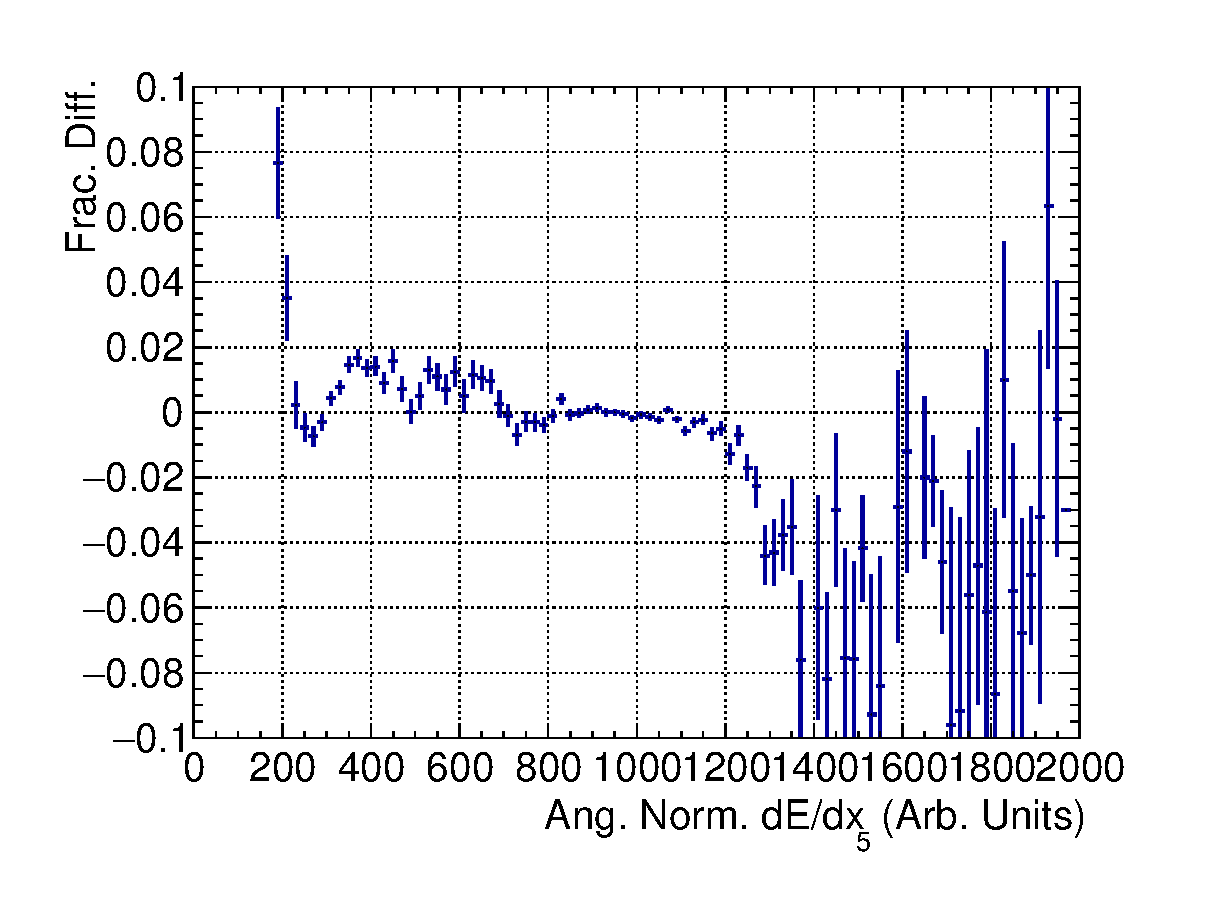
\includegraphics[width=\textwidth]{figures/sel/fig53e.eps}
           \caption{$\dedx_5$, considerably larger fluctuations in reconstruction quality when $\dedx_5$ falls below $840$.}
           \label{subfig:dedx4}
      \end{subfigure}
      \begin{subfigure}[!htb]{\dbfigwid\textwidth}
          %  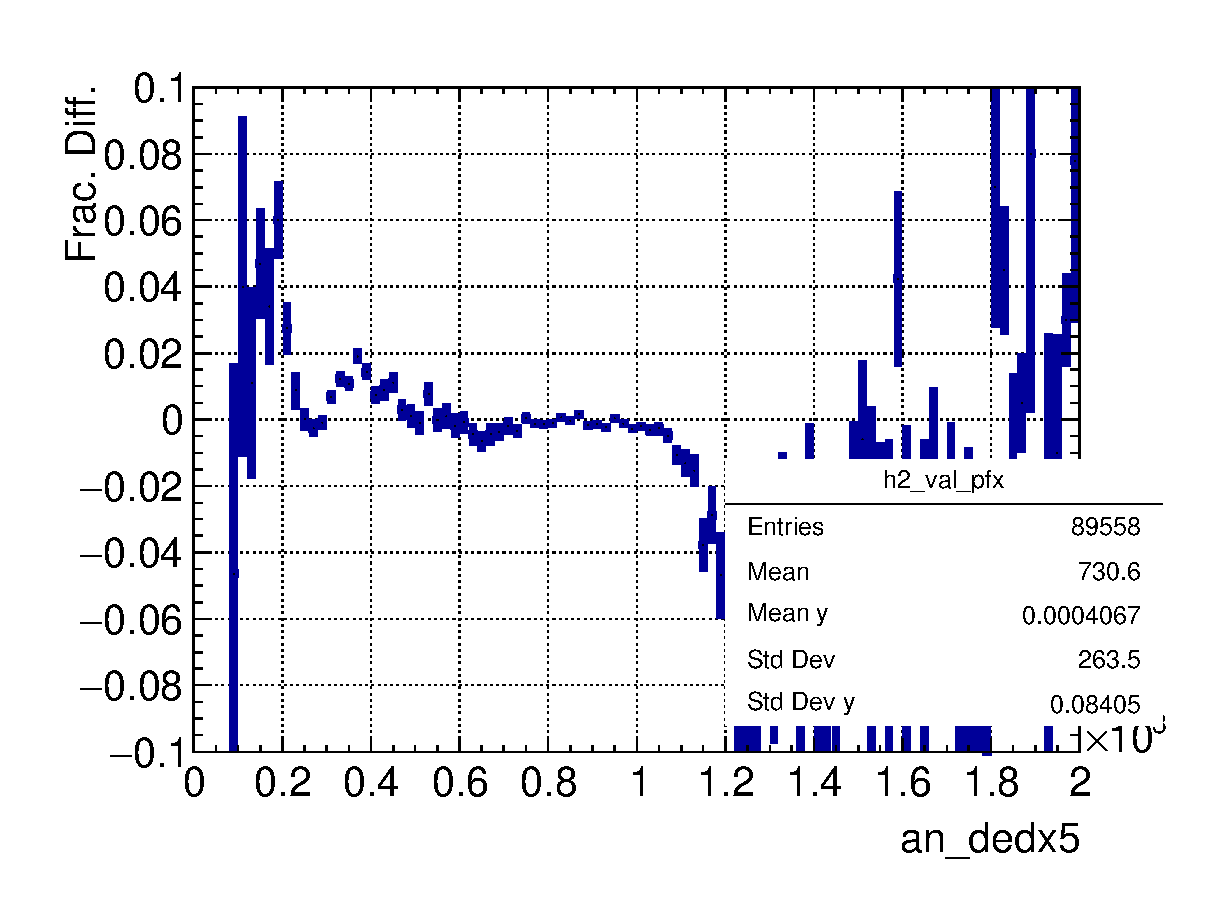
\includegraphics[width=\textwidth]{figures/sel/ans_dedx5_vs_p_pr_res_hist2d_al2_selpr_con_slice.eps}
           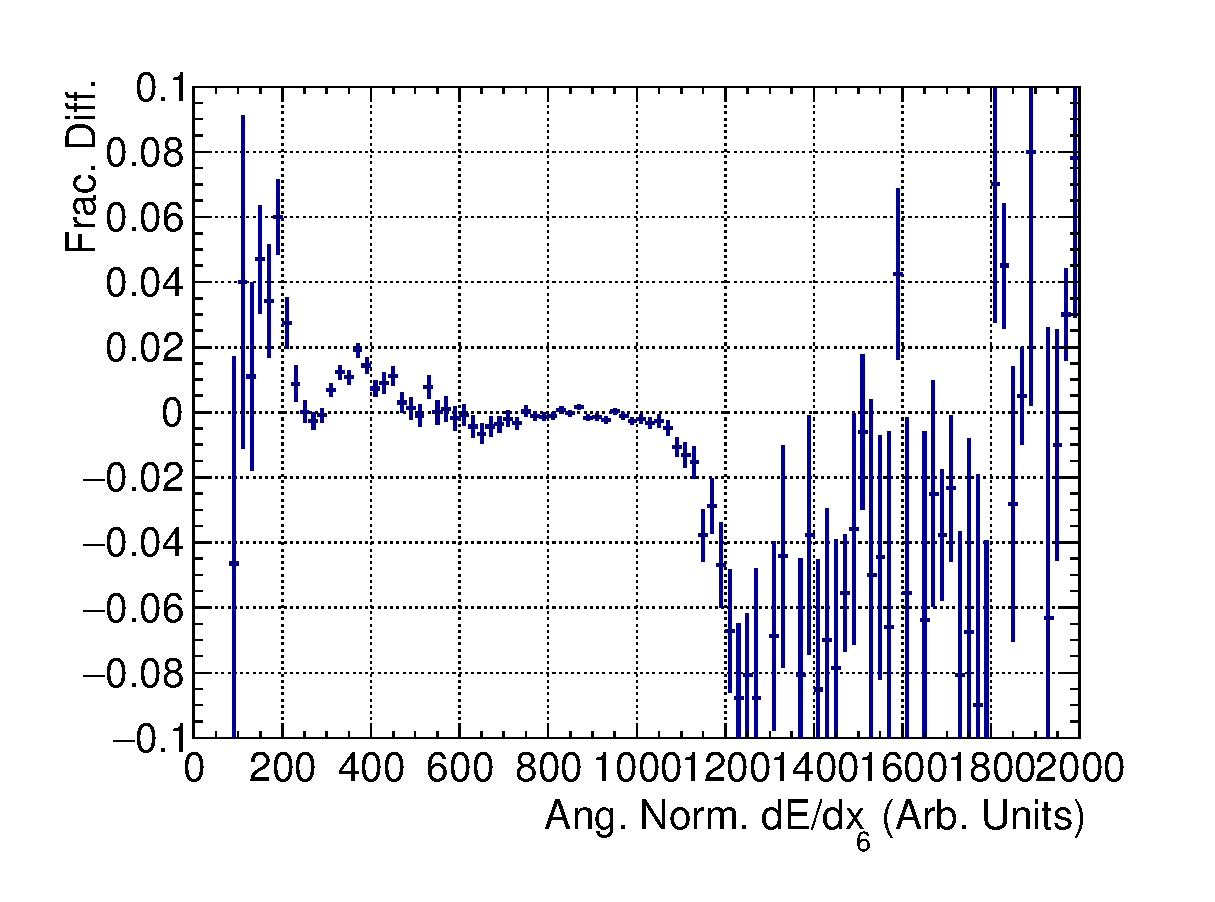
\includegraphics[width=\textwidth]{figures/sel/fig53f.eps}
           \caption{$\dedx_6$, considerably larger fluctuations in reconstruction quality when $\dedx_6$ falls below $740$.}
           \label{subfig:dedx5}
      \end{subfigure}
      \caption{Proton momentum reconstruction fractional difference against $\dedx$ for determination of $\dedx$ thresholds. The corresponding thresholds values are extracted in each subfigure.}
      \label{fig:esc-andedx-slice}
  \end{figure}

     Furthermore, based on the $6$ distributions of $\dedx$, the average Bragg peak profile can be obtained by fitting the peaks of these distributions.
     Fig.~\ref{fig:esc-andedx-peaks} shows the $\dedx$ distributions for the last six nodes of the proton track.
     The specific $\dedx$ values constituting the Bragg peak are extracted by fitting the distributions with a Cauchy function near the peak region.
     Note that the fit is used to extract the peak value, not to model the entire distribution, so the fit quality is not of primary concern.
     From $\dedx_1$ to $\dedx_6$, the fitted Bragg peak values are $989.5$, $1080$, $1234$, $1131$, $990.0$, and $887.2$, respectively.

  \begin{figure}[ht]
    \centering
    \begin{subfigure}{\dbfigwid\textwidth}
     %     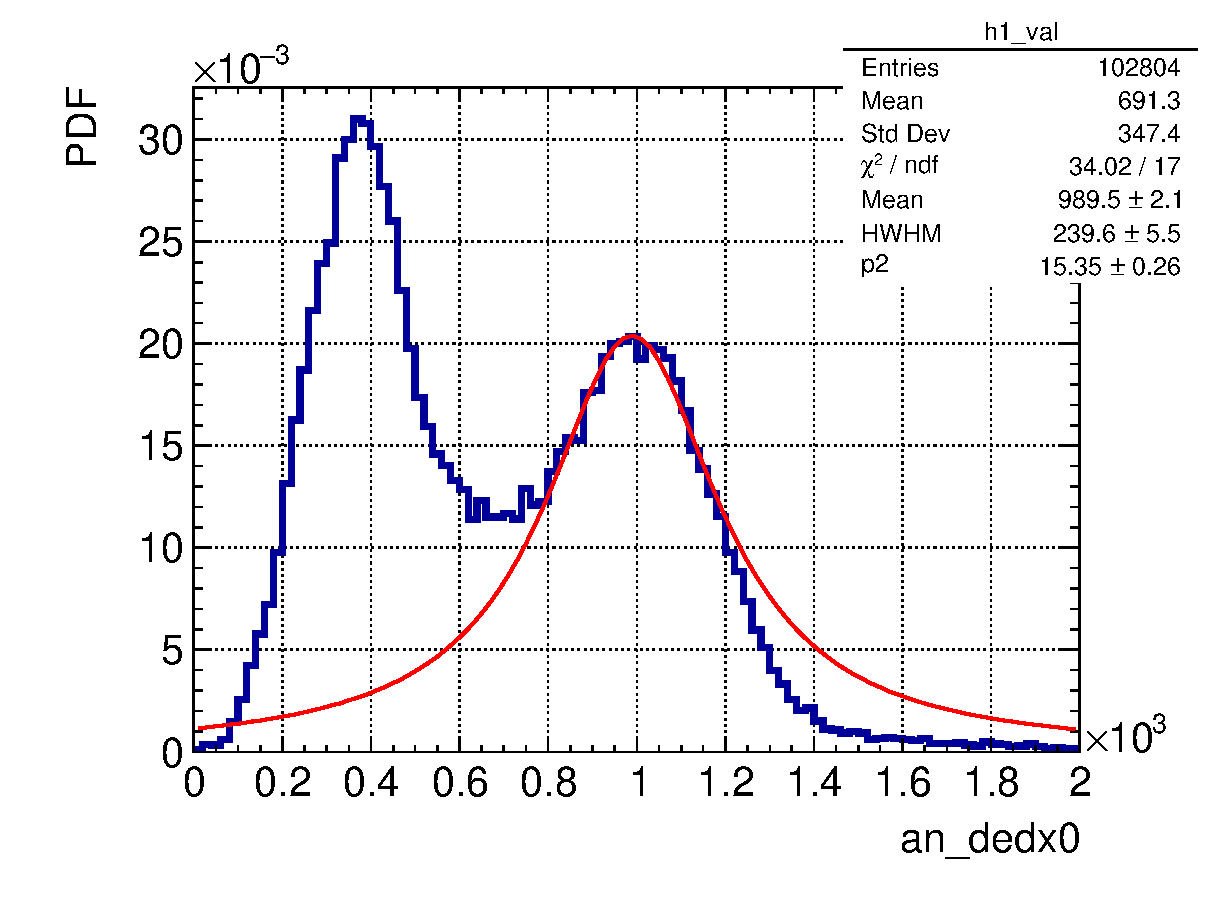
\includegraphics[width=\textwidth]{figures/sel/ans_dedx0_pdf_al2_selpr_con_test.eps}
         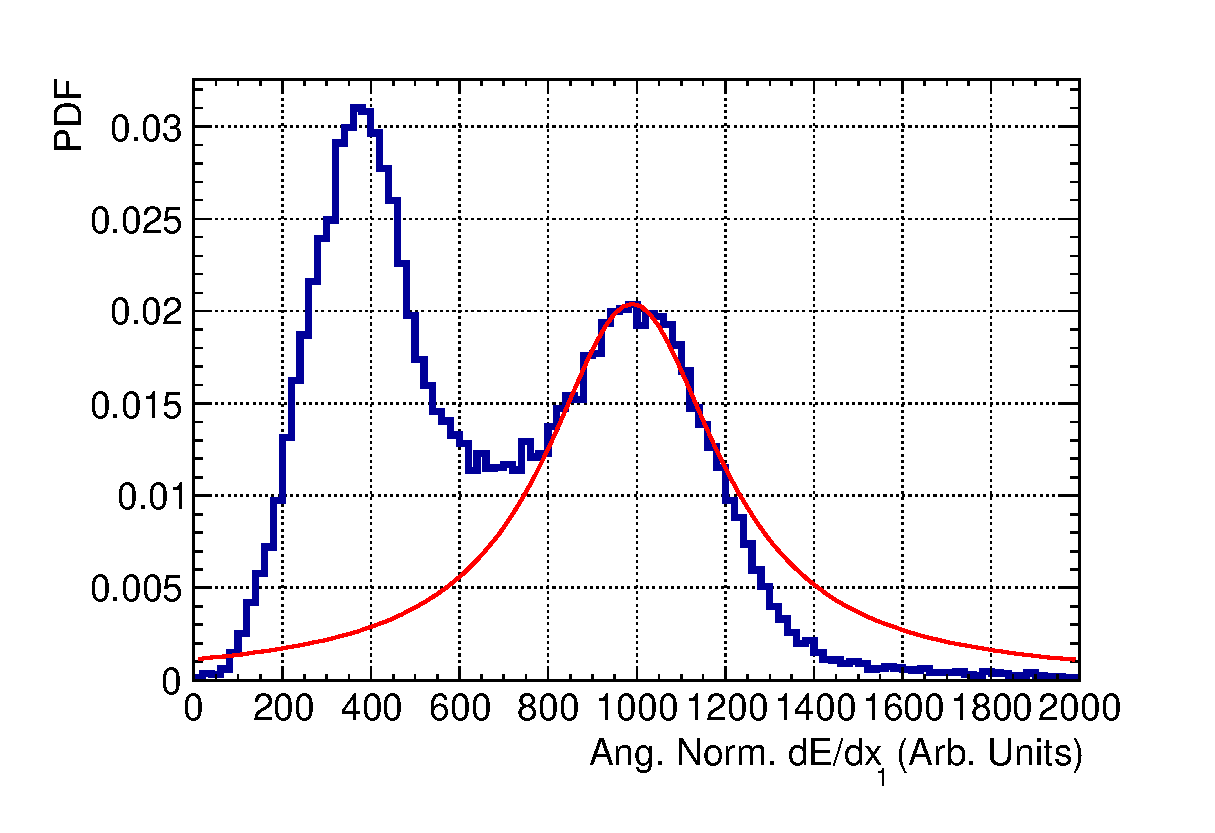
\includegraphics[width=\textwidth]{figures/sel/fig54a.eps}
         \caption{$\dedx_1$ Bragg peak value fit. The fitted peak value is $989.5$.}
         \label{subfig:dedx0-peak}
    \end{subfigure}
    \begin{subfigure}{\dbfigwid\textwidth}
     %     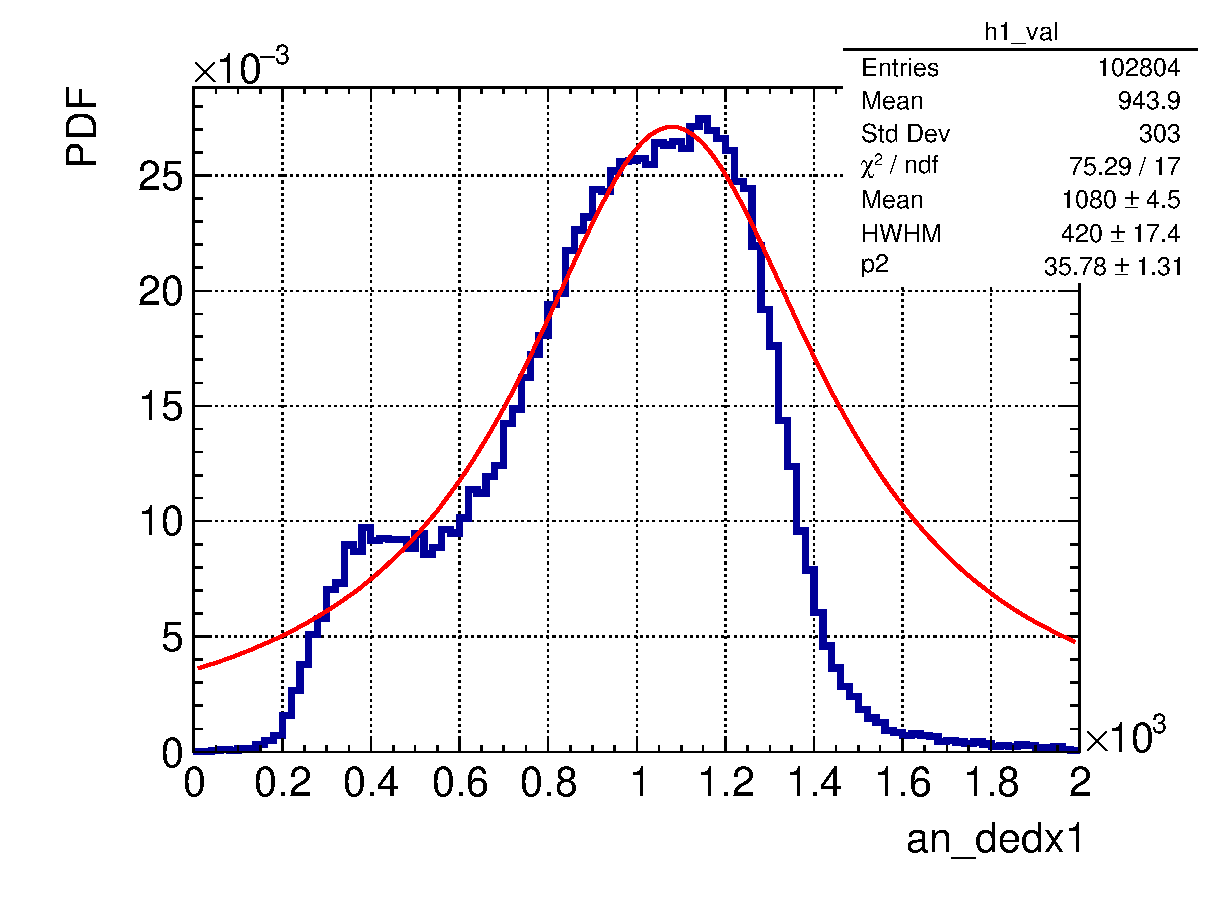
\includegraphics[width=\textwidth]{figures/sel/ans_dedx1_pdf_al2_selpr_con_test.eps}
         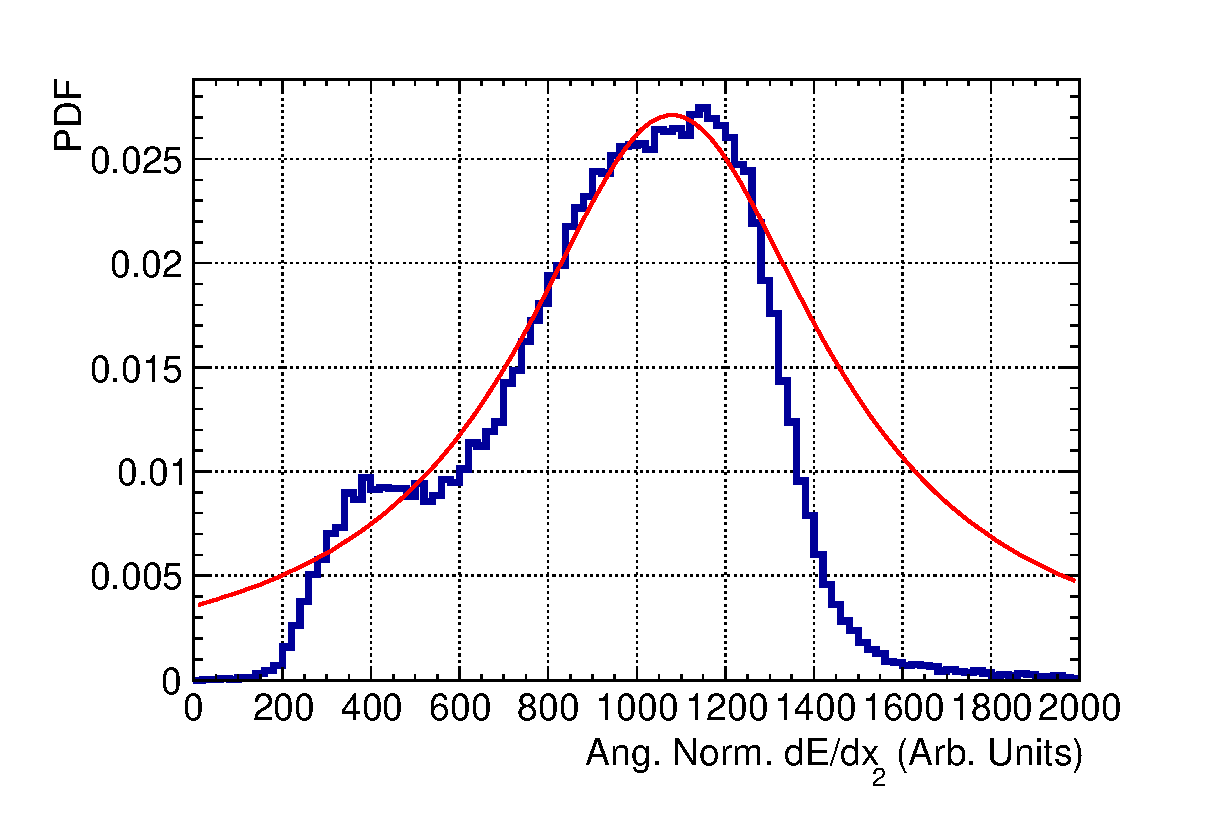
\includegraphics[width=\textwidth]{figures/sel/fig54b.eps}
         \caption{$\dedx_2$ Bragg peak value fit. The fitted peak value is $1080$.}
         \label{subfig:dedx1-peak}
    \end{subfigure}
    \\
    \begin{subfigure}{\dbfigwid\textwidth}
     %     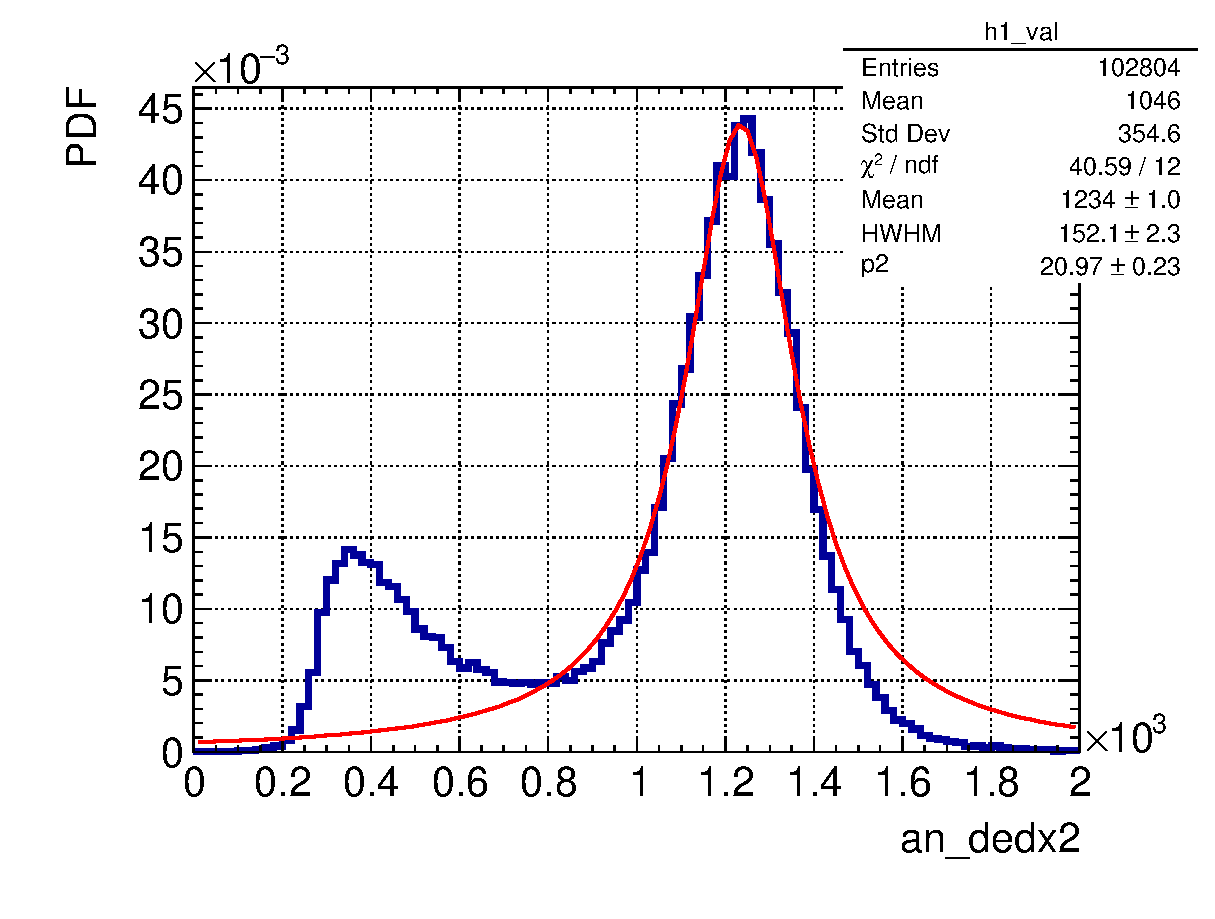
\includegraphics[width=\textwidth]{figures/sel/ans_dedx2_pdf_al2_selpr_con_test.eps}
         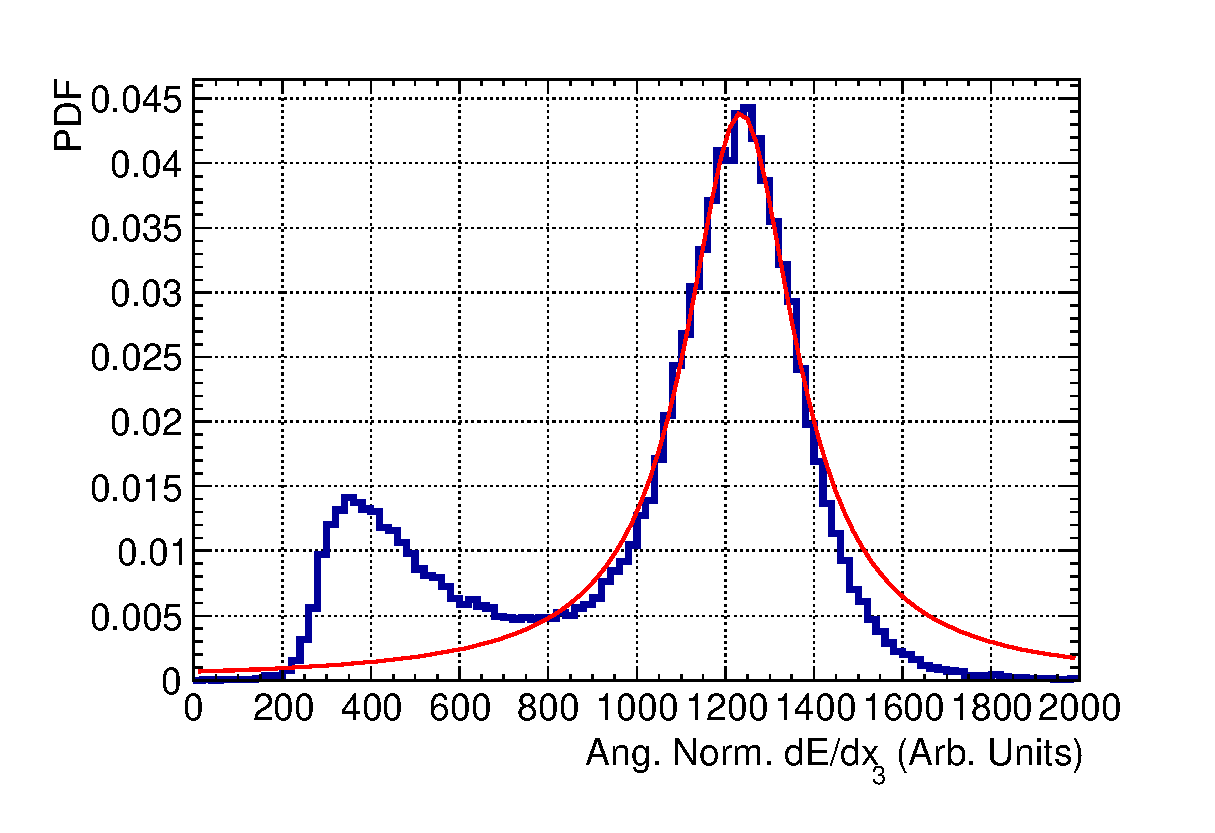
\includegraphics[width=\textwidth]{figures/sel/fig54c.eps}
         \caption{$\dedx_3$ Bragg peak value fit. The fitted peak value is $1234$.}
         \label{subfig:dedx2-peak}
    \end{subfigure}
    \begin{subfigure}{\dbfigwid\textwidth}
     %     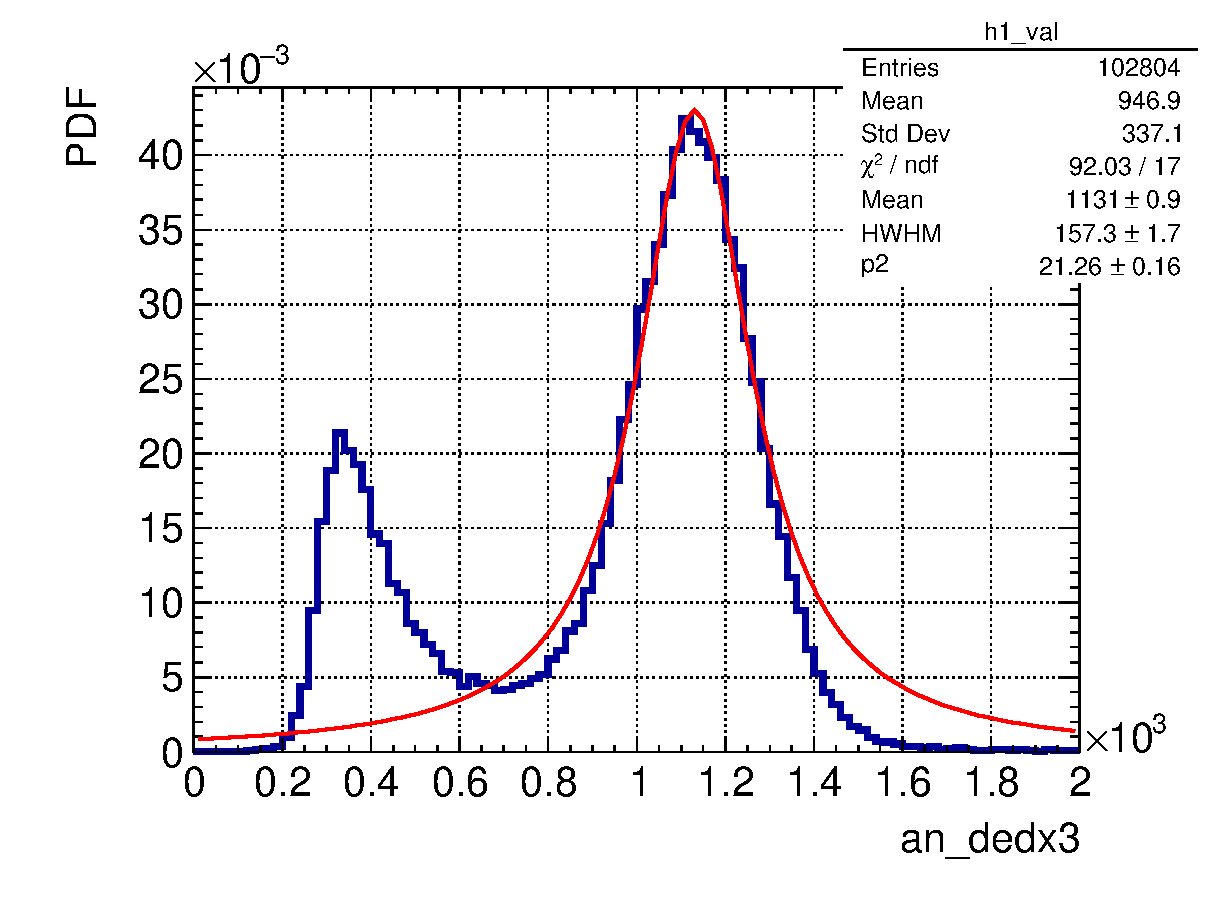
\includegraphics[width=\textwidth]{figures/sel/ans_dedx3_pdf_al2_selpr_con_test.eps}
         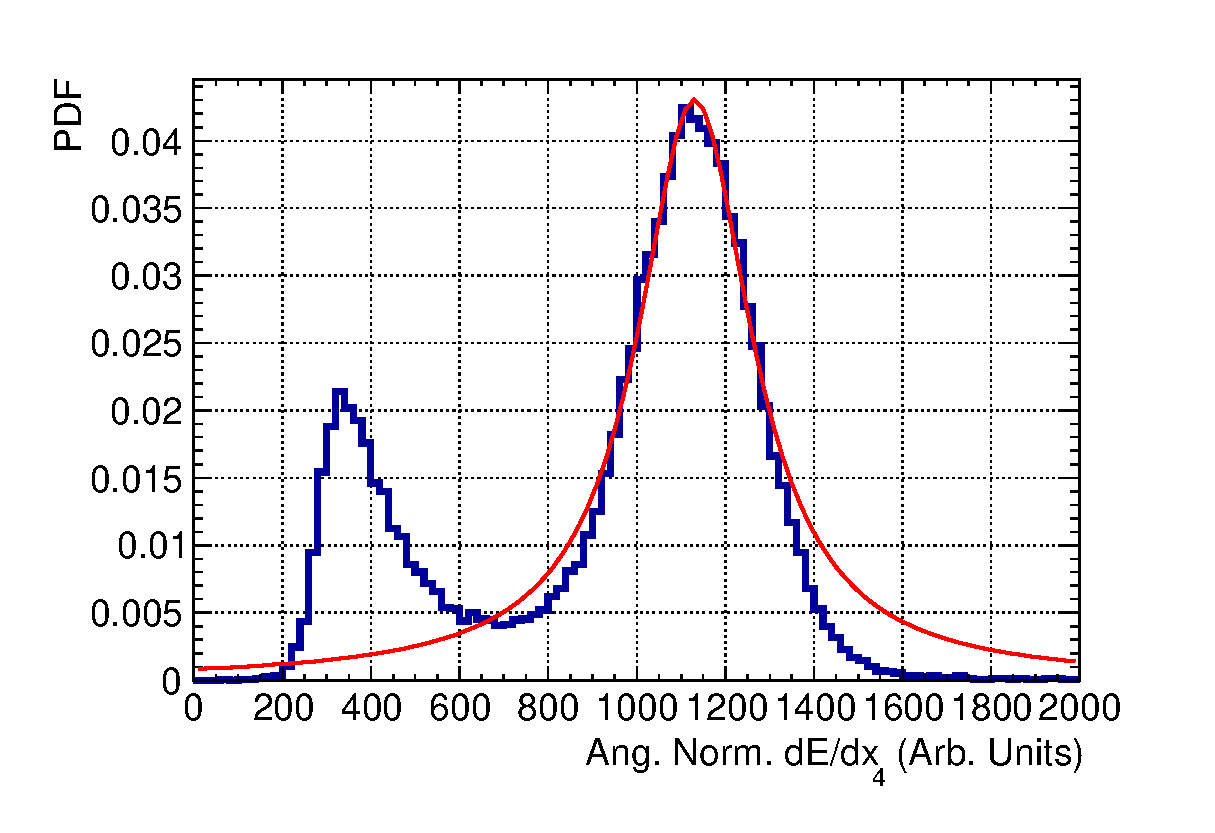
\includegraphics[width=\textwidth]{figures/sel/fig54d.eps}
         \caption{$\dedx_4$ Bragg peak value fit. The fitted peak value is $1131$.}
         \label{subfig:dedx3-peak}
    \end{subfigure}
    \\
    \begin{subfigure}{\dbfigwid\textwidth}
     %     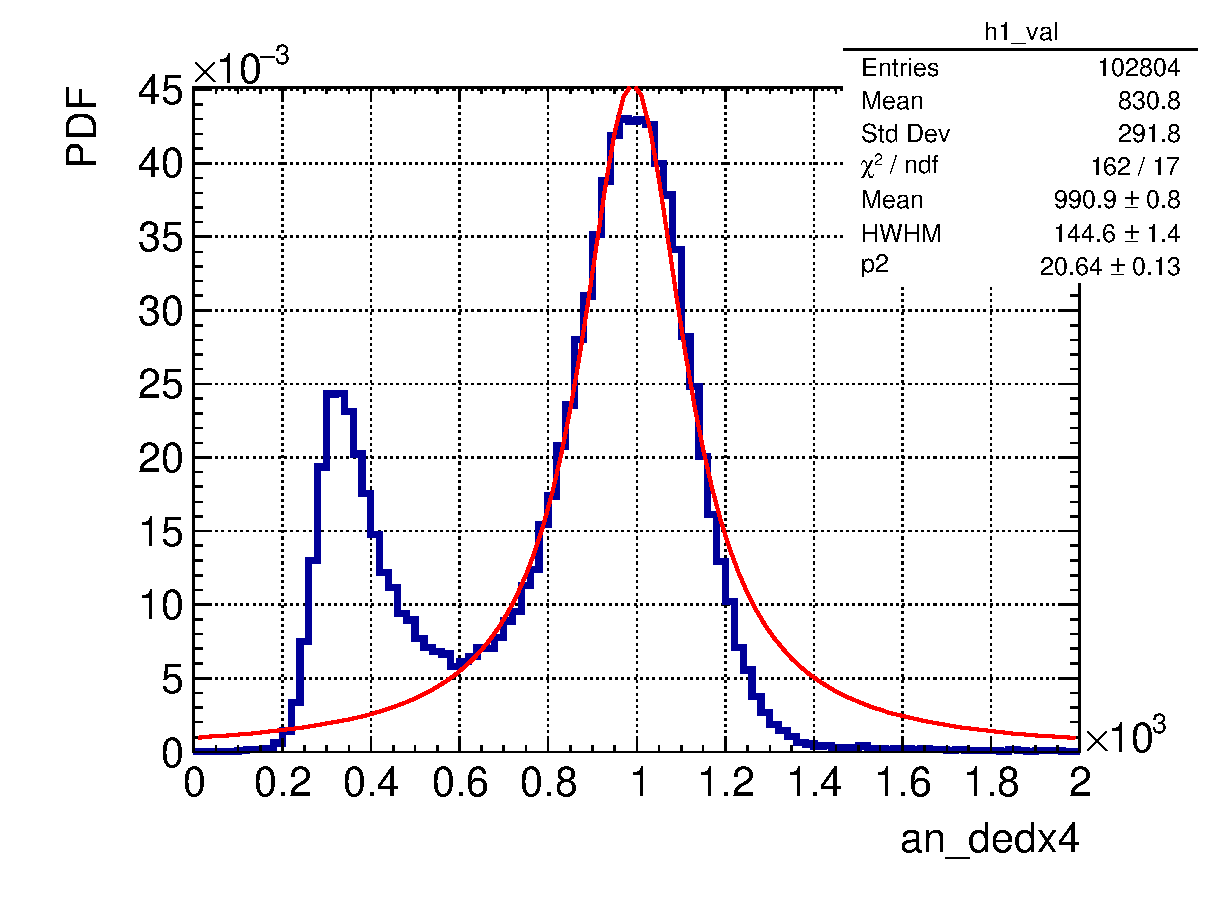
\includegraphics[width=\textwidth]{figures/sel/ans_dedx4_pdf_al2_selpr_con_test.eps}
         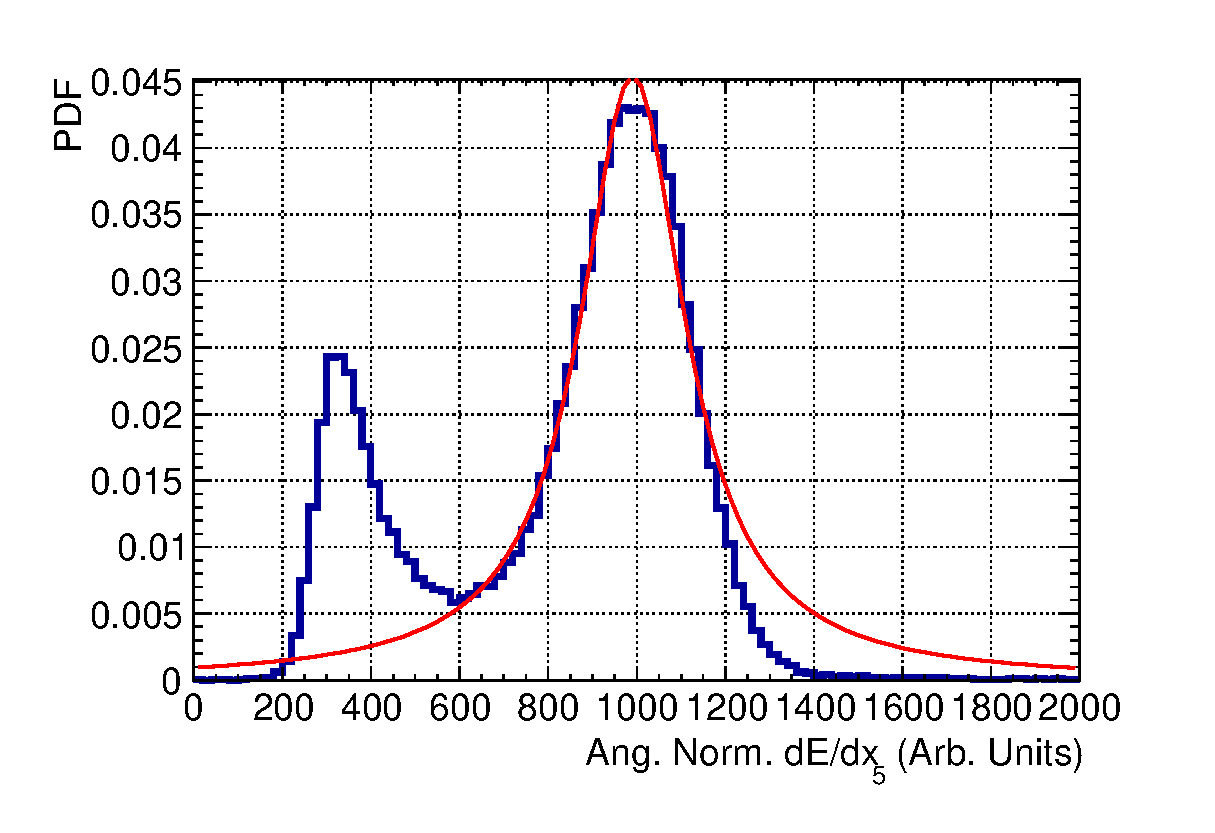
\includegraphics[width=\textwidth]{figures/sel/fig54e.eps}
         \caption{$\dedx_5$ Bragg peak value fit. The fitted peak value is $990.0$.}
         \label{subfig:dedx4-peak}
    \end{subfigure}
    \begin{subfigure}{\dbfigwid\textwidth}
     %     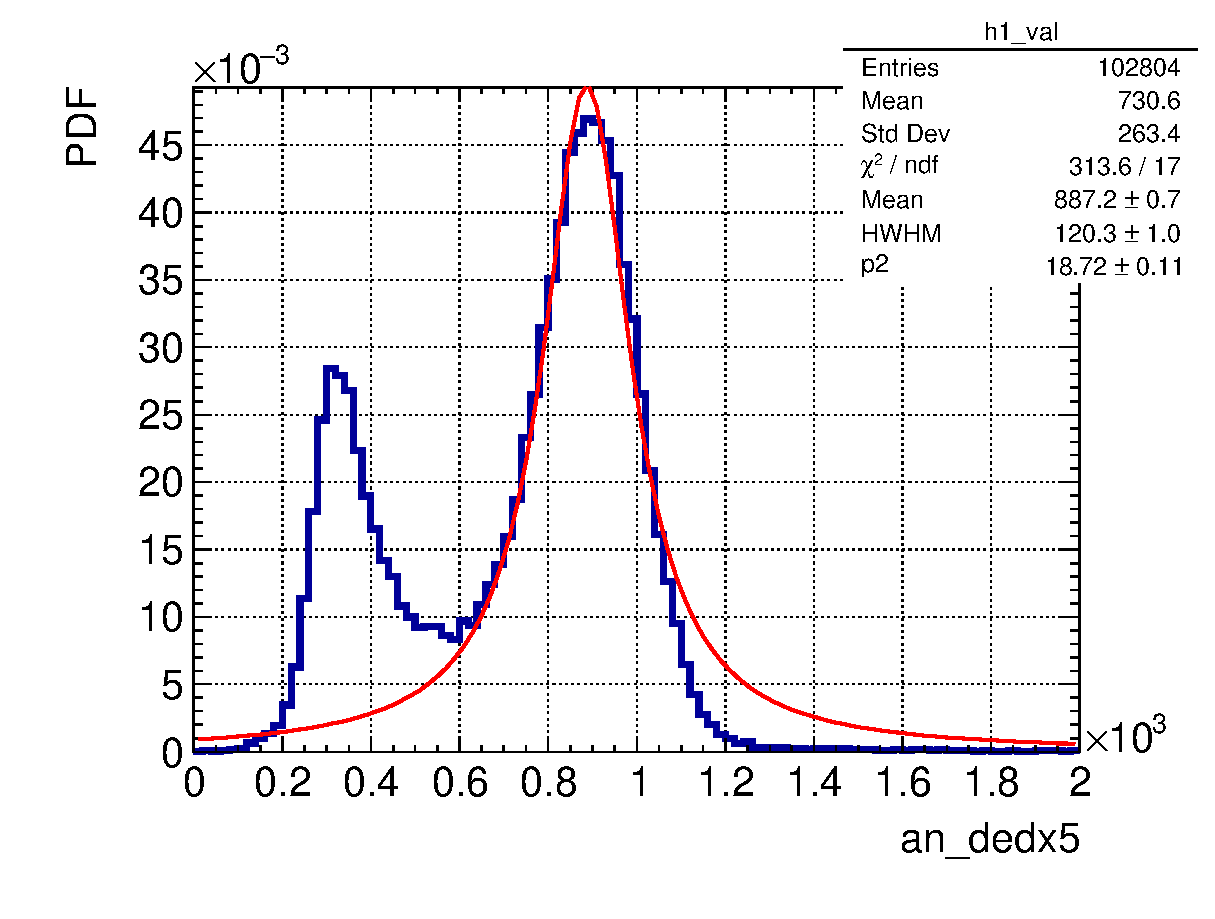
\includegraphics[width=\textwidth]{figures/sel/ans_dedx5_pdf_al2_selpr_con_test.eps}
         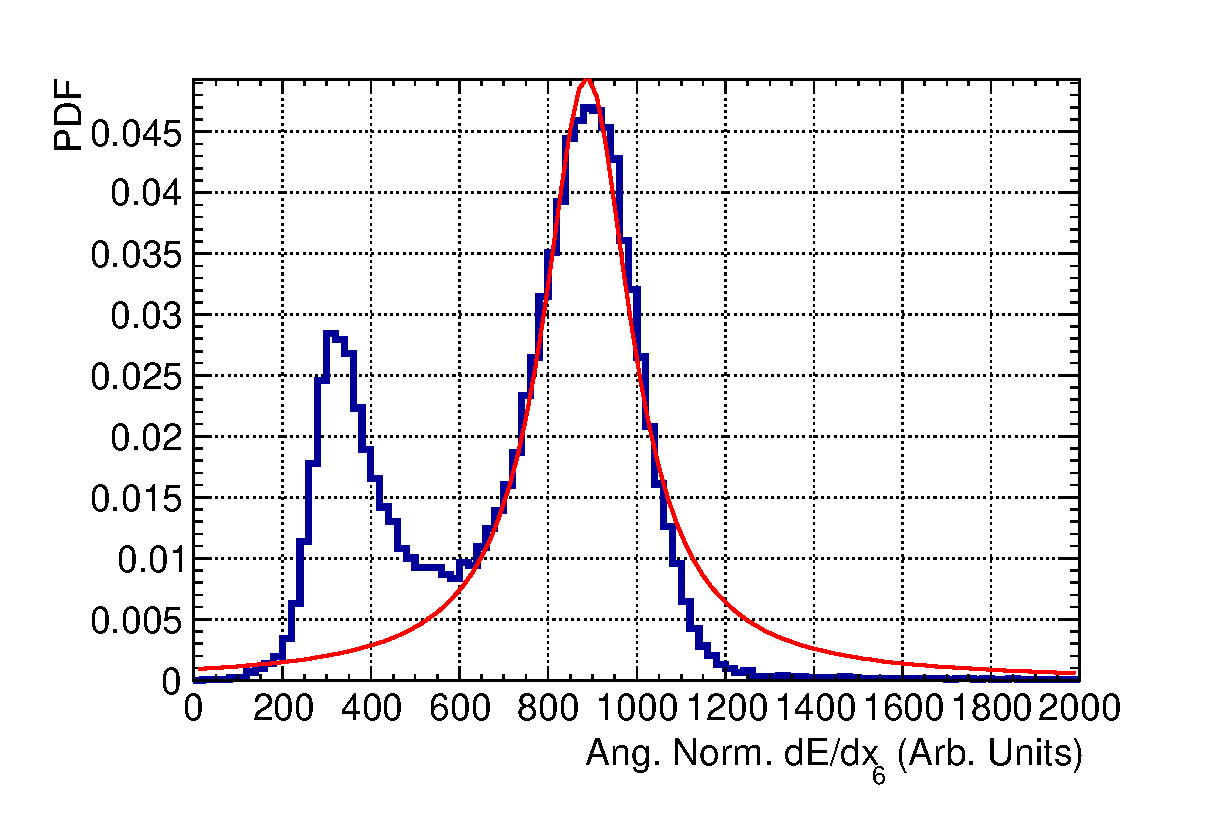
\includegraphics[width=\textwidth]{figures/sel/fig54f.eps}
         \caption{$\dedx_6$ Bragg peak value fit. The fitted peak value is $887.2$.}
         \label{subfig:dedx5-peak}
    \end{subfigure}
    \caption{Cauchy fits to extract the peak values of $\dedx$ at each node to estimate the average Bragg peak values. The corresponding fitted peak values are shown in each subfigure.}
    \label{fig:esc-andedx-peaks}
  \end{figure}

     The $\dedx$ for the last six nodes for each track can then be compared with this average profile using a $\chi^2$,
    \begin{equation}
    \chi^2 = \sum_{i=1}^{6} \frac{(\dedx_i - \overline{\dedx_i})^2}{\overline{\dedx_i}}
    \end{equation}
    A proton coming to rest should have a similar profile, so an upper cut on $\chi^2$ could further select protons with good momentum resolution. 
    Similar to the determination of the threshold for the individual $\dedx$, the momentum fractional difference is plotted against $\chi^2$, as shown in Fig.~\ref{fig:esc-mom-res-chi2}.
    \begin{figure}[ht]
       \centering
     %   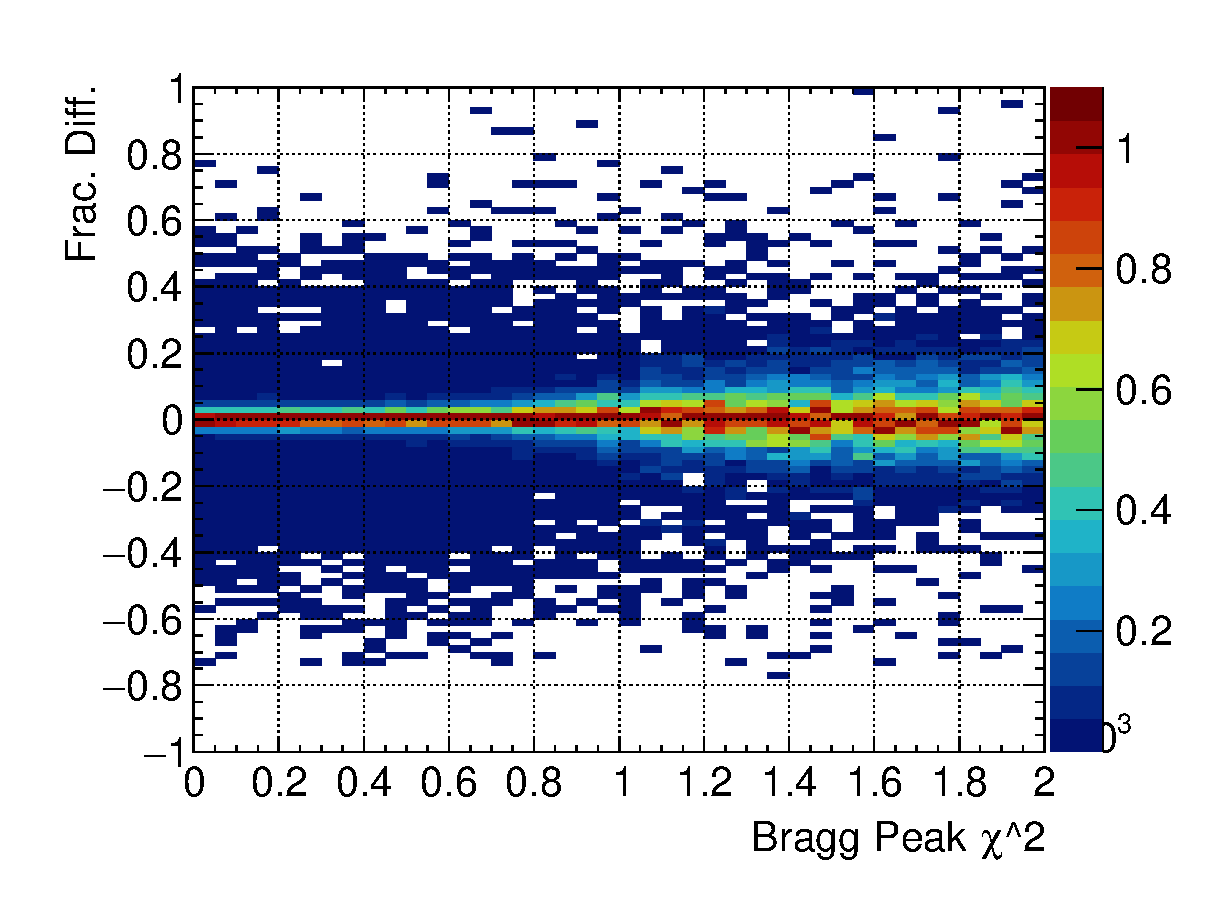
\includegraphics[width=\sgfidwid\textwidth]{figures/sel/brchi2_colnor_vs_p_pr_res_hist2d_al2_selpr_con_test.eps} 
       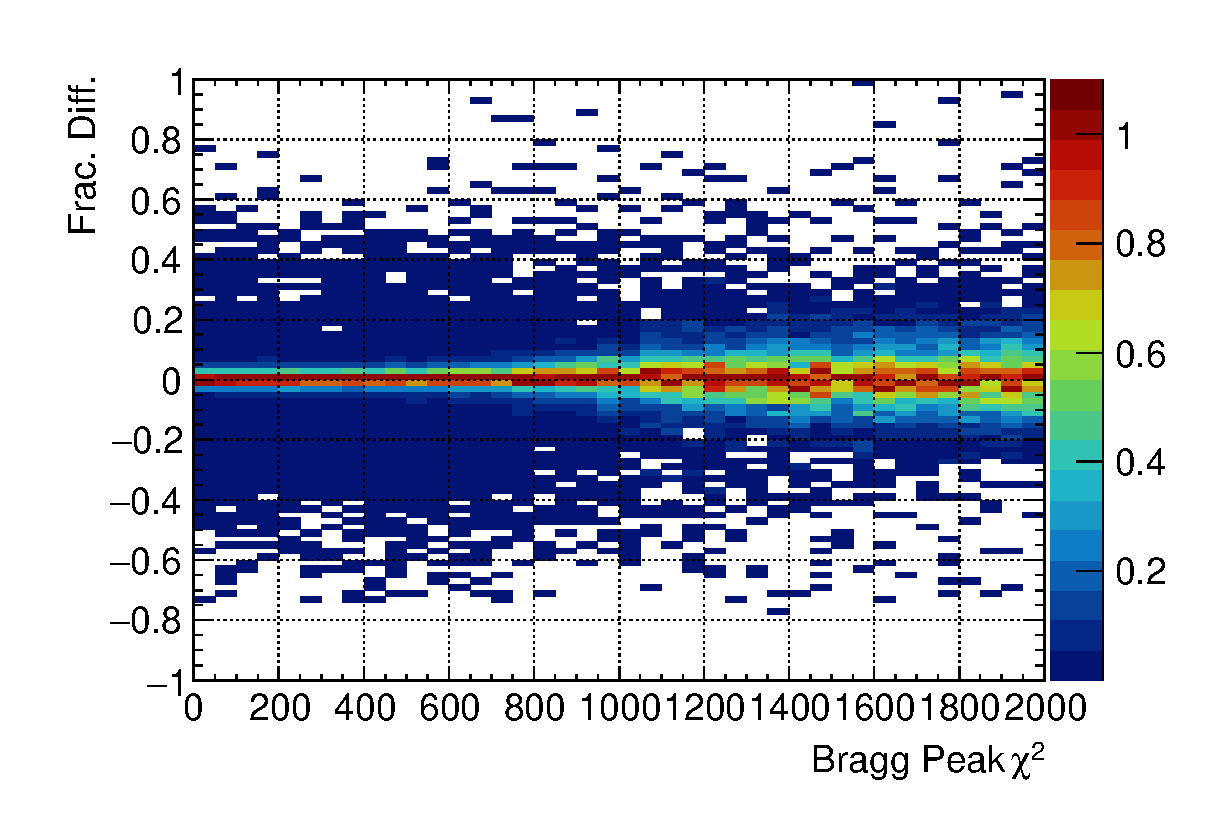
\includegraphics[width=\sgfidwid\textwidth]{figures/sel/fig55.eps} 
       \caption{Proton momentum reconstruction fractional difference against $\chi^2$ for determination of $\chi^2$ thresholds. Considerably larger fluctuations in reconstruction quality when $\chi^2$ is above $800$.}
       \label{fig:esc-mom-res-chi2}
    \end{figure}
    The upper cut on $\chi^2$ is implemented at $800$, above which considerably larger fluctuations are observed.

    \subsection{Momentum reconstruction bias assessment}
    \label{sec:sel-esc-bias}
     In Ref.~\cite{Lu:2016mjf}, reconstruction bias in the transverse component of the momentum is observed after the ESC implementation.
     Hence, such bias is also checked for the signal sample in SFGD.
     However, unlike in Ref.~\cite{Lu:2016mjf}, no apparent bias in proton momentum reconstruction is present, while such bias is observed in muon momentum reconstruction as shown in Fig.~\ref{fig:esc-prmupt}.

     \begin{figure}[ht]
     \centering
     \begin{subfigure}{\dbfigwid\textwidth}
          \centering
          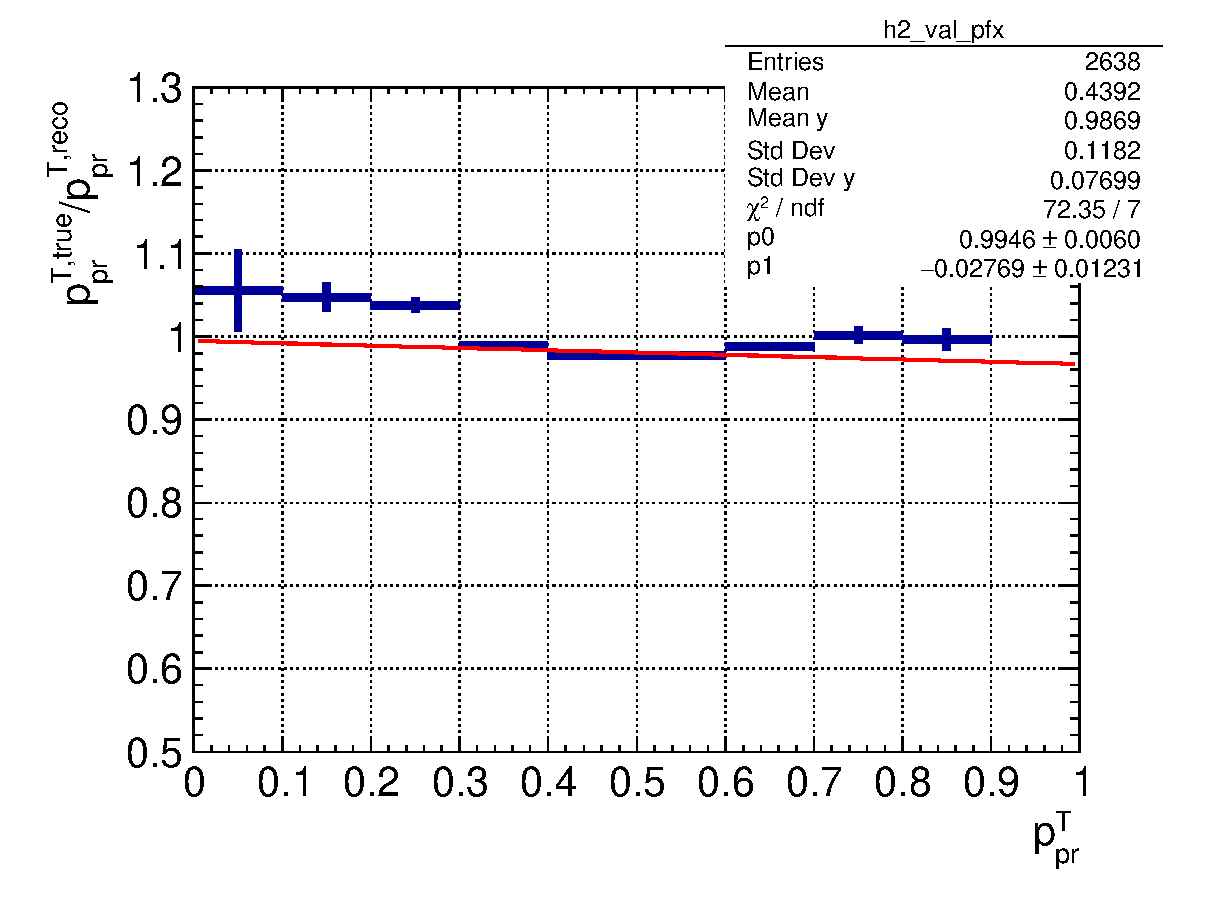
\includegraphics[width=\textwidth]{figures/sel/pr_pt_vs_pr_pt_bias_hist2d_al14.eps}
          \caption{Ratio of true$/$reco for proton $p_T$ against proton $\pt$.}
          \label{subfig:esc-prpt}
     \end{subfigure}
     \begin{subfigure}{\dbfigwid\textwidth}
          \centering
          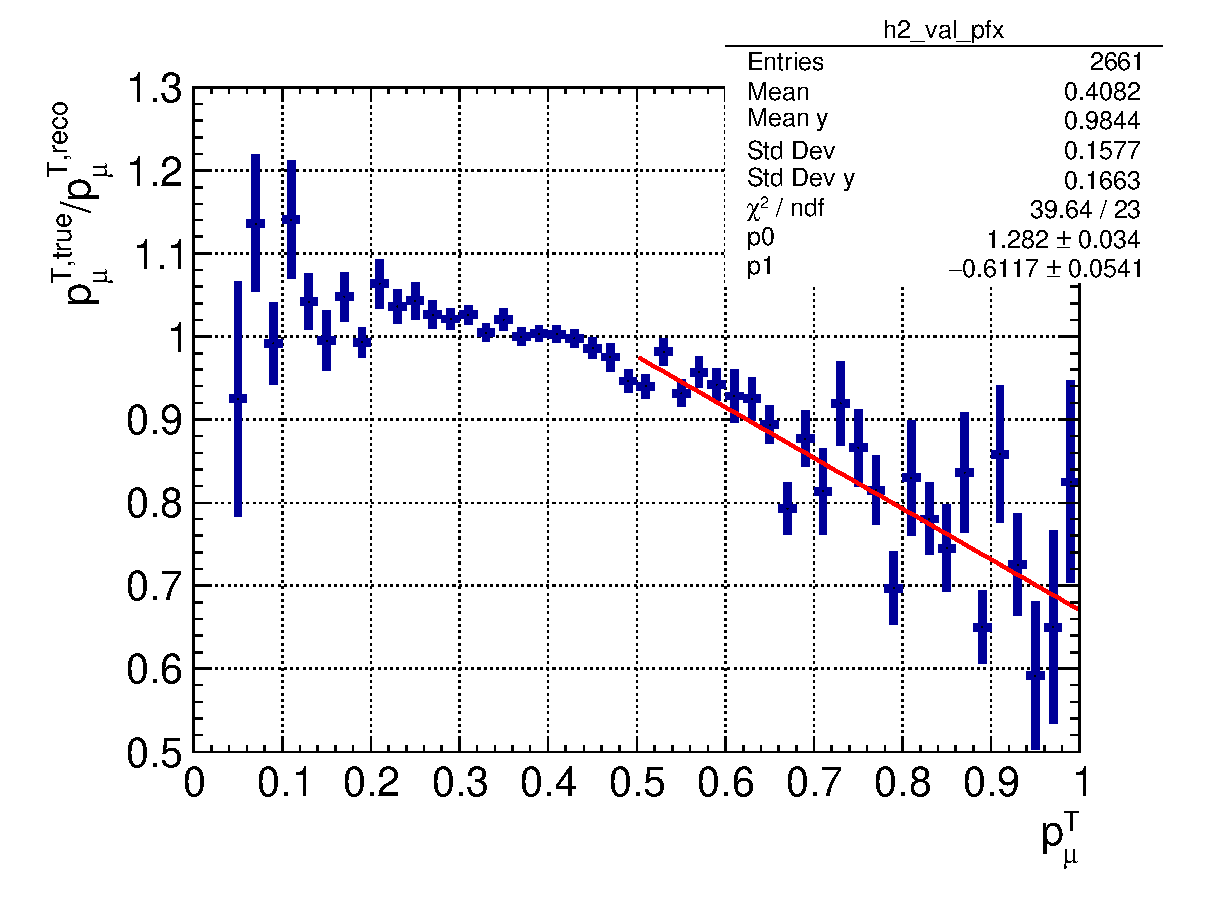
\includegraphics[width=\textwidth]{figures/sel/mu_pt_vs_mu_pt_bias_hist2d_al14.eps}
          \caption{Ratio of true$/$reco for muon $p_T$ against muon $\pt$.}
          \label{subfig:esc-mupt}
     \end{subfigure}
     \caption{Ratios of true$/$reco for the transverse component of the momentum for proton and muon are plotted against the transverse component for transverse momentum reconstruction bias assessment. No bias is observed for proton, while a linear bias is present for muon.}
     \label{fig:esc-prmupt}
     \end{figure}

     Further investigation shows that there is no bias in the muon angle, as shown in Fig.~\ref{subfig:esc-mutheta}.
     Additionally, such bias is shown to be present even before the implementation of the ESC step in Fig.~\ref{subfig:esc-mupt-bfesc}, while there is no appreciable bias in the full muon momentum reconstruction.
     This could be due to a bias in the neutrino direction reconstruction.
     However, such a direction bias should have affected the proton transverse momentum as well.
     As the impact is not pronounced and the simulation software is not the final stable version yet, a correction is done solely on the muon transverse momentum for the calculations of TKI variables, and further investigations on the root cause for this bias should be carried out after a stable simulation software version becomes available.

     \begin{figure}[ht]
     \centering
     \begin{subfigure}{\dbfigwid\textwidth}
          \centering
          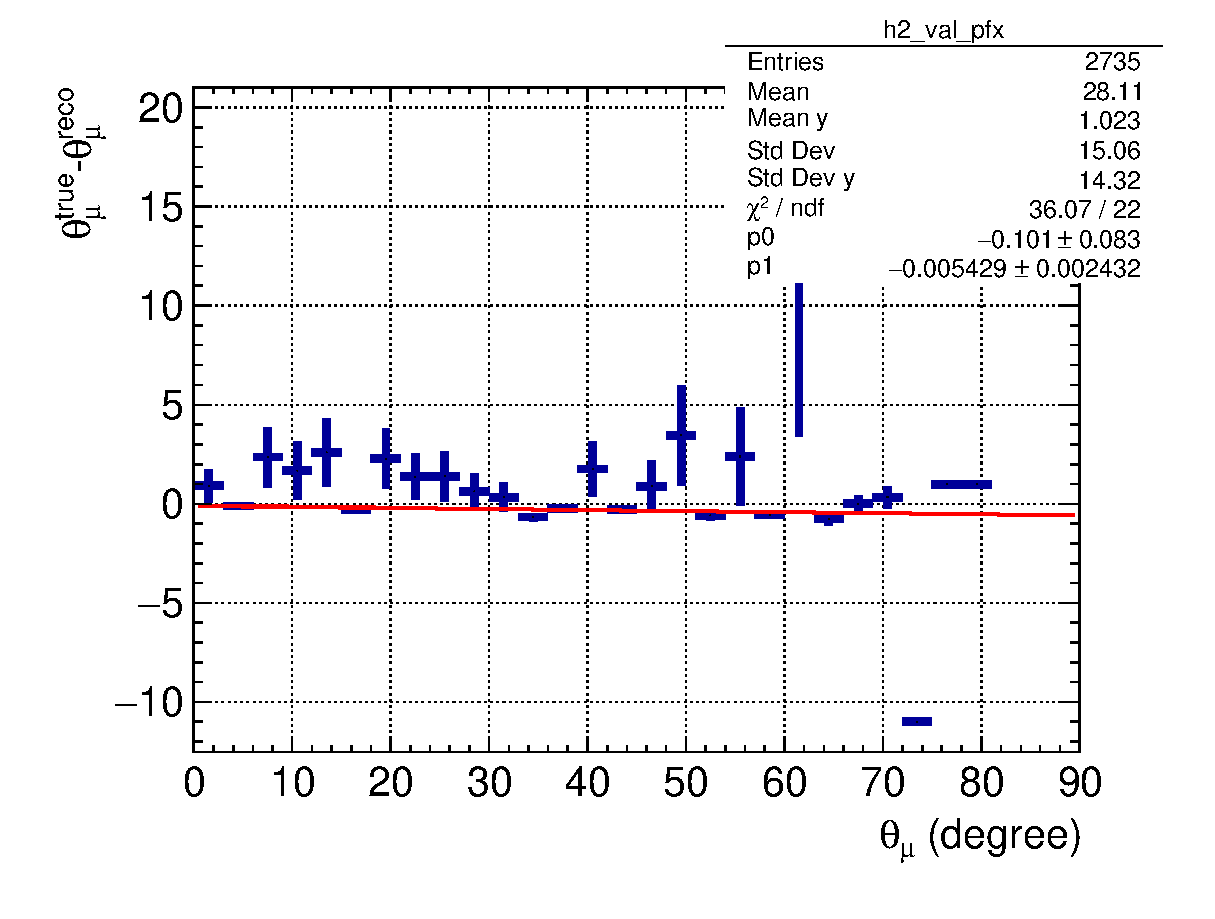
\includegraphics[width=\textwidth]{figures/sel/theta_mu_vs_theta_mu_res_hist2d_al14.eps}
          \caption{Value of true$-$reco for $\tmu$ against $\tmu$ before ESC selection.}
          \label{subfig:esc-mutheta}
     \end{subfigure}
     \begin{subfigure}{\dbfigwid\textwidth}
          \centering
          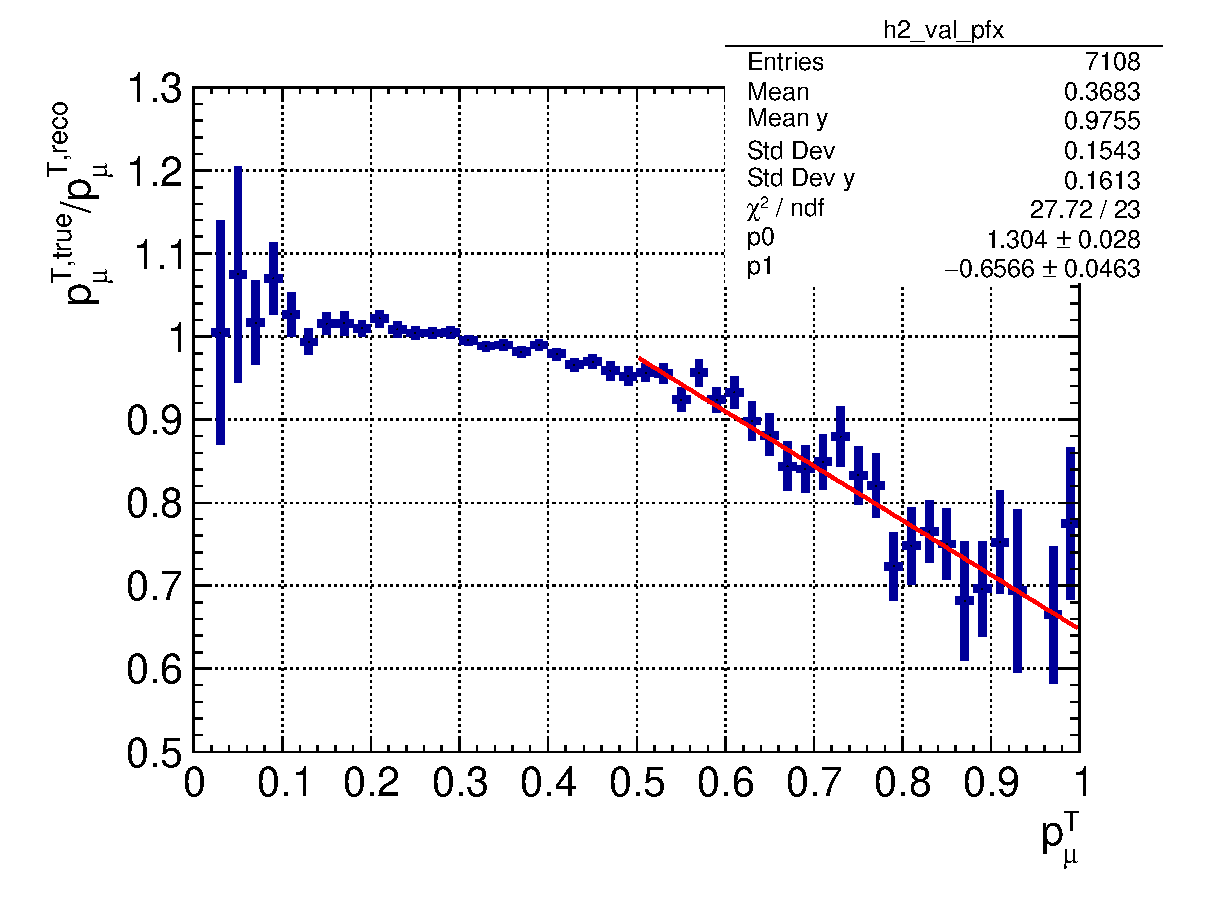
\includegraphics[width=\textwidth]{figures/sel/mu_pt_vs_mu_pt_bias_hist2d_al13.eps}
          \caption{Ratio of true$/$reco for muon $p_T$ against muon $\pt$ before ESC selection.}
          \label{subfig:esc-mupt-bfesc}
     \end{subfigure}
     \caption{Muon transverse momentum reconstruction bias investigation plots. There is bias in the muon angle reconstruction, while the transverse momentum bias is present even before the ESC selection.}
     \label{fig:esc-muptcor}
     \end{figure}

     The muon correction is applied through the inverse of the linear fit of the bias region between $0.5~\gevc$ and $1.1~\gevc$.
     The corrected muon transverse momentum is shown in Fig.~\ref{fig:esc-cormupt}, which demonstrates that the bias has been rectified.

     \begin{figure}[h]
     \centering
     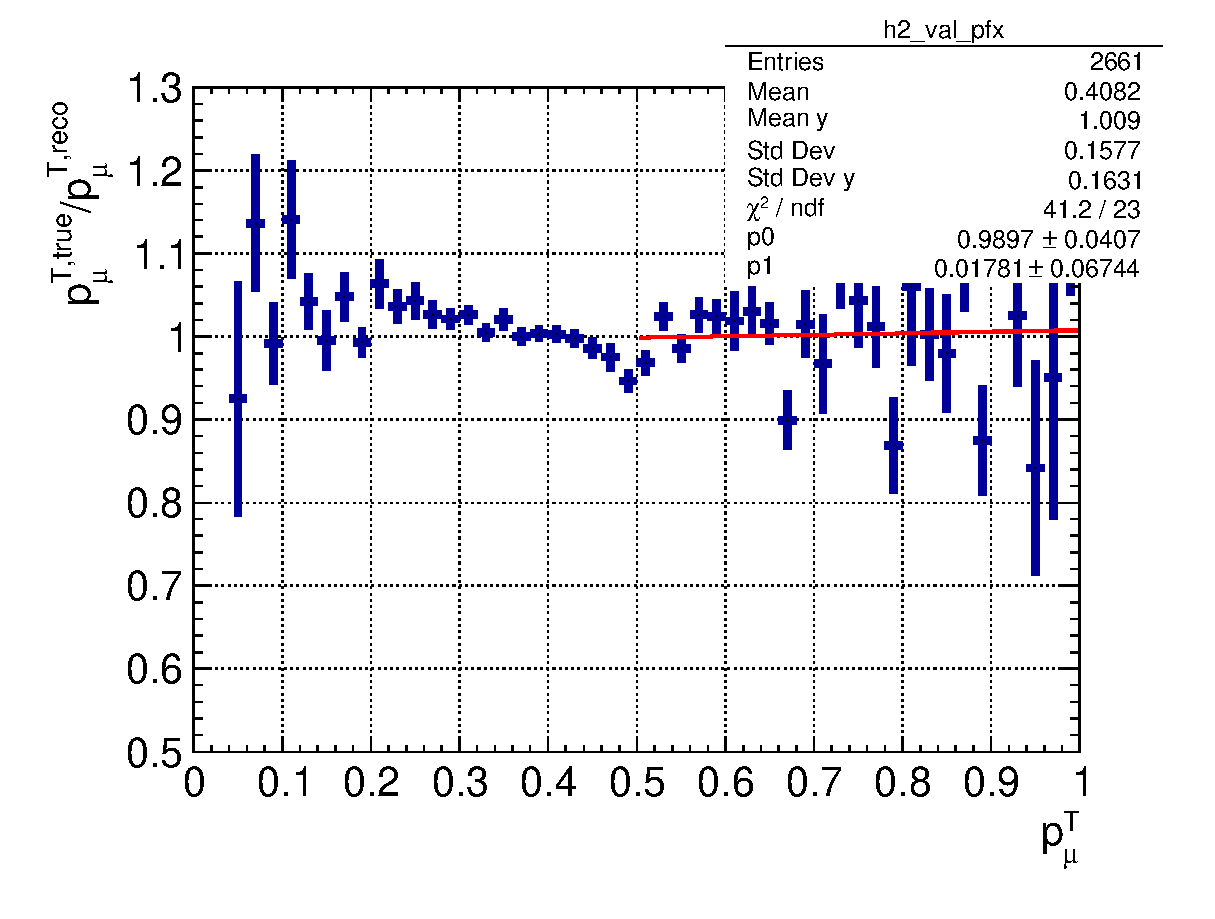
\includegraphics[width=\sgfidwid\textwidth]{figures/sel/mu_pt_vs_cor_mu_pt_bias_hist2d_al14.eps} 
     \caption{Ratio of true$/$reco for muon $p_T$ against muon $\pt$ after correction. The nearly flat line suggests that the bias has been rectified.}
     \label{fig:esc-cormupt}
     \end{figure}

    \subsection{Impacts on Single Particle Kinematics}
     The ESC technique is completed with the transverse momentum bias correction.
     The overall impact of the technique on the reconstructed single particle kinematics (SPK), i.e. reconstructed proton kinematics in this case, is shown in Fig.~\ref{fig:esc-spk}.
     It has significantly reduced off-diagonal entries, which represent badly reconstructed events.
     Moreover, the conspicuous line with a negative slope in the $\tpr$ has mostly disappeared.
     These could be due to a mis-reconstruction of the track direction for short protons, which are excluded by the first requirement of the ESC step: the number of nodes has to be at least $6$.
     
     \begin{figure}[ht]
        \centering
        \begin{subfigure}{\dbfigwid\textwidth}
             \centering
             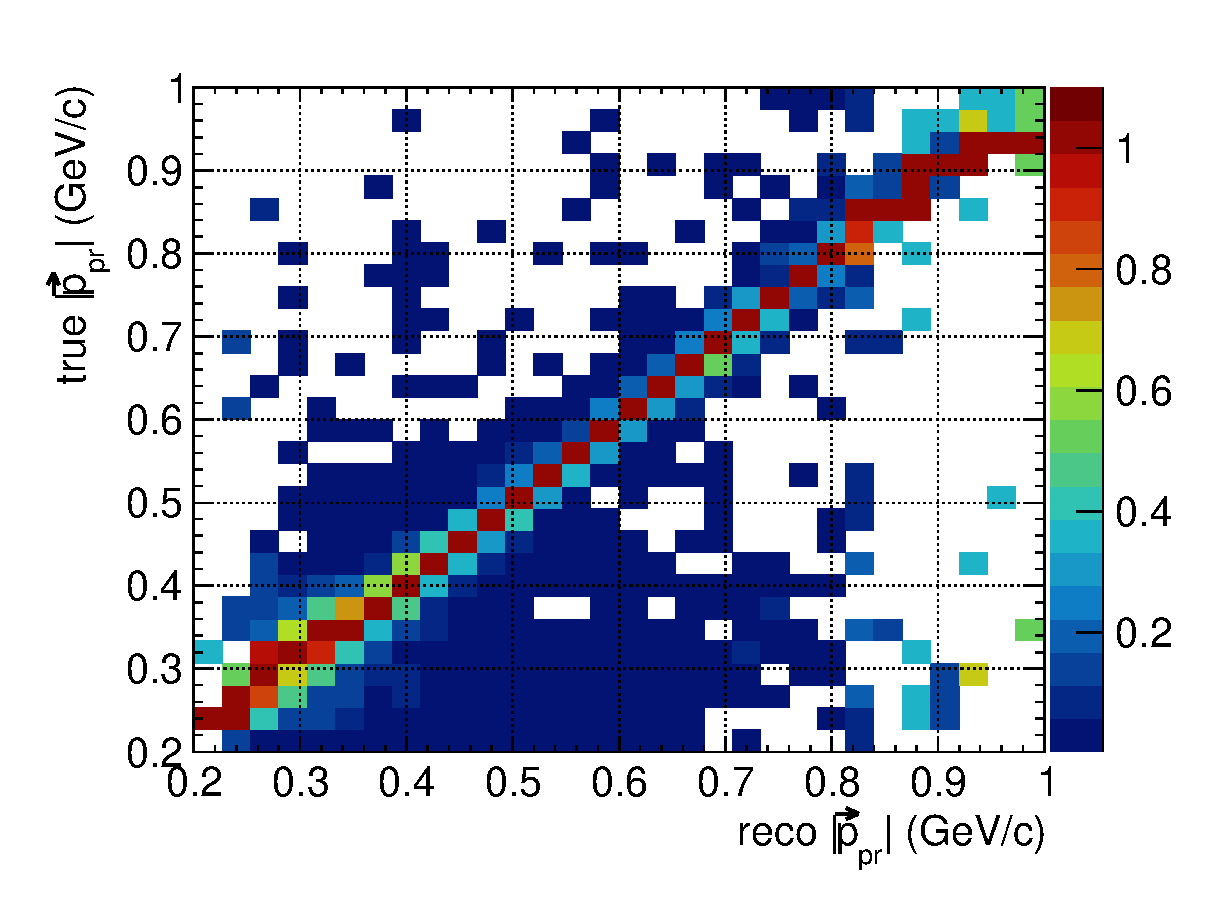
\includegraphics[width=\textwidth]{figures/sel/p_pr_colnor_resmat_al13.eps}
             \caption{$\ppr$ before ESC selection.}
             \label{subfig:esc-ppr-bfesc}
        \end{subfigure}
        \begin{subfigure}{\dbfigwid\textwidth}
             \centering
             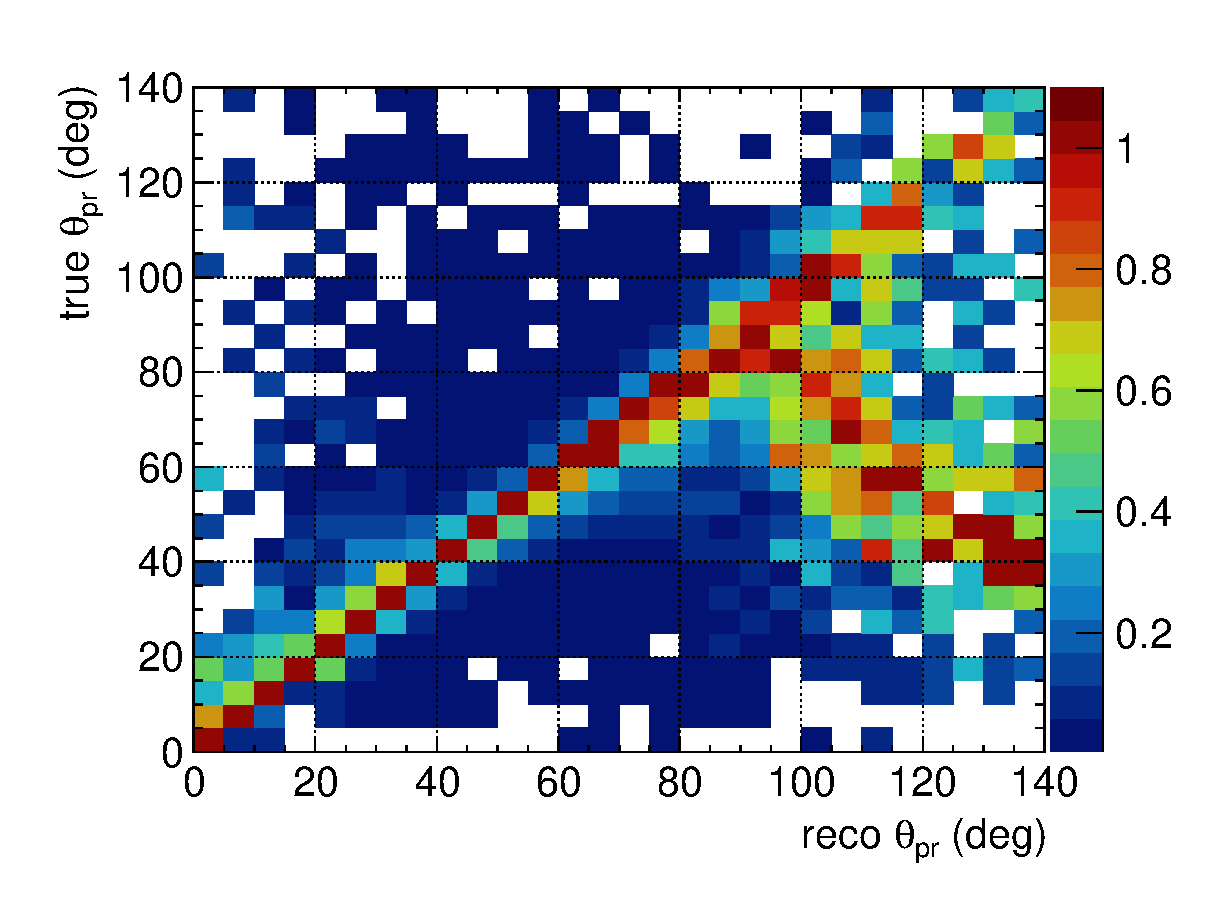
\includegraphics[width=\textwidth]{figures/sel/theta_pr_colnor_resmat_al13.eps}
             \caption{$\tpr$ before ESC selection.}
             \label{subfig:esc-tpr-bfesc}
        \end{subfigure}
        \\
        \begin{subfigure}{\dbfigwid\textwidth}
             \centering
             \includegraphics[width=\textwidth]{figures/sel/p_pr_colnor_resmat_al14.eps}
             \caption{$\ppr$ after ESC selection.}
             \label{subfig:esc-ppr-afesc}
        \end{subfigure}
        \begin{subfigure}{\dbfigwid\textwidth}
             \centering
             \includegraphics[width=\textwidth]{figures/sel/theta_pr_colnor_resmat_al14.eps}
             \caption{$\tpr$ after ESC selection.}
             \label{subfig:esc-tpr-afesc}
        \end{subfigure}
        \caption{Reconstruction quality plots of truth against reconstruction values for SPK variables before (top) and after (bottom) selection. A significant reduction in the off-diagonal entries for both $\ppr$ and $tpi$ is observed after the ESC selection, indicating a better reconstruction quality. The conspicuous line with a negative slope for $\tpr$ has mostly disappeared.}
        \label{fig:esc-spk}
  \end{figure}

     The overall improvement in the SPK is best illustrated with a Cauchy fit to the proton momentum reconstruction resolution histogram, as shown in Fig.~\ref{subfig:ppr-res-bfESC} and Fig.~\ref{subfig:ppr-res-afESC}, which shows a more than $50\%$ reduction in the fitted half width at half maximum (HWHM) of the distribution.
     This improvement is achieved at the cost of a two-thirds reduction in efficiency, as shown in Fig.~\ref{subfig:ppr-eff-bfESC} and Fig.~\ref{subfig:ppr-eff-afESC}.
     The drop in efficiency might seem drastic, but it proves to be necessary for the TKI analysis, as shown later in Sec.~\ref{sec:mc-tki}, which showcases the significant improvement in the evaluation of TKI variables due to the ESC technique.

   \begin{figure}[t]
      \centering
      \begin{subfigure}{\dbfigwid\textwidth}
           \includegraphics[width=\textwidth]{figures/sel/p_pr_res_pdf_al13_zoom.eps}
           \caption{$\pp$ resolution before ESC selection. The fitted HWHM is about $3.5\%$.}
           \label{subfig:ppr-res-bfESC}
      \end{subfigure}
      \begin{subfigure}{\dbfigwid\textwidth}
           \includegraphics[width=\textwidth]{figures/sel/p_pr_eff_al13.png}
           \caption{Selection efficiency before ESC selection. The overall efficiency is $2113/8182\approx25.8\%$.}
           \label{subfig:ppr-eff-bfESC}
      \end{subfigure}
      \\
      \begin{subfigure}{\dbfigwid\textwidth}
           \includegraphics[width=\textwidth]{figures/sel/p_pr_res_pdf_al14_zoom.eps}
           \caption{$\ppr$ resolution after ESC selection. The fitted half width is about $1.6\%$.}
           \label{subfig:ppr-res-afESC}
      \end{subfigure}
      \begin{subfigure}{\dbfigwid\textwidth}
           \includegraphics[width=\textwidth]{figures/sel/p_pr_eff_al14.png}
           \caption{Selection efficiency after ESC selection. The overall efficiency is $736/8182\approx9.0\%$}
           \label{subfig:ppr-eff-afESC}
      \end{subfigure}
      \caption{Proton ESC selection results. The grey histograms are the true probability distribution, while the pink ones are those that get reconstructed. The selection efficiency has dropped from $25.8\%$ to $9.0\%$, while the proton momentum reconstruction resolution has improved from a fitted HWHM of $3.5\%$ to $1.6\%$.}
      \label{fig:esc-ppr-reseff}
   \end{figure}


    %------------------- pion TL ----------------%
    \section{Pion Trackless Reconstruction}
       \label{sec:sel-tl}
          As briefly elaborated in Sec.~\ref{sec:t2k-sw}, in SFGD, particle identification and momentum reconstruction are only performed on reconstructed tracks, which have a minimum length of about $30$~mm. 
          Hence, low-momentum particles, which travel only a short distance, could not be reconstructed at all. 
          When these low-momentum pions are not reconstructed, these $\ccopi$ events are misidentified as $\cczpi$ events, both decreasing the signal for the $\ccopi$ samples and increasing the background for the $\cczpi$ sample. 
          Thus, it would be highly beneficial if we could reconstruct these pions. 
          The pion trackless reconstruction technique I have developed can address this gap well.

          \subsection{Working Principles}
          \label{sec:tl-wp}
          The trackless technique is an advancement of previous methods. 
          It was first attempted in MINER$\nu$A~\cite{poster:minerva-pime} and in the Fine Grain Detectors of ND280~\cite{poster:minerva-pime}. 
          In MINER$\nu$A, a reconstructed cluster must be identified as a pion candidate. 
          In contrast, ND280 includes a prototype of the trackless reconstruction; however, it is integrated with other pion reconstruction methods, and its full potential has not yet been explored.

          This reconstruction technique is based on two key aspects of the pion decay chain, $\pi \rightarrow \mu \rightarrow e$:

          \begin{enumerate}
          \item \textbf{Delayed Michel Electron (ME) Signal:} The ME, as the grandchild in the decay chain, produces a delayed signal that occurs on a much longer timescale compared to other processes, such as $\piz$ decay. 
          Consequently, the presence of the primary pion can be inferred from the delayed ME signal in the SFGD.
          
          \item \textbf{Kinematic Determination via Energy-Momentum Conservation:} The pion decay, $\pi \rightarrow \mu + \nu$, is a two-body process. 
          The kinematics of the daughter particles are entirely determined by energy-momentum conservation. 
          When a pion decays at rest, the daughter muon moves only about $0.12~\textrm{cm}$. 
          Therefore, the starting point of the ME provides a reliable estimate of the pion's endpoint.
          \end{enumerate}

          Using the distance between the primary neutrino interaction vertex and the ME starting point, the pion momentum can be reconstructed by range. 
          Note that the pion must decay at rest for this technique to be applicable. 
          For pions that undergo secondary interactions, their range does not correlate with their momentum, so their momentum cannot be reconstructed by range.
          For a pion decaying in flight, its daughter muon will have a non-negligible momentum and hence travel an appreciable distance before decaying into the ME.
          Hence, the ME starting point is no longer a good estimate of the pion's endpoint.
          Alternatively, the muon starting point can be used to estimate the pion's  endpoint, but the range of the pion does not correlate with the pion starting momentum well as the ending momentum is non-zero.
          It might be possible to reconstruct the pion's ending momentum from the muon momentum due to the two-body decay kinematics, and then to reconstruct the pion's starting momentum from the pion's range and its ending momentum.
          This will be an interesting avenue to explore in the future, while the current analysis focuses on pions decaying at rest.

          For these target pions, an empirical relationship between the pion's kinetic energy and its range was established using a PGUN sample, as shown in Fig.~\ref{fig:pi-mombr-fit}. 
          The PGUN sample initiates pions from the centre of SFGD and propagates them isotropically. 
          It comprises $500,000$ events with kinetic energies uniformly distributed between $20~\mev$ and $200~\mev$. 
          The $\log_{10}$ of the true kinetic energy is plotted against the true pion length in Fig.~\ref{fig:pi-mombr-fit}.
          The central region of the plots is fitted with a fourth-order polynomial.
          Although the $\chindf$ of the fit is relatively large, the fitted line matches the data points well.
          Since the simulation is not yet final, this fit is sufficient for the current analysis and should be updated once the simulation is finalized.
          \begin{figure}[ht]
          \centering
          \includegraphics[width=\sgfidwid\textwidth]{figures/sel/pi_len_pi_len_vs_pi_ke_hist2d_al0_true_nokink.eps} 
          \caption{A degree 4 polynomial fit of $\log_{10}{T_\pi}$ against $\log_{10}{L_\pi}$, where $T_\pi$ and $L_\pi$ are the kinetic energy and the range of the pion, respectively. The $p_i$'s are the corresponding coefficients of the term of order $i$. The fit matches the data points well.}
          \label{fig:pi-mombr-fit}
          \end{figure}

       \subsection{Preliminary Study on Pion Fates}
       \label{sec:tl-ps}
          Before implementing the pion trackless reconstruction technique, it is essential to assess its potential significance, as this technique can only reconstruct pions that decay at rest. 
          If only a limited number of pions decay in this manner, the technique would be inapplicable. 
          Therefore, a preliminary study on pion fates relevant to T2K was conducted.

          The first step involved examining the primary pion momentum distribution in SFGD as produced by the T2K neutrino beam. 
          For a rough estimation, the first 100,000 events in the T2K input flux file were processed through the T2K ND simulation, and events containing a primary pion were recorded. 
          The true pion momentum cumulative distribution is shown in Fig.~\ref{subfig:pi-mom-cum}, indicating that the majority of pions have momentum below $1000~\mevc$.

          \begin{figure}[t]
               \centering
               \begin{subfigure}{\dbfigwid\textwidth}
                    \includegraphics[width=\textwidth]{figures/sel/pion_mom_pdf.png}
                    \caption{Primary pion momentum cumulative distribution. The median momentum is about $300~\mevc$.}
                    \label{subfig:pi-mom-cum}
               \end{subfigure}
               \begin{subfigure}{\dbfigwid\textwidth}
                    \includegraphics[width=\textwidth]{figures/sel/pion_theta_pdf.png}
                    \caption{Primary pion angle cumulative distribution. The $80\%$ angle is $87^\circ$.}
                    \label{subfig:pi-theta-cum}
               \end{subfigure}
               \caption{Cumulative density functions of primary pion kinematics in SFGD. The relevant values are extracted for subsequent investigation of pion fates.}
          \end{figure}
               
          The median momentum is approximately $300~\mevc$, with about $30\%$ of pions having momentum below $200~\mevc$ and $80\%$ below $800~\mevc$. 
          Similarly, the pion angle distribution, depicted in Fig.~\ref{subfig:pi-theta-cum}, shows that approximately $80\%$ of pions have an angle below $87^\circ$.

          The second step is to simulate pion propagation in SFGD with the relevant kinematics. 
          A total of six samples, each containing 10,000 events, were simulated with pions traveling at momenta of $200~\mevc$, $300~\mevc$, and $800~\mevc$, and angles of $0^\circ$ and $70^\circ$. 
          Since SFGD reconstruction is largely independent of pion direction, the $70^\circ$ samples serve as consistency checks. 
          For each sample, the fate of each pion was determined using the truth information.

          A total of ten fate topologies are defined as follows:
          \begin{enumerate}
          \item \textbf{DK@rest (Good)} – The pion decays at rest, and the total number of true trajectories is three, corresponding to $\pip$, $\mu$, and the ME exactly. 
          This represents a clean pion decay-at-rest event.
          \item \textbf{DK@rest (Dirty)} – Similar to the previous fate, but the total number of true trajectories exceeds three. 
          The additional trajectories are mostly electromagnetic showers due to the ME.
          \item \textbf{DK@flight} – The pion decays with non-zero momentum, resulting in a relatively large starting momentum for the daughter muon.
          \item \textbf{Elastic Knock-out} – The pion undergoes secondary interactions (SI), leading to the liberation of an additional proton. 
          The pion continues to propagate and decay, but its range is no longer well correlated with its starting momentum.
          \item \textbf{Deflection} – The pion undergoes SI. 
          No additional particles are produced, but its direction changes.
          \item \textbf{Absorption} – Another type of SI where the pion does not emerge from its interaction with the nucleus, so no ME is present.
          \item \textbf{Charge Exchange} – The $\pip$ is converted to a $\piz$ via a charge exchange interaction with the nucleus. 
          Since $\piz$ decays much faster, no ME is present.
          \item \textbf{$\pim$} – While there is no single interaction that can convert a $\pip$ to a $\pim$, this fate—where a $\pim$ appears as one of the daughters of the $\pip$—is observed, albeit rarely, due to complex pion SI within the nucleus.
          \item \textbf{Escaped} – The pion escapes SFGD before decaying. 
          Regardless of its subsequent decay, the potential ME cannot be detected in SFGD.
          \item \textbf{Others} – This category includes all uncategorised events, such as cases where the pion produces delta ray electrons or undergoes bremsstrahlung. 
          These events are relatively rare and do not require special treatment.
          \end{enumerate}

          Fates 1 through 3 involve pions that decay before any secondary interactions, i.e., pions decay via the chain $\pi \rightarrow \mu \rightarrow e$. 
          Thus, these pions can be tagged by the presence of the ME. 
          However, as illustrated in Sec.~\ref{sec:tl-wp}, the trackless technique relies on the extremely short distance travelled by the daughter muon. 
          Pions decaying in flight result in a longer distance travelled by the daughter muon, making them unsuitable for the trackless technique.

          Fates 4 through 8 involve pions that undergo secondary interactions, resulting in the absence of the ME, except for those that experience deflection, which also renders them unsuitable for the trackless technique. 
          The range of a deflected pion does not correlate well with its momentum, further disqualifying it from being reconstructed by the trackless technique. 
          In summary, the trackless technique is most applicable to Fates 1 and 2.

          The fate distributions are shown in Fig.~\ref{fig:pi-fate}. 
          For the $200~\mevc$ samples, both at $0^\circ$ and $70^\circ$, more than $70\%$ of the pions fall into Fates 1 and 2. 
          In the $300~\mevc$ samples, this fraction drops to $30\%$ for the $0^\circ$ angle and about $12\%$ for the $70^\circ$ angle. 
          This trend is expected because as pion momentum increases, the decay length increases, and the probability of secondary interactions rises. 
          The further decrease observed at $70^\circ$ is attributed to an increased escape fraction. 
          The geometry of SFGD, being much shorter in the vertical direction, facilitates the escape of high-angle pions. 
          For $800~\mevc$ pions, the decay length is too long for SFGD, resulting in a significant increase in the escape fraction—approximately $30\%$ at $0^\circ$ and $50\%$ at $70^\circ$. 
          The unescaped pions are those that have undergone secondary interactions, rendering them not reconstructable by the trackless technique at this high momentum.
          \begin{figure}[ht]
               \centering
               \begin{subfigure}{\dbfigwid\textwidth}
                    \includegraphics[width=\textwidth]{figures/sel/pion_fate_200_0.png}
                    \caption{$\ppi=200\mevc$ and $\tpi=0^\circ$.}
                    \label{subfig:pi-fate-200-0}
               \end{subfigure}
               \begin{subfigure}{\dbfigwid\textwidth}
                    \includegraphics[width=\textwidth]{figures/sel/pion_fate_200_70.png}
                    \caption{$\ppi=200\mevc$ and $\tpi=70^\circ$.}
                    \label{subfig:pi-fate-200-70}
               \end{subfigure}
              \\
               \begin{subfigure}{\dbfigwid\textwidth}
                    \includegraphics[width=\textwidth]{figures/sel/pion_fate_300_0.png}
                    \caption{$\ppi=300\mevc$ and $\tpi=0^\circ$.}
                    \label{subfig:pi-fate-300-0}
               \end{subfigure}
               \begin{subfigure}{\dbfigwid\textwidth}
                    \includegraphics[width=\textwidth]{figures/sel/pion_fate_300_70.png}
                    \caption{$\ppi=300\mevc$ and $\tpi=70^\circ$.}
                    \label{subfig:pi-fate-300-70}
               \end{subfigure}
              \\
               \begin{subfigure}{\dbfigwid\textwidth}
                    \includegraphics[width=\textwidth]{figures/sel/pion_fate_800_0.png}
                    \caption{$\ppi=800\mevc$ and $\tpi=0^\circ$.}
                    \label{subfig:pi-fate-800-0}
               \end{subfigure}
               \begin{subfigure}{\dbfigwid\textwidth}
                    \includegraphics[width=\textwidth]{figures/sel/pion_fate_800_70.png}
                    \caption{$\ppi=800\mevc$ and $\tpi=70^\circ$.}
                    \label{subfig:pi-fate-800-70}
               \end{subfigure}
               \caption{Pion fates in the SFGD for different combinations of pion kinematics. A significant fraction, approximately $80\%$ of pion decays at rest at $\ppi=200\mevc$ regardless of the angle. The fraction drops to about $30\%$ at $\ppi=300\mevc$ for low angles and $10\%$ for high angles, and further decreases to $0\%$ at $\ppi=800\mevc$.}
               \label{fig:pi-fate}
            \end{figure}
       
          This preliminary study demonstrates that a considerable fraction of the primary pions produced in SFGD have relatively low momentum ($<200~\mevc$). 
          For these pions, the majority decay at rest, producing an ME that can be utilized in the trackless technique. 
          Thus, the trackless technique is applicable to approximately $30\%$ of the total pion events in SFGD, making it a significant reconstruction method to develop.


     \subsection{Implementation}
     \label{sec:tl-imp}
          The pion trackless reconstruction is integrated into my $\numuccopi$ selection, which builds upon the existing $\numucc$-inclusive selection. 
          Therefore, it is appropriate to discuss the trackless technique within the context of the $\numuccopi$ selection.

          The $\numucc$-inclusive selection identifies the primary vertex position and the primary muon, providing the trackless reconstruction with a reliable approximation of the pion's starting point. 
          The following steps are implemented to identify suitable ME candidates and reconstruct the pion momentum in the $\numuccopi$ selection:
          \begin{itemize}
          \item \textbf{Step 0 - $\numucc$-inclusive Selection}
          \item \textbf{Step 1 - Find Suitable ME Candidates}
          \item \textbf{Step 2 - One Trackless Pion Cut}
          \item \textbf{Step 3 - Kink Cut}
          \item \textbf{Step 4 - Background Reduction}
          \end{itemize}
          \textbf{Find Suitable ME Candidates} – Iterate through all delayed reconstructed objects with more than one hit. 
          If an object occurs $30.0~\textrm{ns}$ after the primary vertex time, it is saved as a potential ME candidate. 
          However, ME candidates may trigger showers, resulting in additional delayed reconstructed objects. 
          To distinguish the true ME from these secondary objects, the "prompt energy" technique used by MINERvA~\cite{Zhang:2016glf} is employed. 
          Prompt energy refers to the energy deposited by the short muon and pion. 
          Although these particles may have insufficient energy to form a reconstructable track, they still deposit energy much earlier than the ME onset. 
          Therefore, by examining the energy deposition within $30~\textrm{mm}$ around both ends of an ME candidate, it can be determined if energy was deposited $30~\textrm{ns}$ prior, confirming the suitability of the ME candidate. 
          Additionally, if the primary muon is contained within SFGD, it may also decay and produce an indistinguishable ME based solely on time delay. 
          To address this, an additional check excludes ME candidates near the end of the identified primary muon.

          \textbf{One Trackless Pion Cut} – Select events that have exactly one proper ME candidate.

          \textbf{Kink Cut} – Since the trackless reconstruction does not require the ME to be adjacent to a primary track, it cannot differentiate pions travelling directly from the primary interaction to decay at rest from those that have been deflected before decaying at rest. 
          To ensure accurate momentum-by-range reconstruction, events with deflected pions are rejected. 
          Specifically, any event with an ME connected to non-primary tracks is excluded.

          \textbf{Background Reduction} – Multiple background reduction steps are implemented, including an existing $\pi^0$ rejection developed by colleagues at T2K. 
          However, these measures are insufficient, as evidenced by the significant portion of CC-other backgrounds in Figs.~\ref{subfig:tlpi-ppi-bf-trknumcut-tpc}, \ref{subfig:tlpi-tpi-bf-trknumcut-tpc}, \ref{subfig:tlpi-ppi-bf-trknumcut-sfg}, and \ref{subfig:tlpi-tpi-bf-trknumcut-sfg}. 
          Therefore, based on a logical understanding of different event topologies, I developed a series of track number cuts and introduced a new concept called the "track family tree."

          An event topology resembles a family tree sideways. 
          The first generation consists of the primary tracks, while the second generation includes tracks connected to the ends of the primary tracks. 
          The family tree tracing step involves looping through all reconstructed tracks to build the family tree starting from the primary vertex. 
          One useful variable is the number of generations. 
          A $\numuccopi$ event should not have a large number of generations, as the primary pion can have an ME attached to its end without producing showers or multiple scatterings. 
          Therefore, the number of generations is required to be fewer than three. 
          Another associated variable is the number of lone tracks, which are not connected to any tracks in the family tree. 
          A clean $\numuccopi$ event should have a limited number of lone tracks, which could result from noise or low-energy scattering of the ME, leading to clusters isolated from the ME track. 
          Further details on the other track number cuts are provided in Appendix.~\ref{sec:app-tlpi-trknumcut}. 
          The overall impact of the track number cuts is illustrated by the topological decomposition of the pion kinematic distributions in Fig.~\ref{fig:tl-trknum-cut-res}.
          \begin{figure}
             \centering
             \begin{subfigure}[!htb]{\dbfigwid\textwidth}
                  \includegraphics[width=\textwidth]{figures/sel/TPCmu_p_pi_stack_al8.eps}
                  \caption{TPC-$\mu$: $\ppi$ before track number cut.}
                  \label{subfig:tlpi-ppi-bf-trknumcut-tpc}
             \end{subfigure}
             \begin{subfigure}[!htb]{\dbfigwid\textwidth}
                  \includegraphics[width=\textwidth]{figures/sel/TPCmu_p_pi_stack_al9.eps}
                  \caption{TPC-$\mu$: $\ppi$ after track number cut.}
                  \label{subfig:tlpi-ppi-af-trknumcut-tpc}
             \end{subfigure}
             \\
             \begin{subfigure}[!htb]{\dbfigwid\textwidth}
                  \includegraphics[width=\textwidth]{figures/sel/TPCmu_theta_pi_stack_al8.eps}
                  \caption{TPC-$\mu$: $\tpi$ before track number cut.}
                  \label{subfig:tlpi-tpi-bf-trknumcut-tpc}
             \end{subfigure}
             \begin{subfigure}[!htb]{\dbfigwid\textwidth}
                  \includegraphics[width=\textwidth]{figures/sel/TPCmu_theta_pi_stack_al9.eps}
                  \caption{TPC-$\mu$: $\tpi$ after track number cut.}
                  \label{subfig:tlpi-tpi-af-trknumcut-tpc}
             \end{subfigure}
             \\
             \begin{subfigure}[!htb]{\dbfigwid\textwidth}
                  \includegraphics[width=\textwidth]{figures/sel/SFGmu_p_pi_stack_al8.eps}
                  \caption{SFGD-$\mu$: $\ppi$ before track number cut.}
                  \label{subfig:tlpi-ppi-bf-trknumcut-sfg}
             \end{subfigure}
             \begin{subfigure}[!htb]{\dbfigwid\textwidth}
                  \includegraphics[width=\textwidth]{figures/sel/SFGmu_p_pi_stack_al9.eps}
                  \caption{SFGD-$\mu$: $\ppi$ after track number cut.}
                  \label{subfig:tlpi-ppi-af-trknumcut-sfg}
             \end{subfigure}
             \\
             \begin{subfigure}[!htb]{\dbfigwid\textwidth}
                  \includegraphics[width=\textwidth]{figures/sel/SFGmu_theta_pi_stack_al8.eps}
                  \caption{SFGD-$\mu$: $\tpi$ before track number cut.}
                  \label{subfig:tlpi-tpi-bf-trknumcut-sfg}
             \end{subfigure}
             \begin{subfigure}[!htb]{\dbfigwid\textwidth}
                  \includegraphics[width=\textwidth]{figures/sel/SFGmu_theta_pi_stack_al9.eps}
                  \caption{SFGD-$\mu$: $\tpi$ after track number cut.}
                  \label{subfig:tlpi-tpi-af-trknumcut-sfg}
             \end{subfigure}
             \caption{Reconstructed pion kinematics before (left) and after (right) track number cuts. An appreciable reduction in the background is observed.}
             \label{fig:tl-trknum-cut-res}
          \end{figure}

          As shown in Figs.~\ref{subfig:tlpi-ppi-bf-trknumcut-tpc} and \ref{subfig:tlpi-ppi-af-trknumcut-tpc}, the purity of the $\numuccopi$ selection improved from $74.1\%$ to $87.5\%$ after applying the track number cuts for the TPC-$\mu$ sub-sample. 
          Similarly, Figs.~\ref{subfig:tlpi-ppi-bf-trknumcut-sfg} and \ref{subfig:tlpi-ppi-af-trknumcut-sfg} show an improvement in selection purity from $65.9\%$ to $80.7\%$. 
          Although the cuts result in an $18\%$ and $14\%$ decrease in the number of signal events, these results demonstrate that the track number cuts effectively remove backgrounds. 
          Since the HAT-$\mu$ sub-sample still suffers from a global matching problem, its results are not included here.

          For events passing all selection steps, the presence of a primary pion is inferred from the existence of a proper ME candidate, and its momentum is reconstructed by range. 
          A quick consistency check involves plotting the distribution of the time difference between the ME and the primary vertex, which should equal the pion travel time plus the muon decay time. 
          Since the pion travel time is on the order of nanoseconds, the resulting distribution should closely follow the muon exponential decay. 
          The distributions of the ME time delay for the TPC-$\mu$ and SFGD-$\mu$ sub-samples are shown in Fig.~\ref{fig:tlpi-me-td}.
          \begin{figure}
               \centering
               \begin{subfigure}[!htb]{\dbfigwid\textwidth}
                    \includegraphics[width=\textwidth]{figures/sel/SFGmu_ME_td_hist_al9_fit.eps}
                    \caption{SFGD-$\mu$. The fitted lifetime is $2226\pm67~\ns$.}
                    \label{subfig:tlpi-me-td-sfgmu}
               \end{subfigure}
               \begin{subfigure}[!htb]{\dbfigwid\textwidth}
                    \includegraphics[width=\textwidth]{figures/sel/TPCmu_ME_td_hist_al9_fit.eps}
                    \caption{TPC-$\mu$. The fitted lifetime is $2329\pm58~\ns$.}
                    \label{subfig:tlpi-me-td-tpcmu}
               \end{subfigure}
              \caption{Time difference between ME and the end point of the pion track for the subsamples where the primary muon is contained in the SFGD or escapes into the TPC. Both distributions are fitted with an exponential decay function, and the fitted lifetimes are consistent with the expected muon lifetime of approximately $2200~\ns$.}
               \label{fig:tlpi-me-td}
            \end{figure}
          \end{figure}

          Fig.~\ref{fig:cc1pi-tl} displays a candidate $\ccopi$ event passing the $\numuccopi$-TL selection in the upgraded ND280 during the beam run in June 2024. 
          The second-longest track is the ME, whose starting point is very close to that of the primary muon, indicating the extremely short distance traveled by the primary pion. 
          This short distance makes reconstruction using a track-based method practically unfeasible.
          \begin{figure}[!ht] 	
               \centering 		
               \includegraphics[width=\sgfigwid\textwidth]{figures/shortPion.png}
               \caption{\label{fig:cc1pi-tl} A $\ccopi$-TL candidate event in upgraded ND280, where the long track is the primary muon and the other track is a delayed ME, which implies the existence of a very low momentum primary pion.} 
          \end{figure}

     \subsection{Comparison with Conventional Method}
     \label{sec:comparison-conventional}

          One key advantage of the trackless technique is its improved reconstruction in the low-momentum phase space. 
          To verify this claim, I compared pion momentum reconstruction using the conventional method, where the pion is identified by a reconstructed track with an attached ME. 
          A preliminary selection based on the conventional method was developed for this comparison. 
          To differentiate between the two pion selections, the trackless technique selection is referred to as $\numuccopi$-TL, while the conventional method selection is referred to as $\numuccopi$-TR.

          The $\numuccopi$-TR selection is based on the $\numucc$-inclusive selection and employs the same background reduction steps as the $\numuccopi$-TL.
          The difference lies in the reconstruction of the primary pion.
          A reconstructed primary track with an attached ME is required.
          No further optimization is performed, ensuring that this selection encompasses the maximally possible phase space.
          The results of the comparison are shown in Fig.~\ref{fig:tltr-comp}\footnote{Note that the result for $\numuccopi$-TL in this figure does not include the implementation of the early energy deposit in choosing the suitable ME candidate, as this comparison was conducted during the early stage of development. 
          Since the main purpose of this comparison is to demonstrate the limitations of the conventional method, the final reconstruction threshold for the $\numuccopi$-TL is presented in Fig.~\ref{fig:piTLres}.}.
          The efficiencies for pions with momentum higher than $100~\mevc$ are similar for both methods.
          Below $100~\mevc$, the improvement brought by the trackless technique is twofold.
          Firstly, the efficiencies below $100~\mevc$ are significantly higher for the trackless technique.
          The efficiency for $\numuccopi$-TR drops drastically below $80~\mevc$.
          Secondly, the momentum threshold in $\numuccopi$-TL extends below $50~\mevc$, which is impossible for the conventional method.
          More encouragingly, this improvement in low momentum efficiency and lower threshold does not compromise selection purity, as shown in Figs.~\ref{subfig:stack-topo-tl} and \ref{subfig:stack-topo-tr}.
          \begin{figure}
               \centering
               \begin{subfigure}{\dbfigwid\textwidth}
                    \includegraphics[width=\textwidth]{figures/sel/finhist_pi_mom_topology_TL.png}
                    \caption{$\numuccopi$-TL: Topology decomposition.}
                    \label{subfig:stack-topo-tl}
               \end{subfigure}
               \begin{subfigure}{\dbfigwid\textwidth}
                    \includegraphics[width=\textwidth]{figures/sel/finhist_pi_mom_topology_TR.png}
                    \caption{$\numuccopi$-TR: Topology decomposition.}
                    \label{subfig:stack-topo-tr}
               \end{subfigure}
               \\
               \begin{subfigure}{\dbfigwid\textwidth}
                    \includegraphics[width=\textwidth]{figures/sel/p_pi_eff_al10_TL.png}
                    \caption{$\numuccopi$-TL: Reconstruction efficiency.}
                    \label{subfig:ppi-eff-tl}
               \end{subfigure}
               \begin{subfigure}{\dbfigwid\textwidth}
                    \includegraphics[width=\textwidth]{figures/sel/p_pi_eff_al9_TR.png}
                    \caption{$\numuccopi$-TR: Reconstruction efficiency.}
                    \label{subfig:ppi-eff-tr}
               \end{subfigure}
              \caption{Comparison between the pion trackless reconstruction (TL) and the conventional track-based reconstruction (TR). Both the decomposition in event topology and the efficiency are plotted. The TL method achieves a significantly higher efficiency in the low-momentum region and a lower threshold, as suggested by the non-empty bin at $50~\mevc$ in Fig.~\ref{subfig:stack-topo-tl}.}
               \label{fig:tltr-comp}
            \end{figure}


     \subsection{Impacts on SPK}
          The results of the $\numuccopi$ selection using the trackless pion technique are summarized in Fig.~\ref{fig:piTLres}.
          As shown in Fig.~\ref{fig:ppi-stack}, the trackless selection has achieved its goal of reconstructing low-momentum pions.
          A considerable number of events contain pions with momentum below $100~\mevc$, corresponding to a track length of approximately $50~\textrm{mm}$.
          Moreover, pions with momentum below $80~\mevc$ have also been reconstructed; these pions travel about $30~\textrm{mm}$ and cannot be reconstructed as tracks.
          Furthermore, the momentum-by-range calculation has achieved an excellent HWHM of approximately $2\%$, as shown in Fig.~\ref{fig:ppi-res}.
          More encouragingly, the overall efficiencies remain relatively high.
          The step-by-step efficiencies for each selection step are shown in Fig.~\ref{fig:tl-accum-eff}.
          The signal definition used in the calculation requires one true muon that has travelled to the vertical TPC and one true pion that is contained in SFGD.
          Steps 1 to 7 correspond to the $\numucc$-inclusive selection.
          The large drop in efficiency at Step 8 is expected, as it requires exactly one pion to be reconstructed tracklessly.
          All pions undergoing secondary interactions, except for deflection, cannot be reconstructed via this method.
          Hence, the relative efficiency of $0.37/0.66\approx56\%$ is considerably high.
          A further significant drop in efficiency occurs in the next step, the kink cut, which is reasonable as a considerable portion of pions undergo deflection.
          The gradual drops are subsequent cuts to remove backgrounds, resulting in a high purity of $\numuccopi$, as shown in Fig.~\ref{fig:ppi-stack}.

          \begin{figure}
              \centering
              \begin{subfigure}{\trfigwid\textwidth}
                   \includegraphics[width=\textwidth]{figures/sel/ppi_stack.png}
                   \caption{Momentum distribution.}
                   \label{fig:ppi-stack}
              \end{subfigure}
              \begin{subfigure}{\trfigwid\textwidth}
                   \includegraphics[width=\textwidth]{figures/sel/ppi_res.png}
                   \caption{Momentum resolution.}
                   \label{fig:ppi-res}
              \end{subfigure}
              \begin{subfigure}{\trfigwid\textwidth}
                   \includegraphics[width=\textwidth]{figures/sel/INCL_p_pi_accum_eff_al11.png}
                   \caption{Accumulative efficiency.}
                   \label{fig:tl-accum-eff}
              \end{subfigure}
              \caption{Pion trackless reconstruction results. A significant number of low-momentum pions are reconstructed, with a threshold as low as $50~\mevc$. The fitted HWHM for the momentum reconstruction is excellent at $2.1\%$. The overall efficiency remains acceptable at $13\%$.}
              \label{fig:piTLres}
           \end{figure}


    \section{Development of stopping pion control sample}

          \subsection{Implementation}
          \label{sec:sppi-imp}
          Conventionally, selections are used for cross-section analysis, which requires a sufficient portion of all detector systematics to be correctly evaluated.
          However, due to time constraints, this is unlikely to happen within the timeframe of my doctoral study.
          Therefore, only preliminary data–MC comparisons are feasible.
          Nonetheless, because systematic evaluation is an important aspect of cross-section analysis—crucial for improving our understanding of neutrino–nucleus interactions—I implemented the propagation of the momentum-by-range reconstruction systematics for pions tagged by ME.
          To evaluate this systematic, I developed the stopping pion control sample with the following steps:
          \begin{enumerate}
          \item Find all tracks that contain an SFGD segment and segments in the other sub-detectors.
          \item Check that one end of this track is stopped in SFGD.
          \item Check the PID of this track provided by the other sub-detectors, i.e., HAT or TPC.
          \item Check that there are no other (except ME) near the track end in SFGD.
          \item A final cut requiring the presence of an ME near the track end in SFGD.
          \item Keep only the event with a single stopping pion candidate.
          \end{enumerate}
          The preliminary result suggests that the control sample consists predominantly of tracks passing HAT and stopping in SFGD, while there are few events propagating backwards from TPCs to SFGD.
          As the current PID in HAT is not fully developed but indispensable for the control sample development, I developed a temporary PID method for HAT for demonstration only. 
          The HAT PID method will need to be updated in the future with a sophisticated version developed by HAT experts, but the other steps can remain intact.

          As HAT has fundamentally the same working principle as the TPC, I followed closely the TPC PID method.
          Different particles can be distinguished by their specific energy loss, i.e. $\dedx$, along the tracks in the TPC.
          The expected $\dedx$ for a given type of particle, like a proton, at a given momentum can be obtained numerically.
          The measured $\dedx$ of a reconstructed track is compared with the expected $\dedx$ to determine the particle type.
          This comparison is quantified by the "pulls", which are conventionally defined as the difference between the measured and expected $\dedx$ divided by the uncertainty of the measurement.
          The existing TPC PID is based on the logarithms of the pulls. 
          In practice, this value is constructed such that the closer the value is to $1$, the more likely the particle is of the corresponding type.
          For subsequent discussion, this value will simply be referred to as the pull as well.

          There are four pulls for each reconstructed track, corresponding to the four particle types: muon, electron, proton, and pion.
          For the existing TPC PID, the pion pull was set to be larger than $0.3$ and the sum of the muon and the pion pull was set to be larger than $0.8$ for pion PID, due to the similarities between muons and pions.
          The distributions of the pulls at HAT for positively charged tracks before any cuts are shown in Fig.~\ref{fig:pulls}.
         % The TPC PID is based on the so-called "pulls", which essentially quantify the deviation
          % The logarithms of the first and the fourth elements of the pull vector are most relevant.
          % For conciseness, these logarithms are simply referred to as the first pull and the fourth pull, respectively.
          % Although HAT is also a TPC, there are design differences, so the PID requirement may differ.

          \begin{figure}
               \centering
               \begin{subfigure}{\dbfigwid\textwidth}
                    \includegraphics[width=\textwidth]{figures/sel/sspi_TOP_hat_pid0_stack_al5.eps}
                    \caption{The muon pull.}
                    \label{subfig:sppi-pulls-1}
               \end{subfigure}
               \begin{subfigure}{\dbfigwid\textwidth}
                    \includegraphics[width=\textwidth]{figures/sel/sspi_TOP_hat_pid1_stack_al5.eps}
                    \caption{The electron pull.}
                    \label{subfig:sppi-pulls-2}
               \end{subfigure}
               \\
               \begin{subfigure}{\dbfigwid\textwidth}
                    \includegraphics[width=\textwidth]{figures/sel/sspi_TOP_hat_pid2_stack_al5.eps}
                    \caption{The proton pull.}
                    \label{subfig:sppi-pulls-3}
               \end{subfigure}
               \begin{subfigure}{\dbfigwid\textwidth}
                    \includegraphics[width=\textwidth]{figures/sel/sspi_TOP_hat_pid3_stack_al5.eps}
                    \caption{The pion pull.}
                    \label{subfig:sppi-pulls-4}
               \end{subfigure}
               \caption{Pull distributions at HAT before any PID cuts for positive reconstructed tracks. Most pion tracks have large pion pulls, small electron pulls, and small proton pulls. However, a sizeable fraction of pions have non-negligible muon pulls, which can lead to a significant muon background in the stopping pion sample.}
               \label{fig:pulls}
          \end{figure}

          A significant fraction of pions possess considerably large muon pulls, which indicates that a significant fraction of muons will remain after the TPC pull cuts.
          Hence, stricter cuts are required to obtain a pion sample with higher purity.
          In particular, a direct upper on the muon pull is necessary.
          To determine the precise cut value, a further zoom of the first pull is shown in Fig.~\ref{fig:pull0-zoom}, suggesting a cut to exclude events with the muon pull larger than $0.04$.
          \begin{figure}[ht]
               \centering
               \includegraphics[width=\textwidth]{figures/sel/sspi_TOP_hat_pid0_stack_al5_zoom.eps}
               \caption{Zoom on the muon pull distribution at HAT. A cut at $0.04$ strikes a good balance between removing muon background and keeping pion signal.}
               \label{fig:pull0-zoom}
          \end{figure}
          After the cut on the muon pull, the other pull distributions do not show a clear separation between the muon background and the pion signal, as illustrated in Fig.~\ref{fig:pulls-pid0}.
          \begin{figure}[ht]
               \centering
               \begin{subfigure}{\dbfigwid\textwidth}
                    \includegraphics[width=\textwidth]{figures/sel/sspi_TOP_hat_pid0_stack_al5_pid0.eps}
                    \caption{The muon pull.}
                    \label{subfig:sppi-pulls-1-pid0}
               \end{subfigure}
               \begin{subfigure}{\dbfigwid\textwidth}
                    \includegraphics[width=\textwidth]{figures/sel/sspi_TOP_hat_pid1_stack_al5_pid0.eps}
                    \caption{The electron pull.}
                    \label{subfig:sppi-pulls-2-pid0}
               \end{subfigure}
               \\
               \begin{subfigure}{\dbfigwid\textwidth}
                    \includegraphics[width=\textwidth]{figures/sel/sspi_TOP_hat_pid3_stack_al5_pid0.eps}
                    \caption{The pion pull.}
                    \label{subfig:sppi-pulls-4-pid0}
               \end{subfigure}
               \begin{subfigure}{\dbfigwid\textwidth}
                    \includegraphics[width=\textwidth]{figures/sel/sspi_TOP_trk_heavylen_stack_al5_pid0.eps}
                    \caption{Heavy length.}
                    \label{subfig:sppi-heavylen-pid0}
               \end{subfigure}
               \caption{Pull distributions and a distribution of heavy length at HAT after the cut on the muon pull. The pull distributions can no longer provide a good separation between muons and pions, while a cut on long heavy length can still remove some background events.}
               \label{fig:pulls-pid0}
          \end{figure}

          Instead, I used a concept suggested by my colleague, Xingyu Zhao, from his FGD analysis, where he defined a variable called the heavy length—the portion of the particle inside a dense detector (e.g., SFGD).
          This length can distinguish between leptons and hadrons because hadrons are much more likely to interact with dense material, thereby having shorter lengths within such detectors.
          For the stopping pion sample, the heavy length is dominated by the portion in the SFGD, as the ECAL and TOF contribute only marginally.
          As shown in Fig.~\ref{subfig:sppi-heavylen-pid0}, a cut on the heavy length to keep events below $150~\mm$ can remove a considerable portion of the muon background remaining after the cut on the muon pull.

          The pull distributions shown are based on the sub-sample where the pion passes through the Top HAT.
          The Bottom HAT has similar performance, and the same cuts are applied.
          For brevity, the pull distributions for the Bottom HAT are collected in Sec.~\ref{sec:app-bot-pulls} in the Appendix.
          The final selection results for the two subsamples are shown in Fig.~\ref{fig:sppi-kin}.
          The Top HAT subsample has achieved a purity of $94.8\pm2.3\%$ as shown in Fig.~\ref{subfig:sppi-top-ppi} and Fig.~\ref{subfig:sppi-top-tpi}, which has $91$ $\pip$ signal events, $3$ $\mu^-$, and $2$ $\mu^+$ background events.
          Similarly, the Bottom HAT subsample has achieved a purity of $87.5\pm1.8\%$ as shown in Fig.~\ref{subfig:sppi-bot-ppi} and Fig.~\ref{subfig:sppi-bot-tpi}, which has $293$ $\pip$ signal events, $15$ $\mu^-$, $26$ $\mu^+$, and $1$ $\pim$ background event.

          \begin{figure}[ht]
               \centering
               \begin{subfigure}{\dbfigwid\textwidth}
                    \includegraphics[width=\textwidth]{figures/sel/sspi_TOP_pi_mombr_stack_al6_zoom.eps}
                    \caption{Top HAT $\ppi$.}
                    \label{subfig:sppi-top-ppi}
               \end{subfigure}
               \begin{subfigure}{\dbfigwid\textwidth}
                    \includegraphics[width=\textwidth]{figures/sel/sspi_TOP_theta_trk_stack_al6_zoom.eps}
                    \caption{Top HAT $\tpi$.}
                    \label{subfig:sppi-top-tpi}
               \end{subfigure}
               \\
               \begin{subfigure}{\dbfigwid\textwidth}
                    \includegraphics[width=\textwidth]{figures/sel/sspi_BOT_pi_mombr_stack_al6_zoom.eps}
                    \caption{Bottom HAT $\ppi$.}
                    \label{subfig:sppi-bot-ppi}
               \end{subfigure}
               \begin{subfigure}{\dbfigwid\textwidth}
                    \includegraphics[width=\textwidth]{figures/sel/sspi_BOT_theta_trk_stack_al6_zoom.eps}
                    \caption{Bottom HAT $\tpi$.}
                    \label{subfig:sppi-bot-tpi}
               \end{subfigure}
               \caption{Stopping pion kinematic distributions decomposed according to true particle type. Overall high purity is achieved.}
               \label{fig:sppi-kin}
          \end{figure}

          % Because the HAT reconstruction is still under development, the values implemented here may be subject to further updates.
          As this HAT PID method is temporary, the achieved purity is sufficient to demonstrate the usage of the stopping pion sample for systematics evaluation.
          Before proceeding to systematics evaluation, a good consistency check of using the ME method to select the stopping pion is to check the time difference between the ME and the end point of the stopping track.
          This distribution should closely follow the muon exponential decay curve.
          The result is shown in Fig.~\ref{fig:sppi-me-td}.

          \begin{figure}[ht]
               \centering
               \begin{subfigure}{\dbfigwid\textwidth}
                    \includegraphics[width=\textwidth]{figures/sel/sspi_TOP_ME_td_hist_al6_sfgfinposfit_comb.eps}
                    \caption{MC. The fitted lifetime is $2335\pm132~\ns$.}
                    \label{subfig:sppi-me-td-mc}
               \end{subfigure}
               \begin{subfigure}{\dbfigwid\textwidth}
                    \includegraphics[width=\textwidth]{figures/sel/sspi_TOP_ME_td_hist_al6_sfgfinpos_fit.eps}
                    \caption{Data. The fitted lifetime is $2234\pm456~\ns$.}
                    \label{subfig:sppi-me-data}
               \end{subfigure}
               \caption{Time difference between ME and the end point of the stopping pion track. Both distributions follow the muon exponential decay curve, suggesting that the selected particles are likely stopping pions.}
               \label{fig:sppi-me-td}
          \end{figure}

          \subsection{Systematics evaluation}
          \label{sec:sppi-syst}
          The control sample is developed with evaluation of the pion momentum by range reconstruction in mind.
          Although the selection is not finalized as the HAT reconstruction and global track matching are still subjected to changes, it is still valuable to develop the systematics evaluation framework.
          One is to learn the method of performing systematics evaluation, the other is to get a first glimpse of the performance of the pion momentum reconstruction in SFGD.

          The systematics evaluation follows that in the FGD analysis as outlined in Ref.~\cite{Jenkins:2022ljx}.
          While it is straightforward to examine the reconstruction resolution with MC studies, there is no truth information when analysing data.
          As the momentum reconstruction in TPCs has good resolution and is well validated, i.e. there is good agreement between MC and data, instead of comparing the reconstructed momentum to the true momentum, it can be used as a good estimation of the true momentum.
          Moreover, as the control sample selects pion tracks that travel from HAT into SFGD and the pion loses an infinitesimal amount of energy in the HAT, the momentum obtained from the HAT reconstruction is a good approximation of the true enter momentum in SFGD.
          The deviations of the SFGD reconstructed momentum from the HAT reconstructed momentum can be computed for both MC and data.
          On one hand, this deviation can be regarded as an approximation of the SFGD momentum resolution.
          On the other hand, the difference between the deviations of MC and data can assess the difference in the reconstruction performance between MC and data in SFGD, i.e. the systematics related to the SFGD momentum by range reconstruction.

          The distributions of the deviations for MC and data are shown in Fig.~\ref{fig:sppi-res} and the fitting parameters, the mean ($x_0$) and the HWHM ($\gamma$), are summarised in Table.~\ref{tab:sppi-res}.
          Both widths are significantly smaller than those in the FGD analysis presented in Ref.~\cite{Jenkins:2022ljx}, in the FGD study.
          However, due to the low data statistics, the numerical results here are for illustration only, and a more reliable evaluation of the reduction in the pion momentum-by-range reconstruction systematic error will be performed when the HAT reconstruction is finalized and more data are collected.
          \begin{figure}[ht]
          \centering
          \begin{subfigure}{\dbfigwid\textwidth}
          \centering
          \includegraphics[width=\textwidth]{figures/sel/sspi_TOP_pi_mombr_hatp_difhist_al6_mc.eps}
          \caption{Momentum difference between SFGD and HAT for MC.}
          \label{subfig:sfgp-hatp-dif-mc}
          \end{subfigure}
          \hfill
          \begin{subfigure}{\dbfigwid\textwidth}
          \centering
          \includegraphics[width=\textwidth]{figures/sel/sspi_TOP_pi_mombr_hatp_difhist_al4_CombHAT_data.eps}
          \caption{Momentum difference between SFGD and HAT for data.}
          \label{subfig:sfgp-hatp-dif-data}
          \end{subfigure}
          \caption{Pion momentum reconstruction resolution estimation for MC and data. Both momentum deviations have shown small widths, $6.9\pm0.7~\mevc$ for MC and $16\pm5~\mevc$ for data. The statstics for data is low, so the numerical results are for illustration only.}
          \label{fig:sppi-res}
          \end{figure}

          \begin{table}[ht]
          \centering
          \begin{tabular}{c|cccc}
                       & MC-$x_0~(\mevc)$ & MC-$\gamma$~($\mevc$) & Data-$x_0~(\mevc)$ & Data-$\gamma$~($\mevc$)\\
          \hline
          FGD & $-25.03 \pm 0.52$ & $85.38 \pm 1.20$ & $-19.43 \pm 1.41$ & $93.57 \pm 4.15$ \\
          SFGD & $-5.29 \pm 0.73$  & $7.49 \pm 0.65$  & $-10.14 \pm 4.55$  & $16.34 \pm 5.21$ \\
          \end{tabular}
          \caption{Fit parameters for the momentum deviation distributions in the SFGD compared to those in the FGD. Both MC and data in the SFGD have shown significant improvement in both the bias and the resolution. However, the data statistics in the SFGD is still low, so the numerical results are for demonstration of the systematic propagation process only.}
          \label{tab:sppi-res}
          \end{table}

          The systematic error parameters from Table~\ref{tab:sppi-res} are then passed to the HighLAND framework, the selection development and systematics propagation software used at T2K, to propagate the uncertainty through the $\numuccopi$-TL selection.
          The result is shown in Fig.~\ref{fig:tlpi-relerr}.
          \begin{figure}[ht]
          \centering
          \begin{subfigure}{\dbfigwid\textwidth}
          \centering
          \includegraphics[width=\textwidth]{figures/sel/relerr-tpcmu.png}
          \caption{Relative error for the TPC-$\mu$ sub-sample.}
          \label{subfig:relerr-tpcmu}
          \end{subfigure}
          \hfill
          \begin{subfigure}{\dbfigwid\textwidth}
          \centering
          \includegraphics[width=\textwidth]{figures/sel/relerr-sfgmu.png}
          \caption{Relative error for the SFGD-$\mu$ sub-sample.}
          \label{subfig:relerr-sfgmu}
          \end{subfigure}
          \caption{Relative errors for the $\numuccopi$-TL selection. This shows the successful propagation of the systematic error. The specific values of the relative error are subject to change due to the low data statistics.}
          \label{fig:tlpi-relerr}  
          \end{figure}
          As shown in Fig.~\ref{fig:tlpi-relerr}, due to the limited amount of data, the difference between the data and MC is still relatively large that the magnitude of the average systematic error, about $3\%$ to $5\%$, is slightly larger than that in the FGD analysis, about $2\%$. 
          Due to the incompleteness of global reconstruction and the limited amount of data, this error propagation is performed with only $20$ toys, which can only serve as a proof of the succesful propagation of the systematics.
          Even though no phyics conclusion can be drawn with this limited amount of data, it is promising to observe a considerable decrease in the error for the low momentum pion, comparing to the FGD analysis, showcasing the strength of SFGD and the trackless reconstruction technique.

     \section{Data-MC comparisons}
          Conventionally, kinematic distributions from these selections will be extracted and passed through the unfolding process which maps the reconstructed variables to the truth space. 
          These unfolded distributions can then be used to compare directly with output from MC event generators.
          However, the unfolding process needs to account for all major detector effects, and unfortunately, a full coverage of systematics for the new sub-detectors is not possible within my doctoral study timeline.
          Hence, I have to resort to a reconstruction-level Data-MC comparisons instead.
          Although the comparison result will only be valid for the specific configurations of interaction model used to produce the MC sample, it is the only possible way to utilize the collected data to produce physical results.
     
          With the development of the pion momentum by range reconstruction systematics, it is possible to take a first glimpse of data-MC comparisons for the $\numuccopi$-TL selection. 
          As the global reconstruction is yet to be finalized and only one preliminary systematics is propagated, this data-MC comparison is merely a demonstration of how the data can be used in the future analysis, and no physics conclusion should be drawn.
          The data-MC comparisons are shown in Fig.~\ref{fig:tlpi-datamc}.
          It is reassuring to observe no significant discrepancy between data and MC in the $\numuccopi$-TL selection.
          The data-MC comparison workflow is thus complete.
          Official analysis results can be readily obtained once the various systematics are in place by putting both MC and data through the $\numuccopi$-TL selection.
          \begin{figure}[h]
               \centering
               \begin{subfigure}{\dbfigwid\textwidth}
                    \includegraphics[width=\textwidth]{figures/sel/datamc-comp-ppi-tpcmu.png}
                    \caption{The TPC-$\mu$ sub-sample: $\ppi$.}
                    \label{subfig:datamc-tpcmu}
               \end{subfigure}
               \begin{subfigure}{\dbfigwid\textwidth}
                    \includegraphics[width=\textwidth]{figures/sel/datamc-comp-ppi-sfgmu.png}
                    \caption{The SFGD-$\mu$ sub-sample: $\ppi$.}
                    \label{subfig:datamc-sfgmu}
               \end{subfigure}
               \\
               \begin{subfigure}{\dbfigwid\textwidth}
                    \includegraphics[width=\textwidth]{figures/sel/datamc-comp-tpi-tpcmu.png}
                    \caption{The TPC-$\mu$ sub-sample: $\theta$.}
                    \label{subfig:datamc-theta-tpcmu}
               \end{subfigure}
               \begin{subfigure}{\dbfigwid\textwidth}
                    \includegraphics[width=\textwidth]{figures/sel/datamc-comp-tpi-sfgmu.png}
                    \caption{The SFGD-$\mu$ sub-sample: $\theta$.}
                    \label{subfig:datamc-theta-sfgmu}
               \end{subfigure}
               \caption{Data-MC comparisons for the $\numuccopi$-TL selection. Data and MC appears to be in good agreement. However, due to the low data statistics, this comparison is merely a demonstration of the data-MC comparison workflow, and no physics conclusion should be drawn.}
               \label{fig:tlpi-datamc}
          \end{figure}

     \section{Discussion}
     \label{sec:technique-disc}
          The two new techniques elaborated in this chapter, the ESC selection and the pion trackless reconstruction, have shown significant improvement in the reconstruction of hadrons in SFGD.
          One leads to a $50\%$ improvement in the momentum resolution of protons, while the other significantly improves the low momentum pion reconstruction efficiency and extends the pion reconstruction threshold to $50~\mevc$, which is impossible for the conventional method.
          Both the $\numuccopi$ and ESC proton selections are finished for primary muons going into the vertical TPC and SFGD. 
          The sub-sample for muons going into HAT is missing as the global reconstruction matching for tracks passing through HAT is still under development.
          However, as the two new techniques in this chapter are developed for hadrons, the performance should not depend on the ending position of the muons.
          Hence, reconstruction improvement showcased in this chapter should be applicable to the muons going into HAT as well.
          With this improvement in the single particle kinematics, it is exciting to see the performance of the reconstruction of the higher level variables, such as the TKI variables, in the next chapter.
\begin{savequote}[8cm]
\textlatin{Neque porro quisquam est qui dolorem ipsum quia dolor sit amet, consectetur, adipisci velit...}

There is no one who loves pain itself, who seeks after it and wants to have it, simply because it is pain...
  \qauthor{--- Cicero's \textit{de Finibus Bonorum et Malorum}}
\end{savequote}

\chapter{\label{ch:5-mcdata}MC Studies and Data-MC Comparisons} 

\minitoc

The previous chapter has described the development of two signal selections and one control sample selection. This chapter focuses on the prospective physics analysis using these selections.
Conventionally, kinematic distributions from these selections will be extracted and passed through the unfolding process which maps the reconstructed variables to the truth space. 
These unfolded distributions can then be used to compare directly with output from MC event generators.
However, the unfolding process needs to account for all major detector effects, and unfortunately, a full coverage of systematics for the new sub-detectors is not possible within my doctoral study timeline.
Hence, I have to resort to a reconstruction-level Data-MC comparisons instead.
Although the comparison result will only be valid for the specific configurations of interaction model used to produce the MC sample, it is the only possible way to utilize the collected data to produce physical results.
This chapter will contain data-MC comparisons for multiple kinematic variables. 
Other than the straightforward single particle kinematics, such as proton momentumn and angle, comparisons of specially constructed variables, such as the TKI variables, are also presented. 
Furthermore, a new set of variables, the centre-of-momentum (COM) variables, for the $\numuccopiop$ selection is devised for the first time to provide FSI probe independent of nucleon initial states.
The first section provides a brief introdution to these constructed variables, while the following section presents the data-MC comparison results.

\section{Constructed Variables}
     \subsection{TKI}
        \begin{figure}[!htb] 	
            \centering 		
            \includegraphics[width=0.35\textwidth]{figures/stki.eps}
            \caption{\label{fig:stki} Schematic illustration of the TKI variables. Diagram taken from Ref.~\cite{Lu:2015tcr}.} 
        \end{figure}
    
       The TKI variables are shown in Fig.~\ref{fig:stki}. They are cleverly constructed such that they are most sensitive to IS and FSI. 
       In the simplest case, there are only two final particles after the neutrino-nucleon interaction, a muon and a proton. 
       If the initial momentum of the struck nucleon has no component transverse to the neutrino's incoming direction, the products, i.e. the muon and the proton, should not have a net transverse component either, unless the struck nucleon has a non-zero initial transverse component or the final particles have undergone FSI.
       Suppose there is no FSI, the net transverse component, $\dpt$, corresponds exactly to the magnitude of the transverse component of the struck nucleon, and the angle, $\dat$, represents the direction of the initial nucleon motion projected on the transverse plane. 
       Assuming the nucleons are moving isotropically, the $\dat$ distribution should be flat. 
       All current nuclear models do not have a preferential direction for initial nuclear motion, so it is only natural to assume the nucleons move in random directions. 
       Thus, the deviation from flatness for $\dat$ can only be due to FSI, thereby making it an excellent probe for FSI. 
       As for $\dpt$, it reflects the magnitude of the initial nucleon momentum transverse to the neutrino direction compounded by FSI. 
       Furthermore, if the nucleus is assumed to be at rest and no other particles are knocked out other than the muon and the proton, the initial nucleon momentum, $\pn$, can also be derived following the steps outlined in \cite{pnpaper}. 
 
     \subsection{COM}
          \label{sec:com-intro}
          When a neutrino has sufficient energy, it can excite a nucleon into a resonance state, for example the $\deltapp$. 
          This process is referred to as a resonance (RES) interaction.
          Since $\deltapp$ is one of the most commonly observed resonances in neutrino experiments, this work focuses on it as an example.
          Nevertheless, the concept presented here is equally applicable to other resonances, and the methodology can be easily generalized.

          The resonance decays rapidly, before leaving the nucleus, via the process
          \begin{equation}
               \deltapp \rightarrow \pip + \p.
          \end{equation}
          In the $\deltapp$ rest frame, as illustrated on the top left in Fig.~\ref{fig:COM-diagram}, the kinematics of this two-body decay are well-defined and the proton and pion are emitted back-to-back.
          The pion decay angle, $\thetapidel$, is defined as the angle between $\vecppirest$ and the $x$-axis, which is taken to align with $\vecpdel$, the momentum of $\deltapp$ in the lab frame. 
          $\thetapidel$ is a resonance property that follows an underlying distribution defined by various models~\cite{Rein:1987cb,Kabirnezhad:2017jmf,Kabirnezhad:2020wtp,Kabirnezhad:2022znc}.

          \begin{figure}[ht!]
          \centering
          \includegraphics[width=\linewidth]{COM-diagram.pdf}
          \caption{Schematic illustration of the COM angle. \blue{Without FSI, $\vecpsum=\vecpdel$ and the lab frame and the $\deltapp$ rest frame can be transformed into each other by $\vecpdel$. With FSI, $\vecpsum \neq \vecpdel$, the $\deltapp$ rest frame is not accessible, but the lab frame can be boosted into the COM frame using $\vecpsum$. Hence, the major difference of the COM frame from the $\deltapp$ rest frame is caused by FSI.} }
          \label{fig:COM-diagram}
          \end{figure}

          The kinematics in the lab frame are related to those in the $\deltapp$ rest frame by a boost with $\vecpdel$, as depicted on the top right of Fig.~\ref{fig:COM-diagram}. 
          Without FSI, $\vecpdel$ equals the sum of $\vecpp$ and $\vecppi$.
          However, the target materials of modern day detectors are mainly comprised of nucleus with multiple nucleons and FSI alters the kinematics of the hadrons considerably, as illustrated by the dotted arrows in the bottom right of Fig.~\ref{fig:COM-diagram}.

          The altered momenta, $\vecppp$ and $\vecppip$, are the ones measured by detectors. 
          Their sum generally differs from $\vecpdel$.
          Thus, the $\deltapp$ rest frame with its simple kinematic relations becomes inaccessible.
          Nevertheless, the system can be boosted to the proton-pion COM frame using $\vecpsum$, as depicted in the bottom left of Fig.~\ref{fig:COM-diagram}, where the $x^{\prime}$-axis is taken to align with the $\vecpsum$ direction in the lab frame.
          Similarly, a pion decay angle, $\thetacom$, can be defined between, $\vecppicom$, the pion momentum in the COM frame, and the $x^{\prime}$-axis.
          Due to FSI, $\thetacom$ typically differs from $\thetapidel$. 

          The COM frame coincides with the $\deltapp$ rest frame only in the absence of FSI.
          Thus, the strength of FSI dictates the deviation of $\thetacom$ from $\thetapidel$. 
          In practice, the measured $\thetacom$ serves as a probe for studying FSI. 
          $\thetapidel$, being a rest-frame property of $\deltapp$, is independent of the resonance's momentum, neutrino energy, and IS.
          In neutrino event generators, $\thetacom$ deviates from $\thetapidel$ only due to FSI, which is independent of neutrino energy and IS.
          Therefore, $\thetacom$ retains these important independencies.
          \blue{As different resonances could have different decay properties, $\thetaR$, the similarly defined pion decay angle of a higher resonance, $R$, generally differs from $\thetapidel$. 
          Hence, $\thetacom$, a superposition of $\thetapidel$ and all possible $\thetaR$, will deviate from $\thetapidel$, when more resonances become energetically possible with an increase in neutrino energy. 
          This deviation will be further elaborated in the Sec.~\ref{sec:dis}.}

          Moreover, the total energy in the COM frame will be equal to the mass of the resonance in the absence of FSI.
          Cutting on events with total energy far from the rest mass peak of the resonance will select events with minimal FSI effects, such as the $\nu$-H events. 
          However, this work will focus on the COM angle only, and analysis on the total energy will be conducted in future works.

          Up to this point, the discussion of resonance decay has been entirely general and can thus be applied to and validated by various experiments, including hadron scattering measurements. 
          However, there are features specific to neutrino experiments. 
          First, the resonance is generated through neutrino-nucleon interactions, which involve both vector and axial currents. 
          Second, the interaction occurs within the nuclear medium. 
          This work focuses on the latter, with the application of COM variables to the former reserved for future research.

          While the COM angle may appear conceptually similar to the reconstructed Adler angle, $\thetaadt$, in neutrino experiments~\cite{Sanchez:2015yvw}, there are significant differences. 
          Notably, the COM frame is reconstructed exclusively from hadronic kinematics, whereas the reconstructed Adler frame relies on leptonic kinematics and assumes stationary nucleons. 
          Consequently, the reconstruction of the Adler frame is implicitly influenced by IS effects, whereas the COM frame's hadronic variables are impacted by final state interactions (FSI). 
          Therefore, $\thetaadt$, being a hadronic variable in the Adler frame, is influenced by both IS and FSI. 
          Additionally, the necessity of reconstructing the neutrino energy renders $\thetaadt$ sensitive to neutrino flux uncertainties, which are among the largest systematic uncertainties in neutrino measurements~\cite{T2K:2019yqu,T2K:2021naz,MicroBooNECollaboration:2024gvg,NOvA:2023uxq,MINERvA:2022djk}.


          \subsubsection{Analysis result}
          \label{sec:com-ana}
          In the absence of existing measurements of the COM angle, MC studies were conducted to evaluate its potential advantages.
          MC samples were generated using \genie \cite{Andreopoulos:2009rq, GENIE:2021npt} for T2K beam and target. 
          Several \genie tunes were compared, with the model details for each tune summarized in Table~\ref{tab:genie-tunes}. 
          Each sample consists of $600,000$ muon neutrino events, and a selection of charge current single pion and single proton ($\numuccopiop$) events was used to generate the plots.

          \begin{table}[h]
          \centering
          \begin{tabular}{c|c|c|c|c|c}
               CMC                  &  IS  &  QE                & 2p2h         & RES & FSI\\
               \colrule
               G18\_01a\_02\_11b    &  RFG         &   LS               & Dytman       & RS  & hA\\
               G18\_02a\_02\_11b    &  RFG         &   LS               & Dytman       & BS  & hA\\
               G18\_10a\_02\_11b\footnote{The \genie default uses local Fermi gas instead.}    
                                   &  CFG         &  Valencia          & Nieves       & BS  & hA\\
               G18\_10b\_02\_11b    &  LFG         &  Valencia          & Nieves       & BS  & hN\\
               G24\_20i\_00\_000    &  SF-CFG      &  Valencia          & SuSAv2       & BS  & hA\\
               G24\_20i\_06\_22c    &  SF-CFG      &  Valencia          & SuSAv2       & BS  & hA(tuned)\\
          \end{tabular}
          \caption{The four nuclear IS models are relativistic Fermi gas (RFG), local Fermi gas (LFG), correlated Fermi gas (CFG), spectral-function-like CFG (SF-CFG)~\cite{sfcfg-talk,sfcfg-GitHubCommit,GENIE:2021npt}. 
          The respective cross-section models are: 1) Quasielastic (QE) - Llewellyn-Smith (LS)~\cite{LlewellynSmith:1971uhs} and Valencia~\cite{Nieves:2004wx}; 2) 2p2h - Dytman~\cite{genie:2p2h-dytman}, Nieves~\cite{Nieves:2011pp} and SuSAv2~\cite{Gonzalez-Jimenez:2014eqa}; 3) RES - Rein-Sehgal~\cite{Rein:1980wg} and Berger-Sehgal~\cite{Berger:2007rq}. 
          The FSI models are the built-in \genie models~\cite{Andreopoulos:2015wxa}, INTRANUKE hA and hN. Note that in \texttt{G24\_20i\_06\_22c}~\cite{GENIE:2024ufm}, the hA model has been tuned using TKI data, resulting in parameters that differ from the default hA.}
          \label{tab:genie-tunes}
          \end{table}


          \begin{figure}[ht!]
          \centering
          \begin{subfigure}[ht!]{\dbfigwid\textwidth}
               \centering
               \includegraphics[width=\dbfigwid\textwidth]{figures/COM/xnorm-CH_da_tan.eps} \\
               \caption{Cross-section normalized comparisons with FSI on/off for carbon and hydrogen with \texttt{G18\_10a\_02\_11b}.}
               \label{subfig:fsi-comp-chof}
          \end{subfigure}
          \begin{subfigure}[ht!]{\dbfigwid\textwidth}
               \centering
               \includegraphics[width=\dbfigwid\textwidth]{figures/COM/anorm-mod-ratio-_da_tan.eps}
               \caption{Area normalized comparisons for different tunes with FSI on for carbon. }
               \label{subfig:fsi-comp-gt}
          \end{subfigure}
          \caption{\blue{$\thetacom$ distribution comparisons using T2K flux on different nuclei and with multiple \genie configuations.} }
          \label{fig:fsi-comp}
          \end{figure}

          As illustrated in Fig.~\ref{fig:fsi-comp} (a), enabling or disabling FSI has a significant effect on the $\thetacom$ cross-section as expected.
          More critically, Fig.~\ref{fig:fsi-comp} (b) shows that changing the underlying FSI model from hA (10a) to hN (10b) or from hA (10a) to hA (tuned, G24-c) results in a noticeable variation in the $\thetacom$ cross-section. 
          In contrast, although numerous combinations of IS, QE, 2p2h, and RES models were tested, configurations using the hA FSI model produced nearly identical cross-sections.
          This demonstrates the potential of $\thetacom$ to distinguish between different FSI models, independent of many other factors.


          To further examine the independence from IS of $\thetacom$, the cross-section shape of $\nu$-C (with FSI on and off) is compared to that of $\nu$-H. 
          The $\nu$-H interaction is free from any nuclear effects, while $\nu$-C without FSI reflects the impact of IS, including carbon removal energy and Fermi motion. 
          When FSI is on, the full nuclear effects—both IS and FSI—are present. 
          Fig.~\ref{subfig:ch-comp-com-cc1pi1p} shows that FSI has a substantial impact on the cross-section shape, as expected. 
          The near overlap of the $\nu$-H and $\nu$-C (FSI-off) curves provides strong evidence for the proposed independence of $\thetacom$ from IS effects.

          \begin{figure}
          \centering
          \begin{subfigure}[ht!]{\textwidth}
               \centering
               \includegraphics[width=\dbfigwid\textwidth]{figures/COM/anorm-CH_da_tan.eps}     
               \caption{$\thetacom$ - general $\numuccopiop$.}
               \label{subfig:ch-comp-com-cc1pi1p}
          \end{subfigure}
                    % \hfill
          \begin{subfigure}[ht!]{\textwidth}
               \centering
               \includegraphics[width=\dbfigwid\textwidth]{figures/COM/anorm-CH_adt.eps}        
               \caption{$\thetaadt$ - general $\numuccopiop$.}
               \label{subfig:ch-comp-adt-cc1pi1p}
          \end{subfigure} 
          \caption{\blue{Area normalized comparisons for FSI on/off for carbon and hydrogen with \texttt{G18\_10a\_02\_11b} between $\thetacom$ and $\thetaadt$ using T2K flux and target.}  with the bottom row has a more stringent selection to restrict the resonance to be $\deltapp$.}
          \label{fig:ch-comp}
          \end{figure}

          Although $\thetacom$ is conceptually similar to the reconstructed Adler angle, $\thetaadt$, the latter is additionally influenced by IS effects. 
          However, Fig.~\ref{subfig:ch-comp-adt-cc1pi1p}  suggests that the $\nu$-H and $\nu$-C (FSI-off) curves remain nearly as close as in Fig.~\ref{subfig:ch-comp-com-cc1pi1p}. 
          When a stricter selection is made to select only events involving $\deltapp$ as shown in Fig.~\ref{fig:ch-comp-dpp} in Appendix, the small difference in $\thetacom$ reduces further while the two curves deviate slightly more in $\thetaadt$. 
          This suggests that in the absence of FSI, $\thetacom$ could be a better construction of $\theta$ than $\thetaadt$. 

          Nevertheless, the small difference between the two curves for $\thetaadt$ indicates that despite IS dependence, IS does not significantly distort the shape of $\thetaadt$ appreciably.
          This observation could challenge the claimed IS independence of $\thetacom$, as it might be due to the relatively minor influence of IS. 
          To further examine this, a stress test was conducted by varying the removal energy of carbon across a wide range, even to unphysical levels, to assess its effect on the shapes of $\thetacom$ and $\thetaadt$. 
          The results are presented in Fig.~\ref{fig:ermc-comp}.

          \begin{figure}[ht!]
          \centering
          \begin{subfigure}[ht!]{\dbfigwid\textwidth}
               \centering
               \includegraphics[width=\dbfigwid\textwidth]{figures/COM/anorm-nuc_da_tan.eps}\\
               \caption{$\thetacom$}
               \label{subfig:ermc-comp-com}
          \end{subfigure}
          \begin{subfigure}[ht!]{\dbfigwid\textwidth}
               \centering
               \includegraphics[width=\dbfigwid\textwidth]{figures/COM/anorm-nuc_adt.eps}
               \caption{$\thetaadt$}
               \label{subfig:ermc-comp-adt}
          \end{subfigure}
               
          \caption{Area normalized comparisons for different removal energies, $E_{\textrm{rm}}$, with T2K flux.}
          \label{fig:ermc-comp}
          \end{figure}

          As seen in Fig.~\ref{fig:ermc-comp}, variations in the removal energy ($E_{\textrm{rm}}$) do not affect $\thetacom$ at all. 
          In contrast, the $\thetaadt$ peak exhibits a noticeable shift, along with a gradual change in its shape.
          These results confirm that $\thetacom$ is independent of IS effects, while $\thetaadt$ exhibits IS dependence, as predicted.

          Another important feature of $\thetacom$ is its independence from neutrino energy. 
          Fig.~\ref{fig:enu-comp} illustrates this behavior. 
          The $\thetacom$ distribution shapes remain largely consistent for $\enu$ values between $0.5~\gev$ and $2.0~\gev$ across most angles.
          However, deviations become more pronounced at smaller angles. 
          As $\enu$ increases to $5\gev$, a noticeable rise is observed in the small-angle region, likely due to the onset of a higher doubly positive resonance. 
          If the analysis is limited to $\deltapp$ as in Fig.~\ref{fig:enu-comp}(b), it is encouraging to observe that the different curves converge, confirming the independence of $\thetacom$ from $\enu$.

          \begin{figure}[ht!]
          \centering
          \begin{subfigure}[ht!]{\dbfigwid\textwidth}
               \centering
               \includegraphics[width=\dbfigwid\textwidth]{figures/COM/anorm-monoEnu-less-flux_da_tan.eps}
               \caption{$\numuccopiop$}
               \label{subfig:enu-comp-cc1pi1p}
          \end{subfigure}
               
          \begin{subfigure}[ht!]{\dbfigwid\textwidth}
               \centering
               \includegraphics[width=\dbfigwid\textwidth]{figures/COM/anorm-monoEnu-less-flux-mode11-_da_tan.eps}
               \caption{$\deltapp$ decay}
               \label{subfig:enu-comp-dpp}
          \end{subfigure}
          \caption{Area normalized comparisons for different $\enu$ fluxes for $\thetacom$.}
          \label{fig:enu-comp}
          \end{figure}

          Besides $\enu$, another important component in the production of resonances is the part of the $\nu$-N interaction modeling that describes the resonance interaction. 
          While $\thetacom$ for a single resonance is largely independent of how the resonance is produced unless there is a strong correlation bewtween the production and decay of the resonance, $\thetacom$ will be affected by the composition of different resonances in the production process. 
          As different resonances can have different decay angular distributions and $\thetacom$ does not distinguish between resonances that have the same decay channel, different combinations of resonances in production modelling will change the $\thetacom$ distribution. 
          As a proxy to investigate the impact of a change in the resonance production model, the axial mass parameter, $\MA$, was varied to an exaggerated and most likely unphysical extent and the effect is shown in Fig.~\ref{fig:ma-comp}. 
          As anticipated, Fig.~\ref{subfig:ma-comp-xsec} demonstrates that varying $\MA$ alters the cross-section.
          However, it is reassuring to observe that the shape of $\thetacom$ remains almost identical, as shown in Fig.~\ref{subfig:ma-comp-area}. 

          \begin{figure}
          \centering
          \begin{subfigure}[b]{\dbfigwid\textwidth}
               \centering
               \includegraphics[width=\dbfigwid\textwidth]{figures/COM/xnorm-ma_da_tan.eps}
               \caption{cross section normalized}
               \label{subfig:ma-comp-xsec}
          \end{subfigure}
          \begin{subfigure}[b]{\dbfigwid\textwidth}
               \centering
               \includegraphics[width=\dbfigwid\textwidth]{figures/COM/anorm-ma_da_tan.eps}
               \caption{area normalized}
               \label{subfig:ma-comp-area}
          \end{subfigure}
          \caption{Comparisons for different $\MA$ values with T2K flux. }
          \label{fig:ma-comp}
          \end{figure}


          \subsubsection{Discussion}
          \label{sec:dis}
          The above simulation studies demonstrate that the COM angle is a novel variable with several advantages, and its measurement will be valuable for studying FSI independently of IS.

          Although the analysis focus of $\thetacom$ is on nuclear effects, it is inherently affected by the resonance interaction modelling. 
          Fortunately, the $\nu$-N interaction is relatively well-understood, particularly through direct studies of $\nu$-H interactions. 
          As a result, future RES modeling is not expected to deviate drastically from current predictions, which are constrained by bubble chamber data.
          Even if the RES model were to change significantly, as explored in Fig.~\ref{fig:ma-comp}, the impact on the shape of $\thetacom$ remains minimal, particularly for the T2K flux.
          This suggests that FSI models tuned using $\thetacom$, e.g. following the methodology in Ref.~\cite{GENIE:2021zuu}, will continue to be applicable even if the RES model undergoes future updates, thereby enhancing the robustness of such FSI model tuning.

          \blue{As noted in Sec.~\ref{sec:com}, the $\thetacom$ distribution is influenced by the production of higher resonances that decay through the same channels as $\deltapp$.
          The impact is two-fold.
          Firstly, due to general difference of $\thetaR$ from $\thetapidel$, $\thetacom$ would start to deviate from $\thetapidel$ (smeared by FSI), as shown in Fig.~\ref{subfig:enu-comp-cc1pi1p}. 
          Although $\thetacom$ is inspired by $\thetapidel$, it is not restricted to the reconstruction or estimation of $\thetapidel$. 
          Rather, $\thetacom$ by definition is the superposition of all energetically accessible $\thetaR$, with $\thetapidel$ being the dominant component at low energy.
          If all $\thetaR$'s are relatively well understood, a simple theoretically motivated expectation of $\thetacom$ can be obtained by adding the contributions from all possible R according to the relative production ratios.
          This simple approach is complicated by the second point - even with a complete understanding of the FSI model, the predicted $\thetacom$ distribution would deviate from measurements due to correlations among different resonance production modes, i.e. the overall $\thetacom$ is not simply a linear combination of the individual $\thetaR$ contributions.
          Nevertheless, the influence of higher resonances is minor for low-energy neutrino beams and can be further reduced by applying an upper cut on the COM total energy, ensuring that the selected events predominantly arise from $\deltapp$ decay.
          As FSI modeling improves and single-resonance models are refined through constraints from other experiments, the COM total energy cut could be lifted. 
          This would enable the full $\thetacom$ distribution to be used for studying correlations and advancing RES modeling.}

          The sensitivity of the COM frame to FSI can be leveraged not only to study FSI but also to select events without FSI. 
          These events are primarily composed of $\nu$-H interactions, which provide a unique opportunity for precise measurements of the axial current—a feature specific to neutrinos. 
          Additionally, a $\nu$-H sample allows for the improvement of $\nu$-H modeling without the complications of IS and FSI, facilitating accurate neutrino energy reconstruction. 
          These advantages have driven significant efforts to develop techniques for selecting a high-purity $\nu$-H sample, as seen in Ref.~\cite{Lu:2015hea,MINERvA:2023avz,Baudis:2023tma}.
          While Ref.~\cite{Baudis:2023tma} and Ref.~\cite{MINERvA:2023avz} focuses on neutrino and antineutrino pion-less events respectively, Ref.~\cite{Lu:2015hea} applies to the same event topology as the COM total energy. 
          Preliminary studies have shown that applying a cut on COM energy can remove events with minimal transverse momentum imbalance, which could be combined with cuts on $\dptt$ and $\dpt$ to create a high-purity $\nu$-H sample. 
          This approach will be explored further in future studies.

          Although the COM angle shares a similar reconstruction target with the Adler angle, there are key differences, as discussed in Sec.~\ref{sec:ana}. 
          While these differences may appear minor, the conceptual distinction makes tuning the FSI model using the COM angle more adaptable to future developments. 
          Furthermore, the analyses presented here are based on true information without any realistic fluctuations, meaning that challenges related to reconstruction—particularly those involving neutrino energy for the Adler angle—are not considered. 
          Therefore, the full potential of the COM angle will be better realized in a cross-section measurement that accounts for these complexities.

          \subsubsection{conclusion}
          This study introduces a novel set of variables—the COM angle and total energy.
          These variables offer several advantageous properties, motivating their use in future cross-section measurements.
          These measurements have the potential to significantly improve our understanding and modeling of FSI processes in neutrino-nucleus interactions, thereby contributing to more accurate neutrino cross-section predictions.

\section{Data-MC Comparisons}


       Neutrino-nucleus interaction is an overarching term including complicated effects besides the most fundamental neutrino-nucleon interaction. 
       First of all, the nucleons in the nucleus have different initial nuclear states (IS). 
       There is no way to determine their kinematics before its interaction with the neutrino. 
       They can only be estimated from nuclear models, which have no definitive answers and are still hot topics of current research. 
       Moreover, there could be correlation between a pair of nucleons such that the interaction between a neutrino and one nucleon can affect another nucleon significantly as well. Last but not least, after the neutrino-nucleon interaction, the final products are still inside the nucleus. 
       On their way out, it is not uncommon that they interact with the nuclear medium on their way out of the nuclei so that their kinematics are drastically altered. 
       These are the so-called Final State Interactions (FSI). 
       After they leave the nucleus, they can then be detected by our detectors if they possess energy above the detection threshold. 
       Hence, measurements of particle kinematics from the neutrino-nucleus interaction are unavoidably a convolution of all these effects, each approximated by a model. 
   

    \subsection{$\numucczpiop$ selection}

    \subsubsection{Single Particle kinematics}
    
     \subsubsection{TKI}
        To make a measurement of the TKI variable, an event selection needs to be made.
        At ND280, the protons from the primary neutrino interaction do not travel far and are usually contained in SFGD. 
        Hence, the $\numucczpiop$ presented in this section refers to the sample with the primary muon travelling into the vertical TPC and the proton contained in SFGD. 
        
        This $\numucczpiop$ is made by requiring the presence of exactly one contained SFGD proton on top of the $\numucc$-inclusive selection. 
        The proton momentum reconstruction resolution in this sample is about $3.5\%$, which is considerably high. 
        However, as shown in Fig.~\ref{fig:pn-res-bfESC}, there are a considerable portion of events with under-estimated $\pn$, which is largely removed after ESC selection, as shown in Fig.~\ref{fig:pn-res-afESC}.
        This strongly demonstrates the necessity of using ESC selection for TKI measurements.

        \begin{figure}[!htb] 
           \centering
           \begin{subfigure}{0.45\textwidth}
                \includegraphics[width=\textwidth]{figures/dalphat_rat_hist_al13.eps}
                \caption{$\dat$ resolution before ESC selection.}
                \label{fig:dat-res-bfESC}
           \end{subfigure}
           \begin{subfigure}{0.45\textwidth}
                \includegraphics[width=\textwidth]{figures/pn_rat_hist_al13.eps}
                \caption{$\pn$ resolution before ESC selection.}
                \label{fig:pn-res-bfESC}
           \end{subfigure}
           \\
            \begin{subfigure}{0.45\textwidth}
                \includegraphics[width=\textwidth]{figures/dalphat_rat_hist_al14.eps}
                \caption{$\dat$ resolution after ESC selection.}
                \label{fig:dat-res-afESC}
           \end{subfigure}
           \begin{subfigure}{0.45\textwidth}
                \includegraphics[width=\textwidth]{figures/pn_rat_hist_al14.eps}
                \caption{$\pn$ resolution after ESC selection.}
                \label{fig:pn-res-afESC}
           \end{subfigure}
           \\
            \begin{subfigure}{0.45\textwidth}
                \includegraphics[width=\textwidth]{figures/cor_dalphat_rat_hist_al14.eps}
                \caption{$\dat$ resolution after $\pmut$ correction.}
                \label{fig:0pi-cordat}
           \end{subfigure}
           \begin{subfigure}{0.45\textwidth}
                \includegraphics[width=\textwidth]{figures/cor_pn_rat_hist_al14.eps}
                \caption{$\pn$ resolution after $\pmut$ correction.}
                \label{fig:0pi-corpn}
           \end{subfigure}
           \caption{TKI reconstruction results.}
           \label{fig:tki-res-bfafESC}
        \end{figure}

        With the ESC selection, the resolution of $\dat$ and $\pn$ has improved considerably from $0.23$ to $0.18~\textrm{rad}$ and from $19.3\%$ to $14.2\%$ respectively. Moreover, the fitted bias has decreased from $-0.06$ to $-0.01~\textrm{rad}$ and from $1-0.917=0.083$ to $1-0.939=0.061$ for $\dat$ and $\pn$ respectively.  

        As pointed out in Ref.~\cite{Lu:2016mjf}, the ESC selection might lead to a bias in the particle transverse momentum. 
        Such transverse bias would have to be checked after the ESC selection and, if any, corrected for better TKI measurement. 
        The results of the bias check are summarised in Fig.~\ref{fig:0piptbiascheck}. 
        There is no transverse bias for proton as shown in Fig.~\ref{fig:0pi-prpt-bias}, while there is a clear bias in muon $\pt$ for $0.5<\pmut<1.1~(\gevc)$. 
        It is further checked that this bias is not due to a bias in the angle reconstruction, as shown in Fig.~\ref{fig:0pi-mutheta-bias}.
        Thus, a correction is directly applied to $\pmut$ within the specified range, and the corrected $\pmut$ is shown in Fig.~\ref{fig:cormupt}.

       \begin{figure}[!htb]
           \centering
           \begin{subfigure}{0.3\textwidth}
                \includegraphics[width=\textwidth]{figures/pr_pt_vs_pr_pt_bias_hist2d_al14.eps}
                \caption{Proton transverse bias.}
                \label{fig:0pi-prpt-bias}
           \end{subfigure}
           \begin{subfigure}{0.3\textwidth}
                \includegraphics[width=\textwidth]{figures/mu_pt_vs_mu_pt_bias_hist2d_al14.eps}
                \caption{Muon transverse bias.}
                \label{fig:0pi-mupt-bias}
           \end{subfigure}
           \begin{subfigure}{0.3\textwidth}
                \includegraphics[width=\textwidth]{figures/theta_mu_vs_theta_mu_res_hist2d_al14.eps}
                \caption{Muon theta bias.}
                \label{fig:0pi-mutheta-bias}
           \end{subfigure}
           \caption{Transverse bias check after ESC selection.}
           \label{fig:0piptbiascheck}
        \end{figure}
            
        \begin{figure}[!htb] 	
            \centering 		
            \includegraphics[width=0.35\textwidth]{figures/mu_pt_vs_cor_mu_pt_bias_hist2d_al14.eps}
            \caption{\label{fig:cormupt} Corrected $\pmut$.} 
        \end{figure}

        The impact of the $\pmut$ correction on the TKI variables are shown in Fig.~\ref{fig:0pi-cordat} and Fig.~\ref{fig:0pi-corpn}. The resolutions remain similar, while the bias in $\pn$ has significantly reduced from $6.1\%$ to $0.7\%$.


    \subsection{\label{sec:1pi-tki}$\numuccopiop$ selection}
     \subsubsection{Single Particle kinematics}


     \subsubsection{TKI}
     As I have the $\numuccopi$ selection along with the pion trackless reconstruction, it is straightforward to select a $\numuccopiop$ sample by adding an extra step of requiring exactly one SFGD contained proton that passes the ESC selection. 
     The $\pt$ biases are checked for all three particles and no biases are observed. Hence, the final TKI reconstruction results are given in Fig.~\ref{fig:1pi-tki-res}. Both $\dat$ and $\pn$ have minimal fitted bias, $-0.02~\textrm{rad}$ for $\dat$ and about $2\%$ for $\pn$. While the $\dat$ has a slightly worse resolution, $0.24~\textrm{rad}$, than that in $\numucczpiop$, $\pn$ has a better resolution, $12\%$. 
     
     \begin{figure}[!htb] 
          \centering
          \begin{subfigure}{0.45\textwidth}
               \includegraphics[width=\textwidth]{figures/SFGpTPCmu_dalphat_rat_hist_al14.png}
               \caption{$\dat$ resolution.}
               \label{fig:1pi-dat-res}
          \end{subfigure}
          \begin{subfigure}{0.45\textwidth}
               \includegraphics[width=\textwidth]{figures/SFGpTPCmu_pn_rat_hist_al14.png}
               \caption{$\pn$ resolution.}
               \label{fig:1pi-pn-res}
          \end{subfigure}
          \caption{TKI reconstruction results.}
          \label{fig:1pi-tki-res}
     \end{figure}

     In additional to the single transverse variables presented above, the $\numuccopiop$ sample can also be used to measure the double transverse variable, $\dptt$, the net momentum transverse to both the neutrino momentum and the muon momentum,
     Without FSI, $\dptt$ should be $0$. This special property can be exploited to select $\nu$-H events amidst $\nu$-C events as suggested in Ref.~\cite{dpttpaper}. 
     Hence, the main figure of merit for $\dptt$ measurement is the width of its distribution for $\nu$-H events, where the hydrogen events are picked by an additional check on the MC truth information.
     As shown in Fig.~\ref{fig:dptt-hist}, the fitted half width is about $12~\mevc$, which is significantly improved compared to $21~\mevc$, the pre-upgrade ND280 result \cite{dpttpaper}.

     \begin{figure}[!htb] 
          \centering 		
          \includegraphics[width=0.35\textwidth]{figures/SFGpTPCmu_dptt_hist_al15_H_bin100_range500_Lfit.png}
          \caption{\label{fig:dptt-hist} $\dptt$ distribution for $\nu$-H events.} 
     \end{figure}

     \subsubsection{COM}


\begin{savequote}[8cm]
\textlatin{Neque porro quisquam est qui dolorem ipsum quia dolor sit amet, consectetur, adipisci velit...}

There is no one who loves pain itself, who seeks after it and wants to have it, simply because it is pain...
  \qauthor{--- Cicero's \textit{de Finibus Bonorum et Malorum}}
\end{savequote}

\chapter{\label{ch:tuning}TKI Tuning}

\minitoc

Current neutrino interaction models are effective models, i.e. they have variable parameters, aiming to parameterize our ignorance of the true underlying physics.
These parameters can be constrained by comparing model predictions to data, which is the so-called tuning process.
The data used in tuning are the cross section measurements from various neutrino experiments.
A successfully tuned model will have a better agreement with the data used in tuning than the original model, and it could also shed light on the direction of future model development.
The validity of the tuned model can be tested against new data.
In view of the incoming data collected by the upgraded ND280, it is the perfect time to tune the current model to the existing data to maximize the utility of the new data.
The GENIE collabration has developed a comprehensive tuning framework, and has collected an extensive database of neutrino, charged lepton, and hadron scattering measurements. 
Hence, we have performed the tuning of an effective model in \genie using this frameowrk.
The procedures and the results are presented in this chapter~\footnote{This chapter is based on the work published in Ref.~\cite{GENIE:2024ufm}.}.

\section{\label{sec:Tuning-method}Tuning methodology}
This study employs the tuning procedure delineated in Ref.~\cite{GENIE:2022qrc}, utilizing $N_{\textrm{par}}$ model parameters. 
The primary objective is to determine the best fit—that is, the optimal set of parameter values—within the parameter space by minimizing the $\chi^2$ between the model predictions and the experimental data. 
Due to the high dimensionality of the parameter space, a brute-force, grid-based point-by-point scan is impractical. 
Therefore, a sufficiently large number of points in the model parameter space is sampled at random, with each point initiliating a full simulation. 
Subsequently, the simulation output for each data observable bin is parametrized using Professor~\cite{Buckley:2009bj} with a polynomial of the model parameters of a given order, $N_{\textrm{ord}}$. 
The minimal number of points ($N_{\textrm{s}}$) required for tuning $N_{\textrm{par}}$ parameters with a polynomial of order $N_{\textrm{ord}}$ is determined by the combinatorial formula,
\begin{equation}
    N_{\textrm{s}} = \binom{N_{\textrm{par}}+N_{\textrm{ord}}}{N_{\textrm{ord}}}.
\end{equation}
Since $N_\textrm{s}$ increases factorially, it is imperative to exercise caution when increasing either the number of parameters or the polynomial degree. 
Given that our tuning incorporates all $2$ \sfcfg\ and $12$ hA parameters (see Sec.~\ref{sec:tuning-para-choice}), a fourth-order parameterization necessitates over 6,000 simulation generations, which are already computationaly expensive.
Thus, only polynomials up to order $4$ are considered, a choice that has been shown to reproduce the MC predictions satisfactorily, as illustrated in Fig.~\ref{fig:residual}. 
\begin{figure}[!htb] 	
    \centering 		
    \includegraphics[width=\sgfigwid\textwidth]{figures/tuning/residual.eps}
    \caption{\label{fig:residual} Fractional difference for the bin-by-bin cross sections between MC truth and the parameterized approximation using fourth-order polynomials, both in the Norm-Shape (NS)~\cite{DAgostini:1993arp,Hanson:2005mrg} space with \allpar. See Table~\ref{tab:restunes} for the definition of \allpar. The residual exhibits a mean of $0.003$ and a standard deviation of $0.073$.} 
\end{figure}

Furthermore, to circumvent Peelle's Pertinent Puzzle~\cite{PPP_FNL,Chakrani:2023htw}~\footnote{This is a phenomenon where unknown correlations between observables can skew the $\chi^2$ minimizaion.}, the Norm-Shape (NS) transformation prescription~\cite{DAgostini:1993arp,Hanson:2005mrg} is adopted. 
Thereafter, the extremal point is determined by minimizing $\chi^2$ between the NS-transformed polynomial approximation and the NS-transformed data. 
During the minimization process, priors—typically derived from systematic uncertainties—are imposed on each parameter to prevent them from deviating excessively from their nominal values. 
The following subsections elaborate on the specific measurement observables and model parameters to be tuned.

\section{Inputs}
The first step towards tuning is to identify the models to be tuned and the data to be used by spotting the lacking area of the current model, which is manifested by the data-MC discrepancy.
One such example is illustrated in Fig.~\ref{fig:g24-0-dat-reac} and Fig.~\ref{fig:g24-0-pn-reac}, which shows the data-MC comparison using \newtune\, one of the latest Comprehensive Model Configurations (CMC) in \genie, for four TKI measurements, namely \ttkzpi~\cite{T2K:2018rnz}, \ttkpip~\cite{T2K:2021naz}, \minzpi~\cite{MINERvA:2018hba, MINERvA:2019ope}, and \minpiz~\cite{MINERvA:2020anu}. 
\begin{figure*} 
    \centering 		
    \includegraphics[width=\dbfigwid\textwidth]{figures/tuning/0000-t2k_0pi_dalphat_reac_decomp.eps} 
    \includegraphics[width=\dbfigwid\textwidth]{figures/tuning/0000-t2k_pip_dalphat_reac_decomp.eps} 
    \includegraphics[width=\dbfigwid\textwidth]{figures/tuning/0000-min_0pi_dalphat_reac_decomp.eps} 
    \includegraphics[width=\dbfigwid\textwidth]{figures/tuning/0000-min_pi0_dalphat_reac_decomp.eps}
    \caption{$\dat$ measurements decomposed in interaction types, compared to \gZero prediction.}   \label{fig:g24-0-dat-reac} 
            
    \includegraphics[width=\dbfigwid\textwidth]{figures/tuning/0000-t2k_0pi_dpt_reac_decomp.eps}
    \includegraphics[width=\dbfigwid\textwidth]{figures/tuning/0000-t2k_pip_pn_reac_decomp.eps}
    \includegraphics[width=\dbfigwid\textwidth]{figures/tuning/0000-min_0pi_pn_reac_decomp.eps}
    \includegraphics[width=\dbfigwid\textwidth]{figures/tuning/0000-min_pi0_pn_reac_decomp.eps}
    \caption{\label{fig:g24-0-pn-reac} Similar to Fig.~\ref{fig:g24-0-dat-reac} but for the $\pn$ (\ttkpip, \minzpi and \minpiz) and $\dpt$ (\ttkzpi) measurements.
    } 
\end{figure*}
This data-comparison shows that the model fails to describe the MINERvA $\piz$ TKI data, despite that its prediction matches other TKI data well.

As the neutrion-nucleus interacition is a complicated process, it requires multiple models to simulate the whole process, and the CMC in \genie specifies the combination of models to be used.
Tuning the entire CMC is extremely omputationally expensive, and this is the first tuning on TKI data across event topology, i.e. on both $\cczpi$ and $\cczpi$. 
Hence, before embarking on this ultimate step, it is important to first perfrom a proof-of-concept study to explore the model flexibility and to identify the most relevant model parameters.
As TKI data are sensitive to the nuclear IS and FSI, this study focuses on the tuning of these two models.
To lay the ground for better understanding of this tuning effort, I will provide a more detailed description of the inputs, i.e. the data and the models, in the following subsections. 

\subsection{The models}
\label{sec:tuning-para-choice}
    The CMCs in \genie are fomratted strings, and they are sometimes also called tunes, regardless of whether they are obtained from an actual tuning.
    The tune, \newtune, mentioned above is improved on the tune, $\geighteen$, which is obtained from the free nucleon tuning effort in Ref.~\cite{GENIE:2021zuu}, and describes bubble chamber data better.
    As \newtune\ is widely used in the paper, it will be referred to as \gZero\ for simplicity. 

    The IS in \gZero\ is modelled by the spectral-function-like Correlated Fermi Gas model (\sfcfg)~\cite{sfcfg-talk,sfcfg-GitHubCommit,GENIE:2021npt}. 
    \sfcfg\ has more adjustable parameters for tuning and improved physics compared to the local fermi gas (LFG) model used in $\geighteen$.
    The improvment arises from two aspects. 
    ``Spectral-function-like'' refers to the implementation of removal energy as a varying function rather than a fixed value, while ``Correlated'' highlights the incorporation of the high-momentum tail above the Fermi momentum due to nucleon-nucleon short-range correlations (SRC), as evidenced by electron-scattering data~\cite{CLAS:2005ola}.

    Both enhancements are incorporated into the Valencia Model (Ref.~\cite{Nieves:2004wx}).  
    Consequently, \sfcfg\ more closely reproduces the Valencia initial state than previous LFG implementations.  
    For further details on \sfcfg, see Ref.~\cite{GENIE:2021npt}.  
    Note that the original Valencia Model employs its own approach to modeling FSI. 
    However, since FSI is factorized from other processes in the \genie\ implementation, that method is not applied here.  
    Instead, GENIE has developed the INTRANUKE hA FSI model (hA for short), which is chosen as the FSI candidate for the tuning performed in this work for its simplicity and interpretability.

    Additional improvements of \gZero\ include:  
    1) adopting a $z$-expansion axial-vector form factor~\cite{Hill:2010yb} in lieu of the Valencia dipole form factor for QE processes~\cite{Nieves:2004wx}; and  
    2) substituting the Valencia model for 2p2h processes~\cite{Nieves:2011pp} with the SuSAv2 Model~\cite{Gonzalez-Jimenez:2014eqa}, which covers a broader region of the $q^0$ and $q^3$ phase space.  
    The complete list of model components is provided in Table~\ref{tab:default-gen-list}.
    \begin{table}[!htb]
        \centering
        \begin{tabular}{p{4cm}c}
        \hline
        \hline
        \textrm{Simulation component} & \textrm{Model} \\
        \hline
        \textrm{Nuclear state}              & \sfcfg~\cite{sfcfg-talk,sfcfg-GitHubCommit,GENIE:2021npt} \\ 
        \textrm{QE}               & Valencia~\cite{Nieves:2004wx} \\
        \textrm{2p2h}               & SuSAv2~\cite{Gonzalez-Jimenez:2014eqa} \\
        \textrm{QE $\Delta S=1$}           & Pais~\cite{Pais:1971er} \\
        \textrm{QE $\Delta C=1$}                  & Kovalenko~\cite{Kovalenko:1990zi} \\
        \textrm{Resonance (RES)}                        & Berger-Sehgal~\cite{Berger:2007rq}\\
        Shallow/Deep inelastic \par scattering (SIS/DIS)                    & Bodek-Yang~\cite{Bodek:2002vp}\\
        \textrm{DIS $\Delta C=1$}           & Aivazis-Tung-Olness~\cite{Aivazis:1991fy}\\
        \textrm{Coherent $\pi$ production}  & Berger-Sehgal~\cite{Berger:2008xs}\\
        \hline
        \textrm{Hadronization}              & AGKY~\cite{Yang:2009zx}\\
        \textrm{FSI}                        & INTRANUKE hA~\cite{Andreopoulos:2015wxa}\\
        \hline
        \hline
        \end{tabular}
        \caption{\label{tab:default-gen-list} Model components of \gZero\. Processes with non-trivial $\Delta S$ and $\Delta C$ are those with strangeness and charm production, respectively.}
    \end{table}
    Having selected the \gZero CMC as the tuning starting point, a closer look into the IS and FSI models, the models to be tuned, is necessary.
    The \sfcfg\ and hA model contains a total of $14$ tuneable parameters of \sfcfg\ and hA.

    The \sfcfg\ model behaviour is chiefly specified by two parameters: 
    $\srcfr$, which quantifies the fraction of the high-momentum tail from SRC above the Fermi surface, and 
    $\nurmec$, which defines the onset of the nuclear removal energy distribution for carbon.  
    A higher $\srcfr$ suggests that the initial nucleons possess greater energy, whereas a larger $\nurmec$ implies that more energy is required to liberate a nucleon, resulting in lower-energy final-state particles.  
    Due to the innovative yet loosely constrained nature of this spectral-function-like implementation, this study adopts relatively lenient priors of \(0.12\pm0.12\) for $\srcfr$ and \(0.01\pm0.005~\gev\) for $\nurmec$.

    As for the hA model~\cite{Andreopoulos:2015wxa}, its widespread use is primarily due to its straightforward reweighting capability. 
    Unlike cascade models such as the hN model~\cite{Andreopoulos:2015wxa}, the hA model assigns the FSI type for each hadron exactly once, without simulating further propagation of rescattered hadrons. 
    This single-rescattering approach is critical for interpreting tuning results. The hA model parameters are described as follows.
    \begin{enumerate}
        \item \textbf{Mean Free Path (MFP) Scaling Factors}:
        The model computes the MFP, $\lambda$, as a function of the hadron's energy, $E$, and its radial distance, $r$, from the nucleus center:
        \begin{equation}
            \lambda(E,r) = \frac{1}{\sigma_\textrm{hN,tot}(E)\rho(r)},
        \end{equation}
        where $\sigma_\textrm{hN,tot}$ is the total hadron–nucleon cross section and $\rho(r)$ is the local nucleon density. 
        Once produced within the nucleus, a hadron travels a distance $\lambda$ before a probabilistic decision on rescattering is made. 
        If no rescattering occurs, the hadron is propagated by another $\lambda$, and the process repeats until either a rescattering happens or the hadron escapes the nucleus. 
        When rescattering occurs, its type is chosen based on the relevant cross sections; the relative probabilities of these types are extracted from stored hadron scattering data~\cite{LADS:1999dyv,Navon:1983xj,Carroll:1976hj,Clough:1974qt,BAUHOFF1986429,Mashnik:2000up,Ishibashi:1997gbe}. 
        Once a specific rescattering type is determined, the resulting products are generated and considered final, with no further rescattering simulated.
        The MFPs for pions and nucleons are adjustable via scaling factors ($\cpimfp$, $\pizmfp$, and $\nmfp$) as detailed in Table~\ref{tab:restunes}. 
        Due to isospin symmetry, both charged pions, $\pip$ and $\pim$, share the same scaling factor $\cpimfp$, while the $\piz$ MFP is computed from the charged pion values and adjusted separately by $\pizmfp$. 
        A scaling factor greater than unity increases $\lambda$, which in turn reduces the number of propagation steps necessary for escape and diminishes the average probability of rescattering. 
        Owing to the high precision of total hadron–nucleus cross section measurements~\cite{LADS:1999dyv,Navon:1983xj,Carroll:1976hj,Clough:1974qt,BAUHOFF1986429}, strict Gaussian priors with a standard deviation (\sigma) of 0.2 (matching the systematic uncertainties shown in Table~\ref{tab:restunes}) are applied to the MFP scaling factors. 
        Notably, varying $\pizmfp$ by $\pm2.5~\sigma$ significantly affects the \minpiz\ $\textrm{d}\sigma/\textrm{d}\pn$, as illustrated in Fig.~\ref{fig:minpiz-pn-pi0mfp}. 
        In summary, a reduced MFP naturally increases rescattering, leading to fewer $\piz$s escaping the nucleus and a decreased cross section.
        \begin{figure}[!htb]
            \centering
            \includegraphics[width=\sgfigwid\textwidth]{figures/tuning/minerva_pi0_dalphat_FSI_pi0mfp.eps}
            \caption{Effect of varying $\pizmfp$ by $\pm2.5~\sigma$ compared to the MINERvA-$\pi^0$ measurement. Each band's width indicates the \genie prediction's statistical uncertainty from $10^5$ events.}
            \label{fig:minpiz-pn-pi0mfp}
        \end{figure}

        \item \textbf{Rescattering Type Scaling Factors}: 
        The relative probability for each rescattering type is adjusted by a scaling factor. 
        Four rescattering types are available for both nucleons and pions: charge exchange (CEX), inelastic scattering (INEL), absorption (ABS), and pion production (PIPD). 
        A detailed discussion of these tunable FSI types is provided in Sec.~\ref{sec:nuint-fsi}. 
        The default energy-dependent probability distributions, derived from hadron data tuning~\cite{LADS:1999dyv,Navon:1983xj,Carroll:1976hj,Clough:1974qt,BAUHOFF1986429}, are modified by corresponding scaling factors (e.g., $\picex$ for the CEX of all pions) as listed in Table~\ref{tab:restunes}. 
        After scaling, the probabilities are renormalized so that they sum to one. 
        For instance, if the initial absorption fraction, $f_\textrm{ABS}$, is 0.5 (with the remaining fraction, $f_\textrm{other}=f_\textrm{INEL}+f_\textrm{CEX}+f_\textrm{PIPD}$, also 0.5), scaling $f_\textrm{ABS}$ by $S_\textrm{ABS}=2$ yields
        \begin{equation}
            f^\prime_\textrm{ABS} = \frac{f_\textrm{ABS} \cdot S_\textrm{ABS}}{f_\textrm{ABS} \cdot S_\textrm{ABS}+f_\textrm{other}} = \frac{2}{3},
        \end{equation}
        illustrating that the effective increase in $f_\textrm{ABS}$ is less than the scaling factor alone due to normalization with the other FSI types.
        Here, $f_\textrm{ABS}$ is effectively scaled by a factor of 1.3 rather than 2. 
        Therefore, a relatively relaxed Gaussian prior with a $\sigma$ of 0.5 is imposed on the FSI fate scales, slightly exceeding the systematic uncertainties in Table~\ref{tab:restunes}.
        A side-effect due to this normalization is that changing one scaling factor inherently affects the others.
        In practice, plotting the cross section by rescattering type clarifies the net changes.
    \end{enumerate}
    
    Table~\ref{tab:restunes} summarizes the tuneable parameters and their ranges imposed in tuning.
    Nominal values and associated uncertainties for the hA model are taken from Table 17.3 in Ref.~\cite{Andreopoulos:2015wxa}. 
    \begin{table}[!htb]
        \centering
        \begin{tabular}{ccccc}
        \hline
        \hline
        Parameter & Nominal (\gZero) & Range In Tuning & \redpar (\gC) & \allpar (\gT) \\
        \hline
        \multicolumn{5}{c}{\sfcfg} \\
        \hline
        $\srcfr$  & 0.12          & (0.0, 0.5)  & 0.09 $\pm$ 0.08         & 0.17 $\pm$ 0.10       \\
        $\nurmec$ & 0.01          & (0.0, 0.2)  & 0.01                    & 0.06 $\pm$ 0.000004     \\
        \hline
        \multicolumn{5}{c}{hA} \\
        \hline
        $\cpimfp$ & $1.0\pm0.2$   & (0.0, 3.0)  & 1.0                     & 1.21 $\pm$ 0.15         \\
        $\pizmfp$ & $1.0\pm0.2$   & (0.0, 3.0)  & 0.34 $\pm$ 0.11         & 0.91 $\pm$ 0.000004     \\
        $\nmfp$   & $1.0\pm0.2$   & (0.0, 3.0)  & 1.0                     & 0.89 $\pm$ 0.000382     \\
        \hline
        $\picex$  & $1.0\pm0.5$   & (0.0, 3.0)  & 0.27 $\pm$ 0.28         & 0.86 $\pm$ 0.000056      \\
        $\ncex$   & $1.0\pm0.5$   & (0.0, 3.0)  & 1.39 $\pm$ 0.33         & 0.92 $\pm$ 0.001178       \\
        \hline
        $\piinel$ & $1.0\pm0.4$   & (0.0, 3.0)  & 1.0                     & 0.90 $\pm$ 0.00008       \\
        $\ninel$  & $1.0\pm0.4$   & (0.0, 3.0)  & 1.0                     & 0.92 $\pm$ 0.001218       \\
        \hline
        $\cpiabs$ & $1.0\pm0.2$   & (0.0, 3.0)  & 1.0                     & 1.36 $\pm$ 0.38          \\
        $\pizabs$ & $1.0\pm0.2$   & (0.0, 3.0)  & 1.0                     & 0.92 $\pm$ 0.000024     \\
        $\nabs$   & $1.0\pm0.2$   & (0.0, 3.0)  & 0.48 $\pm$ 0.33         & 1.02 $\pm$ 0.413668      \\
        \hline
        $\pipiprod$ & $1.0\pm0.2$ & (0.0, 3.0)  & 1.0                     & 1.11 $\pm$ 0.342484       \\
        $\npiprod$  & $1.0\pm0.2$ & (0.0, 3.0)  & 1.90 $\pm$ 0.71         & 1.12 $\pm$ 0.57198        \\ 
        \hline
        \hline
        \multicolumn{5}{c}{$\chi^2$ for \texttt{combi}} \\
        \hline
        &\texttt{untuned}    &  & 231.75         & 129.61        \\
        &\texttt{tuned}      &  & 168.67         & 131.46        \\
        &\texttt{diff}       &  & -63.08         & 1.85         \\
        \hline
        \multicolumn{5}{c}{$\chi^2$ for \texttt{vald}} \\
        \hline
        &\texttt{untuned}    &  & 229.5          & 331.64        \\
        &\texttt{tuned}      &  & 232.3          & 304.4         \\
        &\texttt{diff}       &  & 2.8            & -27.24        \\
        \hline
        \multicolumn{5}{c}{$\chi^2$ for \texttt{combi+vald}} \\
        \hline
        &\texttt{untuned}    &  & 461.25         & 461.25        \\
        &\texttt{tuned}      &  & 400.97         & 435.86        \\
        &\texttt{diff}       &  & -60.28         & -25.39  \\     
        \hline
        \hline
        \end{tabular}
        \caption{\label{tab:restunes}
            Parameters in \gZero, \gC, and \gT. Lower section: \texttt{combi} indicates that the following $\chi^2$ sums are calculated for the tuned measurements, while \texttt{vald} indicates that the respective validation sets are used; \texttt{untuned} means that the $\chi^2$ calculation uses the nominal values of the parameters, while \texttt{tuned} denotes the tuned ones. \texttt{diff} displays the improvement achieved by the respective tuning.
        }
    \end{table}

    % \begin{table}[!htb]
    %     \centering
    %     \begin{tabular}{ccccc}
    %     \hline
    %     \hline
    %     \textrm{Parameter} & \textrm{Nominal} (\gZero)     & \textrm{Range In} \textrm{Tuning} & \allpar (\gT)  & \redpar (\gC) \\ 
    %     \hline
    %     \multicolumn{5}{c}{\sfcfg} \\
    %     \hline
    %     \textrm{$\srcfr$} & 0.12 & (0.0, 0.5)  & \tick & \tick\\
    %     \textrm{$\nurmec$} & 0.01 & (0.0, 0.2) & \tick & \\
    %     \hline
    %     \multicolumn{5}{c}{hA} \\
    %     \hline
    %     \textrm{$\cpimfp$} & $1.0\pm0.2$ & (0.0, 3.0) & \tick & \\
    %     \textrm{$\pizmfp$} & $1.0\pm0.2$ & (0.0, 3.0) & \tick & \tick\\
    %     \textrm{$\nmfp$} & $1.0\pm0.2$ & (0.0, 3.0) & \tick &\\
    %     \hline
    %     \textrm{$\picex$} &  $1.0\pm0.5$ & (0.0, 3.0) & \tick & \tick \\
    %     \textrm{$\ncex$} & $1.0\pm0.5$ & (0.0, 3.0)  & \tick & \tick\\
    %     \hline
    %     \textrm{$\piinel$} & $1.0\pm0.4$ & (0.0, 3.0) & \tick & \\
    %     \textrm{$\ninel$} & $1.0\pm0.4$ & (0.0, 3.0)  & \tick &\\
    %     \hline
    %     \textrm{$\cpiabs$} & $1.0\pm0.2$ & (0.0, 3.0) & \tick &\\
    %     \textrm{$\pizabs$} & $1.0\pm0.2$ & (0.0, 3.0) & \tick &\\
    %     \textrm{$\nabs$} & $1.0\pm0.2$ & (0.0, 3.0)  & \tick & \tick\\
    %     \hline
    %     \textrm{$\pipiprod$} & $1.0\pm0.2$ & (0.0, 3.0) & \tick &\\
    %     \textrm{$\npiprod$} & $1.0\pm0.2$ & (0.0, 3.0)  & \tick & \tick\\
    %     \hline
    %     \hline
    %     \end{tabular}
    %     \caption{\label{tab:hALFG-para}
    %     Tuneable parameters and their ranges in the  \sfcfg\ (\textit{uppermost} group) and hA (\textit{lower} groups, uncertainties from Ref.~\cite{Andreopoulos:2015wxa}) models. Parameters to be tuned in the two sets are marked with ``\tick'''s. See later text for definitions of \gT and \gC.
    %     }
    % \end{table}

\subsection{The data}
    Not only the \minpiz data set, where the discrepancy lies, is used for tuning, but the other three data sets are also included, as it is important to maintain the good data-MC agreement for the existing data sets, while improving the agreement for the \minpiz data set.

    The common requirement of the four measurements is the presence of one CC muon and at least one proton in the final state. 
    The $0\pi$ data sets, i.e. \ttkzpi and \minzpi, require the absence of any pions, while \ttkpip\ requires exactly one $\pi^+$, and \minpiz\ requires at least one $\pi^0$.
    The four data sets further differ slightly in the kinematic cuts, as summarized in Table~\ref{tab:data-sets-phase-space-cut}, and they also contain slightly different combinations of the TKI variables, as detailed in Table~\ref{tab:data-sets}.
    \begin{table}[!htb]
        \centering
        \begin{tabular}{cc}
        \hline
        \hline
        Variables & Cuts ($p$ in $\gevc$) \\
        \hline
        \multicolumn{2}{c}{\ttkzpi~\cite{T2K:2018rnz}} \\
        \hline
        $\vecpmu$    &  $0.25 < p_\mu $, $\cos\theta_\mu>-0.6$   \\
        $\vecpp$     & $0.45< p_\text{p} <1.0$ , $\cos\theta_\text{p}>0.4$     \\
        \hline
        \multicolumn{2}{c}{\ttkpip~\cite{T2K:2021naz}} \\
        \hline
        $\vecpmu$    & $0.25 < p_\mu < 7$ , $\theta_\mu < 70^\circ$  \\
        $\vecpp$     & $0.45 < p_\text{p} <1.2$  ,  $\theta_\text{p} < 70^\circ$   \\
        $\vecppi$    & $0.15 < p_\pi <  1.2$, $\theta_\pi < 70^\circ$ \\
        \hline
        \multicolumn{2}{c}{\minzpi~\cite{MINERvA:2018hba, MINERvA:2019ope}} \\
        \hline
        $\vecpmu$     & $1.5< p_\mu < 10$ , $\theta_\mu < 20^\circ $  \\
        $\vecpp$      & $0.45< p_\text{p} <1.2$  , $\theta_\text{p} < 70^\circ$    \\
        \hline
        \multicolumn{2}{c}{\minpiz~\cite{MINERvA:2020anu}} \\
        \hline
        $\vecpmu$   & $1.5< p_\mu < 20$ , $\theta_\mu < 25^\circ$  \\
        $\vecpp$    & $0.45< p_\text{p} $                      \\
        \hline
        \hline
        \end{tabular}
        % \end{ruledtabular}
        \caption{\label{tab:data-sets-phase-space-cut}
        Kinematic cuts for the samples of the TKI measurements.
        }
    \end{table}

    As not all TKI observables are linearly indepedent, such as $\dpt$ and $\pn$, and some might have strong dependence outside IS and FSI, such as $\dphit$ displaying a strong dependence on neutrino beam energy~\cite{Lu:2015tcr}, it might be redundant and ineffective to include all of them in the tuning.
    In order to discern the most sensitive observables, a systematic evaluation of various combinations of observables was undertaken for the tuning process. 
    A total of 26 combinations, as shown in Table~\ref{tab:fit-var-combo}, are examined. 
    These combinations are formed according to the following patterns:
    \begin{itemize}
        \item \textbf{\texttt{Combi-}1 through 5} are cross-experiment selections of a single observable. 
        For example, \texttt{Combi-}$3$ uses only $\dat$ from all four data sets. 
        If a chosen observable is absent from a dataset, that dataset is excluded from the specific combination. 
        For example, \ttkzpi is not used in \texttt{Combi-}1 due to the absence of $\pn$.
        \item \textbf{\texttt{Combi-}6 through 9} incorporate all variables from a single measurement. For example, \texttt{Combi-}$9$ uses \minpiz only.
        \item \textbf{\texttt{Combi-}10 to 13} uses two out of four measurements according to the experiment or topology. For example, \texttt{Combi-}$10$ uses only the two data sets from T2K, and \texttt{Combi-}$13$  only with pion production. 
        \item \textbf{\texttt{Combi-}14 to 17} are cross-experiment selections of two observables. 
        For example, \texttt{Combi-14} uses all $\dat$ and $\dptt$ measurements across all data sets, while \texttt{Combi-17} uses $\dat$ and $\dpt$.
        \item \textbf{\texttt{Combi-}18 through 22} are cross-experiment selections of three observables. 
        For example, \texttt{Combi-18} uses all available $\dat$, $\dptt$, and $\pn$, while \texttt{Combi-22} uses $\dpt$, $\dphit$, and $\pn$.
        \item \textbf{\texttt{Combi-}23} uses all observables except $\dphit$ from all data sets.
        \item \textbf{\texttt{Combi-}24} encompasses all variables, acting as the superset.
        \item \textbf{\texttt{Combi-}25 and 26} are the same as \texttt{Combi-}$21$ and $23$, respectively, except that $\dpt$ in \minzpi is removed to avoid correlation with $\pn$ in the same data set.
    \end{itemize}

    \begin{table}[h]
    \centering
    \resizebox{\textwidth}{!}{%
    \begin{tabular}{c|c|ccccc|cccc|cccc|cccc|ccccc|c|c|cc}
    \hline
    \hline
    \texttt{Combi-} & $\#$ of bins & 1 & 2 & 3 & 4 & 5 & 6 & 7 & 8 & 9 & 10 & 11 & 12 & 13 & 14 & $15^{*}$  & 16 & 17 & 18 & 19 & 20 & 21 & 22 & 23 & 24  & 25 & 26^{\dagger}\\
    \hline
    \multicolumn{27}{c}{\ttkzpi} \\
    \hline
    $\dat$    & 8  &   &   & $\tick$ &   &   & $\tick$ &   &   &   & $\tick$  &    & $\tick$  &    & $\tick$  &    & $\tick$  & $\tick$  & $\tick$  & $\tick$  & $\tick$  & $\tick$  &    & $\tick$  & $\tick$  & $\tick$  & $\tick$  \\
    $\dpt$    & 8 &   & $\tick$ &   &   &   & $\tick$ &   &   &   & $\tick$  &    & $\tick$  &    &    & $\tick$  &    & $\tick$  &    & $\tick$  &    & $\tick$  & $\tick$  & $\tick$  & $\tick$  & $\tick$  & $\tick$  \\
    $\dphit$  & 8 &   &   &   & $\tick$ &   & $\tick$ &   &   &   & $\tick$  &    & $\tick$  &    &    &    &    &    &    &    & $\tick$  &    & $\tick$  &    & $\tick$  &    &    \\
    \hline
    \multicolumn{27}{c}{\ttkpip} \\
    \hline
    $\dat$   & 3   &   &   & $\tick$ &   &   &   & $\tick$ &   &   & $\tick$  &    &    & $\tick$  & $\tick$  &    & $\tick$  & $\tick$  & $\tick$  & $\tick$  & $\tick$  & $\tick$  &    & $\tick$  & $\tick$  & $\tick$  & $\tick$  \\
    $\pn$    & 4   & $\tick$ &   &   &   &   &   & $\tick$ &   &   & $\tick$  &    &    & $\tick$  &    & $\tick$  & $\tick$  &    & $\tick$  &    &    & $\tick$  & $\tick$  & $\tick$  & $\tick$  & $\tick$  & $\tick$  \\
    $\dptt$  & 5   &   &   &   &   & $\tick$ &   & $\tick$ &   &   & $\tick$  &    &    & $\tick$  & $\tick$  &    &    &    & $\tick$  & $\tick$  & $\tick$  &    &    & $\tick$  & $\tick$  &    & $\tick$  \\
    \hline
    \multicolumn{27}{c}{\minzpi} \\
    \hline
    $\dat$   & 12   &   &   & $\tick$ &   &   &   &   & $\tick$ &   &    & $\tick$  & $\tick$  &    & $\tick$  &    & $\tick$  & $\tick$  & $\tick$  & $\tick$  & $\tick$  & $\tick$  &    & $\tick$  & $\tick$  & $\tick$  & $\tick$  \\
    $\pn$    & 24   & $\tick$ &   &   &   &   &   &   & $\tick$ &   &    & $\tick$  & $\tick$  &    &    & $\tick$  & $\tick$  &    & $\tick$  &    &    & $\tick$  & $\tick$  & $\tick$  & $\tick$  & $\tick$  & $\tick$  \\
    $\dpt$   & 24   &   & $\tick$ &   &   &   &   &   & $\tick$ &   &    & $\tick$  & $\tick$  &    &    & $\tick$  &    & $\tick$  &    & $\tick$  &    & $\tick$  & $\tick$  & $\tick$  & $\tick$  &    &    \\
    $\dphit$ & 23   &   &   &   & $\tick$ &   &   &   & $\tick$ &   &    & $\tick$  & $\tick$  &    &    &    &    &    &    &    & $\tick$  &    & $\tick$  &    & $\tick$  &    &    \\
    \hline
    \multicolumn{27}{c}{\minpiz} \\
    \hline
    $\dat$   & 9   &   &   & $\tick$ &   &   &   &   &   & $\tick$ &    & $\tick$  &    & $\tick$  & $\tick$  &    & $\tick$  & $\tick$  & $\tick$  & $\tick$  & $\tick$  & $\tick$  &    & $\tick$  & $\tick$  & $\tick$  & $\tick$  \\
    $\pn$    & 12   & $\tick$ &   &   &   &   &   &   &   & $\tick$ &    & $\tick$  &    & $\tick$  &    & $\tick$  & $\tick$  &    & $\tick$  &    &    & $\tick$  & $\tick$  & $\tick$  & $\tick$  & $\tick$  & $\tick$  \\
    $\dptt$  & 13   &   &   &   &   & $\tick$ &   &   &   & $\tick$ &    & $\tick$  &    & $\tick$  & $\tick$  &    &    &    & $\tick$  & $\tick$  & $\tick$  &    &    & $\tick$  & $\tick$  &    & $\tick$ \\
    \hline
    \hline    
    \end{tabular}
    }
    \caption{\label{tab:fit-var-combo}
    Specifications of observable combinations. \texttt{Combi-$15^{*}$} is \texttt{Best-}\allpar, \texttt{Combi-24} is \texttt{Superset}, and \texttt{Combi-$26^{\dagger}$} is \texttt{Best-}\redpar.
    }
    \end{table}
    For each combination, variables omitted from tuning—including proton momentum, $p_\text{p}$ (25 bins), and angle, $\theta_\text{p}$ (26 bins),~\cite{MINERvA:2018hba}, as well as $\dptx$ (32 bins) and $\dpty$ (33 bins)~\cite{MINERvA:2019ope} in \minzpi—were reserved solely for validation; the expectation is that the model will accurately reproduce these observables following tuning. 

\section{Results}
    A priori, it is difficult to ascertain which parameters are most relevant. 
    Hence, all 14 parameters are used in the initial tuning, denoted as \allpar\, and a reduced set, denoted as \redpar\, is subsequently employed after identifying the most sensitive parameters.
    In order to perform the tuning with a degree 4 polynomial parameterization using \allpar\, $6,600$ points are randomly sampled from the parameter space, and the corresponding event generation is performed.
    Note that this is considerably larger than the minimal number of points required in Sec.~\ref{sec:tuning-method} to accommodate failed event generation and to provide more points for better parameterization.
    
    \subsection{\allpar\ tune}
    After all simulations are completed, a 4th order polynomial parameterization of MC predictions for all observable bins in terms of \allpar\ is obtained from Professor.
    The $\chi^2$ between the data and the parameterised MC predicitons for each combinations of observables can be calculated and minimized to find the optimal set of \allpar\.
    By construction, the $\chi^2$ over the observables used in the tuning should decrease after the tuning process.
    However, a successful model should also make good predictions for the observables not used in the tuning, i.e. the validation observables.
    Hence, to identify the optimal combination, this study employs a criterion based on the total $\chi^2$ calculated over the complete (tuned plus validation) observable set.

    The blue bars in figure~\ref{fig:allchi} shows the change in total $\chi^2$ for all observable combinations after the \allbar\ tune.
    \begin{figure}[!htb] 
        \centering 		
        \includegraphics[width=\sgfigwid\textwidth]{figures/tuning/chi2_hist_covfix.eps} 
        \caption{\label{fig:allchi} Change of $\chi^2$ calculated for the full (i.e., tuned plus validation) observable set as a function of the tuned combination (cf. Table~\ref{tab:fit-var-combo} in Appendix~\ref{sec:appcombi}). The two model parameter sets (\allpar and \redpar, see Table~\ref{tab:restunes} for definitions) are compared and it can be seen that the respective minima happen at \texttt{Combi-13} and 26. }   
    \end{figure}
    The largest reduction in $\chi^2$ is -25.39 for \texttt{Combi-13}, denoted as \cbAllPar\ for subsequent discussion
    The parameters resulted from this tune are referred to as \gT\ for conciseness and are summarized in Table~\ref{tab:restunes}, in which the upper part contains the parameter values and the lower section illustrates $\chi^2$ improvements for selected observables and their corresponding validation sets. 

    MC predictions using \gT\ are compared to the data in Fig.~\ref{fig:g24-t-dat-reac} and Fig.~\ref{fig:g24-t-pn-reac} for the $\dat$ and $\pn$ measurements, respectively.
    \begin{figure*} 
        \centering 		
        \includegraphics[width=\dbfigwid\textwidth]{figures/tuning/0013-t2k_0pi_dalphat_reac_decomp.eps}
        \includegraphics[width=\dbfigwid\textwidth]{figures/tuning/0013-t2k_pip_dalphat_reac_decomp.eps}
        \includegraphics[width=\dbfigwid\textwidth]{figures/tuning/0013-min_0pi_dalphat_reac_decomp.eps}
        \includegraphics[width=\dbfigwid\textwidth]{figures/tuning/0013-min_pi0_dalphat_reac_decomp.eps}
        \caption{\label{fig:g24-t-dat-reac} 
        Similar to Fig.~\ref{fig:g24-0-dat-reac} but with \gT.  The \gC\, the best tune obtained (see next subsection), prediction is also plotted for comparison. 
        } 

        \includegraphics[width=\dbfigwid\textwidth]{figures/tuning/0013-t2k_0pi_dpt_reac_decomp.eps}
        \includegraphics[width=\dbfigwid\textwidth]{figures/tuning/0013-t2k_pip_pn_reac_decomp.eps}	
        \includegraphics[width=\dbfigwid\textwidth]{figures/tuning/0013-min_0pi_pn_reac_decomp.eps}
        \includegraphics[width=\dbfigwid\textwidth]{figures/tuning/0013-min_pi0_pn_reac_decomp.eps}
        \caption{\label{fig:g24-t-pn-reac}  
        Similar to Fig.~\ref{fig:g24-t-dat-reac} but for the $\pn$ (\ttkpip, \minzpi and \minpiz) and $\dpt$ (\ttkzpi) measurements. 
        } 
    \end{figure*}
    It is interesting that the decrease in $\chi^2$ for \gT\ mainly comes from the validation set, as evident in the small $\chi^2$ for $\pn$ of \minzpi\ in Fig.~\ref{fig:g24-t-pn-reac}.

    % To further investigate the improvement, \gT, illustrated in Fig.~\ref{fig:minpiz-alttune}. 
    The most prominant change of \gT\ is the noticable increase of $\srcfr$ from $0.12$ to $0.17$, while all other FSI fates are close to the nominal values.
    This increases the high energy tail in the $\pn$ distribution, raising the dip in the MC prediction of the $\pn$ distribution between $250\mevc$ and $300\mevc$ and moving the distribution peak to the appropriate place, thereby closing the gap between the data and the MC prediction in the high energy region.
    However, as the \minpiz\ $\pn$ prediciton using \gZero\ is already higher than data, this increase in $\srcfr$ does not improve the data-MC agreement for \minpiz.
    Overall, this leads to a moderate reduction of $25.39$ in $\chi^2$ (Table~\ref{tab:restunes}), as well as a relatively improved data-MC agreement across all data sets. 
    % \begin{figure}[!htb] 	
    %     \centering 		
    %     \includegraphics[width=\trfigwid\textwidth]{figures/tuning/0013-min_0pi_pn_reac_decomp.eps}
    %     \includegraphics[width=\trfigwid\textwidth]{figures/tuning/0013-min_0pi_pn_pi0_decomp.eps}
    %     \includegraphics[width=\trfigwid\textwidth]{figures/tuning/0013-min_0pi_pn_pr_decomp.eps}
    %     \caption{\label{fig:minzpi-alttune} \minzpi $\pn$ measurement compared to \genie predictions decomposed in  (a) $\nu$-N interaction, (b) $\piz$ FSI, and (c) proton FSI for the alternative tune, \gT.} 
    % \end{figure}
    Regarding the other combinations of data sets, there does not seem to be a consistent pattern regarding to observable combinations with respect to the $\chi^2$ reduction.
    For example, as \minpiz\ has the largest deviation, one might expect that the combinations containing \minpiz\ would have larger reduction in $\chi^2$. 
    This is true for \texttt{Combi-13}, which includes only the pion data, i.e. \ttkpip\ and \minpiz\, but not for \texttt{Combi-11}, which includes only MINERvA data, i.e. \minzpi\ and \minpiz\.
    Unexpectedly, the majority of the combinations yield an increase in $\chi^2$.
    This could be due to the intricate correlations among model parameters, so correlation between \allpar\ in the tuning using \cbAllPar\ is plotted in Fig.~\ref{fig:comb_26_cor_allpar}.
    Indeed, considerable correlation and anti-correlation are observed between different FSI fates for the same particle, e.g. $\cpiabs$ and $\pipiprod$. 
    \begin{figure}[!htb] 	
        \centering 		
        \begin{subfigure}{\dbfigwid\textwidth}
            \includegraphics[width=\textwidth]{figures/tuning/result_test_comb_26_cor_allpar_covfix.eps}
            \caption{\allpar}
            \label{fig:comb_26_cor_allpar}
        \end{subfigure}
        \begin{subfigure}{\dbfigwid\textwidth}
            \includegraphics[width=\textwidth]{figures/tuning/result_test_comb_26_cor_redpar_covfix.eps}
            \caption{\redpar}
            \label{fig:comb_26_cor_redpar}
        \end{subfigure}
        \caption{ Post-fit Correlation coefficient on \texttt{Combi-26}. } 
    \end{figure}

    Moreover, it was observed that for most combinations, several parameters stayed near their nominal values—typically within one standard deviation of the imposed priors. 
    For instance, $\pipiprod$ remained largely unchanged since no data set significantly constrains the PIPD contribution of pions, indicating that excluding these parameters from the tuning has little effect on the results.
    Consequently, we constructed a reduced set consisting only of $\srcfr$, $\pizmfp$, $\picex$, $\ncex$, $\nabs$, and $\npiprod$ (denoted as \redpar\ in Table~\ref{tab:restunes}) and applied the tuning procedure to all 26 observable combinations using this parameter subset.
    Note that only one of the set of considerably correlated parameters, shown by the central square in Fig.~\ref{fig:comb_26_cor_allpar}, namely $\ncex$ is present in \redpar\. 


    \subsection{\redpar\ tune}
    The \redpar\ tuning proved more stable, with the majority of combinations showing a more negative $\chi^2$ change than the \allpar\ tuning, as shown in Fig.~\ref{fig:allchi}. 
    The most significant reduction in $\chi^2$ is observed for \texttt{Combi-26} (referred to as \cbRedPar\ in Table~\ref{tab:data-sets}). 
    This combination selects all TKI observables except for $\dphit$ and $\dpt$—namely, $\dat$, $\pn$ (or $\dpt$ if $\pn$ is missing), and $\dptt$—from both pionless and pion-production measurements in T2K and MINERvA.

    The $\chi^2$ improvement for \cbRedPar\ is -60.28, which is significantgly better than the improvement obtained with \cbAllPar\ tuning.
    The parameters obtained from this tuning are referred to as \gC\ for conciseness and are summarized in Table~\ref{tab:restunes}.
    The main reduction in $\chi^2$ for \gC\ comes from the tuned observables, which is as expected, and it is also encouraging that the validation observables have a negligible change of $2.8$ in $\chi^2$.
    The MC predictions using \gC\ are compared to the data in Fig.~\ref{fig:g24-c-dat-reac} and Fig.~\ref{fig:g24-c-pn-reac} for the $\dat$ and $\pn$ measurements, respectively.
    \begin{figure*} 
        \centering 		
        \includegraphics[width=\dbfigwid\textwidth]{figures/tuning/0026-t2k_0pi_dalphat_reac_decomp_covfix.eps}
        \includegraphics[width=\dbfigwid\textwidth]{figures/tuning/0026-t2k_pip_dalphat_reac_decomp_covfix.eps}
        \includegraphics[width=\dbfigwid\textwidth]{figures/tuning/0026-min_0pi_dalphat_reac_decomp_covfix.eps}
        \includegraphics[width=\dbfigwid\textwidth]{figures/tuning/0026-min_pi0_dalphat_reac_decomp_covfix.eps}
        \caption{\label{fig:g24-c-dat-reac} 
        Similar to Fig.~\ref{fig:g24-0-dat-reac} but with \gC.  The \gZero prediction is also plotted for comparison. 
        } 

        \includegraphics[width=\dbfigwid\textwidth]{figures/tuning/0026-t2k_0pi_dpt_reac_decomp_covfix.eps}
        \includegraphics[width=\dbfigwid\textwidth]{figures/tuning/0026-t2k_pip_pn_reac_decomp_covfix.eps}	
        \includegraphics[width=\dbfigwid\textwidth]{figures/tuning/0026-min_0pi_pn_reac_decomp_covfix.eps}
        \includegraphics[width=\dbfigwid\textwidth]{figures/tuning/0026-min_pi0_pn_reac_decomp_covfix.eps}
        \caption{\label{fig:g24-c-pn-reac}  
        Similar to Fig.~\ref{fig:g24-c-dat-reac} but for the $\pn$ (\ttkpip, \minzpi and \minpiz) and $\dpt$ (\ttkzpi) measurements. 
        } 
    \end{figure*}

    For the \gC\ tune, the modifications to the \sfcfg\ model are moderate (with $\srcfr$ decreasing from $0.12$ to $0.09$), whereas in the hA model both $\pizmfp$ and $\picex$ are substantially suppressed, resulting in a nucleon FSI with increased CEX and PIPD and reduced ABS.  
    For the \ttkzpi\, \ttkpip\, and \minzpi\ datasets, the new $\chi^2$ values remain comparable to those obtained with \gZero\, with variations smaller than the degree of freedom. 
    In the case of \minpiz\, \gC\ clearly outperforms \gZero\, demonstrating that an accurate simultaneous description of both pionless and pion production samples is achievable using constrained parameters from cross-topology TKI tuning. 
    It should be noted that in the region of $\pn\sim0.3~\gevc$, the model deficit previously reported in Ref.~\cite{MINERvA:2018hba} (and shown in Fig.~\ref{fig:g24-0-pn-reac}c) persists even after the fit. 
    This deficit may be attributed to the strength of the 2p2h contribution~\cite{MINERvA:2018hba}, although its exact origin remains a subject of considerable discussion within the community.

    A detailed examination of individual datasets sheds light on the source of the improvement. 
    Figure~\ref{fig:CEX-minpiz-dat-pi0} presents the decomposition of the $\dat$ cross section according to the FSI fates of the $\piz$. 
    In the hA model, primary interaction products undergo only a single rescattering—recorded using a specific rescattering code—and the resulting final-state particles are stored as daughters of the primary products. 
    Thus, the FSI fate responsible for the final particles can be determined by inspecting the rescattering code of their first parent. 
    More specifically, we loop through all final-state particles to identify the leading $\piz$ and examine the rescattering code of its initial parent. 
    \begin{figure}[!htb] 	
        \centering 		
        \includegraphics[width=\dbfigwid\textwidth]{figures/tuning/0000-min_pi0_dalphat_pi0_decomp_cex.eps}
        \includegraphics[width=\dbfigwid\textwidth]{figures/tuning/0026-min_pi0_dalphat_pi0_decomp_covfix.eps}	
        \caption{\label{fig:CEX-minpiz-dat-pi0} \minpiz\ $\dat$ measurement compared to \genie predictions decomposed in $\piz$ FSI fates with (a) \gZero\ and (b) \gC.} 
    \end{figure}

    In \minpiz, the number of $\piz$s that experience no FSI (``No Interaction'', as shown in the figures) is controlled by the $\pizmfp$ parameter. 
    Reducing $\pizmfp$ diminishes the fraction of ``No Interaction'' events, as illustrated by the comparison between Fig.~\ref{fig:CEX-minpiz-dat-pi0}b and Fig.~\ref{fig:CEX-minpiz-dat-pi0}a. 
    In contrast, an enhancement in $\piz$ rescattering appears in pionless measurements only via ABS. 
    Although there is an increase in ABS for $\piz$ in \ttkzpi\ and \minzpi\, the overall fraction is low, resulting in a limited impact. 
    While the increased $\piz$ rescattering could boost \ttkpip\ through CEX (as discussed subsequently), the substantial suppression of CEX ensures that its effect on \ttkpip\ remains minimal (for a detailed breakdown, see Figs.~\ref{fig:g24-0-dat-pi0}--\ref{fig:g24-c-pn-pi0} in Appendix~\ref{sec:appfate}). 

    As shown in Fig.~\ref{fig:CEX-minpiz-dat-pi0}a, the nominal \minpiz\ prediction contains significant contributions from CEX governed by $\picex$. 
    Since CEX merely alters the pion type without removing them, it does not affect \ttkzpi\ and \minzpi\, where events with pions in the final state are rejected regardless of the pion charge. 
    In principle, CEX can also transfer events between the signal and background definitions for \ttkpip\ when a $\piz$ is converted to a $\pip$ and vice versa. 
    However, given the initially negligible CEX fraction in \ttkpip, adjustments in CEX have little impact on its prediction. 
    Thus, suppressing CEX represents an effective approach to reducing the \minpiz\ cross section prediction without significantly altering other measurements; indeed, $\picex$ is markedly suppressed, as indicated in Table~\ref{tab:restunes} and by the contrast between Fig.~\ref{fig:CEX-minpiz-dat-pi0}b and Fig.~\ref{fig:CEX-minpiz-dat-pi0}a. 
    Nevertheless, due to the complex correlations among FSI fates in the hA implementation (discussed in Sec.~\ref{sec:tuning-para-choice}), even though $\piinel$ and $\pipiprod$ are not explicitly modified, both the INEL and PIPD components for \minpiz\ exhibit a considerable increase.

    Suppressing both the ``No Interaction'' channel and CEX for $\piz$ brings the \minpiz\ prediction into proper agreement while exerting minimal effects on other datasets.  
    The influence of the remaining parameter modifications is more evident from the comparison of the $\pn$ distributions in \minpiz\ presented in Figs.~\ref{fig:minpiz-pn-pr}a and \ref{fig:minpiz-pn-pr}b. 
    A pronounced increase in $\ncex$ and $\npiprod$ shifts events away from the Fermi motion peak at $\pn\leq0.25~\gevc$, an effect that can also be realized through an elevated $\srcfr$. 

    Furthermore, the larger $\npiprod$ gives rise to contributions from 2p2h (about $1\%$) and CCQE (about $2\%$) processes in the \minpiz\ cross section, as depicted in Fig.~\ref{fig:g24-c-pn-reac}d. 
    Although these neutrino–nucleon interactions do not inherently produce pions, the resulting nucleons may generate pions via rescattering within the nucleus, thereby contributing to topologies that include pions. 
    Nonetheless, the magnitude of this contribution remains small.

    \begin{figure}[!htb] 	
        \centering 		
        \includegraphics[width=\dbfigwid\textwidth]{figures/tuning/0000-min_pi0_pn_pr_decomp_cex.eps}
        \includegraphics[width=\dbfigwid\textwidth]{figures/tuning/0026-min_pi0_pn_pr_decomp_covfix.eps}	
        \caption{\label{fig:minpiz-pn-pr} Similar to Fig.~\ref{fig:CEX-minpiz-dat-pi0} but for $\pn$ with proton FSI fate decomposition. Note that the ``Absorption'' of the proton is referring to the absorption of the $\pip$ from the decay of $\deltapp$, which could lead to emission of nucleons as discussed in Sec.~\ref{sec:tuning-para-choice}.     
        } 
    \end{figure}

    Although the interaction models (e.g., 2p2h) are not tuned explicitly, their fractional contributions show modest adjustments in Fig.~\ref{fig:g24-c-dat-reac} and Fig.~\ref{fig:g24-c-pn-reac} compared to Fig.~\ref{fig:g24-0-dat-reac} and Fig.~\ref{fig:g24-0-pn-reac}. 
    This change is driven by the increased $\srcfr$, which results in a higher number of events with elevated initial nucleon momenta, thereby enhancing interactions that require greater initial state energy, such as RES and DIS. 
    For example, the RES component rises from $19\%$ in Fig.~\ref{fig:g24-0-pn-reac}c to $24\%$ in Fig.~\ref{fig:g24-c-pn-reac}c for \minzpi. 
    Consequently, the relative contributions of the other interactions are slightly reduced; in particular, the 2p2h fraction decreases from $31\%$ to $30\%$ for \minzpi.

\section{Discussion}
Among the 26 observable combinations considered for the \allpar\ and \redpar\ tunes, combination \cbRedPar\ in the \redpar\ tune yields the best result.
This result offers valuable insights for future tuning efforts—both the selection of observables and the choice of parameters are critical for a successful tuning.
Increasing the number of parameters and observables does not necessarily improve the outcome.
Instead, it is preferable to include only those parameters that significantly affect the selected observables and only those observables that are highly sensitive to the chosen parameters while exhibiting minimal dependence on others.
For example, $\dphit$ is excluded from \cbRedPar\ because it is strongly influenced by the neutrino energy, which is not modified by any of the tuning paramters.
Admittedly, practical limitations in our understanding of the model and the data can preclude this ideal.
Nevertheless, optimizing the sensitivity matching between observables and model parameters is essential for achieving the best results.

The \gC\ fit results imply extreme parameter values, yet their impact on observables is less pronounced than the magnitude of the parameter changes might suggest. 
For individual FSI fate cross sections, the renormalization applied after scaling causes the effective change for a given fate to be smaller than the scaling parameter alone, as detailed in Sec.~\ref{sec:tuning-para-choice}.
Regarding the total FSI cross sections, only that of $\piz$ is altered.
Figure~\ref{fig:pizmfp_change} displays the total $\piz$-C scattering cross section as a function of the pion kinetic energy. 
The overall shape remains similar and consistent with Fig. 2.23 (for $\pip$-C reactions) in Ref.~\cite{Andreopoulos:2015wxa}, although the peak increases from $380$ to $489$~mb---a $29\%$ rise---which is significantly less than the scaling factor $\pizmfp=0.34$ might imply. 
Moreover, the default $\piz$ parameter values are derived from charged pion data under the assumption of isospin symmetry rather than being directly extracted from experimental measurements. 
Consequently, this modification does not conflict with existing agreements based on hadron scattering data.
\begin{figure}[!htb] 	
    \centering 		
    \includegraphics[width=\sgfigwid\textwidth]{figures/tuning/pi0mfp_change_covfix.eps}
    \caption{\label{fig:pizmfp_change} Change in MC prediction for $\piz$ cross section between \gZero and \gC. } 
\end{figure}
Furthermore, the overall agreement of this tune with most non-TKI neutrino datasets remains virtually unchanged before and after tuning, thereby corroborating the physicality of the model.

While exclusive electron scattering data would offer excellent constraints on FSI models, most current electron scattering measurements are inclusive~\cite{electronsforneutrinos:2020tbf} and are not ideally suited for FSI tuning.
The ``Electrons for Neutrinos'' (e4nu) collaboration uses data from the CLAS6 spectrometer to measure exclusive final states, such as the $1\textrm{p}0\pi$ cross-section on carbon as a function of TKI variables~\cite{CLAS:2021neh}.
However, in the context of electron-scattering pion production, \genie\ tends to over-predict the data due to the absence of dedicated tunes based on free nucleon data. 
Large uncertainties in the pion production model thus obscure any underlying nuclear or FSI dependence. 
To resolve these effects, one must first tune electron scattering to free nucleon data. 
The current tuning study can be extended in the future when dedicated electro-pion production measurements become available.

In summary, this tune constitutes a valid and effective model that serves as a robust starting point for further analyses. 
Future refinements will be achievable as additional data, including non-TKI observables and electron-scattering measurements, are incorporated into the fit.

\section{\label{sec:summary}Summary and outlook}
This work represents the first global tuning effort on TKI data. 
Our partial tune of the \sfcfg\ and hA models, $\restunefull$ (\gC\), yields an effective model that improves the description of both neutrino-hydrocarbon pionless and pion production interactions. 
The most significant modification in the model is driven by the \minpiz\ TKI measurement~\cite{MINERvA:2020anu}, which was considerably overestimated by \genie\. 
This improvement is crucial for the next generation of precision GeV neutrino experiments. 
This tuning configuration has been integrated into the \texttt{master} branch of \genie and is scheduled for inclusion in the upcoming release.

To develop an effective model, we concentrated on the parameters most sensitive to the data, namely $\srcfr$, $\pizmfp$, $\picex$, $\ncex$, $\nabs$, and $\npiprod$, thereby reducing the total number of adjustable parameters from 14 to 6. 
The optimal combination of observables comprises $\dat$, $\pn$ (or $\dpt$ when $\pn$ is unavailable), and $\dptt$, drawn from both pionless and pion-production measurements in T2K and MINERvA. 
In this approach, the pion production model remains fixed, so that the tuned values of $\pizmfp$, $\picex$, $\nabs$, and $\npiprod$ diverge from the constraints established by hadron scattering data. 
A different pion production model might partially compensate for these tuning effects~\cite{Yan:2024kkg}. 
We also opted for the hA FSI model due to its simplicity and numerical efficiency, as noted in Ref.~\cite{GENIE:2022qrc}.
Future studies might consider more sophisticated alternatives. 
With the current set of four TKI measurements from T2K and MINERvA, alternative effective tunes, such as $\alttune$ (\gT\), have also been derived. 
The degeneracy among these tunes can be resolved with additional data, particularly from argon-based measurements~\cite{MicroBooNE:2022emb, MicroBooNE:2023cmw, MicroBooNE:2023tzj, MicroBooNE:2023wzy, MicroBooNE:2024tmp, MicroBooNE:2015bmn} and e4nu experiments~\cite{CLAS:2021neh}.

%========= old ===================
% The GENIE collaboration has demonstrated successful tuning of the various components of the neutrino-nucleus interaction model. 
% For instance, 

% The large data samples and superb imaging capabilities of modern neutrino experiments offer us a detailed new look at neutrino interaction physics. 
% Recently, the GENIE~\cite{Andreopoulos:2009rq, GENIE:2021npt} Collaboration has made substantial progress towards a global tuning using neutrino, charged lepton, and hadron scattering data, in an attempt to integrate new experimental constraints with state-of-the-art theories and construct robust and comprehensive simulations of neutrino interactions with matter. 
% Cross-experiment and cross-topology analyses are challenging tasks as each measurement features its unique selection criteria and various other aspects, such as the neutrino flux. 
% \genie has built an advanced tuning framework that enables the validation and tuning of comprehensive interaction models using an extensive curated database of measurements of neutrino, charged lepton, and hadron scattering off nucleus and nuclei. 
% So far, the non-resonant backgrounds~\cite{GENIE:2021zuu}, hadronization~\cite{GENIE:2021wox}, and the quasielastic (QE) and 2-particle-2-hole (2p2h) components~\cite{GENIE:2022qrc} of the neutrino-nucleus interaction have been tuned with $\nu_\mu$ and $\bar{\nu}_\mu$ charged-current (CC) pionless (0$\pi$) data from MiniBooNE, T2K, and MINERvA. 
% A partial tune was performed for each experiment, highlighting the neutrino energy dependence on the QE and 2p2h tuned cross sections. 
% Even though post-tune predictions enhanced the data description for each experiment, the added degrees of freedom were not sufficient to fully describe all CC0$\pi$ data and exhibited tensions with some proton observables~\cite{GENIE:2022qrc}. 
% More exclusive measurements result in additional model constraints. 
% In addition, observables that are sensitive to targeted aspects of the complex dynamics of neutrino interactions are invaluable for model tuning. 
% The transverse kinematic imbalance (TKI)~\cite{Lu:2015hea, Lu:2015tcr}, a final-state correlation between the CC lepton and the hadronic system, is a good example since it is sensitive to the initial-state nuclear environment and hadronic FSI. 
% Our next step is to incorporate TKI data from experiments where various exclusive topologies at different energies are considered. 
% This marks the first combined tuning on TKI data with and without pions in the final states and serves as the starting point of a more comprehensive tuning effort in the energy region most relevant for future accelerator-based neutrino experiments.  

% This chapter is structured as follows: 
% Sec.~\ref{sec:genie} reviews the \genie models, and Sec.~\ref{sec:Tuning} details the tuning considerations and procedures. 
% Results are summarized in Sec.~\ref{sec:results}, highlighting how the data-MC discrepancy in the \minpiz\ TKI measurement~\cite{MINERvA:2020anu} is resolved while maintaining good data-MC agreement elsewhere. 
% The last section summarises the chapter and outlines future work.

% The definitions of the kinematic cuts for these samples are summarized in Table~\ref{tab:data-sets-phase-space-cut}. 

% \section{\genie Model Selection and Configuration}\label{sec:genie}
% \subsection{\label{sec:tuning-obs-choice} Data points}
% \section{\label{sec:results}The first TKI-driven \genie tunes}
%========= old ===================

\begin{savequote}[8cm]
\textlatin{Neque porro quisquam est qui dolorem ipsum quia dolor sit amet, consectetur, adipisci velit...}

There is no one who loves pain itself, who seeks after it and wants to have it, simply because it is pain...
  \qauthor{--- Cicero's \textit{de Finibus Bonorum et Malorum}}
\end{savequote}

\chapter{\label{ch:hnl}HNL} 

\minitoc

    \section{Background}
        As a detailed review of HNL would exceed the scope of this report, only a highly simplified introduction to HNL is given here. 
        The origin of the neutrino mass is still a mystery. 
        One intuitive solution is to extend the neutrino family to include heavy members, which mix with the existing SM neutrinos via an extended PMNS matrix and give them the small masses observed via the see-saw mechanism~\cite{Abada_2007}. 
        As they mix the SM neutrinos, they could be produced in the intense neutrino beam in the long-baseline neutrino experiments, so the near detector of these experiments is the best place to look for HNL. 
        The signal comes from HNL decays, some of which are distinct from SM neutrino interactions. 
        Previously, T2K has searched for HNL~\cite{T2K:2019jwa} using the TPCs, a combined volume of about $7~\textrm{m}^3$, in ND280. As 
        the ND280 upgrade replaces the P0D with SFGD and HATPC, a combined volume of $8~\textrm{m}^3$, which are much better trackers than the P0D, they could be used in an HNL search as well, thereby improving the overall sensitivity. 

        To perform such an HNL search, a complicated chain of simulations is required, including the generation of an HNL flux based on the SM neutrino flux, the propagation of HNL and the decay of HNL. 
        The previous T2K search was based on a dedicated tool-set, \code{nd280HNLSim}, which was built only to search for $N\rightarrow l + \pi$ decay channels, where $l$ is a lepton. 
        It would require a large amount of efforts to extend it to include other production and decay channels. 
        Hence, I adapt the recently published general HNL package, \code{BeamHNL}~\cite{Plows:2022gxc}, to the T2K ND280 simulation to evaluate the sensitivity improvement brought by the upgrade.

    \section{Implementation}
        The simulation of HNL production and decay using \code{BeamHNL} is performed in several steps.
        Since \code{BeamHNL} is designed to be a cross-experiment package, it requires a standardized flux input in the \code{dk2nu} format. 
        The \code{dk2nu} file is a simple flat-tree ROOT file that must contain the minimally sufficient information for \code{BeamHNL} to function correctly.
        As the T2K flux is available in its specific format, a conversion is necessary. 
        The required \code{dk2nu} variables and the corresponding conversion from variables in a T2K flux file are provided in Appendix~\ref{sec:app-hnl-dk2nu}.

        Using this input, the desired HNL production channels can be performed by specifying a few additional parameters in a configuration \code{xml} file, \code{CommonHNL.xml}, located within the \code{GENIE} configuration directory. 
        These parameters are experiment-specific and must be set by the user. Details on how each parameter is set specifically for the T2K ND upgrade are provided in Appendix~\ref{sec:app-hnl-input}. 

        Before proceeding to subsequent steps, we validate the setup by feeding the T2K \code{dk2nu} file to \code{BeamHNL} and setting the HNL mass, $\mn$, to a small value, such as $1~\kev$. The output HNL flux should closely mimic the SM flux. 
        The result is shown in Fig.~\ref{fig:hnl-fluxes}, where the pink dashed line ($\mn=1~\kev$) closely overlaps with the black solid line, which is directly plotted from the T2K input flux.  
        \begin{figure}[!htb] 
            \centering 		
            \includegraphics[width=\sgfigwid\textwidth]{figures/hnl_fluxes.png}
            \caption{\label{fig:hnl-fluxes} HNL fluxes produced by \code{BeamHNL} for different $M_N$. The solid lines are directly plotted from T2K input flux files, one with version ``13a'' and another with ``21b''. The dashed lines are \code{BeamHNL} outputs for different $\mn$.} 
        \end{figure}
        After validation, the HNL mass is set to target values, e.g., $300~\mev$, to generate HNL events, which are then passed through the T2K simulation chain for selection development. 
        \begin{figure}[!htb] 
            \centering 		
            \includegraphics[width=\sgfigwid\textwidth]{figures/HNLEveDIs.png}
            \caption{\label{fig:hnl-evedis} A $N\rightarrow\mu+\pi$ event display in the upgraded ND280.} 
        \end{figure}

        It is logical to begin by developing a selection for the same signal channel as the previous T2K search to cross-validate before extending to additional channels. Therefore, I first developed the selection for the $N\rightarrow\mu+\pi$ channel. The steps are as follows:

        \begin{enumerate}
            \item \textbf{Basic T2K Event Quality Checks} 
            \item \textbf{Find SFGD Primary Vertex} 
            \item \textbf{Primary Track Count Cut} 
            \item \textbf{Escaping Muon Cut} 
            \item \textbf{Single Trackless Pion Cut}
            \item \textbf{Kink Cut}
            \item \textbf{$\mu$-$\pi$ Angle and Invariant Mass Cut}
            \item \textbf{$\mu$-$\pi$ $\dpt$ Cut}
        \end{enumerate}

        \textbf{Basic T2K Event Quality Checks} - A quality check ensures the event contains at least one reconstructed track.

        \textbf{Find SFGD Primary Vertex} - Identify a primary vertex in the SFGD. 
        Since the primary vertex for an HNL event does not necessarily include a muon, as in the $\numucc$ selection, the primary vertex should be identified independently from the primary muon. 
        All vertices are iterated through to record the number of tracks connected to each vertex, $n_{ptrk}$, and the length of the longest track connected to each vertex, $L_{max}$. 
        The vertex with the longest $L_{max}$ is selected as the primary vertex. 
        If more than one such vertex exists, the vertex with the largest $n_{trk}$ is selected. 
        If there is still more than one vertex, the vertex with the earliest time is selected.

        \textbf{Primary Track Count Cut} - For the target channel $N\rightarrow\mu+\pi$, there should be at most two primary tracks. Therefore, events with $n_{ptrk}>2$ are rejected.

        \textbf{Escaping Muon Cut} - This step identifies muons that escape the SFGD.

        \textbf{Single Trackless Pion Cut} and \textbf{Kink Cut} - These cuts are identical to those in the $\numuccopi$-Trackless selection, selecting a primary pion that has not undergone secondary interactions to ensure accurate reconstruction of its kinematics.

        \textbf{$\mu$-$\pi$ Angle and Invariant Mass Cut} - These are kinematic cuts that exploit the fact that SM events with one muon and one pion are mostly resonance events that have one more proton than HNL decays. Due to the additional proton, the opening angle between the $\mu$ track and the $\pi$ track, $\tmupi$, can vary widely, whereas in HNL decays, the angle is more collimated. Similarly, the invariant mass of the $\mu$-$\pi$ system, $\mmupi=(\pmu+\ppi)^2$, has a larger range compared to the HNL, which centers around the input value of $300~\mev$, as shown in Fig.~\ref{fig:hnl-mmupi}.
        The stark contrast is apparent in Fig.~\ref{fig:mmupi-mupiang}. To preserve the largest number of HNL events, the specific cuts applied are: $30\deg < \tmupi < 90\deg$ and $270~\mev<\mmupi<320~\mev$. 
        \begin{figure}[!htb]
           \centering
           \begin{subfigure}{\dbfigwid\textwidth}
                \includegraphics[width=\textwidth]{figures/hnl_sfgmu_mpinvm_colnor_vs_mpang_hist2d_al9_300.png}
                \caption{HNL.}
                \label{fig:hnl-mmupi}
           \end{subfigure}
           \begin{subfigure}{\dbfigwid\textwidth}
                \includegraphics[width=\textwidth]{figures/hnl_sfgmu_mpinvm_colnor_vs_mpang_hist2d_al9_SM.png}
                \caption{SM $\nu$.}
                \label{fig:sm-mmupi}
           \end{subfigure}
           \caption{$\tmupi$ plotted against $\mmupi$.}
           \label{fig:mmupi-mupiang}
        \end{figure}

        \textbf{$\mu$-$\pi$ $\dpt$ Cut} - Similar to previous kinematic cuts, the net transverse momentum of $\mu$ and $\pi$ should be small, while for SM events it has a much larger range, as shown in Fig.~\ref{fig:mmupi-dpt}. By applying the cut $\dptmupi<15~\mevc$, eight HNL events survived with zero SM backgrounds.

        \begin{figure}[!htb]
           \centering
           \begin{subfigure}{0.45\textwidth}
                \includegraphics[width=\textwidth]{figures/hnl_sfgmu_mpdpt_stack_al9_300_aftmupikin.png}
                \caption{HNL.}
                \label{fig:hnl-mupidpt}
           \end{subfigure}
           \begin{subfigure}{0.45\textwidth}
                \includegraphics[width=\textwidth]{figures/hnl_sfgmu_mpdpt_stack_al9_SM_aftmupikin.png}
                \caption{SM $\nu$.}
                \label{fig:sm-mupidpt}
           \end{subfigure}
           \caption{$\dptmupi$ distributions for HNL and SM $\nv$.}
           \label{fig:mmupi-dpt}
        \end{figure}

    
    \section{Background estimation}
        A comprehensive background estimation is not yet complete; however, preliminary results from Fig.~\ref{fig:sm-mupidpt} suggest that coherent pion production is the dominant source. 
        From a crude estimation, as shown in Fig.~\ref{fig:coh-bkg}, the area under the fitted curve for $\dptmupi<15~\mevc$ is approximately $0.5$. 
        \begin{figure}[!htb] 
            \centering
            \includegraphics[width=0.5\linewidth]{figures/COH.png}
            \caption{Coherent background estimation. \blue{TO be re-plotted.}}
            \label{fig:coh-bkg}
        \end{figure}    
    
    \section{Sensitivity extraction}
        Sensitivity is extracted using the $CL_s$ method~\cite{Read:2002hq}.
        $CL_x$ is defined as $\textrm{Prob}(N\leq N_{\textrm{obs}}| \mu = x)$, i.e., the probability of predicting a number of events smaller than or equal to the number of observed events assuming model $x$. When $x=b$ or $x=s+b$, it corresponds to the background-only model or the signal plus background model, respectively.
        Then, $CL_s$ is defined as 
        \begin{equation}
            CL_s = \frac{CL_{s+b}}{CL_{b}} = \frac{\textrm{Prob}(N\leq N_{\textrm{obs}}| \mu = s+b)}{\textrm{Prob}(N\leq N_{\textrm{obs}}| \mu = b)} = \alpha,
        \end{equation}
        where $1-\alpha$ is the confidence level.

        For a target confidence level, $f$, one starts from $s=0$ and iterates with increasing $s$ to find the largest $s_{up}$ such that $\alpha < 1-f$. 
        Then, $s_{up}$ is the upper limit for the number of signal events at confidence level $f$ such that the background-only model is not rejected. 
        When a more detailed background model is available, it is conventional to use the median number of background events to evaluate $s_{up}$.
        A limit can then be placed on the mixing element $\umas$ based on its proportional relation to $s_{up}$.

        Specifically, in the above example, $100,000$ \genie events were simulated using \code{BeamHNL}. 
        The total number of protons on target (POT) required to produce these HNL events is calculated from \code{BeamHNL} output to be approximately $0.81\times10^{21}$ assuming $\umas=10^{-7}$. 
        Hence, we expect $8/0.81\approx9.9$ selected signals per $10^{21}$ POT.
        For this estimation, the background is taken to be $0.5$, and then $s_{up}$ is calculated to be $2.3$. 
        Hence, the limit on $\umas$ is calculated as 
        \begin{align}
            \left(\frac{U_{up}}{10^{-7}}\right)^2 & =  \frac{2.3}{9.9} \\
            U_{up} & = 10^{-7} \times \sqrt{\frac{2.3}{89}} = 4.8\times10^{-8}
        \end{align}

    \section{Discussion}
        This result is larger than the limit placed by the previous search, $U_{up}\approx4\times10^{-9}$, for $\mn=300~\mev$. 
        However, it is roughly of the same order of magnitude. 
        Moreover, the current result includes only events in SFGD, which has only about $1/3$ of the volume compared to the vertical TPCs. 
        Most importantly, this preliminary result demonstrates that SFGD can also provide excellent signal-background separation for HNL searches.
        Hence, it will definitely improve the limits by adding it to the existing search. 
        The next step is to extend the selection to the entire upgraded ND280 when the HAT reconstruction becomes available and to investigate the overall improvement in HNL sensitivity brought by the upgrade.
\begin{savequote}[8cm]
Everything comes to him who knows how to wait.

  \qauthor{--- Wolfgang Pauli }
\end{savequote}

\chapter{\label{ch:concl}Epilogue} 

\minitoc

Back in October 2022, I traveled to Tokai to join the task force responsible for assembling the SFGD.
We began by constructing the outer box to hold the cubes together, and the first layer was installed on October 28th.
For approximately two months, we meticulously stacked the scintillator cubes layer by layer, aligning each new layer with great effort.
As the number of layers increased, maintaining vertical alignment became progressively more challenging due to the growing friction between the accumulating cubes.
Initially, vertical alignment was achieved using thin metal rods approximately 10 cm in length, which soon proved too short.
The original plan was to utilize fishing lines for subsequent alignments; however, it quickly became evident that they lacked the necessary strength to shift the cubes in alignment.
Fortunately, we were able to purchase longer metal rods in time, preventing the need to undertake an impossible task.
The final layer was added in December just before the new year.

After a short break, we proceeded to the next task: fiber insertion.
With more team members joining, the workforce became sufficiently large and the workflow sufficiently independent to allow for a clear division of labor.
Some team members were responsible for removing the fishing lines that held the cubes together during layer installation, others pushed the optical fibers through the designated holes where the fishing lines had been removed, and some maintained a constant supply of fibers for the fiber pushers.
The fiber insertion process took an additional two months.
Afterward, I returned to focus on my analysis work while the electronics were diligently added and calibrated.
The assembly was finally completed in October 2023 and was ready to be installed in the ND280 pit.
In June 2024, the entire ND280 upgrade was completed and began taking data for the first time.
The data event display images presented in this thesis were collected during the June 2024 run.

As a doctoral student, assembling a detector and witnessing its functionality was a truly unique and fortunate experience.
Although it is unfortunate that there was not enough time to perform a full cross-section measurement using the new data, my Monte Carlo (MC) analysis and the preliminary data-MC comparisons demonstrate the far-reaching physics potential of the upgraded ND280.
The upgraded detector will be capable of measuring the TKI and COM variables with unprecedented precision.
My tuning project, utilizing existing TKI measurements, already shows promising improvements in neutrino interaction modeling.
It is thus exciting to anticipate the advancements in interaction modeling that future TKI and COM measurements of ND280 will bring.
Beyond advancing SM physics, my HNL sensitivity study of the SFGD demonstrates that it possesses comparable HNL detection capabilities to the gaseous TPCs.
Consequently, the entire upgraded ND280 boasts a detection volume nearly twice its previous size.
Combined with the forthcoming beamline upgrade, T2K has the potential to conduct the most sensitive searches for HNLs produced from kaon and pion decays.

New and upgraded experiments, such as JUNO and SBND, around the world have either commenced operations or are about to do so.
Hyper-K and DUNE are also under active construction.
It is optimistic that we will achieve a sufficient understanding of neutrino interactions, enabling next-generation LBL experiments to make precise measurements of $\delta_{\text{CP}}$ within our lifetime.
I hope that my work can contribute to shortening this timeline, even if only slightly, and when that day arrives, I will be gratified.

%% APPENDICES %% 
% Starts lettered appendices, adds a heading in table of contents, and adds a
%    page that just says "Appendices" to signal the end of your main text.
\startappendices
% Add or remove any appendices you'd like here:
 \begin{savequote}[8cm]
\textlatin{Cor animalium, fundamentum e\longs t vitæ, princeps omnium, Microco\longs mi Sol, a quo omnis vegetatio dependet, vigor omnis \& robur emanat.}

The heart of animals is the foundation of their life, the sovereign of everything within them, the sun of their microcosm, that upon which all growth depends, from which all power proceeds.
  \qauthor{--- William Harvey \cite{harvey_exercitatio_1628}}
\end{savequote}

\chapter{\label{app:newtech}New Reconstruction Technical Details}

\minitoc


\section{}



\section{Track number cuts in pioon trackless selection}
\label{sec:app-tlpi-trknumcut}
There are a few track number variables that are helpful in reducing background events for the $\numuccopi$ selection. 
These are:
\begin{enumerate}
    \item $N_{\textrm{tot}}$, The total number of reconstructed tracks.
    \item $N_{\textrm{S-tot}}$, The total number of reconstructed tracks that have a segment in SFGD.
    \item $N_{\textrm{delayed}}$, The number of long delayed tracks.
    \item $N_{\textrm{pri}}$, The number of primary tracks.
    \item $N_{\textrm{non-pri}}$, The number of non-primary tracks.
\end{enumerate}
A common feature for these track numbers is that they should not be too large, which should correspond to DIS events.
Hence, a upper cut is implemented on them.
Furthermore, a lower cut, $N_{\textrm{S-tot}}>2$, is useful in cutting away OOFV backgrounds for the TPC-$\mu$ sample.
This is understandable as a $\numuccopi$ event should have the primary muon, the primary pion and most likely, the primary proton as well, thereby leading to at least $3$ reconstructed tracks in SFGD.
As for the SFGD-$\mu$ event, additional lower cuts on  $N_{\textrm{delayed}}$, $N_{\textrm{pri}}$ and $N_{\textrm{tot}}$ are effective in removing CC$0\pi$ backgrounds.
The presence of the CC$0\pi$ background could be due to the mis-identification of a proton track as a muon track and the ME from the muon is mis-identified as the ME from the pion.
These events are likely to have only fewer primary tracks and total number of tracks, so lower cuts on these track number could help to remove such backgrounds.

 \begin{savequote}[8cm]
\textlatin{Cor animalium, fundamentum e\longs t vitæ, princeps omnium, Microco\longs mi Sol, a quo omnis vegetatio dependet, vigor omnis \& robur emanat.}

The heart of animals is the foundation of their life, the sovereign of everything within them, the sun of their microcosm, that upon which all growth depends, from which all power proceeds.
  \qauthor{--- William Harvey \cite{harvey_exercitatio_1628}}
\end{savequote}

\chapter{\label{app:perf}performance}

\minitoc

\section{TKI comparisons for the SFGD-$\mu$ sub-sample for the $\numucczpiop$ selection}
\label{sec:app-tki-sfgd-mu}

     \begin{figure}
     \centering
          \begin{subfigure}[b]{\dbfigwid\textwidth}
               \centering
               \includegraphics[width=\textwidth]{figures/perf/tki/dalphat_colnor_resmat_al10_sfgmu.eps}
               \caption{$\dat$ before ESC}
               \label{subfig:esc-dalpha-bfesc-sfgmu}
          \end{subfigure}         
          \begin{subfigure}[b]{\dbfigwid\textwidth}
               \centering
               \includegraphics[width=\textwidth]{figures/perf/tki/dalphat_colnor_resmat_al11_sfgmu.eps}
               \caption{$\dat$ after ESC}
               \label{subfig:esc-dalpha-afesc-sfgmu}
          \end{subfigure}
          \\
          \begin{subfigure}[b]{\dbfigwid\textwidth}
               \centering
               \includegraphics[width=\textwidth]{figures/perf/tki/dphitcolnor_resmat_al10_sfgmu.eps}
               \caption{$\dphit$ before ESC}
               \label{subfig:esc-dphit-bfesc-sfgmu}
          \end{subfigure}
          \begin{subfigure}[b]{\dbfigwid\textwidth}
               \centering
               \includegraphics[width=\textwidth]{figures/perf/tki/dphitcolnor_resmat_al11_sfgmu.eps}
               \caption{$\dphit$ after ESC}
               \label{subfig:esc-dphit-afesc-sfgmu}
          \end{subfigure}
          \\
          \begin{subfigure}[b]{\dbfigwid\textwidth}
               \centering
               \includegraphics[width=\textwidth]{figures/perf/tki/dpt_colnor_resmat_al10_sfgmu.eps}
               \caption{$\dpt$ before ESC}
               \label{subfig:esc-dpt-bfesc-sfgmu}
          \end{subfigure}
          \begin{subfigure}[b]{\dbfigwid\textwidth}
               \centering
               \includegraphics[width=\textwidth]{figures/perf/tki/dpt_colnor_resmat_al11_sfgmu.eps}
               \caption{$\dpt$ after ESC}
               \label{subfig:esc-dpt-afesc-sfgmu}
          \end{subfigure}
          \\
          \begin{subfigure}[b]{\dbfigwid\textwidth}
               \centering
               \includegraphics[width=\textwidth]{figures/perf/tki/pn_colnor_resmat_al10_sfgmu.eps}
               \caption{$\pn$ before ESC}
               \label{subfig:esc-pn-bfesc-sfgmu}
          \end{subfigure}
          \begin{subfigure}[b]{\dbfigwid\textwidth}
               \centering
               \includegraphics[width=\textwidth]{figures/perf/tki/pn_colnor_resmat_al11_sfgmu.eps}
               \caption{$\pn$ after ESC}
               \label{subfig:esc-pn-afesc-sfgmu}
          \end{subfigure}
          \caption{TKI variables before and after ESC for the $\numucczpiop$ selection for the SFGD-$\mu$ sub-sample.}
          \label{fig:mc-tki-0pi-esc-sfgmu}
     \end{figure}


     \begin{figure}
          \begin{subfigure}[b]{\dbfigwid\textwidth}
               \centering
               \includegraphics[width=\textwidth]{figures/perf/tki/dalphat_rat_hist_al11_sfgmu.eps}
               \caption{$\dat$ before muon bias correction}
               \label{subfig:esc-dalpha-bfmu-sfgmu}
          \end{subfigure}         
          \begin{subfigure}[b]{\dbfigwid\textwidth}
               \centering
               \includegraphics[width=\textwidth]{figures/perf/tki/cor_dalphat_rat_hist_al11_sfgmu.eps}
               \caption{$\dat$ after muon bias correction}
               \label{subfig:esc-dalpha-afmu-sfgmu}
          \end{subfigure}
          \\
          \begin{subfigure}[b]{\dbfigwid\textwidth}
               \centering
               \includegraphics[width=\textwidth]{figures/perf/tki/dphit_rat_hist_al11_sfgmu.eps}
               \caption{$\dphit$ before muon bias correction}
               \label{subfig:esc-dphit-bfmu-sfgmu}
          \end{subfigure}
          \begin{subfigure}[b]{\dbfigwid\textwidth}
               \centering
               \includegraphics[width=\textwidth]{figures/perf/tki/cor_dphit_rat_hist_al11_sfgmu.eps}
               \caption{$\dphit$ after muon bias correction}
               \label{subfig:esc-dphit-afmu-sfgmu}
          \end{subfigure}
          \\
          \begin{subfigure}[b]{\dbfigwid\textwidth}
               \centering
               \includegraphics[width=\textwidth]{figures/perf/tki/dpt_rat_hist_al11_sfgmu.eps}
               \caption{$\dpt$ before muon bias correction}
               \label{subfig:esc-dpt-bfmu-sfgmu}
          \end{subfigure}
          \begin{subfigure}[b]{\dbfigwid\textwidth}
               \centering
               \includegraphics[width=\textwidth]{figures/perf/tki/cor_dpt_rat_hist_al11_sfgmu.eps}
               \caption{$\dpt$ after muon bias correction}
               \label{subfig:esc-dpt-afmu-sfgmu}
          \end{subfigure}
          \\
          \begin{subfigure}[b]{\dbfigwid\textwidth}
               \centering
               \includegraphics[width=\textwidth]{figures/perf/tki/pn_rat_hist_al11_sfgmu.eps}
               \caption{$\pn$ before muon bias correction}
               \label{subfig:esc-pn-bfmu-sfgmu}
          \end{subfigure}
          \begin{subfigure}[b]{\dbfigwid\textwidth}
               \centering
               \includegraphics[width=\textwidth]{figures/perf/tki/cor_pn_rat_hist_al11_sfgmu.eps}
               \caption{$\pn$ after muon bias correction}
               \label{subfig:esc-pn-afmu-sfgmu}
          \end{subfigure}
          \caption{TKI variables before and after muon bias correction for the $\numucczpiop$ selection for the SFGD-$\mu$ sub-sample.}
          \label{fig:mc-tki-0pi-mu-sfgmu}
     \end{figure}
 
\begin{savequote}[8cm]
\begin{CJK*}{UTF8}{gbsn}
  欲说还休,却道天凉好个秋。
\end{CJK*}

Life is ... like ... well ... the weather here.

  \qauthor{--- Qiji Xin \textit{Chou Nu Er}}
\end{savequote}

\chapter{\label{app:tuning}Tuning supplementary plots}

\minitoc

% \section{Combinations of Observables}\label{sec:appcombi}


% Table~\ref{tab:fit-var-combo} displays the tested combinations of observables:
% \begin{itemize}
%     \item \textbf{\texttt{Combi-}1 through 5} are cross-experiment selections of a single observable. 
% For example, \texttt{Combi-}$3$ uses only $\dat$ from all four data sets. If a chosen observable is absent from a dataset, that dataset is excluded from the specific combination. 
% For example, \ttkzpi is not used in \texttt{Combi-}1 due to the absence of $\pn$.
% \item \textbf{\texttt{Combi-}6 through 9} incorporate all variables from a single measurement. For example, \texttt{Combi-}$9$ uses \minpiz only.
% \item \textbf{\texttt{Combi-}10 to 13} uses two out of four measurements according to the experiment or topology. For example, \texttt{Combi-}$10$ uses only the two data sets from T2K, and \texttt{Combi-}$13$  only with pion production. 
% \item \textbf{\texttt{Combi-}14 to 17} combine two separate combinations:
% \begin{align*}
% \texttt{Combi-14} &= \texttt{Combi-3} \cup \texttt{Combi-5},\\
% \texttt{Combi-15} &= \texttt{Combi-1} \cup \texttt{Combi-2},\\
% \texttt{Combi-16} &= \texttt{Combi-1} \cup \texttt{Combi-3},\\
% \texttt{Combi-17} &= \texttt{Combi-2} \cup \texttt{Combi-3}.
% \end{align*}
% \item \textbf{\texttt{Combi-}18 through 22} result from merging three combinations:
% \begin{align*}
% \texttt{Combi-18} &= \texttt{Combi-1} \cup \texttt{Combi-3} \cup \texttt{Combi-5},\\
% \texttt{Combi-19} &= \texttt{Combi-2} \cup \texttt{Combi-3} \cup \texttt{Combi-5},\\
% \texttt{Combi-20} &= \texttt{Combi-3} \cup \texttt{Combi-4} \cup \texttt{Combi-5},\\
% \texttt{Combi-21} &= \texttt{Combi-1} \cup \texttt{Combi-2} \cup \texttt{Combi-3},\\
% \texttt{Combi-22} &= \texttt{Combi-1} \cup \texttt{Combi-2} \cup \texttt{Combi-4}.
% \end{align*}
% \item \textbf{\texttt{Combi-}23} merges four different combinations:
% \begin{align*}
% \texttt{Combi-23} &= \texttt{Combi-1} \cup \texttt{Combi-2} \cup \\
% & \texttt{Combi-3} \cup \texttt{Combi-5}.
% \end{align*}
% \item \textbf{\texttt{Combi-}24} encompasses all variables, acting as the superset.
% \item \textbf{\texttt{Combi-}25 and 26} are the same as \texttt{Combi-}$21$ and $23$, respectively, except that $\dpt$ in \minzpi is removed to avoid correlation with $\pn$ in the same data set.
% \end{itemize}

% Figure~\ref{fig:allchi} shows the change in $\chi^2$ for the complete observable set (tuned plus validation) as a function of the tuning combination, where the two model parameter sets, \allpar and \redpar, are compared and it can be seen that the respective minima happen at \texttt{Combi-15} and 26. 
 

\section*{$\piz$ FSI fate decomposition for \gZero\ and \gC}\label{sec:appfate}

Figures~\ref{fig:g24-0-dat-pi0}-\ref{fig:g24-c-pn-pi0} display comparisons of \gZero\ and \gC\ predictions to data, detailing the composition by $\piz$ FSI fate.

% \newpage

% \begin{table*}[h]
% \begin{tabular}{l|lllll|llll|llll|lp{1cm}ll|lllll|l|p{1cm}|lp{1cm}}
% \hline
% \hline
%  \texttt{Combi-}        & 1 & 2 & 3 & 4 & 5 & 6 & 7 & 8 & 9 & 10 & 11 & 12 & 13 & 14 & 15 \par (\texttt{Best-}\par\allpar) & 16 & 17 & 18 & 19 & 20 & 21 & 22 & 23 & 24 \par (\texttt{Super-}\par\texttt{set}) & 25 & 26 \par (\texttt{Best-}\par\redpar)\\
%          \hline
% \multicolumn{27}{c}{\ttkzpi} \\
% \hline
% $\dat$      &   &   & $\tick$ &   &   & $\tick$ &   &   &   & $\tick$  &    & $\tick$  &    & $\tick$  &    & $\tick$  & $\tick$  & $\tick$  & $\tick$  & $\tick$  & $\tick$  &    & $\tick$  & $\tick$  & $\tick$  & $\tick$  \\
% $\dpt$   &   & $\tick$ &   &   &   & $\tick$ &   &   &   & $\tick$  &    & $\tick$  &    &    & $\tick$  &    & $\tick$  &    & $\tick$  &    & $\tick$  & $\tick$  & $\tick$  & $\tick$  & $\tick$  & $\tick$  \\
% $\dphit$ &   &   &   & $\tick$ &   & $\tick$ &   &   &   & $\tick$  &    & $\tick$  &    &    &    &    &    &    &    & $\tick$  &    & $\tick$  &    & $\tick$  &    &    \\
% \hline
% \multicolumn{27}{c}{\ttkpip} \\
% \hline
% $\dat$      &   &   & $\tick$ &   &   &   & $\tick$ &   &   & $\tick$  &    &    & $\tick$  & $\tick$  &    & $\tick$  & $\tick$  & $\tick$  & $\tick$  & $\tick$  & $\tick$  &    & $\tick$  & $\tick$  & $\tick$  & $\tick$  \\
% $\pn$       & $\tick$ &   &   &   &   &   & $\tick$ &   &   & $\tick$  &    &    & $\tick$  &    & $\tick$  & $\tick$  &    & $\tick$  &    &    & $\tick$  & $\tick$  & $\tick$  & $\tick$  & $\tick$  & $\tick$  \\
% $\dptt$     &   &   &   &   & $\tick$ &   & $\tick$ &   &   & $\tick$  &    &    & $\tick$  & $\tick$  &    &    &    & $\tick$  & $\tick$  & $\tick$  &    &    & $\tick$  & $\tick$  &    & $\tick$  \\
% \hline
% \multicolumn{27}{c}{\minzpi} \\
% \hline
% $\dat$      &   &   & $\tick$ &   &   &   &   & $\tick$ &   &    & $\tick$  & $\tick$  &    & $\tick$  &    & $\tick$  & $\tick$  & $\tick$  & $\tick$  & $\tick$  & $\tick$  &    & $\tick$  & $\tick$  & $\tick$  & $\tick$  \\
% $\pn$       & $\tick$ &   &   &   &   &   &   & $\tick$ &   &    & $\tick$  & $\tick$  &    &    & $\tick$  & $\tick$  &    & $\tick$  &    &    & $\tick$  & $\tick$  & $\tick$  & $\tick$  & $\tick$  & $\tick$  \\
% $\dpt$      &   & $\tick$ &   &   &   &   &   & $\tick$ &   &    & $\tick$  & $\tick$  &    &    & $\tick$  &    & $\tick$  &    & $\tick$  &    & $\tick$  & $\tick$  & $\tick$  & $\tick$  &    &    \\
% $\dphit$    &   &   &   & $\tick$ &   &   &   & $\tick$ &   &    & $\tick$  & $\tick$  &    &    &    &    &    &    &    & $\tick$  &    & $\tick$  &    & $\tick$  &    &    \\
% \hline
% \multicolumn{27}{c}{\minpiz} \\
% \hline
% $\dat$      &   &   & $\tick$ &   &   &   &   &   & $\tick$ &    & $\tick$  &    & $\tick$  & $\tick$  &    & $\tick$  & $\tick$  & $\tick$  & $\tick$  & $\tick$  & $\tick$  &    & $\tick$  & $\tick$  & $\tick$  & $\tick$  \\
% $\pn$       & $\tick$ &   &   &   &   &   &   &   & $\tick$ &    & $\tick$  &    & $\tick$  &    & $\tick$  & $\tick$  &    & $\tick$  &    &    & $\tick$  & $\tick$  & $\tick$  & $\tick$  & $\tick$  & $\tick$  \\
% $\dptt$     &   &   &   &   & $\tick$ &   &   &   & $\tick$ &    & $\tick$  &    & $\tick$  & $\tick$  &    &    &    & $\tick$  & $\tick$  & $\tick$  &    &    & $\tick$  & $\tick$  &    & $\tick$ \\
% \hline
% \hline    
% \end{tabular}
% \caption{\label{tab:fit-var-combo}
% Specifications of observable combinations within the tuning superset in Table~\ref{tab:data-sets}. \texttt{Combi-15} is \texttt{Best-}\allpar, \texttt{Combi-24} is \texttt{Superset}, and \texttt{Combi-26} is \texttt{Best-}\redpar. 
% }
% \end{table*}

\begin{figure*}[!htb] 
\centering 		
    \includegraphics[width=\dbfigwid\textwidth]{figures/tuning/0000-t2k_0pi_dalphat_pi0_decomp.eps} 
    \includegraphics[width=\dbfigwid\textwidth]{figures/tuning/0000-t2k_pip_dalphat_pi0_decomp.eps} 
    \includegraphics[width=\dbfigwid\textwidth]{figures/tuning/0000-min_0pi_dalphat_pi0_decomp.eps} 
    \includegraphics[width=\dbfigwid\textwidth]{figures/tuning/0000-min_pi0_dalphat_pi0_decomp.eps}
    \caption{\label{fig:g24-0-dat-pi0} Extension of figure~\ref{fig:CEX-minpiz-dat-pi0}a to all four $\dat$ measurements. }   		
    \includegraphics[width=\dbfigwid\textwidth]{figures/tuning/0000-t2k_0pi_dpt_pi0_decomp.eps}
    \includegraphics[width=\dbfigwid\textwidth]{figures/tuning/0000-t2k_pip_pn_pi0_decomp.eps}
    \includegraphics[width=\dbfigwid\textwidth]{figures/tuning/0000-min_0pi_pn_pi0_decomp.eps}
    \includegraphics[width=\dbfigwid\textwidth]{figures/tuning/0000-min_pi0_pn_pi0_decomp.eps}
    \caption{\label{fig:g24-0-pn-pi0}  Extension of figure~\ref{fig:CEX-minpiz-dat-pi0}a but to all four $\pn$ measurements. } 
\end{figure*}

\begin{figure*}[!htb] 
    \centering 		
    \includegraphics[width=\dbfigwid\textwidth]{figures/tuning/0026-t2k_0pi_dalphat_pi0_decomp_covfix.eps}
    \includegraphics[width=\dbfigwid\textwidth]{figures/tuning/0026-t2k_pip_dalphat_pi0_decomp_covfix.eps}
    \includegraphics[width=\dbfigwid\textwidth]{figures/tuning/0026-min_0pi_dalphat_pi0_decomp_covfix.eps}
    \includegraphics[width=\dbfigwid\textwidth]{figures/tuning/0026-min_pi0_dalphat_pi0_decomp_covfix.eps}
    \caption{\label{fig:g24-c-dat-pi0} Extension of figure~\ref{fig:CEX-minpiz-dat-pi0}b to all four $\dat$ measurements. } 
		
    \includegraphics[width=\dbfigwid\textwidth]{figures/tuning/0026-t2k_0pi_dpt_pi0_decomp_covfix.eps}
    \includegraphics[width=\dbfigwid\textwidth]{figures/tuning/0026-t2k_pip_pn_pi0_decomp_covfix.eps}	
    \includegraphics[width=\dbfigwid\textwidth]{figures/tuning/0026-min_0pi_pn_pi0_decomp_covfix.eps}
    \includegraphics[width=\dbfigwid\textwidth]{figures/tuning/0026-min_pi0_pn_pi0_decomp_covfix.eps}
    \caption{\label{fig:g24-c-pn-pi0} Extension of figure~\ref{fig:CEX-minpiz-dat-pi0}b but to all four $\pn$ measurements.} 
\end{figure*}


\begin{savequote}[8cm]
\begin{CJK*}{UTF8}{gbsn}
  日啖荔枝三百颗,不辞长作岭南人。
\end{CJK*}

Keep calm and eat lychees.

  \qauthor{--- Dongpo Su \textit{Zhu Hai Yi Jue}}
\end{savequote}

\chapter{\label{app:hnl}BeamHNL Technical Details}

\minitoc

\section{\code{dk2nu} conversions}
\label{sec:app-hnl-dk2nu}

    % Table: Conversion of variables from T2K flux file to \code{dk2nu}
\begin{table}[h]
  \centering
  \begin{tabular}{|l|l|l|}
    \hline
    \textbf{Quantity} & \textbf{\genie\ (dk2nu)} & \textbf{T2K} \\
    \hline
    parent PDG & decay\_ptype & ppid \\
    nu parent decay coordinates [cm] & decay\_vx,vy,vz & Xpi[0],Xpi[1],Xpi[2] \\
    parent momentum in lab frame [GeV/c] & decay\_pdp{x,y,z} & ppi*(npi[0],npi[1],npi[2]) \\
    $E_\nu$ in centre-of-mass frame of parents [GeV] & decay\_necm & calculated \\
    relative weight of each event entry & decay\_nimpwt & norm~\footnote{Please refer to T2K Technical Note 274.} \\
    \hline
  \end{tabular}
  \caption{Conversion of variables from T2K flux file to \code{dk2nu}.}
  \label{tab:dk2nu-conversion}
\end{table}

\section{HNL Input Parameter Calculations}
\label{sec:app-hnl-input}
    This section elaborates on the relevant parameters in the \genie \code{BeamHNL} configuration file, \code{CommonHNL.xml}. 
    The parameters present in the configuration file but not mentioned are set to default values.
    
    \subsection{Common parameters}
    There are several parameters that are common for HNL searches independent of experimental setups under the parameter set, \code{ParameterSpace}. \code{InterestingChannels}.
    \begin{enumerate}
        \item \code{HNL-Mass}, mass of the HNL.
            As the hadrons produced by the T2K beam are predominantly pions and kaons, the $M_{N}$ range that can be explored from hadron decay is between $140~\mev$ to $390~\mev$. 
            Furthermore, as the decay channel investigated in this work are the two-body decay channels, namely $\pi$+$e$ and $\pi$+$\mu$, the chosen range for $M_{N}$ is from $140~\mev$ (250 if mupi only) to $390~\mev$.
        \item \code{HNL-LeptonMixing}, the mixing coefficient of the extended PMNS matrix between the HNL and the electron neutrino and muon neutrino respectively.
            $\uae$ and $\uam$ are chosen to be equal to $10^{-7}$. 
            They are chosen to be small such that the first order approximation of the proportionality between the number of observed events and the fourth power of the mixing elements are valid.
        \item \code{HNL-2B\_x\_y}, the switch for a particular HNL decay channel, where x and y are the two decay products, for example \code{mu} and \code{pi}.
            If one wants to investigate all decay channels without having to worry about accounting for the proper decay widths, one could set all the channels to be true, as they account for the vast majority of the decay channels.
    \end{enumerate}

    \subsection{T2K-specific parameters}
    The parameters need to be modified for the T2K ND upgrade are contained in \code{CoordinateXForm} and \code{FluxCalc}.
    The \code{CoordinateXForm} set specifies the geometric relation between the beam and the detector. 
    In order to specify the relations between the target position, the beam direction and the detector position accurately, three coordiante systems are used, namely NEAR, BEAM and USER.
    The NEAR frame has the origin inside the target with its $y$ axis parallel to the floor of the target hall.
    This frame is also the global frame used by the NEUT generator.
    The BEAM frame has the $z$ axis parallel to the beam direction, which is typically rotated from the NEAR frame.
    The USER frame is the coordinate system setup at ND280 for event selection and analysis.
    Parameters describing the frame transformation are as follows.
    \begin{enumerate}
        \item \code{Near2Beam\_R}, the rotation of the BEAM frame with respect to the NEAR. 
        According to the beam centre coordinates given in the T2K flux file, the variables \code{Bxfd} and \code{Byfd}, the beam centre has a $(x,y)$-coordinate, $(0,-1780.400)$~cm at the centre of ND280, which is located at $z=28010$~cm. 
        This correspond to a rotation of $\arctan(-1780.400/28010)=-0.06348$~rad around the $x$-axis.
        Hence, this parameter should be set to \code{0.0 ; 0.0 ; -0.06348}. 
        \item \code{Near2User\_T}, position of the centre of USER in the NEAR frame.
        For T2K, the ND centre is located at \code{(-3.222 ; -8.146 ; 280.1)}~m.
        \item \code{DetCentre\_User}, position of the detector centre ikn the USER frame. 
        As origin of the USER frame is the centre of the whole ND280, the centre of the upgrade part, namely SFGD and HAT, is located at \code{(0.0 ; 0.029985 ; -1.94394)} in the USER frame.
    \end{enumerate}   

    Moreover, the \code{FluxCalc} set contains additional flux-related specifications:
    \begin{enumerate}
        \item \code{ParentPOTScalings}, the average number of HNL parents produced per POT for all, muons, pions and $K^{L}$.
        \item \code{IsParentOnAxis}, this should be set to \code{false}, as ND280 is located off axis.
        \item \code{InputFluxesInBEAM}, this should be set to \code{false}, as the T2K flux input is given in the NEUT frame, i.e. the NEAR frame, instead of the BEAM frame.
        \item \code{CollectionRadius}, the radius of the detector in the USER frame, which is set to \code{6.0}~m. 
        It should be large enough to cover the whole ND280.
    \end{enumerate}







%%%%% REFERENCES

% JEM: Quote for the top of references (just like a chapter quote if you're using them).  Comment to skip.
\begin{savequote}[8cm]
If I see further, that is because I am on the shoulders of giants.
    \qauthor{--- Sir Issac Newton}
\end{savequote}

\setlength{\baselineskip}{0pt} % JEM: Single-space References

{\renewcommand*\MakeUppercase[1]{#1}%
\printbibliography[heading=bibintoc,title={\bibtitle}]}


\end{document}
